\documentclass[english]{book}  
\usepackage{Setup/style}
\addbibresource{bibliography.bib}

% ------ Setup front page ------ #       
\title{Predicting Frictional Properties of Graphene Kirigami Using Molecular Dynamics and Neural Networks}       
\subtitle{Designs for a negative friction coefficient.}
\author{Mikkel Metzsch Jensen}              
\begin{document}
\duoforside[dept={Department of Physics}, 
            program={Computational Science: Materials Science},
            image={figures/frontpage/frontpage3.png},
            long]




% ------ Front matter ------ %
\frontmatter{}
\chapter*{Abstract} 
Various theoretical models and experimental results propose different governing
mechanisms for friction at the nanoscale. We consider a graphene sheet modified
with Kirigami-inspired cuts and under the influence of strain. Prior research
has demonstrated that this system exhibits out-of-plane buckling, which may cause a decrease in contact area when sliding on a substrate. According to
asperity theory, such a decrease in contact area is expected to reduce friction. However, to the best of our knowledge, no previous
studies have investigated the frictional behavior of a nanoscale Kirigami graphene
sheet subjected to strain. Here we show that specific Kirigami designs yield a
non-linear dependency between kinetic friction and the strain of the sheet.
Using molecular dynamics, we have found a non-monotonic increase in
friction with strain. We found that the friction-strain relationship does not
show any clear dependency on contact area which contradicts asperity theory. Our
findings suggest that the effect is associated with the out-of-plane buckling of
the graphene sheet and we attribute this to a commensurability effect. By
mimicking a load-strain coupling through tension, we were able to utilize this
effect to demonstrate a negative friction coefficient on the order of $-0.3$ for
loads in the range of a few nN. In addition, we have attempted to use machine
learning to capture the relationship between Kirigami designs, load, and strain,
with the objective of performing an accelerated search for new designs. Although this approach yielded some promising results, we conclude that further
improvements to the dataset are necessary in order to develop a reliable model. We anticipate our findings to be a starting point for further investigations of
the underlying mechanism for the frictional behavior of a Kirigami sheet. For
instance, the commensurability hypothesis could be examined by varying the
sliding angle in simulations. We propose to use an active learning strategy to
extend the dataset for the use of machine learning to assist these
investigations. If successful, further studies can be done on the method of
inverse design. In summary, our findings suggest that the application of
nanoscale Kirigami can be promising for developing novel friction-control
strategies.

% https://www.nature.com/documents/nature-summary-paragraph.pdf
\chapter*{Acknowledgments}
The task of writing a master's thesis is a demanding and extensive project which
I could not have been done without the support of many good people around me.
First of all, I want to thank my supervisors Henrik Andersen Sveinsson and
Anders Malthe-Sørenssen for the assistance in this thesis work. I am especially
grateful for the weekly meetings with Henrik and the inspiring discussion being
had as we unraveled the discoveries related to the topic of this thesis. I
remember that I initially asked for an estimate of how much time he had
available for supervision and the answer was something along the lines of
``There are no limits really, just send me an email and we figure it out''. This
attitude captures the main experience I have had working with Henrik and I am
profoundly grateful for the time and effort you have put into this project. I
hope that you do not regret said statement, too much, because I have certainly
been taken advantage of it. I also want to thank Even Marius Nordhagen for
technical support regarding the use of the computational cluster, in times when
the computer did exactly what it was told and was being silly. In that context,
I also want to acknowledge the University of Oslo (CCSE?) for making these
resources available. 

I would like to express my gratitude to all the parties involved in making it
possible for me to write my thesis from Italy. I am particularly grateful for
the flexibility shown by my supervisors and for the support of Anders
Kvellestad, who allowed me to work remotely as a group teacher. I would also
like to thank Scuola Normale Superiore for providing me with access to their
library.

I realize that it is a commonly used cliche to express gratitude for the support
of loved ones. However, I want to highlight the exceptional role played by my
fiancé, Ida. She deserves the main credit for helping me maintain a healthy
state of mind, and she has provided me with a solid foundation for a fulfilling
life that enables me to pursue secondary objectives, such as an academic career.
I look forward to spending the rest of my life with you. \\
\\
Throughout this thesis, I have used a formal ``we'' mainly as a customary habit
related to the formalities of scientific writing in a team. However, I have come
to the realization that this approach feels more appropriate since I have not
been working on this project alone. I have found support all the way from
colleagues and friends at the University of Oslo, to my family residing in
Denmark, and my life partner sleeping beside me every night here in Italy. They
constitute the ``good people around me'' who have made this thesis possible.


% \chapter*{Preface}
\setcounter{tocdepth}{3} % Show subsubsections in TOC 
\setcounter{secnumdepth}{3} % Show subsubsections in TOC


{
    \hypersetup{linkcolor=black}
    % 
\nomenclature{$F_N$}{Normal force (normal load)}

\printnomenclature

    \printnoidxglossaries
    \tableofcontents
    }




    
    
    
% ------ Main matter ------ %
\mainmatter{}

%%% INTRODUCTION %%%
\chapter{Introduction}


\section{Motivation}
Friction is the force that prevents the relative motion of objects in contact. Even though the everyday person might not be familiar with the
term \textit{friction} we recognize it as the inherent resistance to sliding
motion. Some surfaces appear slippery and some rough, and we know intuitively
that sliding down a snow-covered hill is much more exciting than its grassy
counterpart. Without friction, it would not be possible to walk across a flat
surface, lean against the wall without falling over or secure an object by the
use of nails or screws [p. 5]~\cite{gnecco_meyer_2015}. It is probably safe to
say that the concept of friction is integrated into our everyday life to such an
extent that most people take it for granted. However, the efforts to control
friction date back to the early civilization (3500 B.C.) with the use of the
wheel and lubricants to reduce friction in translational motion~\cite{bhushan_2013}. Today, friction is considered a part of the wider field
\textit{tribology} derived from the Greek word \textit{tribos} meaning
``rubbing'' and includes the science of friction, wear and lubrication~\cite{bhushan_2013}. The most compelling motivation to study tribology is
ultimately to gain full control of friction and wear for various technical
applications. Especially, reducing friction is of great interest as this has advantages for energy efficiency. It has been reported that
tribological problems have a significant potential for economic and
environmental improvements~\cite{kim_nano-scale_2009}:
\begin{quote}
    ``On global scale, these savings would amount to 1.4\% of the GDP annually
    and 8.7\% of the total energy consumption in the long term.''~\cite{holmberg_influence_2017}. 
\end{quote}
On the other hand, the reduction of friction is not the only sensible
application for tribological studies. Controlling frictional properties, besides
minimization, might be of interest in the development of a grasping robot where
finetuned object handling is required. While achieving a certain ``constant''
friction response is readily obtained through appropriate material choices, we are yet to unlock the full capabilities to alter friction
dynamically on the go. One example from nature inspiring us to think along
these lines are the gecko feet. More precisely, the Tokay gecko has received a
lot of attention in scientific studies aiming to unravel the underlying
mechanism of its ``togglable'' adhesion properties. Although geckos can
produce large adhesive forces, they retain the ability to remove their feet from
an attachment surface at will~\cite{Gekko}. This makes the gecko able to achieve a high adhesion on the feet when climbing a vertical surface while lifting them for the next step remains relatively effortless. For a grasping robot, we might
consider an analog frictional concept of a surface material that can change from
slippery to rough on demand depending on specific tasks; Slippery and smooth when interacting with people and rough and firmly gripping when moving heavy objects.


In recent years an increasing amount of interest has gone into the studies of
the microscopic origin of friction, due to the increased possibilities in
surface preparation and the development of nanoscale experimental methods.
Nano-friction is also of great concern for the field of nano-machining where the
frictional properties between the tool and the workpiece dictate machining
characteristics~\cite{kim_nano-scale_2009}. With concurrent progress in
computational capacity and development of Molecular Dynamics (\acrshort{MD}),
numerical investigations serve as an invaluable tool for getting insight into
the nanoscale mechanics associated with friction. This simulation-based approach
can be considered as a ``numerical experiment'' enabling us to create and probe
a variety of high-complexity systems which are still out of reach for modern
experimental methods.

In materials science such \acrshort{MD}-based numerical studies have been used
to explore the concept of so-called \textit{metamaterials} where the material
compositions are designed meticulously to enhance certain physical properties~\mbox{\cite{PhysRevLett.121.255304, PhysRevResearch.2.042006, graphene/hBN, Mao, Yang, Forte}}. This is often achieved either by intertwining different material types or removing certain regions completely. In recent papers by Hanakata et al.~\cite{PhysRevLett.121.255304, PhysRevResearch.2.042006},
numerical studies have showcased that the mechanical properties of a graphene
sheet, yield stress and yield strain, can be altered through the introduction of
so-called \textit{Kirigami} inspired cuts into the sheet. Kirigami is a
variation of origami where the paper is cut additionally to being folded. While
these methods originate as an art form, aiming to produce various artistic
objects, they have proven to be applicable in a wide range of fields such as
optics, physics, biology, chemistry and engineering~\cite{chen_kirigamiorigami_2020}. Various forms of stimuli enable direct 2D to
3D transformations through folding, bending, and twisting of microstructures.
While original human designs have contributed to specific scientific
applications in the past, the future of this field is highly driven by the
question of how to generate new designs optimized for certain physical
properties. However, the complexity of such systems and the associated design
space makes for seemingly intractable\footnote{In computer science we define an \textit{intractable} problem as a problem with no \textit{efficient} algorithm to solve it nor any analytical solutions. The only way to solve such problems is the \textit{brute-force} approach, simply trying all possible solutions, which is often beyond the capabilities of computational resources.} problems ruling out analytic solutions.

Earlier architecture design approaches such as bioinspiration, looking at gecko
feet for instance, and Edisonian, based on trial and error, generally rely on
prior knowledge and an experienced designer~\cite{Mao}. While the Edisonian
approach is certainly more feasible through numerical studies than real-world
experiments, the number of combinations in the design space rather quickly
becomes too large for a systematic search, even when considering the computation
time on modern-day hardware. However, this computational time constraint can be
relaxed by the use of machine learning (\acrshort{ML}) which has proven
successful in the establishment of a mapping from the design space to physical
properties of interest. This gives rise to two new styles of design approaches:
One, by utilizing the prediction from a trained network we can skip the
\acrshort{MD} simulations altogether resulting in an \textit{accelerated search}
of designs. This can be further improved by guiding the search accordingly to
the most promising candidates, for instance, as done with the \textit{genetic
algorithm} based on mutation and crossing of the best candidates so far. Another
more sophisticated approach is through generative methods such as
\textit{Generative Adversarial Networks} (\acrshort{GAN}) or diffusion models. The latter is being used in state-of-the-art AI systems such as OpenAI's DALL$\sq$E2~\cite{DALLE} or Midjourney~\cite{Midjourney}. By working with a so-called \textit{encoder-decoder}
network structure, one can build a model that reverses the prediction process. This is often referred to as \textit{reverse design}, where the model predicts a design from a set of physical target properties.
In the papers by Hanakata et al.\ both the \textit{accelerated search} and the
\textit{inverse design} approach was proven successful to create novel
metamaterial Kirigami designs with the graphene sheet. 

Hanakata et al.\ attribute the variation in mechanical properties to the non-linear effects arising from the out-of-plane buckling of the sheet. Since it is
generally accepted that the surface roughness is of great importance for
frictional properties it can be hypothesized that Kirigami-induced out-of-plane buckling can also be exploited for the design of frictional metamaterials. For
certain designs, we might hope to find a relationship between the stretching of the
sheet and frictional properties. If significant, this could give rise to an adjustable friction behavior beyond the point of manufacturing. For
instance, the grasping robot might apply such a material as artificial skin for
which stretching or relaxing of the surface could result in a changeable friction strength.

In addition, the Kirigami graphene properties can be explored through a
potential coupling between the stretch and the normal load, through a
nanomachine design, with the aim of altering the friction coefficient. This
invites the idea of non-linear friction coefficients which might in theory also
take on negative values. The latter would constitute a rare property only found a few cases. These are mainly for the unloading phase of adhesive surfaces~\cite{deng_adhesion-dependent_2012} or the loading phase of particular heterojunction materials~\cite{Liu_2020, Mandelli_2019}.

To the best of our knowledge, Kirigami has not yet been implemented to alter the
frictional properties of a nanoscale system. However, in a recent paper by
Liefferink et al.~\cite{LIEFFERINK2021101475} it is reported that macroscale
Kirigami can be used to dynamically control the macroscale roughness of a
surface through stretching. They reported that the roughness change led to a
changeable frictional coefficient by more than one order of magnitude. This
supports the idea that Kirigami designs can be used to alter friction, but we
believe that taking this concept to the nanoscale would involve a different set of governing mechanisms and thus contribute to new insight in
this field.



%%%%%%%%%%%%%%%%%%%%%%%%%%%%%%%%%%%%%%%%%%%%%%%%%%%%%%%%%%%%%%%%%%%%%%%%%%%%%%
%%%%%%%%%%%%%%%%%%%%%%%%%%%%%%%%%%%%%%%%%%%%%%%%%%%%%%%%%%%%%%%%%%%%%%%%%%%%%%




% % The usual approach is to perform “active learning” where the model is
% trained incrementally with data proposed by the ML [8, 11], or by training the
% model with a significant amount of data to predict top candidates [12]. For
% both approaches, ML (the “forward solver”) must be applied to the entire
% library. Even when the computational cost of the ML approach is much lower
% than the ground truth data generator (physics-based simulations or
% experimental data), in a highly complex system with many degrees of freedom,
% it is not practical to use ML to calculate the properties of all candidates to
% find the best candidates.~\cite{PhysRevResearch.2.042006}


% Graphite is undoubtedly the most common solid lubricant. Mainly used as flaky
% powder, it is e.g. applied where liquid lubricants cannot be used, especially
% in high-temperature applications, or as a friction-reducing additive in oils and
% polymers and as brushes in electrical motors. It is not surprising that
% research on the tribological properties of graphite has a long history and
% it is well established that the friction coefficient for many materials
% against graphite in ambient conditions is in the range of 0.08–0.18
%~\cite{DIENWIEBEL2005197}


\section{Goals}\label{sec:goals}
In this thesis, we investigate the prospects of altering the frictional
properties of a graphene sheet through the application of Kirigami-inspired cuts and stretching of the sheet. With the use of molecular dynamics (\acrshort{MD}) simulations, we evaluate the frictional properties of various Kirigami designs under different physical conditions. Based on the \acrshort{MD} results, we investigate the possibility to use machine learning for the prediction of frictional properties and subsequently using the model for an accelerated search of new designs. The main goals of the thesis can be summarized as follows.
\begin{enumerate} 
    \item Design an \acrshort{MD} simulation procedure to evaluate the frictional properties of a Kirigami graphene sheet under specified physical conditions.
    \item Develop a numerical framework to generate various Kirigami designs, both by seeking inspiration from macroscale designs and by the use of a random walk based algorithm.
    \item Investigate the frictional behavior under varying load and stretch for different Kirigami designs.
    \item Develop and train a machine learning model to predict the \acrshort{MD} simulation result and perform an accelerated search of new designs with the scope of optimizing certain frictional properties.
\end{enumerate}




% In the study by Hanakata et al~\cite{PhysRevResearch.2.042006} they used a
% machine learning (ML) approach to overcome the complexity of the nonlinear
% effects arising from the out-of-plane buckling which made them successfully
% map the cutting patterns to the mechanical properties of yield and stress. The
% dataset used for the ML training was generated by molecular dynamics (MD)
% simulations for a limited set of cut configurations. By training a neural
% network the MD simulations could effectively be skipped altogether making for
% an accelerated search through new cut configurations for certain mechanical
% properties. By setting up a MD simulation that quantifies the frictional
% properties of the graphene sheet we aim to make an analog study regarding the
% search for certain frictional properties. 

% We will take this one step further by creating a GAN network that utilizes the
% latter network for creating an inverse design framework. That is, a network
% that takes frictional properties as input and returns the corresponding cut
% configuration. By having such a tool we can execute a targeted search for
% exotic frictional properties. Particularly, we are interested in nonlinear and
% possibly even negative friction coefficients. Friction is essentially observed
% to increase with increasing load on the frictional surface, and we often
% describe this as having a positive friction coefficient. However, if we are
% able to couple the stretching of the sheet with friction we might be able to
% break this barrier for the coefficient. By imagining some nanomachine that
% translates downward pressure into either compression or expansion of the
% altered graphene, we could have a coupling between downward pressure and
% stretch of the sheet. In that case, a friction force depending on stretch
% could effectively be made to decrease with an increasing load which would
% correspond to a negative friction coefficient following this definition
% (formulate such that we do not imply free acceleration from anything).

% One of the features of inverse design, separating it from the general class of
% ML approaches are that we do not depend on trusting the ML predictions. While
% a standard neural network might be extremely efficient on a certain prediction
% task we have usually no information on how these predictions are based. We say
% that the internal workings of the network are a black box beyond our capacity
% for interpretation. However, for the inverse design problem, we are prompted
% with a few promising design proposals which can immediately be tested in the
% MD simulations which we will regard as the most reliable predictor in this
% setting. Hence, if arriving at a successful design in alignment with our
% search prompt, we can disregard any uncertainty in the network. In that case,
% the remaining gap to bridge is that of the MD simulation and real-life
% implementations. 


% The good thing about the process of inverse design is that the uncertainty and
% missing information from the network (black box) is not important if we are
% able to locate a working design. Thus we can test the suggested design and
% remove the doubt of whether this is a good design or not. Thus we do not have
% to trust the network prediction at all. However, if the predictions are not
% accurate enough we will most likely never get any useful designs from the ML
% process, but at least we will be informed whether the designs are good or bad
% in the end with respect to the simulations. However, the question is rather if
% we can trust the simulation results. In the end, we should test the designs in
% real life to be completely sure and thus the certainty of the quality of any
% proposed designs is determined by the simulation quality. 


% On the topic of theoretical/physical understanding benefits of using ML for design proposals. Since a successful ML search or inverse design procedure will not immediately grant any physical insight this does not necessarily exclude physical understanding as a possible benefit. When solving design problems scientists often seek inspiration from nature, i.e.\ biological solutions build from the greatest and probably most complex parameter optimization search ever recorded, evolution. Let it be that of Gekko feet or XXX. By studying the working mechanism of biological systems we can unravel exotic mechanisms which can be exploited for artificial/human build contraptions. Similarly, we can consider the output of a successful ML framework similar to that of evolution. We are not immediately granted a physical explanation for its working, but we now have a case study for which we can seek to understand this behavior. 

% Defining the goal of the thesis and restrictions Make bullet point objectives
% for the thesis and state which is completed, which is perhaps not conclusive
% and which I did not answer at all. Perhaps also make a list of
% problems/questions to answer (also state which one I actually answer here).


% Generally we want to contribute to the understanding of nanoscale friction while finding kirigami designs associated with exotic friction properties. This also serves as a proof of concept for future work in this direction, perhaps with some more clearly defined applications in mind. 




\section{Contributions}

The goals of this study \cite{sec:goals}

We have discovered this and that. On the numerical side. 

We have developed a numerical procedure to simulate and evaluate the frictional properties of a graphene sheet sliding on a substrate. This was done using LAMMPS~\cite{LAMMPS} and might serve as useful for further studies within this topic. In addition, we have generated a framework for generating Kirigami patterns and implemented those in the simulation. This includes two classes of patterns inspired by macrscale design and a random walk algorithm for randomized designs. 


% Also running multiple simulations in a structered way bu submitting it to clusters. 

\hl{What did I actually achieve}
\hl{Include Githib link} 

\section{Thesis structure}

In \cref{part:theory}: Background Theory, we cover the theoretical background related to Friction (\cref{chap:friction}), Molecular Dynamics (\cref{chap:MD}) and Machine Learning (\cref{chap:ML}). 

In \cref{chap:friction}: Friction, we introduce the most relevant theoretical concepts of friction through a division by scale: Macroscale (\cref{sec:macroscale}), Microscale (\cref{sec:microscale}) and nanoscale (\cref{sec:nanoscale}). We emphasize the nanoscale since this is of the most importance for our study. This is followed by a summary of relevant experimental and numerical results \cref{sec:prev_results} and a more formal specification of our research questions (\cref{sec:research_questions}). 

In \cref{chap:MD}: Molecular Dynamics, we introduce the main concepts related to the simulations used in this thesis. The main parts involve a description of the potentials used (\cref{sec:potentials}), the numerical solutions (\cref{sec:integration}) and the modeling of temperature (\cref{sec:thermostat})

In \cref{chap:ML}: Machine Learning, we introduce the basics of machine learning through a general presentation of the neural network \cref{sec:NN} followed by the convolutional network (\cref{sec:CNN}) which we will use in our study. Additionally, we discuss a strategy for choosing model hypertuning (\cref{sec:hypertuning}) and a simple approach for model prediction explanations (\label{sec:explanation}). Finally, we introduce a version of the genetic algorithm applicable for accelerated search based on a machine learning model (\cref{sec:GA}).
\\
\\
In \cref{part:simulations}: Simulations, we define our numerical procedure and present and discuss the main findings of this thesis. 
% our definition of the system  (\cref{chap:system}), an initial pilot study of a subset of Kirigami designs (\cref{chap:pilot_study})


In \cref{chap:system}: System, we ...

In \cref{sec:pilot_study}: Pilot study, we ...

In \cref{chap:dataset_study}: XXX ...

In \cref{chap:negative_coef}: XXX, ...

The thesis is summarized in \cref{chap:summary}
\\
\\
Additional figures are shown in \cref{sec:sheet_stretch}, \cref{sec:data_stretch_profiles} and \cref{sec:dataset_conf}. \hl{get appendix with only letter A., B. and C}.



% These experiments have demonstrated that the relationship between friction and
% surface roughness is not always simple or obvious. (Introduction to Tribology,
% p. 527).


% “In other words, it’s not just the material itself” that determines how it
% slides, but also its boundary condition — including whether it is loose and
% wrinkled or flat and stretched tight, he says.
% (https://news.mit.edu/2016/sliding-flexible-graphene-surfaces-1123).<--
% Talking about the quality of contact for friction. % Chapter 1

%%% THEORY %%%
\newpage
\part{Background Theory}\label{part:theory}

\chapter{Friction}\label{chap:friction} 
Since we aim for controlling frictional properties, we will review the relevant theoretical understanding of friction in this chapter. We limit ourselves to the tribological subcategory, wear-less dry friction, meaning that we consider friction in the absence of lubricant and wear between the contacting surfaces. We will direct the review towards our system of interest which will serve as a basis for a formal definition of our research questions at the end of this chapter.



% https://www.sciencedirect.com/science/article/abs/pii/S0301679X18300756 <----- READ
\section{Friction across scales}
Tribological systems span a wide range of time and length scales, from
geological stratum layers involved in earthquakes~\cite{kim_nano-scale_2009} to
atomistic processes, such as the gliding motion of nanoclusters or nanomotors~\cite{Manini_2016}. This vast difference in scale leads to different dominant
frictional mechanisms. At the macroscale, the experimental systems are typically subjected to relatively high loads and sliding speeds, resulting in significant contact stress and wear. This makes for a macroscale friction that is often reduced into a few variables such as load, material type, sliding speed and surface roughness. On the other hand, the micro-/nanoscale regime is usually studied in the opposite domain operating under a relatively small load and sliding speed with negligible wear~\cite{kim_nano-scale_2009}~\cite[p. 5]{bhushan_2013}. This reveals a change in the dominant mechanism at play with an emphasis on the importance of surface properties. The works of Bhushan and Kulkarni~\cite{BHUSHAN199649} showed that the friction coefficient decreased with scale even though the materials used were unchanged. This reveals an intrinsic relationship between friction and scale as the contact condition is altered. The phenomenological descriptions of macroscale friction cannot yet be derived
from the fundamental atomic principles, and bridging the gap between different
length scales in tribological systems remains an open challenge~\cite{Manini_2016}. Hence, the following sections will be organized into
macroscale (\cref{sec:macroscale}), microscale (\cref{sec:microscale}) and
nanoscale (\cref{sec:nanoscale}) representing the theoretical understanding
governing each scale regime. Realizing that the field of friction across all
scales is a vastly broad topic, we will only introduce the most essential findings for each scale while keeping a main focus on features associated with our system at the nanoscale.


% The differences between the conventional or macro tribology and
% micro/nanotribology are contrasted in Figure 1.3.1. In macro tribology, tests
% are conducted on components with relatively large mass under heavily loaded
% conditions. In these tests, wear is inevitable and the bulk properties of
% mating components dominate the tribological performance. In
% micro/nanotribology, measurements are made on components, at least one of the
% mating components, with relatively small mass under lightly loaded conditions.
% In this situation, negligible wear occurs and the surface properties dominate
% the tribological performance.~\cite{bhushan_2013}[p. 5]



% We were astonished to discover that molecules that could flex or slide even
% just a little in response to the oscillatory motion of the microbalance were
% linked to low friction levels at the macro-scale. Put another way,
% exceptionally low friction at the atomic scale was not a prerequisite for the
% substantial reduction in macroscopic friction.
% (\url{https://physicsworld.com/a/friction-at-the-nano-scale/})



% It is generally accepted that friction is caused by more than one mechanism in
% a given sliding system. Generally, a frictional force arises due to two
% fundamentally different causes, namely one that is mechanical in nature and
% the other being chemical in its origin. In the case of the mechanical cause of
% friction, plowing of the surface by hard particles or asperities is mainly
% responsible for generating the frictional force.2,4,5-7 As for the chemical
% mechanism of friction, adhesion between surfaces of the two solids in contact
% is the cause of friction.2,4,5,8 Another point to note is that tribological 
% phenomenon are heavily dependent on system parameters of the operating machine
% such as speed, temperature, load, and environment. As such, the dominating.
%~\cite{kim_nano-scale_2009}.




\section{Macroscale}\label{sec:macroscale}
Our working definition of the \textit{macroscale} is everything on the scale of millimeters and above~\cite{HUNG2015215}. This represents the scale of visible objects and includes objects from everyday interactions to big geological systems. 

% Most importantly, we want to make a distinction to the microscale, where the prefix indicates the size of micrometers $m^{-6}$. Hence, we consider everything larger than \textit{micro} to belong to the macroscale\footnote{The width of a human hair is often used as a reference for the limit of human perception. Since the width of a human hair is on the length scale $10^{-5}$ to \SI{e-4}{m} we find this limit aligns rather well with the defined transition from macro- to microscale.}.



\subsection{Amontons’ law}
% Based on~\cite{gnecco_meyer_2015}
% and~\cite{gao_frictional_2004}
In order to start and keep a solid block moving against a solid surface we must
overcome certain frictional forces $F_{\text{fric}}$~\cite{gnecco_meyer_2015}.
The static friction force $F_s$ corresponds to the minimum tangential force
required to initiate the sliding while the kinetic friction force $F_k$
corresponds to the tangential force needed to sustain such a sliding at a steady
speed. The work of Leonardo da Vinci (1452–-1519), Guillaume Amontons (1663--705)
and Charles de Coulomb (1736--1806) all contributed to the empirical law,
commonly known as \textit{Amontons’ law}, which serves as a common base for macroscale
friction. Amontons’ law states that the frictional forces are entirely
independent of contact area and sliding velocity. Instead, it relies only on
the normal force $F_N$, acting perpendicular to the surface, and the material-specific friction coefficient $\mu$ as
\begin{align}
  F_{\text{fric}} = \mu F_N.
  \label{eq:amonton}
\end{align}
Notice that the term \textit{normal force} is often used interchangeably with \textit{load} and \textit{normal load} although the load and normal load refer to the applied force that pushes the object into the surface, whereas the normal force is the reaction force acting from the surface on the object. In equilibrium, these forces are equal in magnitude and opposite in direction, and for the scope of our thesis, we will not make a distinction between these terms as well. On the same note, we point out that the frictional force is different from a conventional force which in the Newtonian definition acts on a body from the outside and makes it accelerate~\cite{gao_frictional_2004}. Rather than being an independent external force the friction force is an internal \textit{reaction} force opposing the externally applied ``sliding'' force. 

The friction coefficient $\mu$ is typically different for the cases of static
($\mu_s$) and kinetic ($\mu_k$) friction, usually both with values lower than
one and $\mu_s \ge \mu_k$ in all cases~\cite[p. 6]{gnecco_meyer_2015}. The friction coefficient is taken to be a constant defined by either~\cite{gao_frictional_2004} \\
\vspace{0.1cm}
\begin{subequations}
\noindent\begin{minipage}{.2\linewidth}
  \hfill
\end{minipage}
\begin{minipage}[b]{0.2\linewidth}
  \begin{align}
    \mu_1 = \frac{F_{\text{fric}}}{F_N},
    \label{eq:mu_def1}
  \end{align}
\end{minipage}
\begin{minipage}[b]{0.2\linewidth}
  \begin{align*}
    \text{or}
  \end{align*}
\end{minipage}
\begin{minipage}[b]{0.2\linewidth}
  \begin{align}
    \mu_2 = \frac{dF_{\text{fric}}}{dF_N}.
    \label{eq:mu_def2}
  \end{align}
\end{minipage}
\begin{minipage}{.2\linewidth}
\end{minipage}
\label{eq:mu_def}
\end{subequations}
\vspace{0.1cm}
\\
\noindent The first definition~\cref{eq:mu_def1} requires zero friction at zero
load, i.e.\ $F_{\text{fric}} = 0$ at $F_N = 0$, while the second definition~\cref{eq:mu_def2} allows for a finite friction force at zero load as the
coefficient is defined by the slope of the friction-load curve. The
consequences of these definitions are illustrated in~\cref{fig:fric_coef_example}, for selected friction-load-curves in~\cref{fig:fric_coef_example_a} and corresponding friction coefficients in~\cref{fig:fric_coef_example_b} and~\cref{fig:fric_coef_example_c}. For adhesive
contacts, the friction force will not be zero under zero load~\cite{gao_frictional_2004} (red curve: Linear
+ shift) which can be mitigated by adding an extra constant to~\cref{eq:amonton}. Using~\cref{eq:mu_def1} for adhesive contacts would make the friction coefficient diverge for decreasing load as illustrated in~\cref{fig:fric_coef_example_b}. Thus, we find the second
definition~\cref{eq:mu_def2} more robust and versatile. This also allows for a better interpretation of the friction coefficient in the case where
friction depends non-linearly on load as seen with the purple curve in~\cref{fig:fric_coef_example}. 


% In reality the friction coefficient is not truly a
% material-specific constant as it is often found to vary under different
% conditions such as humidity or smooth and rough morphologies of the sliding
% surfaces~\cite{gao_frictional_2004}.


\begin{figure}[H]
  \centering
  \begin{subfigure}[t]{0.32\textwidth}
      \centering
      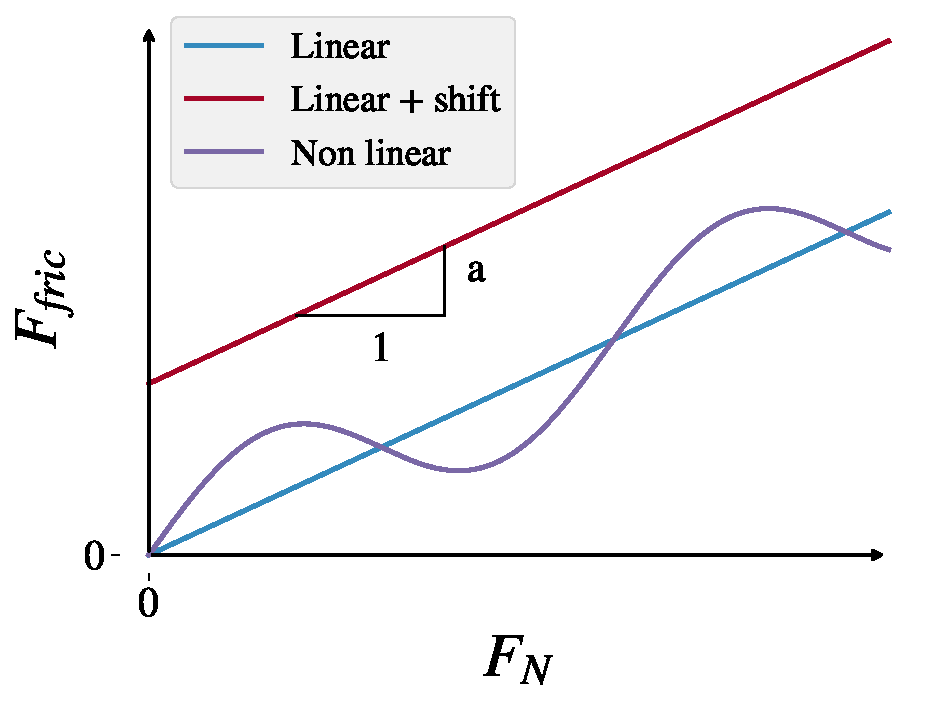
\includegraphics[width=\textwidth]{figures/theory/fric_coef_example_a.pdf}
      \caption{}
      \label{fig:fric_coef_example_a}
    \end{subfigure}
    \hfill
    \begin{subfigure}[t]{0.32\textwidth}
      \centering
      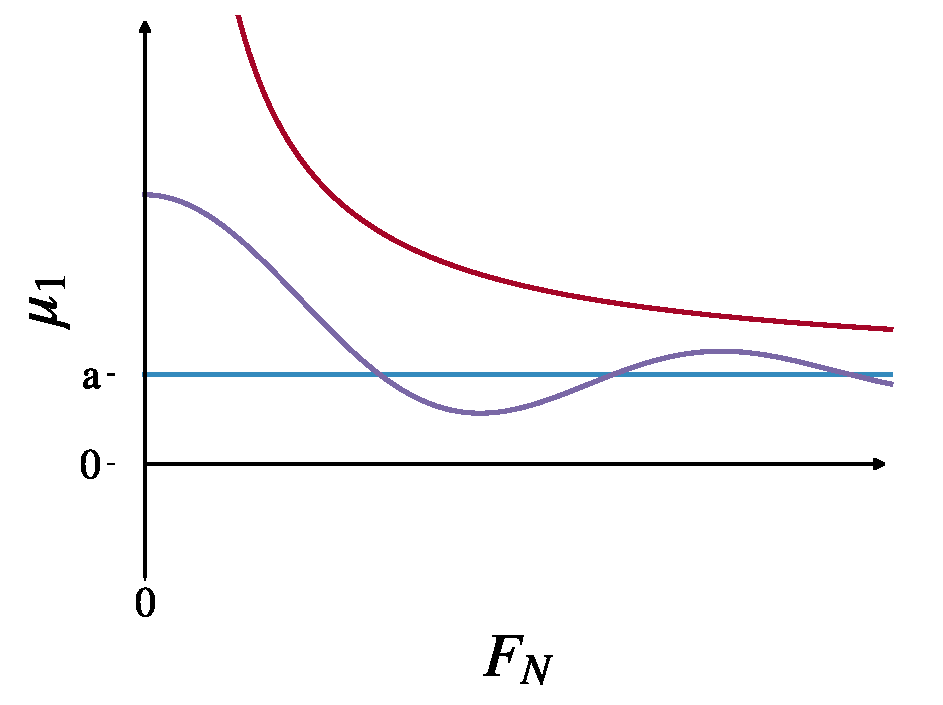
\includegraphics[width=\textwidth]{figures/theory/fric_coef_example_b.pdf}
      \caption{}
      \label{fig:fric_coef_example_b}
    \end{subfigure}
    \hfill
    \begin{subfigure}[t]{0.32\textwidth}
      \centering
      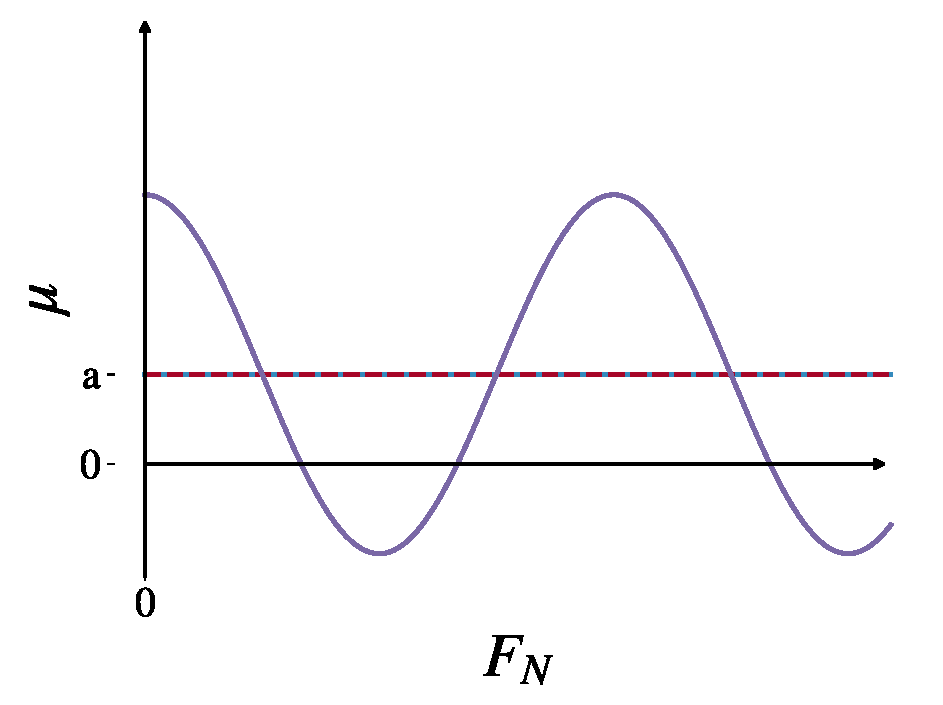
\includegraphics[width=\textwidth]{figures/theory/fric_coef_example_c.pdf}
      \caption{}
      \label{fig:fric_coef_example_c}
  \end{subfigure}
  \hfill
  \caption{Illustration of the consequences for the two definitions of the friction coefficient in~\cref{eq:mu_def}. (a) Three examples of friction-load curves consisting of a typical linear curve (blue), a linear curve with a shift representing an adhesive contact (red), and a non-linear curve (purple). The corresponding friction coefficients $\mu_1$ and $\mu_2$ are shown for the first definition~\cref{eq:mu_def1} in (b) and the second definition~\cref{eq:mu_def1} in (c).}
  \label{fig:fric_coef_example}
\end{figure}

% (b) The friction coefficient $\mu_1$ by definition of~\cref{eq:mu_def1}. (c) The friction coefficient $\mu_2$ by definition of~\cref{eq:mu_def2}

Amontons’ law represents the behavior relatively accurately for many surfaces in contact, involving both dry and lubricated, ductile and brittle and rough and smooth surfaces (as long as they are not adhesive) under a variety of conditions~\cite{gao_frictional_2004}. But it has its limitations. For instance, at low velocities, Amontons' model breaks down due to thermal effects, and for high velocities due to inertial effects~\cite[pp.\ 5--6]{gnecco_meyer_2015}. Additionally, static friction depends on the so-called contact history, with increasing static friction as the logarithm of time in stationary contact~\cite{dieterich_1972}.

In cases where Amontons' law breaks down, we might still use the conceptual
definition of the friction coefficient as defined by~\cref{eq:mu_def2}.
Especially, in the context of achieving negative friction coefficients (for certain load ranges), we would refer to this definition, since~\cref{eq:mu_def1}
would imply a truly unphysical situation of the frictional force acting in the
same direction as the sliding motion. This would accelerate the object
indefinitely\footnote{You would most likely have a good shot at the Nobel Prize
with that paper.}.

Due to the empirical foundation of Amontons’ law, it does not provide any
physical insight into the underlying mechanisms of friction. However, as we will
later discuss in more detail, we can understand the overall phenomena of
friction through statistical mechanics by the concept of \textit{equipartition
of energy}~\cite{Manini_2016}. A system in equilibrium has its kinetic energy
uniformly distributed among all its degrees of freedom. When a macroscale object
is sliding in a given direction it is clearly not in equilibrium since one of
its degrees of freedom carries considerably more kinetic energy. Thus, the
system will tend to transfer kinetic energy to the remaining
degrees of freedom in the form of heat dissipating to the surroundings. This will make the object slow down if not continuously driven forward by an external energy source. Hence, we can understand the overall concept of friction simply
as the tendency of going toward equilibrium energy equipartitioning among many
interacting degrees of freedom~\cite{Manini_2016}. From this point of view, it is
clear that friction is an inevitable part of contact physics, but even though
friction cannot be removed altogether, we are still capable of manipulating it
in useful ways. \\
\\
The attentive reader might point out that we have already moved the discussion
into the microscopic regime as \textit{statistical mechanics} generally
aim to explain macroscale behavior by microscopic interactions. This 
highlights the necessity to consider smaller scales in order to achieve a more fundamental understanding of friction.
\\
\\
We note that more advanced models for macroscale friction exist. For instance, the earthquake-like (EQ) model, also known as the \textit{spring-and-block} model or the \textit{multi-contact} model~\cite{Manini_2016}, developed by Burridge and Knopoff~\cite{Burridge_1967}. This has been used in many studies of earthquake friction~\cite{PhysRevLett.88.096102} and similar schemes have since been used to model the failure of fiber bundles and faults~\cite{newman_failure_1991, Smalley_1985}. Also, \textit{rate and state} models have been used for such macroscale modeling modeling~\cite{SELVADURAI2023229689}. However, these extensions are beyond the scope of this thesis as we will mainly focus on the nanoscale description. 



% All the terms in Amontons’ law refer to macroscopic, i.e., space- and time-averaged or “mean-field”, values. Thus, the contact area is the “apparent” or projected geometric area rather than the “real” contact area at the molecular level. And V is the mean relative velocity of the sliding bodies even though the shearing micro junctions may be moving with large fluctuations or in a stick-slip fashion.10~\cite{gao_frictional_2004}




% This includes taking the microscopic roughness
% into account together with surface chemistry. This more complex perspective
% introduces new (...() as real contact area, contact stresses, surface adhesion
% which makes frictional properties dependent on sliding speed, temperature and
% environment in general~\cite{kim_nano-scale_2009}. 


% The conclusion is that the friction coefficient is not an intrinsic physical
% property~\cite{Szlufarska_2008}.

% The basic difficulty of friction is intrinsic, involving the dissipative
% dynamics of large systems, often across ill-characterized interfaces, and
% generally violent and nonlinear~\cite{Manini_2016}


% The severity of the task is also related to the experimental difficulty to
% probe systems with many degrees of freedom under forced spatial confinement,
% that leaves very limited access to probing the buried sliding interface.
% Thanks to remarkable developments in nanotechnology, new inroads are being
% pursued and new discoveries are being made.~\cite{Manini_2016}


\section{Microscopic scale}\label{sec:microscale}
Going from a macro- to a microscale perspective, at a length scale on the order
\SI{e-6}{m}, it was realised that most surfaces are in fact rough~\cite{mo_friction_2009}. The contact between two surfaces consists of numerous
smaller contact points, so-called \textit{asperities}, which form junctions due to contact pressure and adhesion as visualized in~\cref{fig:asperity_contact}~\cite{kim_nano-scale_2009}. In the macroscale perspective of Amonton's law, we refer to time- and space-averaged values, i.e.\ the apparent contact area and the average
sliding speed~\cite{gao_frictional_2004}. However, microscopically we find the
real contact area to be much smaller than the apparent area~\cite{kim_nano-scale_2009}, and the shearing motion of local microjunctions to happen at large fluctuations rather than as one synchronized movement throughout the surface. 

It is generally accepted that friction is caused by two mechanisms: Mechanical
friction and chemical friction~\cite{kim_nano-scale_2009}. Mechanical
friction is the ``plowing'' of the surface by hard particles or said asperities
with an energy loss attributed to deformations of the asperity. While plastic
deformations, corresponding to wear, gives rise to an obvious attribution for
the energy loss, elastic deformations are also sufficient in explaining energy
loss due to phonon excitations. The assumption of plastic deformations
has been criticized as this is theorized only to be present at the beginning of
a surface contact while it is negligible for prolonged or repeated contacts~\cite{CARBONE20082555}. That is, when machine parts slide against each other for
millions of cycles, the plastic deformation would only take place at the beginning for which the system then reaches a steady state with only elastic deformations.
The chemical friction arises from adhesion between microscopic contacting
surfaces, with an energy loss attributed to the breaking and forming of chemical bonds between the interacting surfaces. 



\subsection{Asperity theories} % Surface roughness --- Asperity theories
% Sources in general:~\cite{mo_friction_2009},~\cite{kim_nano-scale_2009} \\

Asperity theories have their foundations in the adhesion model proposed by Bowden and Tabor~\cite{bowden2001friction} which is based on the fundamental reasoning that friction is governed by the adhesion between two surfaces~\cite{Kim_2012}. Adhesion is proportional to the real contact area defined by asperity junctions, and interfacial shear strength $\vec{\tau}$ between such contacting junctions. For an asperity contact area $A_{\text{asp}}$ we get a true contact area $\sum A_{\text{asp}}$ leading to 
\begin{align*}
  F_\text{fric} = \vec{\tau} \sum A_{\text{asp}}.
\end{align*}
Note that this is still compatible with Amontons’ law in~\cref{eq:amonton} by having a linear relationship between the real contact area and the
applied load. In fact, this is exactly how the theoretical model explains the friction dependency of load. By increasing the normal load it is hypothesized that the real contact area will increase as the asperity tips are deformed (plastically or elastically) into broader contact points as visualized qualitatively in~\cref{fig:asperity_contact}.

\begin{figure}[H]
  \centering
  \begin{subfigure}[b]{0.49\textwidth}
      \centering
      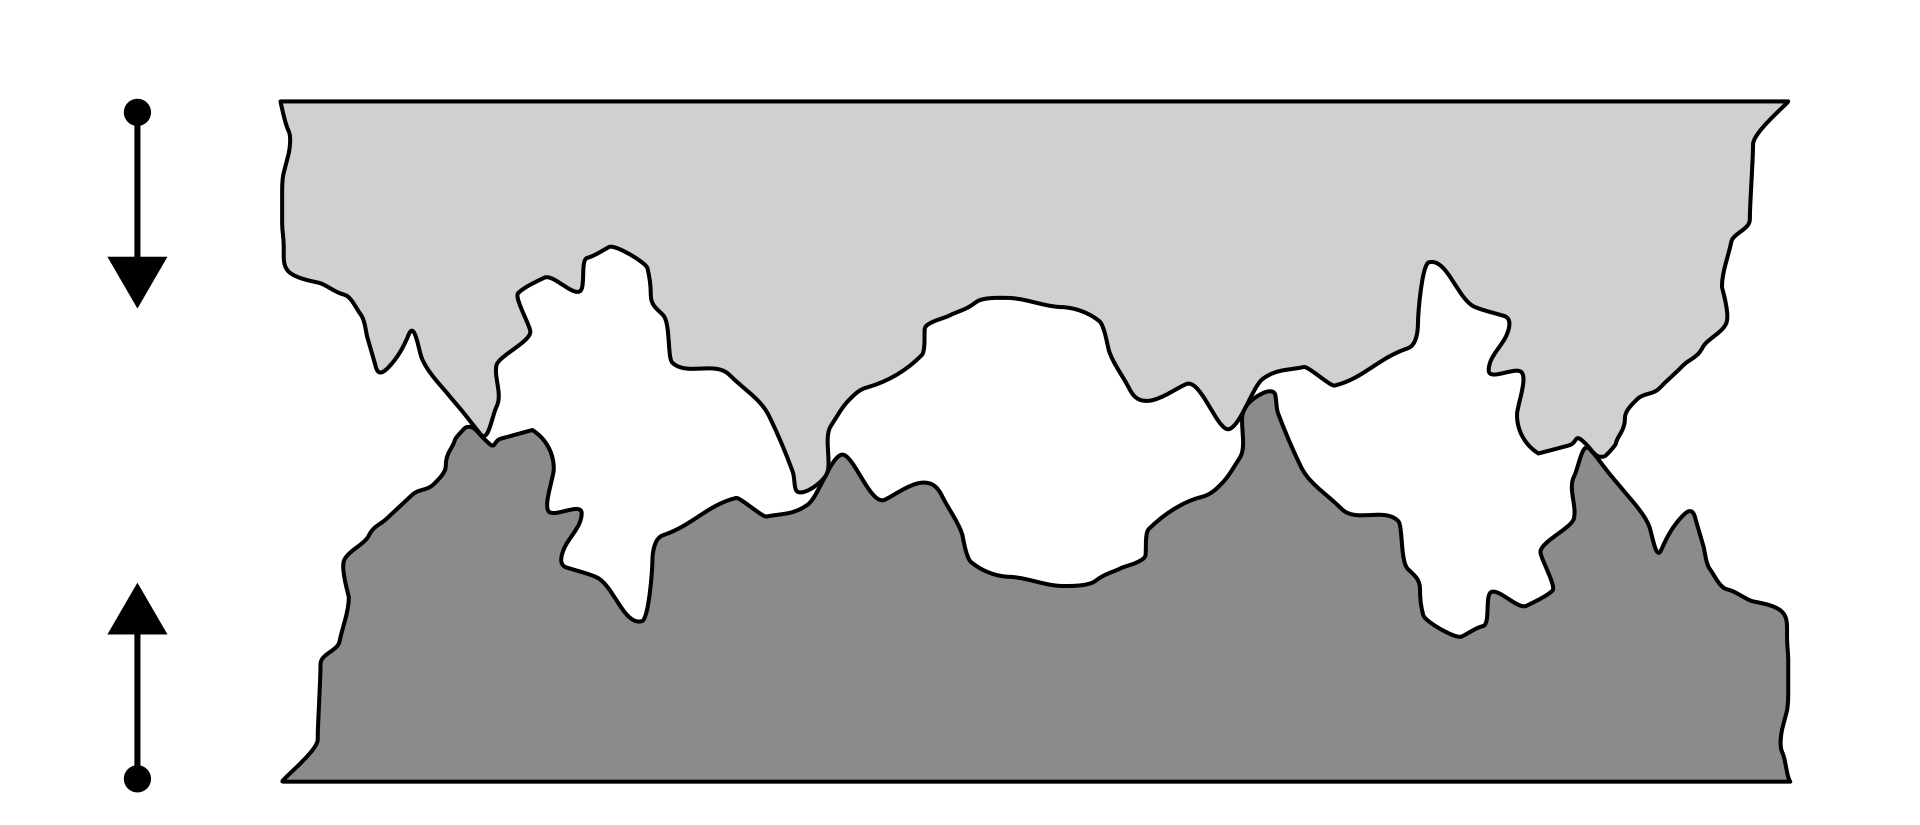
\includegraphics[width=\textwidth]{figures/theory/asperities_top.png}
      \caption{Low load.}
      \label{fig:asp_left}
  \end{subfigure}
  \hfill
  \begin{subfigure}[b]{0.49\textwidth}
      \centering
      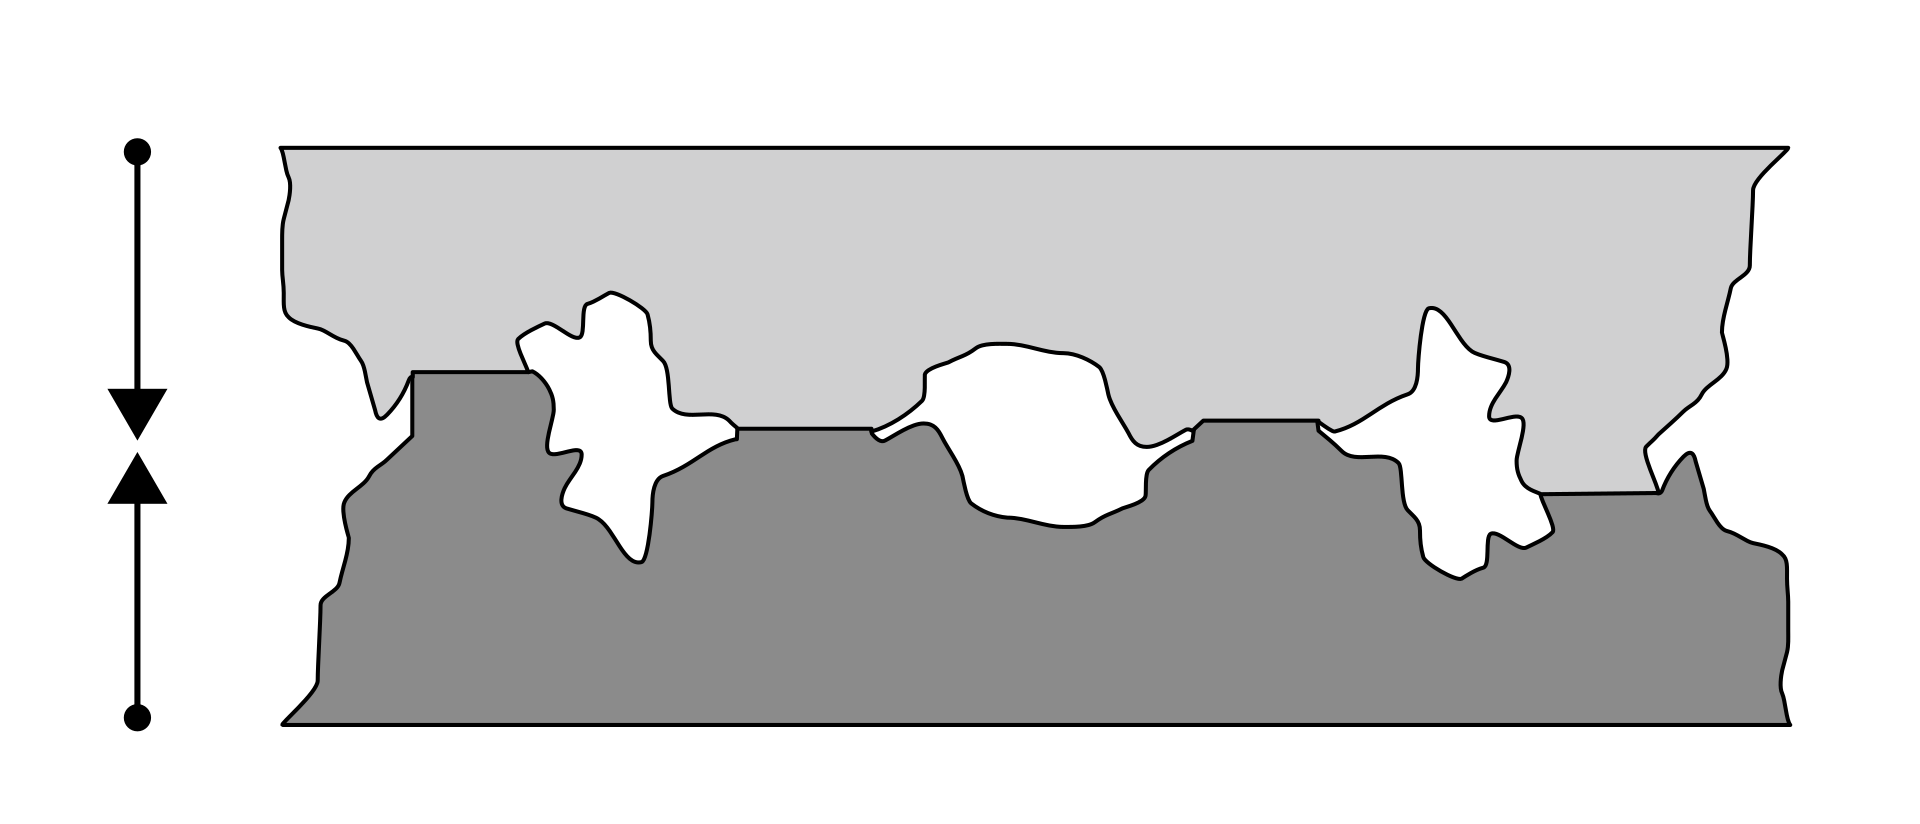
\includegraphics[width=\textwidth]{figures/theory/asperities_bottom.png}
      \caption{High load.}
      \label{fig:asp_right}
  \end{subfigure}
  \hfill
     \caption{Qualitatively illustration of the microscopic asperity deformation
     under increasing load from frame (a) to (b). While this figure seemingly portrays plastic deformation the concept of increased contact area with increased load applies to elastic deformation as well. Reprinted from ~\cite{wiki:asperities}.}
     \label{fig:asperity_contact}
\end{figure}

Many studies have focused on single asperity contacts to reveal the relationship
between the contact area and load~\cite{Szlufarska_2008, PhysRevLett.56.930,
perry_scanning_2004}. By assuming perfectly smooth asperities, with radii of
curvature from micrometers all the way down to nanometers, continuum mechanics
can be used to predict the deformation of asperities as load is applied. A model
for non-adhesive contact between homogenous, isotropic, linear elastic spheres
was first developed by Hertz~\cite{HertzOnTC}, which predicted $A_{\text{asp}}
\propto F_N^{2/3}$. Later adhesion effects were included in a number of
subsequent models, including Maugis-Dugdale theory~\cite{MAUGIS1992243}, which
also predicts a sublinear relationship between $A_{\text{asp}}$ and $F_N$. Thus,
the common feature of all single-asperity theories is that $A_{\text{asp}}$ is a
sublinear function of $F_N$, leading to a similar sublinear relationship for
$F_\text{fric}(F_N)$. This fails to align with the macroscale observations
modeled by Amontons’ law (\cref{eq:amonton}).

% Concurrently with single-asperity studies, roughness contact theories are being developed8–10,16 to bridge the gap between the mechanics of single asperities and that of macroscopic contacts.\cite{mo_friction_2009}

Concurrently with single-asperity studies, roughness contact theories are being developed~\cite{PhysRevLett.100.055504, Persson, GW, BUSH197587} to bridge the gap between single asperities and macroscopic contacts~\cite{mo_friction_2009}. A variety of multi-asperity theories has attempted to combine single asperity
mechanics by statistical modeling of the asperity height and spatial
distributions~\cite{CARBONE20082555}. This has led to partial success in the establishment of a linear relationship between $A_{\text{asp}}$ and $F_N$. Unfortunately, these results are restricted in terms of the magnitude of the load and contact area, where multi-asperity
contact models based on the original ideas of Greenwood and Williamson~\cite{GW}
only predicts linearity at vanishing low loads, or Persson~\cite{Persson} which predicts linearity for more reasonable loads up to 10--15\% of the macroscale contact area. However, as the load is further increased all multi-asperity models
predict the contact area to fall into the sublinear dependency of normal force
as seen for single asperity theories as well~\cite{CARBONE20082555}.


% Da Vinci-Amontons law – friction independent of the area – is not confirmed at
% the microscopic scale. In most nanoscale investigations the friction of a
% single con- tact is found to increase linearly with the contact area [27–29].
% In contrast, structurally mismatched atomically flat and hard crystalline or
% amorphous surfaces are expected to produce a sublinear increase in friction
% with contact area. The frequent finding of friction proportional to the area
% even in some of these cases can be understood as a consequence of softness,
% either if the interface, or surface contaminants lead to effectively pseudo-
% commensurate interfaces [30, 31] (Current trends in the physics of nanoscale
% friction)


% Other authors proposed an empirical model in which mechanics of a nanoscale non-adhesive contact is controlled by load, that is, $F_f = \mu L$ and the contact area is undefined and unnecessary5,29~\cite{mo_friction_2009}

%~\cite{mo_friction_2009} agues that the break-down of single-asperity theories
% of friction is due to the asperity (circumference defined) area is not
% proportional to the real one. By obtaining the real area (contacting bond) he
% arrives at the macroscale relationship... Quote: As shown in Table 1, the
% friction force is now proportional to contact area at all length scales as
% long as the contact area is correctly defined at each length scale. When
% adhesion is added they arrive at the sublinear trend again. 



% Our model predicts that as the adhesion between the contacting surfaces is reduced, a transition takes place from nonlinear to linear dependence of friction force on the load.~\cite{mo_friction_2009}




% This approach enables the bottom-up derivation of the linear scaling laws of macroscopic friction with size, and their transition to the sublinear ones for incommensurate nanosized contacts. We can now understand that such transition takes place when the contact roughness becomes large compared to the range of interfacial interactions [162]~\cite{Manini_2016}.


% However, practical single- and multiple-contact conditions are characterized by
% complex interaction profiles plus nontrivial internal dynamics. As a result,
% the interplay of thermal drifts, contact aging, contact-contact interactions,
% and macroscopic elastic deformations introduce significant complications, and
% make the depinning transition from static to kinetic friction an active field
% of research.~\cite{Manini_2017}[p. 2]. 


% However, even though the successes of continuum mechanics there is no reason to
% believe that it will be capable of reproducing tribological behavior at the
% nanometre length scale where the discreteness of atoms often has a direct effect
% on physical properties~\cite{Szlufarska_2008}.


%
\section{Nanoscale --- Atomic scale}\label{sec:nanoscale}
% In the need for a review of the relevant stuff read: https://arxiv.org/pdf/1112.3234.pdf
Going from a micro- to a nanoscale, on the order of \SI{e-9}{m}, it has been
predicted that continuum mechanics will start to break down~\cite{luan_breakdown_2005} due to the discreteness of individual atoms. In a
numerical \acrshort{MD} study by Mo et al.~\cite{mo_friction_2009}, considering
asperity radii of 5--30 nm, it has been shown that the asperity area
$A_{\text{asp}}$, defined by the circumference of the contact zone, is
sublinear with $F_N$. This is accommodated by the observation that not all atoms
within the circumference make chemical contact with the substrate. By modeling
the real contact area $A_{\text{real}} = NA_{\text{atom}}$, where $N$ is the
number of atoms within the range of chemical interaction and $A_{\text{atom}}$
the associated surface area for a contacting atom, they found a consistent linear relationship between friction and the real contact area. Without adhesive
forces, this leads to a similar linear relationship $F_{\text{fric}} \propto F_N$,
while adding van der Waals adhesion to the simulation gave a sublinear
relationship matching microscale single asperity theory, even though the
$F_{\text{fric}} \propto A_{\text{real}}$ was maintained. This result emphasizes
that the predictions of continuum mechanisms might still apply at the nanoscale
and that the contact area can be expected to play an important role in
nanoscale asperity contacts. It is simply the definition of the contact area that
changes when transitioning from micro- to nanoscale. 


% Although both numerical~\cite{zhu_study_2018}\cite{ma12091425}\cite{bonelli_atomistic_2009} and experimental~\cite[2005]{DIENWIEBEL2005197}\cite{feng_superlubric_2013} studies have been done for so-called nanoflakes
% sliding on a substrate, the dependence of friction force on contact area is not investigated.  One reasonable explanation is that the contact area is already at its maximum for atomically smooth contacting surfaces and hence does not play an important role. In a numerical study of atomic-scale frictional behavior of corrugated nano-structured surfaces~\cite{C2NR30691C} they reported that the contact area only affected the friction significantly for big corrugations as opposed to small. Since increasing friction is still reported under increasing load in most nanoflake studies (see
% \cref{sec:expected_prop} for a more detailed discussion), this suggests
% that some other mechanisms are governing friction at this level. 


% make it unfounded to rely on asperity theories.

% Note that atom spacing lies in the
% domain of a few ångströms Å (\SI{e-10}{m}) and thus we take the so-called
% atomic-scale to be a part of the nanoscale regime. 

% ``Load-independent friction has also been observed in FFM experiments on thermally oxidized MoS2, and it was proposed that MoO3 nanocrystals, that grew during the oxidation process on the MoS2 surface [35], acted as a spacer between the tip and the sample, such that the contact area remained unchanged upon loading. In the present case, the contact area would be completely determined by the flake size, which would be independent of the loading force. Hence, the friction would only increase slightly with the normal load as the result of the increase in contact pressure.''~\cite{DIENWIEBEL2005197}

% Before diving into alternative theoretical approaches to address this issue we point out that exactly this transition, between nanoscale asperities and atomically smooth surfaces, is of outermost importance for the objective of the thesis. By introducing kirigami cuts and stretching the sheet we expect to see an out-of-plane buckling which induces an ensemble of asperities on the sheet. Hence, we might hypothesize that such a transition will contribute to a significant change in the governing mechanism of friction bridging the two domains of nanoscale asperity and smooth surface theory. 

While the study by Mo et al.~\cite{mo_friction_2009} considers a single
asperity on a nanoscale, some models take this even further to what we will
denote as the atomic scale. This final leap is motivated by the fact that our
system of interest, an atomically flat graphene sheet imposed on a flat silicon
substrate, lacks the presence of nanoscale asperities in its initial uncut
undeformed state. In the lack of noteworthy structural asperities, friction can
instead be modeled as a consequence of the ``rough'' potential laid out by
the atomic landscape. A series of so-called \textit{reduced-order} models build on a
simplified system of atomic-scale contacts based on three essential parts: 1) A
periodic potential modeling the substrate as a rigid crystalline surface. 2) An
interacting particle, or collection of particles, placed in the potential. 3) A
moving body, moving at a steady speed, connected to the particles through a
harmonic spring. In figure~\cref{fig:PT_FK_FKT} three of the most common 1D
models are displayed which we will address in the following sections. The
time-honored Prandtl-Tomlinson (\acrshort{PT}) model describes a point-like tip sliding
over a space-periodic fixed crystalline surface with a harmonic coupling to the
moving body. This is analog to that of an experimental cantilever used for
Atomic Force Microscopy which we will introduce in more detail in~\cref{sec:SPM}. Further extensions were added in the Frenkel-Kontorova
(\acrshort{FK}) model by substituting the tip with a chain of harmonically coupled
particles dragged from the end, and finally combined in the
Frenkel-Kontorova-Tomlinson (\acrshort{FKT}) with the addition of a more
rigorous harmonic coupling between the moving body and each of the atoms in the
chain. While these models cannot provide the same level of detail as atomistic
simulations, such as \acrshort{MD}, they enable investigation of atomic friction
under most conditions, some of which are inaccessible to \acrshort{MD}~\cite{Yalin_2011}. This makes these models an appropriate tool for investigating
individual parameters and mechanisms governing friction.


\begin{figure}[H]
  \centering
  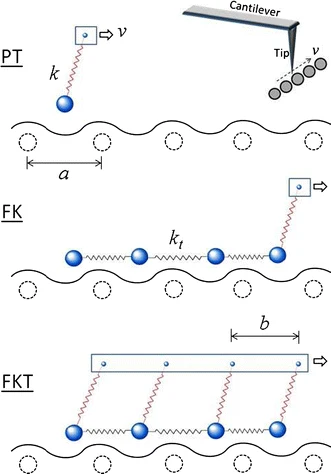
\includegraphics[width=0.4\linewidth]{figures/theory/PT_FK_FKT.png}
  \caption{Illustration of the key features of the Prandtl-Tomlinson (\acrshort{PT}), Frenkel-Kontorova (\acrshort{FK}) and Frenkel-Kontorova-Tomlinson (\acrshort{FKT}) respectively~\cite{Yalin_2011}. Reproduced from~\cite{Yalin_2011}.}
  \label{fig:PT_FK_FKT}
\end{figure}


% Analytical Models for Atomic Friction~\cite{Yalin_2011}
% \textbf{Analytical Models for Atomic Friction}
\subsection{Prandtl–Tomlinson} % Sources for PT model~\cite[2,3]{Yalin_2011} 
The Prandtl–Tomlinson model (\acrshort{PT}) considers a 1D simplification of
the frictional system as a single ball-tip sliding along the rigid substrate as
shown in~\cref{fig:PT_FK_FKT}. The tip is coupled harmonically to a moving support, moving at a constant speed, which drives the tip forward. The interaction between
the tip and the substrate is modeled by a sinusoidal corrugation potential
mimicking the periodicity found in a crystalline substrate. We will consider the
Prandtl–Tomlinson model with added thermal activation as proposed by Gnecco et
al.~\cite{PhysRevLett.84.1172}. For the theoretical foundation of this section,
we generally refer to~\cite{Yalin_2011}. The potential energy for the tip at position $x$ for time $t$ is given as
\begin{align}
  V(x,t) = \frac{1}{2}K(vt - x)^2 - \frac{1}{2}U_0 \cos \left(\frac{2\pi x}{a} \right).
  \label{eq:V_PT}
\end{align}
The first term describes the harmonic coupling with spring constant $K$, between the tip at position $x$ and the moving body at position $vt$, given by its constant speed $v$. The second term describes the corrugation potential with amplitude $U_0$ and period $a$ representing the lattice spacing of the substrate. The dynamics of the tip can be described by the Langevin equations 
\begin{align}
  m \ddot{x}+m \mu \dot{x}=-\frac{\partial V(x, t)}{\partial x}+R(t),
  \label{eq:Langevin_PT}
\end{align}
where $m$ is the mass of the tip, $\mu$ the viscous friction and $R(t)$ the thermal activation term. The equation is solved for tip position $x$ and the friction force is retrieved as the force acting on the moving body
\begin{align*}
  F_{\text{fric}} = K(vt - x).
\end{align*}
The governing equation~\cref{eq:Langevin_PT} belongs to a family of stochastic differential equations composed of both deterministic dynamics and stochastic processes. In this case, the deterministic term is the viscous friction, $m\mu\dot{x}$, to resist the movement of the tip and the force acting from the corrugation potential. The stochastic term is a random force field modeling thermal noise according to the Fluctuation-dissipation relation. Thus, there is no single path but rather multiple paths the tip can take. While the Langevin equation is one of the most common ways to handle thermal activation other methods exist to solve this problem such as Monte Carlo sampling methods. We omit the numerical scheme for the solving of the Langevin equations here and refer instead to a more in-depth discussion of the Langevin equation regarding the \acrshort{MD} simulations in~\cref{sec:langevin}. 


\subsubsection{Thermal activation}
The solving of the Langevin equation, as opposed to Newton's equation of motion, introduces thermal effects to the system. Generally, when the energy barrier comes close to $k_B T$ (\SI{0.026}{eV} at room temperature) thermal effects can not be neglected. In the case of a single asperity contact the energy barrier is on the order \SI{1}{eV} which makes thermal activation significant~\cite{Yalin_2011}. Due to the moving body traveling at a constant speed, the potential energy will increase steadily. Without any temperature, $T = 0$, the slip will only occur when the energy barrier between the current potential well $(i)$ and the adjacent $(j)$ is zero $\Delta V_{i\to j} = 0$. However, in the presence of temperature, we get thermal activation, meaning that the tip can slip to the next potential well sooner at $\Delta V_{i\to j} > 0$. Provided that the sliding speed is slow enough the transition rate $\kappa$ for a slip from the current to the next well is given by
\begin{align}
  \kappa = f_0 e^{-\Delta V / k_B T},
  \label{eq:PT_kappa}
\end{align}
with $\Delta V$ being the energy barrier and $f_0$ the attempt rate. The attempt rate following Kramer’s rate theory~\cite{RevModPhys.62.251} is related to the mass and damping of the system and can be thought of as the frequency at which the tip ``attempts'' to overcome the barrier. Notice that~\cref{eq:PT_kappa} resembles a microstate probability in the canonical ensemble with $f_0$ in place of the inverse partition function $Z^{-1}$ which provides an additional interpretation of $f_0$. The probability $p_i$ that the tip occupies the current well $(i)$ relative to the adjacent well $(j)$, as illustrated in~\cref{fig:PT_slip} is governed by 
\begin{align}
  \frac{dp_i}{dt} = -\kappa_{i\to j}p_i + \kappa_{j\to i}p_j.
  \label{eq:dpdt_PT}
\end{align}
This probability is related to temperature, speed and mass~\cite{Yalin_2011}.

\begin{figure}[H]
  \centering
  \includegraphics[width=0.5\linewidth]{figures/theory/PT_slip.png}
  \caption{An illustration of slip between two adjacent energy minima. $p_i$ is the probability of the tip residing in the current potential well, $i$, where the energy barrier is $\Delta V_{i \rightarrow j}$. $p_j$ is the probability of the tip residing at the next minima, $j$, where $\Delta V_{j \rightarrow i}$ is the corresponding energy barrier. Figure and caption reproduced from~\cite{Yalin_2011}.}
  \label{fig:PT_slip}
\end{figure}


Generally, there exist two temperature regimes in the Prandtl–Tomlinson model: The \textit{thermal activation} regime at low temperatures and the \textit{thermal drift} at high temperatures as shown in~\cref{fig:PT_temp}. At lower temperatures, the system is subject to standard thermal activation with a much lower energy barrier for slipping forward than backward $\Delta V_{j \to i} \gg \Delta V_{i \to j}$. This results in a higher transition rate for forward slips, $\kappa_{j \to i} \ll \kappa_{i \to j}$, which effectively inhibits any backward slip. This leads to the simplified expression for~\cref{eq:dpdt_PT}
\begin{align*}
  \frac{dp_i}{dt} = -\kappa_{i\to j}p_i,
\end{align*}
which makes the relationship between friction, temperature and speed follow Sang et al.’s prediction~\cite{Sang_2001}
\begin{align}
  F=F_c-\left|\beta k_B T \ln \left(\frac{v_c}{v}\right)\right|^{2 / 3}, \qquad v_c = \frac{2f_0\beta k_B T}{3 C_{\text{eff}} \sqrt{F_c}},
  \label{eq:F_thermal_ac}
\end{align}
where $F_c$ is the maximum friction at $T = 0$, $v_c$ a critical velocity, $f_0$
is the attempt rate, $c_{eff}$ the effective stiffness, and $\beta$ a
parameter determined by the shape of the corrugation well. \cref{eq:F_thermal_ac} characterizes the decrease in friction with temperature
in the thermal activation regime, shown in~\cref{fig:PT_temp_a} at low temperature. This corresponds with the assumption of only forward slips, as seen in the force trace in~\cref{fig:PT_temp_a}. When the temperature is high enough for the system to be consistently close to thermal equilibrium, it enters the regime of thermal drift~\cite{PhysRevE.71.065101}. This regime transition can be understood through a comparison between two time scales: The time it takes for the moving body to travel one lattice spacing
$t_v = a/v$ and the average time for a slip to occur due to thermal activation
$\tau = 1/\kappa = f^{-1}\exp(\Delta V / k_BT)$. If $t_v \gg \tau$ the system falls within the thermal drift regime, where slips happen both in the forward and backward direction as shown in the force trace in~\cref{fig:PT_temp_b}. For the thermal drift regime, the friction follows the prediction by Krylov et
al.~\cite{Krylow_2007, PhysRevE.71.065101, Jinesh_2008}
\begin{align}
  F \propto \frac{v}{T}e^{1/T}.
  \label{eq:PT_thermal_drift}
\end{align}
Notice that the friction dependence on sliding speed changes from~\cref{eq:F_thermal_ac} to~\cref{eq:PT_thermal_drift} as it transitions from the thermal activation to the thermal drift regime. 


\subsubsection{Sliding speed}
In the thermal activation regime (low temperature) and at low sliding speeds, the
friction relation follows~\cref{eq:F_thermal_ac} which means that friction
increases logarithmically with speed. For higher speeds, above the critical
velocity $v > v_c$, if only thermal effects are considered,
\cref{eq:F_thermal_ac} predicts that friction will eventually saturate and come
to a plateau at $F_{\text{fric}} = F_C$. This is illustrated in
\cref{fig:PT_speed} with this prediction being represented by the dotted line.
However, as given away by the figure, for higher speeds the model will enter an
\textit{athermal} regime where the thermal effects are negligible compared to
other contributions~\cite{PhysRevLett.89.224301}. In the athermal regime, the
damping term $m\mu \dot{x}$ will dominate yielding $F_{\text{fric}}\propto v$.
The athermal regime is often observed in reduced-models if the system is
overdamped or at high speeds. This concept is related to \acrshort{MD}
simulations as well where the accessible speeds often fall into the athermal
regime~\cite{Li_2011}. It is unclear how this affects real physical systems for
which there exist more dissipation channels than just a single viscous
term~\cite{Dong_2013}. For the thermal drift regime, at higher temperatures, friction increase linearly with sliding speed $F_{\text{fric}} \propto v$ as given by~\cref{eq:PT_thermal_drift}.


\begin{figure}[!htb]
  \centering
  \begin{subfigure}[t]{0.49\textwidth}
      \centering
      \includegraphics[width=\textwidth]{figures/theory/PT_temp.png}
      \caption{}
      \label{fig:PT_temp_a}
  \end{subfigure}
  \hfill
  \begin{subfigure}[t]{0.49\textwidth}
      \centering
      \includegraphics[width=\textwidth]{figures/theory/PT_temp_force.png}
      \caption{}
      \label{fig:PT_temp_b}
  \end{subfigure}
  \hfill
  \hfill
     \caption{Illustration of the temperature difference between the thermal activation regime and the thermal drift regime. (a) shows the mean friction as a function of temperature showcasing the regime transition. The figure corresponds to the numerical results of Dong et al.~\cite{Yalin_2011} of a Prandtl–Tomlinson model with model parameters: $m=\SI{e-12}{kg}$, $U_0={0.6}{eV}$, $v=\SI{4e3}{nm/s}$, $\mu=\SI{2}{\sqrt{k/m}}$, $a=\SI{0.288}{nm}$. (b) shows the force traces of a simulation in the thermal activation regime (top) and thermal drift regime (bottom) with several characteristic forward and backward slips identified by dashed lines for the latter case. Reproduced from~\cite{Yalin_2011}.}
     \label{fig:PT_temp}
\end{figure}



\begin{figure}[!htb]
  \centering
  \includegraphics[width=0.5\linewidth]{figures/theory/PT_speed.png}
  \caption{The friction dependence on sliding speed for the simulated Prandtl–Tomlinson by Dong et al.~\cite{Yalin_2011} revealing two different regimes. In the thermal regime, friction increases logarithmically with speed, and in the athermal regime, friction is governed by damping such that $F\propto v$. The friction plateau ($F_c = \SI{0.39}{nN}$) predicted by thermal activation is shown as a dotted line. Other models parameters: $m=\SI{e-12}{kg}$, $U_0={0.6}{eV}$, $T = \SI{300}{K}$, $\mu=\SI{2}{\sqrt{k/m}}$, $a=\SI{0.288}{nm}$. Reproduced from~\cite{Yalin_2011}.}
  \label{fig:PT_speed}
\end{figure}


\subsubsection{Tip mass}
The mass of the tip affects the dynamics due to a change of inertia, which changes the attempt rate $f_0$. Smaller inertia leads to a larger attempt rate and vice versa. Effectively, this will affect the transition point for the temperature and speed regimes described previously. A smaller inertia, giving a larger attempt rate, will cause an earlier transition (i.e.\ at a lower temperature) to the thermal drift regime. Additionally, this will result in a later speed saturation such that it transitions to the athermal regime at a higher speed. 


\subsubsection{Friction Regimes: Smooth Sliding, Single Slip, and Multiple Slip}
Stick-slip motion is a crucial instability mechanism associated with high energy dissipation and high friction. Thus, controlling the transition between smooth sliding and stick-slip is considered key to controlling friction. We can divide the frictional stick-slip behavior into three regimes: 1) Smooth sliding, where the tip slides smoothly on the substrate. 2) Single slip, where the tip stick at one potential well before jumping one lattice spacing to the next. 3) Multiple slip, where the tip jumps more than one lattice spacing for a slip event. The underlying mechanisms behind these regimes can be understood through static and dynamic contributions. 

To understand the static mechanism we consider a quasistatic process for which temperature, speed and damping can be neglected. For a quasistatic process, we require $\partial(V)/\partial x = 0$. This simplifies~\cref{eq:V_PT} to 
\begin{align}
  \frac{\pi U_0}{a} \sin\left(\frac{2\pi x}{a}\right) \frac{2 \pi}{a} = K(vt - x).
  \label{eq:static_V}
\end{align}
The friction regime is determined by the number of solutions $x$ to~\cref{eq:static_V}. Only one solution corresponds to
smooth sliding, two solutions to a single slip and so on. It turns out that the
regimes can be defined by the parameter $\eta = 2\pi^2U_0/a^2K$~\cite{Johnson_1998, Medyanik_2006} yielding transitions at $\eta = 1, 4.6, 7.79, 10.95, \hdots$, such that $\eta \le 1$
corresponds too smooth sliding, $1<\eta \le 4.6$ to a single slip and so on. These static derivations lay out the fundamental probabilities for being in one of the stick-slip regimes. Notice that increasing the spring constant $K$ (stiff spring) will decrease the possibilities for stick-slip behavior. Similarly, the potential corrugation $U_0$ can be altered by an increasing load~\cite{Vanossi_2013}.

Considering the dynamics on top, one finds that damping, speed and temperature will affect this probability. High damping, equivalent to a high transfer
of kinetic energy to heat, will result in less energy available for the slip events. This will make multiple slip less likely. By a similar argument, we find that increasing the speed will contribute to more kinetic energy which will increase the likelihood of multiple slip. Finally, the temperature will contribute to earlier slips, due to thermal activation, such that
less potential energy can be accumulated and it will result in fewer multiple slip. 

% The effects of damping, speed and temperature are illustrated for the force traces in~\cref{fig:PT_slip_var}


% \begin{figure}[!htb]
%   \centering
%   \begin{subfigure}[t]{0.32\textwidth}
%       \centering
%       \includegraphics[width=\textwidth]{figures/theory/PT_slip_damping.png}
%       \caption{}
%   \end{subfigure}
%   \hfill
%   \begin{subfigure}[t]{0.32\textwidth}
%       \centering
%       \includegraphics[width=\textwidth]{figures/theory/PT_slip_speed.png}
%       \label{fig:PT_slip_vel}
%       \caption{}
%   \end{subfigure}
%   \hfill
%   \begin{subfigure}[t]{0.32\textwidth}
%       \centering
%       \includegraphics[width=\textwidth]{figures/theory/PT_slip_temp.png}
%       \caption{}
%   \end{subfigure}
%   \hfill
%      \caption{\hl{Temporary} figure from~\cite{Yalin_2011}. \hl{Consider removing since the interpretation of smooth sliding might get a bit tricky.}}
%      \label{fig:PT_slip_var}
% \end{figure}



% Together with the current experimental possibility to perform well-defined
% measurements on well-characterized materials at the fundamental microscopic
% level of investigation of the sliding contacts, advances in the computer
% modeling of interatomic interactions in materials science and complex systems
% encompass molecular-dynamics (MD) simulations of medium to large scale for the
% exploration of the tribo-dynamics with atomic resolution [4, 5].




\subsection{Frenkel-Kontorova}
% Based on~\cite{Manini_2016} and~\cite{FK2D}.
The Frenkel-Kontorova (\acrshort{FK}) model~\cite{Frenkel_1938} extends the Prandtl–Tomlinson model by considering a chain of atoms in contrast to just a single particle (tip). This extension is useful for understanding the importance of the alignment between the atoms and the substrate, the so-called \textit{commensurability}. Our review of the Frenkel-Kontorova is based on~\cite{Manini_2016, Vanossi_2013}.

The standard Frenkel-Kontorova model consists of a 1D chain of $N$ classical particles of equal mass, representing atoms, interacting via harmonic forces and moving in a sinusoidal potential as sketched in~\cref{fig:FK_model}~\cite{Manini_2016}. The Hamiltonian is 
\begin{align}
  H = \sum_{i=1}^N \left[\frac{p_i^2}{2m} + \frac{1}{2}K(x_{i+1} - x_i - a_c)^2 + \frac{1}{2}U_0 \cos{\left(\frac{2\pi x_i}{a_b}\right)}\right],
  \label{eq:H_FK}
\end{align}
where the atoms are labelled sequently $i = 1, \hdots, N$. The first term $p_i^2/2m$ represents the kinetic energy with momentum $p_i$
and mass $m$. Often the effects of inertia are neglected, referred to as the static Frenkel-Kontorova model, while the inclusion in‘\cref{eq:H_FK} is known as the dynamic Frenkel-Kontorova model~\cite{FK2D}. The next term describes the harmonic interaction with elastic
constant $K$, nearest neighbor distance $\Delta x = x_{i+1} - x_i$ and 
corresponding nearest neighbor equilibrium distance $a_c$. The final term represents the periodic corrugation potential, with amplitude $U_0$ and period $a_b$. By comparison to the potential used in the Prandtl–Tomlinson model~\cref{eq:V_PT}, the difference is the introduction of a harmonic coupling between particles in the chain as opposed to the moving body. Different boundary choices can be made where both free ends and periodic conditions give similar results. The choice of fixed ends however makes the chain incapable of sliding.

\begin{figure}[!htb]
  \centering
  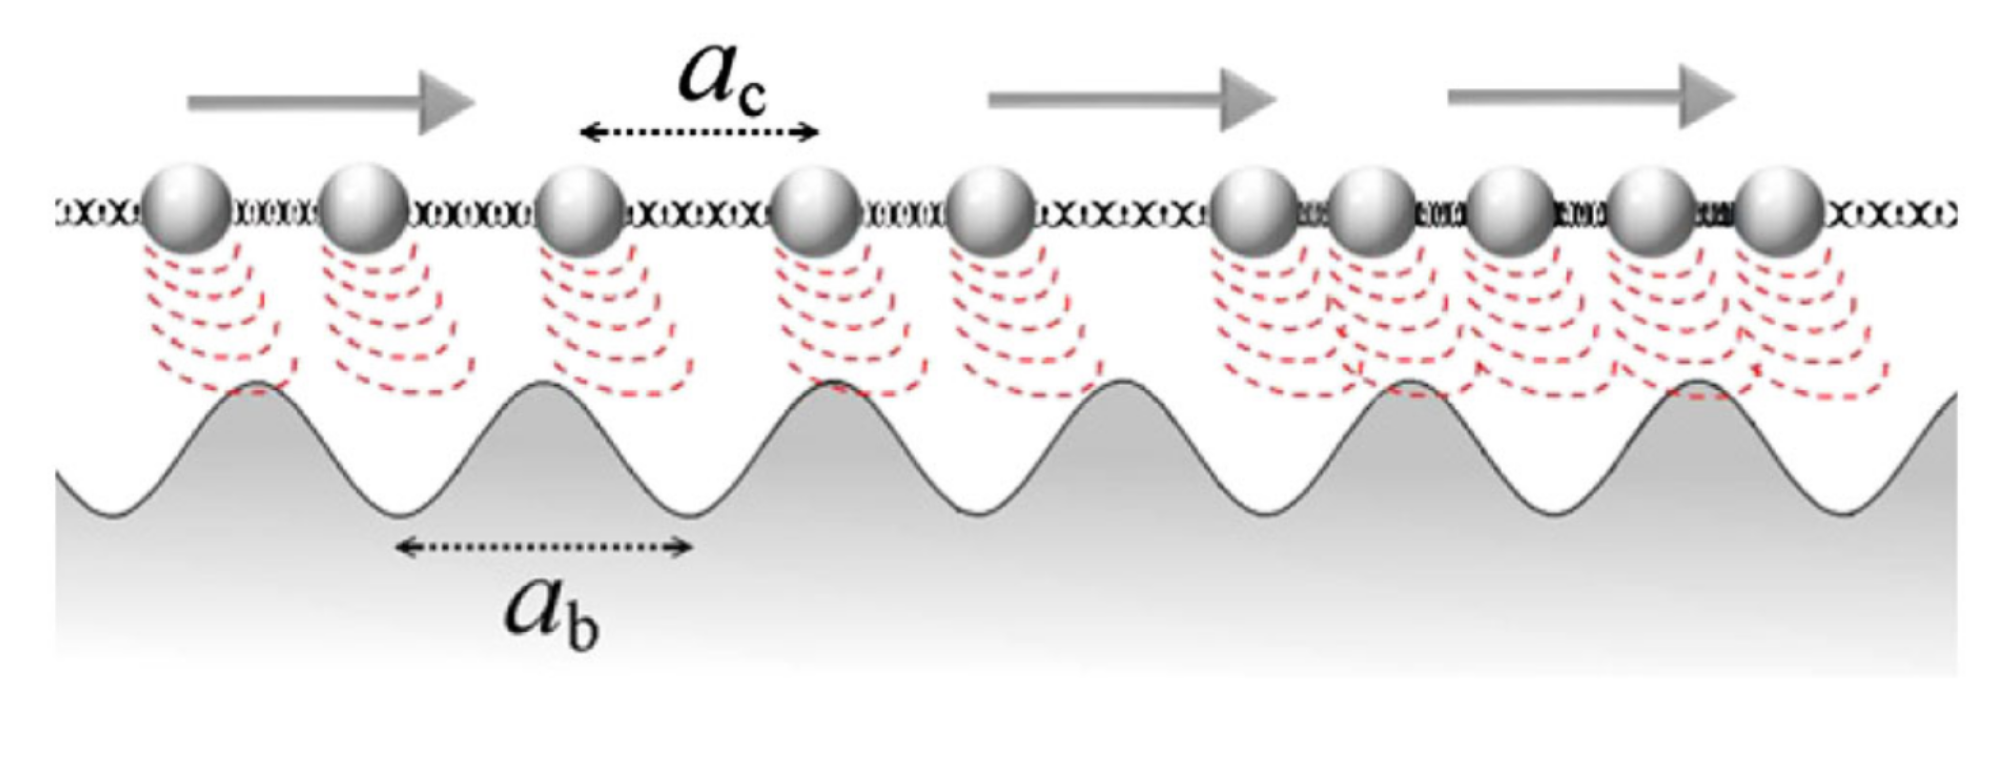
\includegraphics[width=0.6\linewidth]{figures/theory/FK_model.png}
  \caption{A sketch of the Frenkel-Kontorova model with the two competing lengths: interparticle and substrate periodicities. Figure and caption reproduced from~\cite{Vanossi_2013} with permission from the American Physical Society.}
  \label{fig:FK_model}
\end{figure}

To probe static friction one can apply an external adiabatically increasing force until sliding occurs, i.e.\ without loss or gain of heat. This corresponds to the static Frenkel-Kontorova model, and it turns out that the sliding properties are entirely governed by its topological excitations referred to as so-called \textit{kinks} and \textit{antikinks}

\subsubsection{Commensurability} We can subdivide the frictional behavior in terms of commensurability, that is, how well the spacing of the atoms matches the periodic substrate potential. We describe this by the length ratio $\theta = a_b / a_c = N / M$ where $M$ denotes the number of minima in the potential within the length of the chain. A rational number for $\theta$ means that we can achieve a perfect alignment between the atoms in the chain and the potential minima, without stretching the chain, corresponding to a \textit{commensurate} case. If $\theta$ is irrational the chain and substrate cannot fully align without some stretching of the chain, and we denote this as being \textit{incommensurate}.

We begin with the simplest commensurate case of $\theta = 1$ where the spacing
of the atoms matches perfectly with the substrate potential periodicity, i.e.\
$a_c = a_b$, $N = M$. The ground state (\acrshort{GS}) is the configuration
where each atom is aligned with one of the substrate minima. By adding an extra
atom to the chain we would effectively shift some of the atoms, out of this
ideal state, giving rise to a kink excitation. This leads to the case where two
atoms will have to ``share'' the same potential corrugation as sketched in
\cref{fig:incommensurable_example}. On the other hand, removing an atom from
the chain results in an antikink excitation where one potential corrugation will
be left ``atomless''. In order to reach a local minimum the kink (antikink) will
expand in space over a finite length such that the chain undertakes a local
compression (expansion). Notice that for low ratios of $\theta$, fewer atoms than minima, the chain will not be able to fill each corrugation well in any case. In this case, commensurability can instead be thought of as whether the atoms are forced to deviate, by a lattice spacing, from the spacing otherwise dictated by the spring forces in-between. When applying a tangential force to the chain it is much
easier for an excitation to move along the chain than it is for the non-excited
atoms since the activation energy for a kink/antikink
displacement is systematically smaller (often much smaller) than the potential
barrier $U_0$. Thus, the motion of kinks (antikinks), i.e.\ the displacement of
extra atoms (atom vacancies), is representing the fundamental mechanism for
mass transport. These displacements are responsible for the mobility,
diffusivity and conductivity within this model. 

\begin{figure}[!htb]
  \centering
  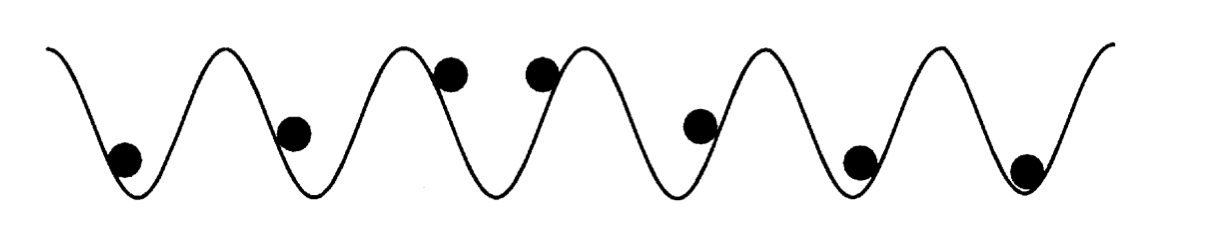
\includegraphics[width=0.55\linewidth]{figures/theory/incommensurable_example.png}
  \caption{Qualitative example of an incommensurable case where the atoms sit slightly closer together than otherwise dictated by the substrate potential. This results in a single kink here seen as the presence of two atoms within the same potential corrugation well. Reproduced from~\cite{BRAUN19981}.}
  \label{fig:incommensurable_example}
\end{figure}


In the zero temperature commensurable case with an adiabatical increase in force, all atoms would be put into an accelerating motion as soon as the potential barrier energy is present. However, similar to our discussion on the Prandtl-Tomlinson model, thermal activations will excite the system at an earlier stage resulting in kink-antikink pairs traveling down the chain. For a chain of finite length, these often occur at the end of the chain running in opposite directions. This cascade of kink-antikink excitations is shown in~\cref{fig:kink_antikink}. Notice, that for the 2D case, where an island (flake) is deposited on a surface, we generally also expect the sliding to be initiated by kink-antikink pairs at the boundaries. 


\begin{figure}[!htb]
  \centering
  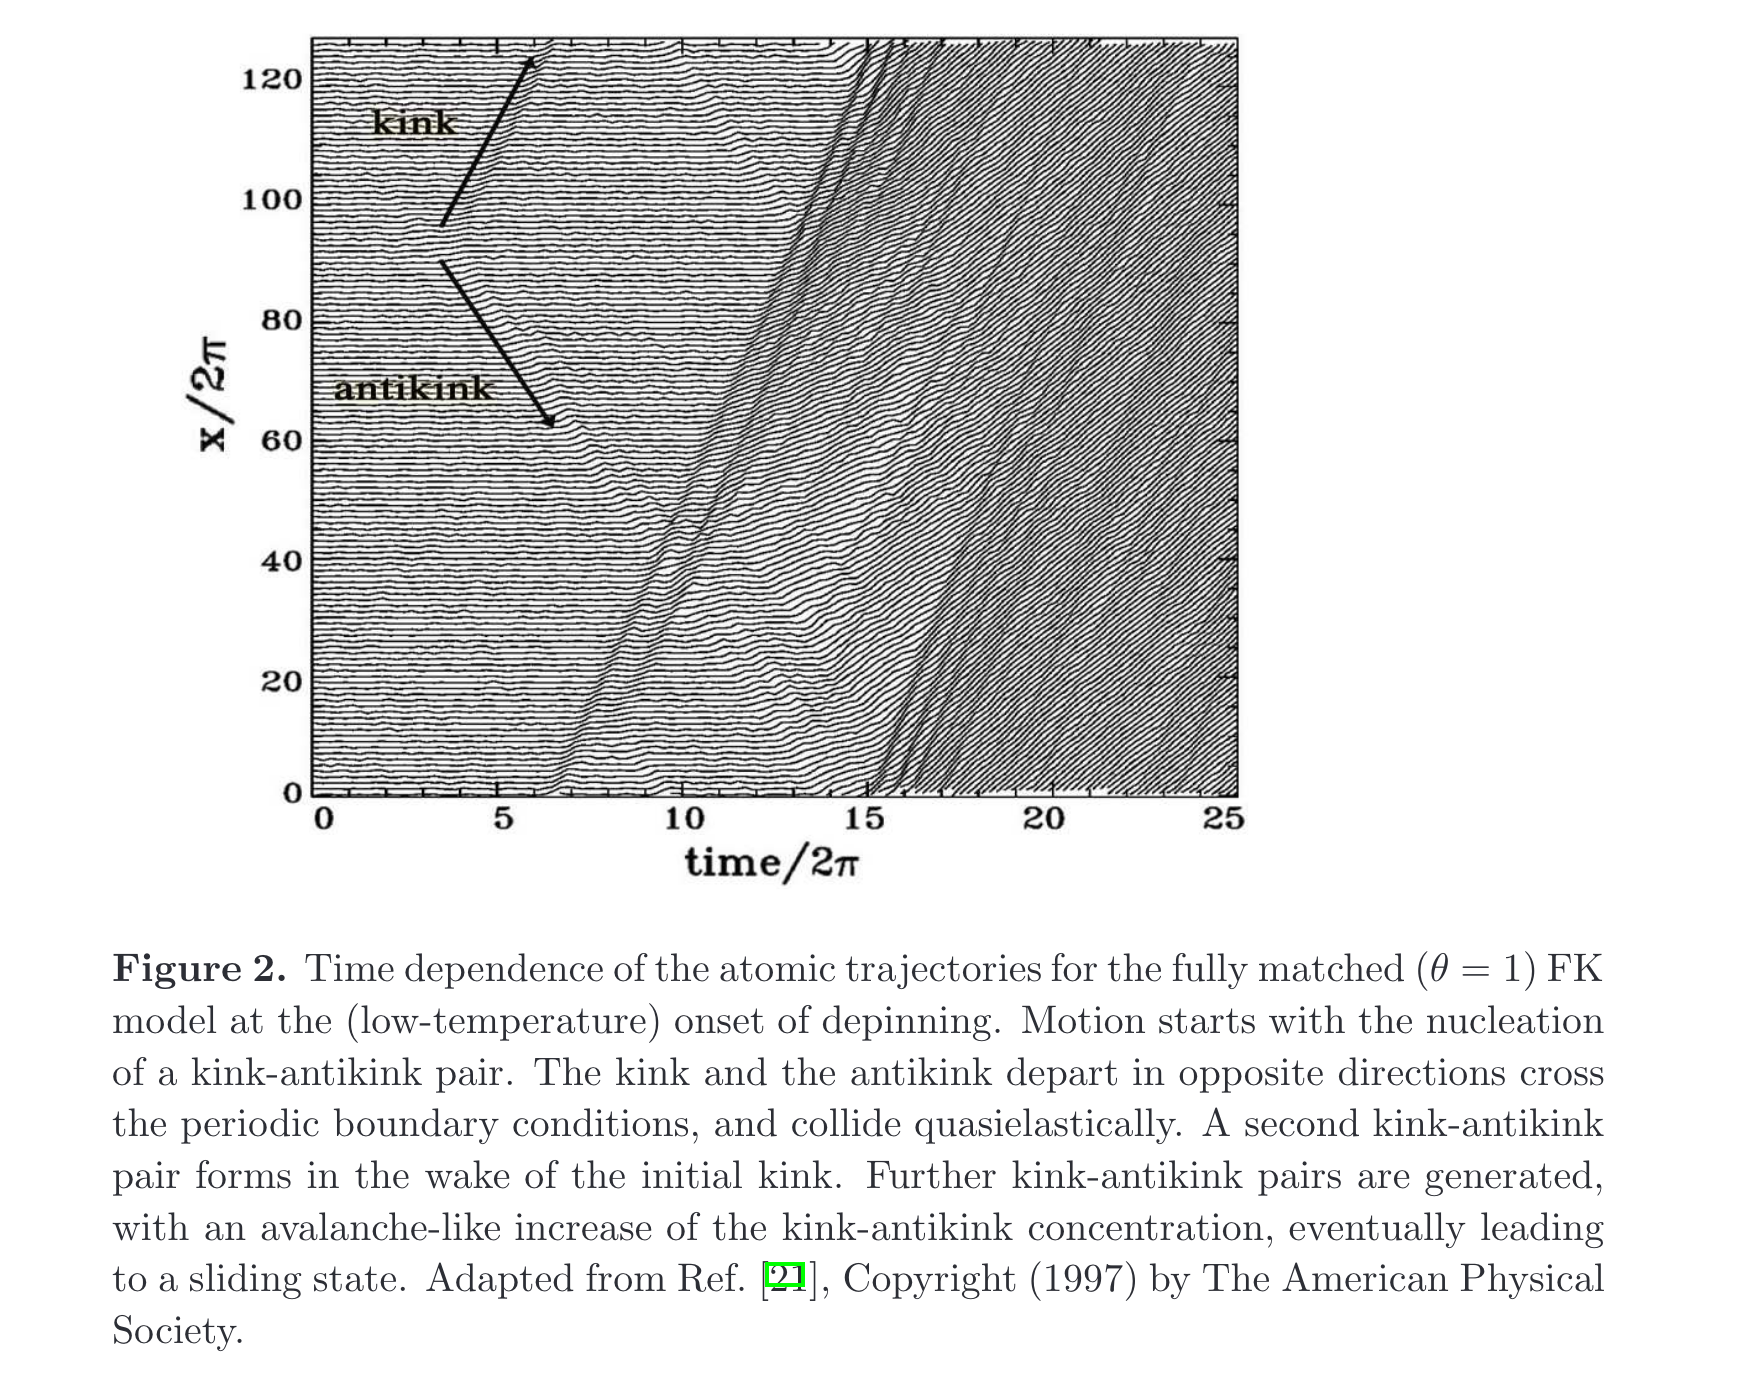
\includegraphics[width=0.45\linewidth]{figures/theory/kink_antikink.png}
  \caption{Detailed behavior (atomic trajectories vs time) at the depinning transition at a small nonzero temperature of the Frenkel-Kontorova chain with $\theta = 1$. The onset of motion is marked by the creation of one kink-antikink pair. The kink and antikink move in opposite directions, collide quasielastically (because of the periodic boundary conditions), and soon a second kink-antikink pair is created in the tail of the primary kink. This process repeats with an exponential (avalanchelike) growth of the kink-antikink concentration, leading to the totally sliding state. Adapted from~\cite{PhysRevLett.79.3692}, figure and caption reproduced from~\cite{Vanossi_2013} with permission from the American Physical Society.}
  \label{fig:kink_antikink}
\end{figure}


% where the chain is slightly compressed (expanded) to match the substrate potential, separated by kinks (antikinks), where the increased stress is eventually released.
% as illustrated in \cref{fig:incommensurable_example} 
% through a localized expansion (compression) 

% \hl{Go through this last part  again. Even though this is what the source says I'm not quite sure I understand why it is not opposite ``...released through a localized compression (expansion)''?}.


% Maybe use the strength $\lambda = U_0 / (K a_b^2)$ with critical strength $\lambda_c$ instead of critical $K$?

For the case of incommensurability, i.e.\ $\theta = a_b/a_c$ being irrational,
the \acrshort{GS} is characterized by a sort of ``staircase''  deformation. That
is, the chain will exhibit regular periods of regions with approximate
commensurability separated by regularly spaced kinks or antikinks. 


The incommensurable Frenkel-Kontorova model contains a critical elastic constant $K_c$, such that for $K > K_c$ the static friction $F_s$ drops to zero, making the chain able to initiate a slide at no energy cost, while the low-velocity kinetic friction is dramatically reduced. This can be explained by the
fact that the displacement occurring in the incommensurable case will yield just
as many atoms climbing up a corrugation as atoms climbing down. For a big (infinite) chain this will exactly balance the forces making it
non-resistant to sliding. Generally, incommensurability guarantees that the
total energy (at $T=0$) is independent of the relative position to the
potential. However, when sliding freely, a single atom will eventually occupy a
maximum of the potential, and thus when increasing the potential magnitude $U_0$ or
softening the chain stiffness, lowering $K$, the possibility to occupy such a
maximum disappears. This marks the so-called \text{aubry transition},
at the critical elastic constant $K = K_c(U_0, \theta)$, where the chain goes
from a free sliding to a \textit{pinned} state with nonzero static friction.
$K_c$ is a discontinuous function of the ratio $\theta$, due to the reliance on
irrational numbers for incommensurability. The minimal
value $K_c \simeq 1.0291926 $ in units $[2 U_0 (\pi / a_b)^2]$ is achieved for
the golden-mean ratio $\theta = (1+\sqrt{5}/2)$. The Aubry transition can be investigated as a first-order phase transition for which power laws can be defined for the order parameter, but this is beyond the scope of this thesis.


% The term superlubricity has been criticized as mislead-
% ing, since it might wrongly suggest zero friction in the sliding state in analogy to superconductivity and super- fluidity. Instead, incommensurability of periodic inter- faces cancels only one of the channels of energy dissipa- tion, that originating from the low-speed stick-slip insta- bility. Other dissipative processes, such as the emission of sound waves, still persist, and therefore even in the case of complete incommensurability the net kinetic friction force does not vanish. Nonetheless, in the superlubric regime one expects a substantial reduction of the friction force relative to a similar, but commensurate case.
% https://arxiv.org/abs/1112.3234v4


The phenomena of non-pinned configurations are named \textit{superlubricity} in
tribological context. Despite the misleading name, this refers to the case where
the static friction is zero while the kinetic friction is nonzero, but reduced.
For the case of a 2D sheet, it is possible to alter the commensurability, not
only by changing the lattice spacing through material choice but also by
changing the orientation of the sheet relative to the substrate. Dienwiebel et
al.~\cite{DIENWIEBEL2005197} have shown that the kinetic friction, for a
graphene flake sliding over a graphite surface (multiple layers of graphene),
exhibits extremely low friction at certain orientations as shown in
\cref{fig:graphene_rot}. As the orientation is changed they observed two spikes
of considerable friction while the remaining valleys correspond to effectively
zero friction in consideration of the measurement uncertainty. This phenomenon
relates to the transition between frictional regimes, as introduced through the
Prandtl–Tomlinson model, since the change in orientation affects the effective
substrate potential. Merely from the static consideration, we found that
lowering the potential amplitude $U_0$ will decrease the parameter $\eta =
2\pi^2U_0/a^2K$ shifting away from the regime of multiple slips towards smooth
sliding associated with low friction. Such transitions will also be affected by
the shape of the potential and corresponding 2D effects of the sliding
path~\cite{Yalin_2011}.

\begin{figure}[!htb]
  \centering
  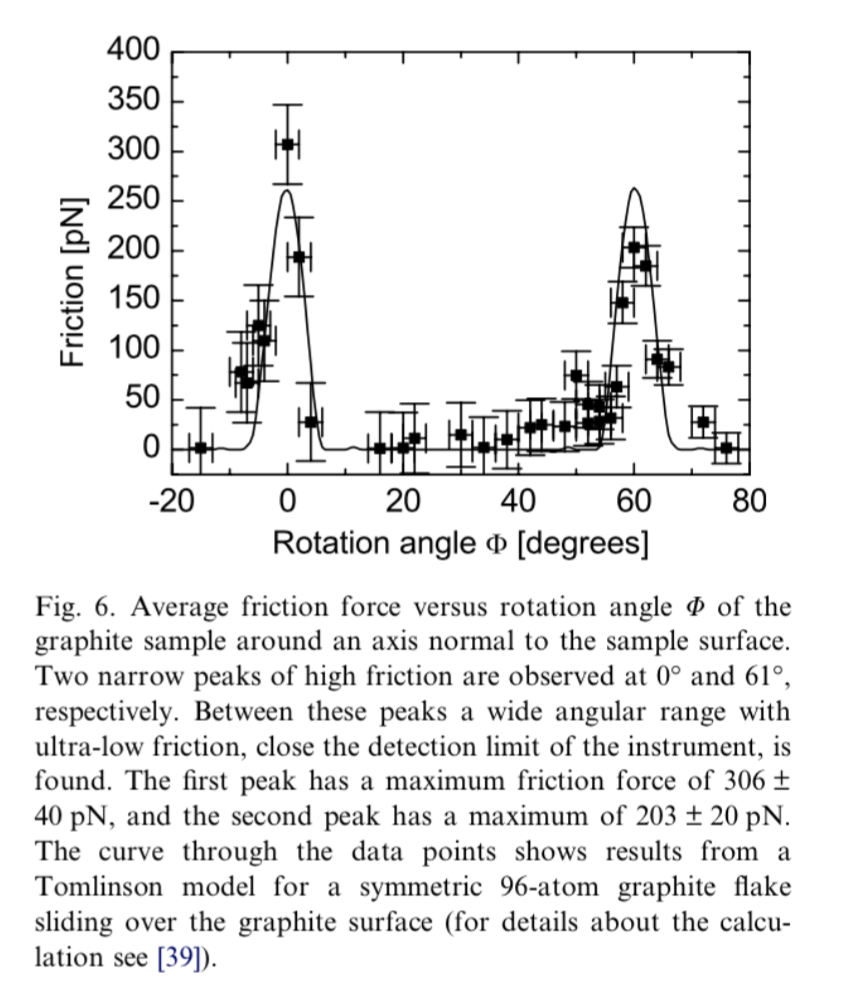
\includegraphics[width=0.55\linewidth]{figures/theory/graphene_rot.png}
  \caption{Average friction force versus rotation angle $\Phi$ of the
  graphite sample around an axis normal to the sample surface.
  Two narrow peaks of high friction are observed at 0$^{\circ}$ and 61$^{\circ}$,
  respectively. Between these peaks, a wide angular range with
  ultra-low friction, close to the detection limit of the instrument, is
  found. The first peak has a maximum friction force of $306 \pm \SI{40}{pN}$, and the second peak has a maximum of $203 \pm \SI{20}{pN}$.
  The curve through the data points shows results from a
  Tomlinson model for a symmetric 96-atom graphite flake
  sliding over the graphite surface (for details about the calculation see~\cite{PhysRevB.70.165418}). Figure and caption adapted from~\cite{DIENWIEBEL2005197}, reproduced from~\cite{Vanossi_2013} with permission from the American Physical Society.}
  \label{fig:graphene_rot}
\end{figure}






% The reason that friction lowers for incommensurability is 
% probably that we avoid stick-slip behavior which is highly 
% ``strongly dissipative stick-slip motion''~\cite{bonelli_atomistic_2009}


% Maybe check out for more info on the 1D model: Y. S. Kivshar O. M. Braun. The Frenkel-Kontorova Model. Springer, 1st edition, 2004.
% The Frenkel-Kontorova Model.pdf p. 38 3.2 Dynamics of Kinks <---------

%Based on~\cite{FK2D}


% The Frenkel-Kontorova model can also describe phonons and heat in the lattices, which absorb the kinetic energy of the sliding[4].~\cite{FK2D}

% Consequently, the Frenkel-Kontorova model is the simplest model in which dynamic friction is emergent, while in other models some form of heuristic damping must be included.\cite{FK2D}
\subsubsection{Velocity resosnance} % Velocity resosnance 
% The kinetic friction properties of the FK model (Strunz and Elmer, 1998a,b) are probed by adding a (e.g. Langevin) thermostat as described for the PT model above. Even where (above the Aubry transition) Fs = 0 the kinetic friction force Fk is nonzero, because the dy- namics at any finite speed results in the excitation of phonons in the chain.
% https://arxiv.org/abs/1112.3234v4

While many of the same arguments used for the Prandtl–Tomlinson model regarding velocity dependence for friction can be made for the Frenkel-Kontorova model, the addition of multiple atoms introduces the possibility of resonance. In the Frenkel-Kontorova model, the kinetic friction is primarily attributed to resonance between the sliding-induced vibrations and phonon modes in the chain~\cite{FK2D}. The specific dynamics are found to be highly model and dimension specific, and even for the 1D case, this is rather complex. However, we make a simplified analysis of the 1D rigid chain in order to showcase the reasoning behind the phenomena.

When all atoms are sliding rigidly with center of mass (\acrshort{CM}) velocity $v_{{\text{CM}}}$ the atoms will pass the potential maxima with the so-called \textit{washboard frequency} $\Omega = 2\pi v_{{\text{CM}}} / a_b$. For a weak coupling between the chain and the potential we can use the zero potential case as an approximation for which the known dispersion relation for the 1D harmonic chain is given~\cite[p. 92]{Kittel2004}
\begin{align*}
  \omega_k = \sqrt{\frac{4 K}{m}} \left|\sin{\left(\frac{k}{2}\right)}\right|,
\end{align*}
where $\omega_k$ is the phonon frequency and $k = 2\pi i / N$ the wavenumber with $i\in [N/2, N/2)$. Resonance will occur when the washboard frequency $\Omega$ is close to the frequency of the phonon modes $\omega_q$ in the chain with wavenumber $q = 2\pi a_c / a_b = 2\pi \theta^{-1}$ or its harmonics $nq$ for $n = 1, 2, 3, \hdots$~\cite{van_den_Ende_2012}. Thus, we can approximate the resonance \acrshort{CM} speed as
\begin{align*}
    n \Omega &\sim \omega_{nq} \\
    n \frac{2\pi v_{\text{CM}}}{a_b} &\sim \sqrt{\frac{4K}{m}} \left| \sin{\left(\frac{2n \pi \theta^{-1}}{2}\right)}\right| \\
    v_{\text{CM}} &\sim \frac{\sin{(n\pi \theta^{-1})}}{n \pi} \sqrt{\frac{Ka_b^2}{m}}.
\end{align*}
When the chain slides with a velocity around resonance speed, the washboard
frequency can excite acoustic phonons which will dissipate to other phonon modes
as well. At zero temperature, the energy will transform back and forth between
internal degrees of freedom and \acrshort{CM} movement of the chain. Without any dissipation mechanism, this is theorized to speed up the translational decay~\cite{FK2D}. However, as soon as we add a dissipation channel through the substrate, energy will dissipate from the chain to the substrate's degrees of freedom. This suggests that certain sliding speeds will exhibit relatively high kinetic friction while
others will be subject to relatively low kinetic friction. Simulations of
concentric nanotubes in relative motion (telescopic sliding) support this idea
as it has revealed the occurrence of certain velocities at which the friction is
enhanced, corresponding to the washboard frequency of the
system~\cite{Zhang_2007, Zhang_2009}. The friction response was observed to be highly non-linear as the resonance velocities were approached. 

The analysis of the phonon dynamics is highly simplified here, and a numerical study of the Frenkel-Kontorova by Norell et al.~\cite{FK2D} showed that the behavior was highly dependent on model parameter choices, but that the friction generally increased with velocity and temperature. Here the latter observation differs qualitatively from that of the Prandtl–Tomlinson model.



% This is strongly connected to the superlubricity term, although the phonon
% dynamics in this analysis is overly simplified, and additionaly we expect more
% complex resonance dynamics for higher dimensions. 


% A common way to model the non-zero temperature case is by the use of a Langevin
% thermostat, which models the dissipation of heat by adding a viscous damping
% force and thermal fluctuations by the addition of Gaussian random forces with
% variance proportional to the temperature (see \cref{sec:langevin} for more details). In combination, this gives rise to a kinetic
% friction that is both velocity and temperature dependent. By extending the Frenkel-Kontorova model into 2D~\cite{FK2D} it can be shown numerically that
% the friction coefficient generally increases with increasing velocity and
% temperature resepectively, although the specific of the trend is highly
% sensitive to model parameters. 




% As the system is Hamiltonian (no heuristic damping) the total energy is conserved. Nevertheless, energy can be transferred from the centre of mass to the internal degrees of freedom, leading to the arrest of the chain in time. This effect can be interpreted as an effective friction.~\cite{van_den_Ende_2012}


% The majority [6–12] examines the steady state of the dynamical Frenkel-Kontorova model in the presence of dissipation, rep- resenting the coupling of phonons to other, undescribed degrees of freedom.~\cite{PhysRevLett.85.302}


% Static friciton behvaiour is robust and remains similar in 2D but dynamical friction is strongly influenced. 




% When considering the nonzero temperature thermal fluctuations can then overcome pinning effects even in fully commensurate cases.



% By applying a finite driving force it is known that a pinned configuration will go through several first-order dynamical pahse transitions as the system transfers from a pinned to a sliding state. 



% At face value, the transition from a static strained configuration to full
% sliding is conceptually as simple as overcoming an energy barrier. However,
% practical single- and multiple- contact conditions are characterized by
% complex interaction profiles plus nontrivial internal dynamics. As a result,
% the interplay of thermal drifts, contact ageing, contact-contact in-
% teractions, and macroscopic elastic deformations introduce significant
% complications, and make the depinning transition from static to kinetic
% friction an active field of research. The depinning dynamics affects in
% particular the transition between stick-slip and smooth slid- ing for sliding
% friction. (Current trends in the physics of nanoscale friction)


% In Atomic Force Microscopy (AFM) experiments, when the tip scans over the
% monolayers at low speeds, friction force is reported to increase with the
% logarithm of the velocity, similar to that observed when the tip scans across
% crystalline surfaces. This velocity dependence is interpreted in terms of
% thermally activated depinning of interlocking barriers involving interfacial
% atoms. (Current trends in the physics of nanoscale friction)






% "However, it is well known that continuum mechanics is valid only when the dimensions of the studied object are much larger than the length scale of the atomic disconti- nuity. Therefore, when the scale of the single asperity is on the order of nanometers, the effect of the discontinuity of the atoms within the tip and substrate can no longer be neglected [47]. Recent AFM experiments on metals revealed that friction varies little with increase of normal load in the low load regime [24, 74]. In addition, a newly invented AFM technique referred to as tip-on-top mode that enables researchers to manipulate nanoparticles of different size showed that in some cases friction increased linearly with interface area while in other cases near fric- tionless sliding was observed [75]. These conflicting results suggest that there may be a non-linear relationship between real contact area and friction."~\cite{Yalin_2011}


% The essential difference between the FK and FKT models is that only the end atom is attached to the support in FK while all atoms are attached to the support in FKT.~\cite{Yalin_2011}


% The friction comes from the viscous force which is proportional to sliding speed. Physically speaking, the viscous term is due to phonon excitation. So the term ‘‘superlubricity’’ which suggests cancelation of friction to zero may not be appropriate; structural lubricity proposed by Mu ̈ser is a better term to describe the phenomenon [77].~\cite{Yalin_2011}



\subsection{Frenkel-Kontorova-Tomlinson}
A final extension of the atomic models worth mentioning here is the
Frenkel-Kontorova-Tomlinson (\acrshort{FKT}) model~\cite{weiss_dry_1997}, which
introduces a harmonic coupling of the sliding atom chain to the moving body,
effectively combining Prandtl–Tomlinson and Frenkel-Kontorova
(see~\cref{fig:PT_FK_FKT}). This introduces more degrees of freedom to the model
which is based on the intention of getting a more realistic connection between
the moving body and the chain. Dong et al.~\cite{Yalin_2011} carried out a numerical analysis
using the 1D Frenkel-Kontorova-Tomlinson model to investigate the effect of
chain length. They observed that the friction increased linearly with the number
of atoms in the chain on a long range, but certain lattice mismatches resulted in
local non-linear relationships as shown in~\cref{fig:FKT_contact}. Similarly, by
extending the Frenkel-Kontorova-Tomlinson model to 2D they were able to achieve
a similar sensitivity to commensurability as observed experimentally
by~\cite{DIENWIEBEL2005197} (see~\cref{fig:graphene_rot}) with the numerical
result shown in~\cref{fig:FKT_2D_rot}. Besides a demonstration of the
commensurability effect in 2D they also observed increasing friction with an
increasing flake size. Combined, the 1D and 2D results support the idea of
increasing friction with contact size although it might showcase non-linear
behavior depending on commensurability.


\begin{figure}[!htb]
  \centering
  \begin{subfigure}[t]{0.49\textwidth}
      \centering
      \includegraphics[width=\textwidth]{figures/theory/FKT_contact.png}
      \label{fig:FKT_contact}
  \end{subfigure}
  \hfill
  \begin{subfigure}[t]{0.49\textwidth}
      \centering
      \includegraphics[width=\textwidth]{figures/theory/FKT_2D_rot.png}
      \label{fig:FKT_2D_rot}
    \end{subfigure}
    \hfill
     \caption{Friction in the Frenkel-Kontorova-Tomlinson model for varying size and Commensurability corresponding to numerical result by Dong et al.~\cite{Yalin_2011}. $K_t$ describes the interatomic spring constant and $K$ the coupling to the moving body. (a) The 1D case with an increasing number of atoms in the chain and different mismatch length ratios $\theta = a_b / a_c$, given as $a/b$ in their notation. The model parameters are $K = \SI{5}{N/m}$, $K_t = \SI{50}{N/m}$. (b) The 2D case with varying angles (misfit angle) between the flake and the substrate. The model parameters are $K = \SI{10}{N/m}$, $K_t = \SI{50}{N/m}$. Reproduced from~\cite{Yalin_2011}.}
     \label{fig:FKT_size}
\end{figure}


\subsection{Shortcomings of reduced-models}
It should be noted that the reduced-models presented in this work provide a simplified description of the friction behavior. One major limitation is that all models assume a rigid substrate with a sinusoidal potential shape, whereas in reality, the substrate reaction to sliding motion results in a constantly changing potential, making the dynamics more intricate. Moreover, the energy dissipation is simplified through a viscous term $-m\mu \dot{x}$ in the Langevin equations~\cref{eq:Langevin_PT}, which neglects the complexity associated with electron and phonon dissipation. For example, considering phonon dissipation, there exist many vibration modes ($3N$), and thus many dissipation channels for the tip. Lastly, it should be mentioned that the moving body is simplified as a constantly moving rigid body, whereas in reality, it may exhibit a more complicated dynamic behavior.


% On a final note, we point out that the reduced-models describe the friction behavior in a highly simplified manner. Some shortcomings include the fact that they assume a rigid substrate with a simple sinusoidal potential shape. In reality, the substrate reaction to sliding motion will make for a changing potential throughout the simulation which makes the dynamics more complex. Similarly, the energy dissipation is simplified through a viscous term $-m\mu \dot{x}$ from the Langevin equations \cref{eq:Langevin_PT}. This does not capture the full complexity associated with electron and phonon dissipation~\cite{Yalin_2011}. Taking phonon dissipation as an example there are $3N$ vibration modes, and thus many dissipation channels for the tip. Finally, we also point out that the moving body is simplified as a constantly moving rigid body, while in reality, this might also be subject to more complex dynamic behavior.



% \hl{To-DO: Shortcomings of PT-based reduced-models} %~\cite{Yalin_2011}. 
% \begin{itemize}
%   \item Assumes a rigid substrate with a simplified potential shape. 
%   \item Energy dissipation is added through a viscous term $-m\mu \dot{x}$ being the only dissipation channel availble. Does not capture a more complex real-life electron and phonon dissipation. Taking phonon dissipation as an example there are many vibration modes (3N). This will affect the thermal activation derivation. 
%   \item The moving body is simplified as a constantly moving rigid body, while in fact this will also be subject to a more complex dynamic behavior.
% \end{itemize}


% However, Weiss and Elmer (1995) proposed that the model had a deficiency. They suggested that in the FK model, there was no connection between the atoms and the sliding body. Therefore, Frenkel-Kontorova-Tomlinson (FKT) model that combines the FK model with the Tomlinson model was proposed.~\cite{kim_nano-scale_2009}


% The Frenkel-Kontorova-Tomlinson (FKT) model [61, 62] introduces an harmonic
% coupling of the sliding atomic chain to a driving moving body, thus making it
% possible to investigate stick-slip features in a 1D extended simplified
% contact. The FKT framework provided the ideal platform to investigate the
% tribological consequences of combined interface incommensurability,
% finite-size effects, mechanical stiffness of the contacting materials, and
% normal-load variations~\cite{Manini_2016}.


% Important generalizations involving increased dimensionality compared to the
% regular FK model bear significant implications for tribological properties
% such as critical exponents, size-scaling of the friction force, depinning
% mechanisms, and others.~\cite{Manini_2016}

% Maybe check this out: An interesting example of such a transient is the
% depinning of an atomic monolayer driven across a 2D periodic substrate profile
% of hexagonal symmetry [83]. ~\cite{Manini_2016}


% \subsection{Other stuff}


% At nanoscales things get a bit more unclear. SFM (explain) experiments have
% reported (copy sources 5, 6, 21 from~\cite{mo_friction_2009}) where $F_f \propto
% F_N$ or even with these quantities being nearly independent of each other.

%~\cite{physicsworld_2005}

% Physically relevant quantities, including the average friction force, the slider and the lubricant mean velocities, several correlation functions, and the heat flow can be evaluated numerically by carrying out suitable averages over the model dynamics of a sliding interface, as long as it is followed for a sufficiently long time. The modeling of friction must first of all address correctly ordinary equilibrium and near-equilibrium phenomena, where the fluctuation-dissipation theorem (Sec. 2) governs the smooth conversion of mechanical energy into heat, but most importantly it must also deal with inherently nonlinear dissipative phenomena such as instabilities, stick-slip, and all kinds of hysteretic response to external driving forces, characteristic of non-equilibrium dynamics. 
%~\cite{Manini_2016}


% In several works by J. Fineberg’s group [2–4] the transition from sticking to
% sliding is characterized by slip fronts propagating along the interface.
%~\cite{Manini_2017}[p. 2]. 



% As expected, high levels of
% friction were present in the commensurate positions and extremely low friction
% was found when the surfaces were incommensurate.
% (\url{https://physicsworld.com/a/friction-at-the-nano-scale/})


% Superlubricity, now a pervasive concept of
% modern tribology, dates back to the math- ematical framework of the Frenkel
% Kontorova model for incommensurate interfaces [40]. When two contacting
% crystalline workpieces are out of registry, by lattice mismatch or angular
% misalignment, the minimal force required to achieve sliding, i.e. the static
% friction, tends to zero in the thermodynamic limit – that is, it can at most
% grow as a power less than one of the area – provided the two substrates are
% stiff enough. (Current trends in the physics of nanoscale friction)


% Superlubricity is experimentally rare. Until recently, it has been
% demonstrated or im- plied in a relatively small number of cases [29, 42–46].
% There are now more evidences of superlubric behavior in cluster
% nanomanipulation [32, 33, 47], sliding colloidal layers [48–50], and
% inertially driven rare-gas adsorbates [51, 52]. (Current trends in the physics
% of nanoscale friction)


% A breakdown of structural lubricity may occur at the heterogeneous interface
% of graphene and h-BN. Because of lattice mismatch (1.8\%), this interface is
% intrinsically incommen- surate, and superlubricity should persist regardless
% of the flake-substrate orientation, and become more and more evident as the
% flake size increases [57]. However, vertical cor- rugations and planar strains
% may occur at the interface even in the presence of weak van der Waals
% interactions and, since the lattice mismatch is small, the system can de-
% velop locally commensurate and incommensurate domains as a function of the
% misfit angle [58, 59]. Nonetheless, spontaneous rotation of large graphene
% flakes on h-BN is observed after thermal annealing at elevated temperatures,
% indicative of very low friction due to incommensurate sliding [60, 61].
% (Current trends in the physics of nanoscale friction)

% Indeed, we know from theory and simulation [74–76] that even in clean wearless
% friction experiments with perfect atomic structures, superlubricity at large
% scales may, for example, surrender due to the soft elastic strain deformations
% of contacting systems. (Current trends in the physics of nanoscale friction)



% \section{Multi scale models?}
%~\cite{Manini_2016} p. 24.


% Might find something interesting here~\cite{zhao_thermally_2007} or~\cite{PhysRevE.71.065101}.

% Find a suitable place to introduce smooth sliding. Above certain velocities the stick-slip motion dissapear.~\cite[p. 142-ish]{gnecco_meyer_2015}

\subsection{Experimental procedures}
%~\cite{gnecco_meyer_2015}
% Check out this~\cite{Dong_2013} parameter choices for MD

Experimentally, the study of nanoscale friction is challenging due to the low
forces on the scale of nano-newtons along with the difficulties of mapping the
nano-scale topography of the sample. In contrast to numerical simulations, which provide full
transparency regarding atomic-scale structures, sampling of forces, velocities
and temperature, the experimental results are limited by the state-of-the-art
experimental methods. To facilitate the comparison of numerical and experimental results, we will address a few of the most relevant experimental methods.


\subsubsection{Scanning Probe Microscopy}\label{sec:SPM} 
Scanning probe microscopy (\acrshort{SPM}) includes a variety of experimental
methods which are used to examine surfaces with atomic resolution~\cite[pp.
6--27]{BHUSHAN20051507}. This was originally developed for surface topography
imaging, but today it plays a crucial role in nanoscale science as it is used
for probe-sampling regarding tribological, electronic, magnetic, biological and
chemical character. The family of methods involving the measurement of forces is
generally referred to as \textit{scanning force microscopy} (\acrshort{SFM})
or for friction purposes \textit{friction force microscopy} (\acrshort{FFM}).

One such method arose from the \textit{atomic force microscope} \acrshort{AFM}, which consists of a sharp micro-fabricated tip attached to a cantilever force sensor, usually with a sensitivity below \SI{1}{nN} all the way down to pN. The force is measured by recording the bending of
the cantilever, either as a change in electrical conduction or more commonly, by
a light beam reflected from the back of the cantilever into a photodetector~\cite[p. 183]{gnecco_meyer_2015} as shown in~\cref{fig:AFM}. By adjusting the tip-sample height to keep a constant normal force while scanning across the surface, the \acrshort{AFM} can be used to produce a
surface topography map.  However, when scanning perpendicularly to the cantilever axis, the frictional force can be measured as the torsion of the cantilever. By utilizing a photodetector with four quadrants (as depicted in~\cref{fig:AFM}), the normal force and friction force can be simultaneously measured as the probes scan across the surface. However, when scanning
perpendicularly to the cantilever axis, one is also able to measure the
frictional force as torsion of the cantilever. By having four quadrants in the
photodetector (see~\cref{fig:AFM}), one can simultaneously
measure the normal force and friction force as the probes scan across the
surface. \acrshort{AFM} can also be utilized to drag a nanoflake across the substrate, as demonstrated by Dienwiebel et al.~\cite{DIENWIEBEL2005197}, who attached a graphene flake to a \acrshort{AFM} tip and dragged it across graphite. However, it should be noted that this method concentrates the normal loading to a single point on the flake, rather than achieving an evenly distributed load.


\subsubsection{Surface Force Apparatus}
Finally, it is worth mentioning the Surface Force Apparatus (\acrshort{SFA}), which consists of two curved, molecularly smooth surfaces brought into contact~\cite[p. 188]{gnecco_meyer_2015}. The material of choice is usually mica since it can be easily cleaved into atomically flat surfaces over macroscopic areas. The sample is then placed between the two surfaces as a lubricant film, and the friction properties can be studied by applying a tangential force to the surfaces.

\begin{figure}[!htb]
  \centering
  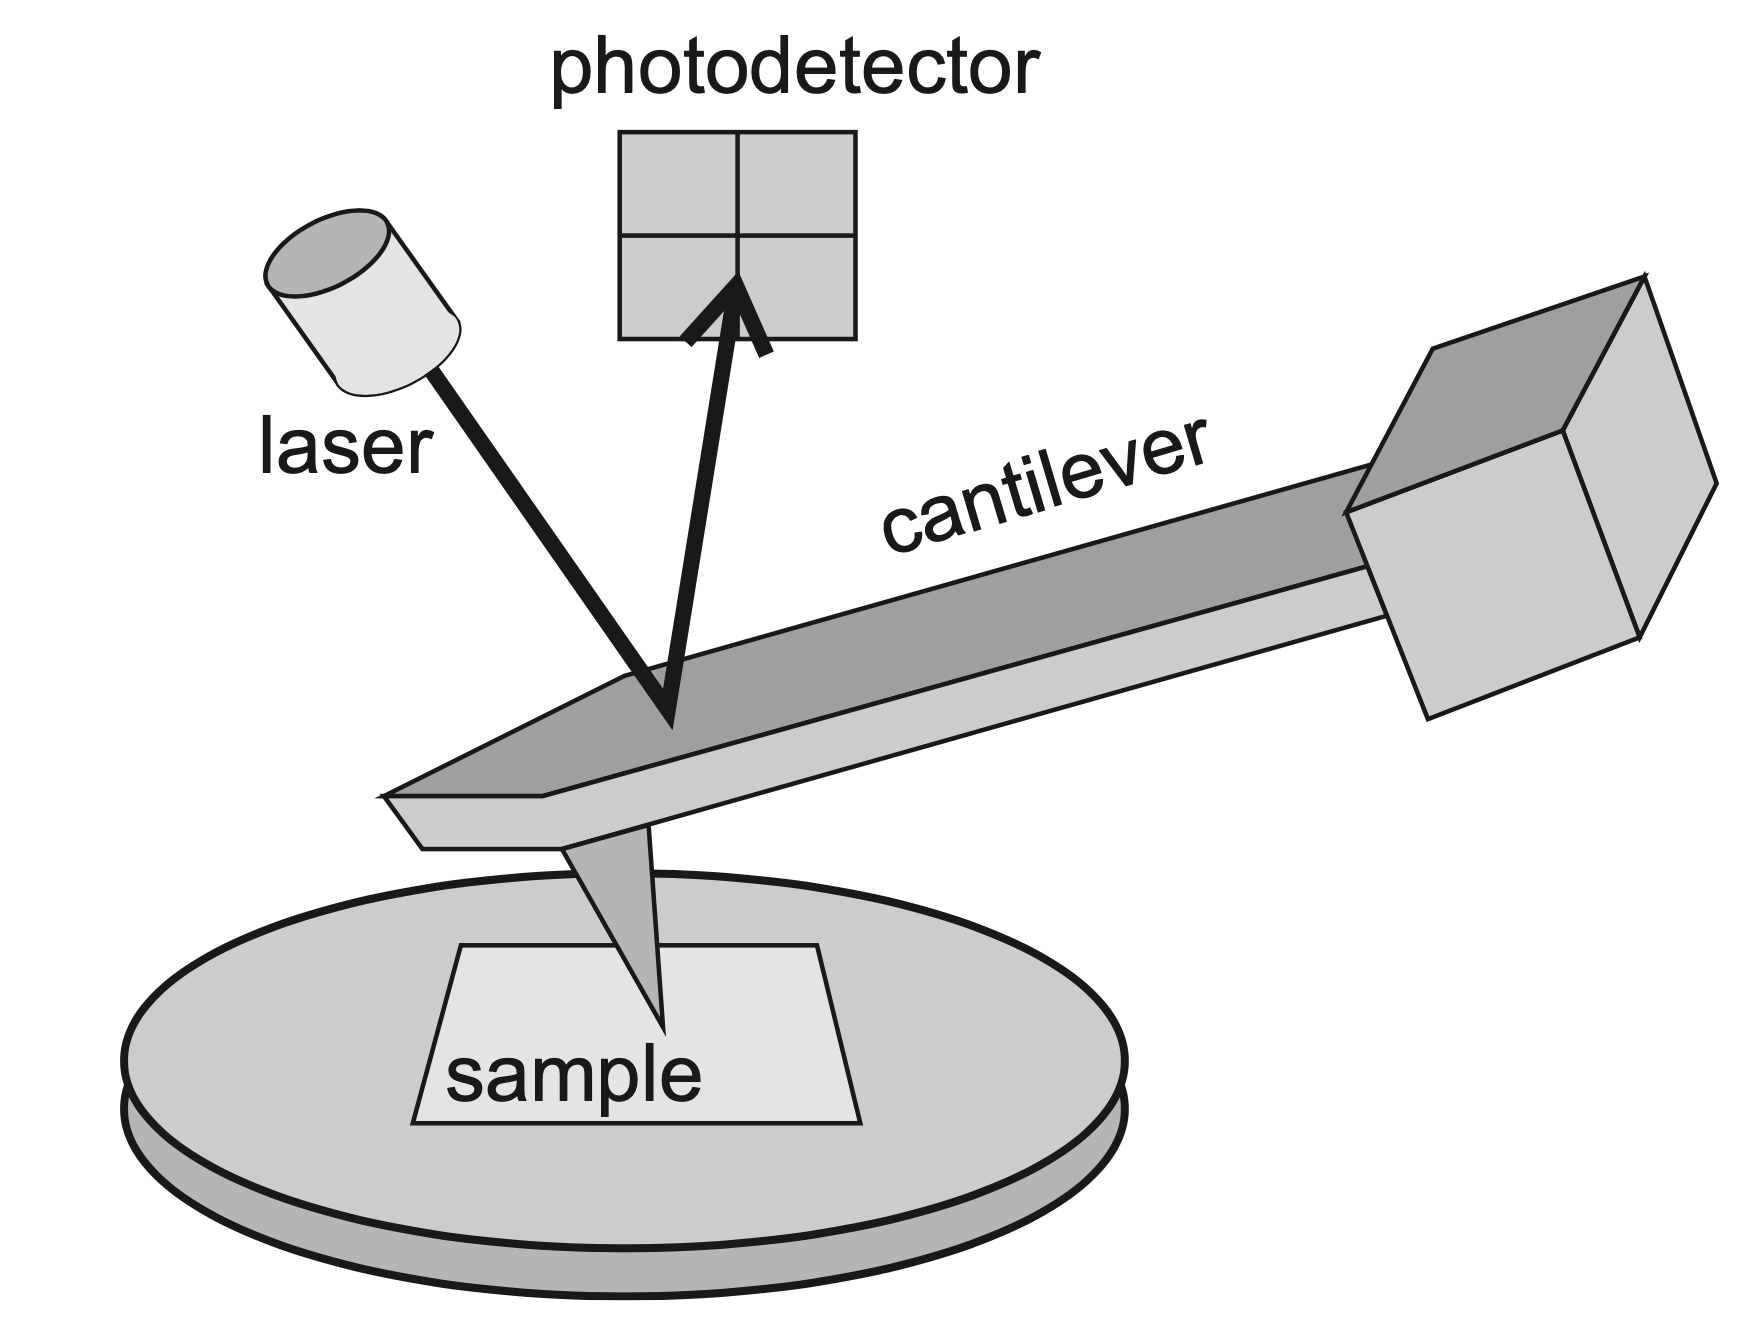
\includegraphics[width=0.5\linewidth]{figures/theory/AFM.png}
  \caption{Schematic diagram of a beam-deflection atomic force microscope. Figure and caption reproduced from~\cite[p. 184]{gnecco_meyer_2015}.}
  \label{fig:AFM}
\end{figure}



\section{Summary of previous results}\label{sec:prev_results}
Several studies have investigated the frictional behavior of graphene by varying
different parameters such as normal force, sliding velocity, temperature,
commensurability and graphene thickness~\cite{penkov_tribology_2014}. In
general, we find three types of relevant systems being studied: 1) An
\acrshort{FFM}-type setup where the graphene, either resting on a substrate or
suspended, is probed by an \acrshort{AFM} tip scanning across the surface. 2) A
\acrshort{SFA} setup with the graphene ``sandwiched'' in between two substrate
layers moving relative to each other using the graphene as a solid lubricant. 3)
A graphene flake sliding on a substrate, either being dragged by an
\acrshort{AFM} tip or by a more complex arrangement in numerical simulations.
Considering that even the sharpest \acrshort{AFM} tip will effectively put
multiple atoms in contact with the sample, all methods are relatable to the
study of nanoscale surface contacts. However, the \acrshort{FFM}-type is more
closely related to asperity theory since it is expected to deform under
increasing load, while the latter two are more aligned with the
Prandtl–Tomlinson type models and our specific system of interest. Nonetheless,
we will consider results across all three types of systems. The majority of the studies considers are summarized in~\cref{tab:friction_ref} for convenience. 


\begin{table}[!htb]
  % \begin{center}
  \centering
  \caption{A summary of the main studies considered for the review of previous results in~\cref{sec:prev_results}. The table provides a distinction between the different types of systems in the study: \acrshort{FFM}, \acrshort{SFA} or flake on a substrate, as well as whether they were numerically (num.) or experimentally.}
  \label{tab:friction_ref}
  \begin{tabular}{ |M{1cm}|M{1cm}|M{1.5cm}|X{2.5cm}|X{4cm}|X{4cm}| } \hline
  System & Type & Year & Researcher & Materials & Keywords \\ \hline
  \parbox[t]{2mm}{\multirow{10}{*}{\rotatebox[origin=c]{90}{\acrshort{FFM}}}} & \multirow{3}{*}{Exp.} & 2007~\cite{zhao_thermally_2007} & Zhao et al.\ & Si\textsubscript{3}N\textsubscript{4} tip on graphite. & Temperature dependence. \\ \cline{3-6} 
  & & 2015~\cite{Paolicelli_2015} & G. Paolicelli et al.\ & Si tip, graphene on SiO2 and Ni(111) substrate  &  Load, environment, graphene layers. \\ \cline{2-6} 
  & Both & 2019~\cite{zhang_tuning_2019} & Zhang et al.\ & Monolayer graphene  & Straining of graphene sheet. \\ \cline{2-6} 
  & \multirow{3}{*}{Num.} & 2015~\cite{Yoon2015MolecularDS} & Yoon et al.\ & Si tip, graphene on SiO\textsubscript{2} & Stick-slip: tip size, scan angle, layer thickness, substrate flexibility. \\ \cline{3-6} 
  & & 2016~\cite{li_evolving_2016} & Li et al.\ & Si tip, graphene on a-Si substrate & Graphene layers, friction strengthening, stick-slip \\ \cline{1-6} 
  \parbox[t]{2mm}{\multirow{3}{*}{\rotatebox[origin=c]{90}{\acrshort{SFA}}}} & \multirow{3}{*}{Num.} & 2011~\cite{Wijn_2011} & Wijn et al.\ & Graphene flakes between graphite  & Commensurability, rotational dynamics, superlubricity, temperature.  \\ \cline{3-6} 
  & & 2012~\cite{Kim_2012} & H.\ J.\ Kim and D.\ E.\ Kim. & Carbon sheet  & Corrugated nano-structured surfaces  \\ \cline{1-6} 
  \parbox[t]{2mm}{\multirow{18}{*}{\rotatebox[origin=c]{90}{Flake}}} & \multirow{5}{*}{Exp.} & 2005~\cite{DIENWIEBEL2005197} & Dienwiebel et al.\ & Graphene on graphite & Commensurability, superlubricity, load.  \\ \cline{3-6} 
  &  & 2013~\cite{feng_superlubric_2013}  & Feng et al.\ & Graphene on graphite &  Commensurability, superlubricity, temperature.  \\ \cline{2-6} 
  & \multirow{13}{*}{Num.} & 2009~\cite{bonelli_atomistic_2009} & Bonelli et al.\ & Graphene on graphite  & Tight-binding, commensurability, load, flake size. \\ \cline{3-6} 
  &  & 2012~\cite{Reguzzoni_2012} & Reguzzoni et al.\ & Graphene on graphite & Graphite layers. \\ \cline{3-6} 
  &  & 2014~\cite{liu_high-speed_2014} & Liu et al.\ & Graphene on graphite & High speed, superlubricity, rotational dynamics, sheet strain. \\ \cline{3-6} 
  &  & 2018~\cite{zhu_study_2018} & P. Zhu and Li & Graphene on gold & Stick-slip, commensurability, flake size and shape. \\ \cline{3-6} 
  &  & 2019~\cite{ma12091425} & Zhang et al.\  & Graphene on diamond & Temperature, commensurability, friction coefficient.  \\ \cline{1-6} 
\end{tabular}
% \end{center}
\end{table}
% &  & 2019~\cite{Vazirisereshk_2019} & Vazirisereshk et al.\ & Graphene,  MoS\textsubscript{2} and Graphene/MoS\textsubscript{2} heterostructure & Low friction? \\ \cline{2-6} 


% Prandtl–Tomlinson model (\acrshort{PT})
% Frenkel-Kontorova-Tomlinson (\acrshort{FKT})

% Stick-slip
One of the earliest tribological simulations of graphene was carried out by
Bonelli et al.~\cite{bonelli_atomistic_2009} in 2009 using a tight-binding\footnote{The tight-binding method involves computing the electronic structure of the system, but it uses a semi-empirical approach to reduce the computational cost of those calculations. Thus, this method lies between traditional \acrshort{MD} and more expensive ab initio methods~\cite{colombo_tight-binding_2005}.} method (excluding thermal excitations) to simulate a graphene flake on an
infinite graphene sheet~\cite{penkov_tribology_2014}. They implemented a
Frenkel-Kontorova-Tomlinson-like setup where each atom in the flake is coupled horizontally
to a rigid support by elastic springs. They recovered the stick-slip behavior,
which is also observed in \acrshort{FFM} setups both experimentally~\cite{zhao_thermally_2007, zhang_tuning_2019} and numerically~\cite{li_evolving_2016, zhu_study_2018}. Moreover, they found an agreement with
the qualitative observation that soft springs allow for a clean stick-slip
motion while hard springs ($\sim \SI{40}{N/m}$) inhibited it, which also aligns
with the Prandtl–Tomlinson model. In \acrshort{AFM} and \acrshort{SFA} experiments,
the stick-slip motion tends to transition into smooth sliding when the speed
exceeds $\sim \SI{1}{\mu/s}$ while in \acrshort{MD} modeling the same transition
is observed in the $\sim \SI{1}{m/s}$ region~\cite{Manini_2016}. More precisely
Liu et al.~\cite{liu_high-speed_2014} finds this transition in \acrshort{MD}
simulations at \SI{15}{m/s}. This 6-order-of-magnitude discrepancy has been
largely discussed in connection to simplifying assumptions in \acrshort{MD}
simulations. On the other hand, the Prandtl–Tomlinson model qualitatively disagrees
as it predicts smooth sliding for low speeds only.
However, in an extension of the Prandtl–Tomlinson for the study of nanoscale rolling friction by Sircar and Patra~\cite{Sircar_2020}, they found smooth sliding for high speeds as well.


% Commensurability
Bonelli et al.~\cite{bonelli_atomistic_2009} also found that commensurability,
through orientation of the flake and the direction of sliding, had a great
impact on the frictional behavior which generally aligns with the predictions of
the Frenkel-Kontorova models. They confirmed qualitatively the
observation of superlubricity for certain incommensurable orientations which has
been reported in experiments by Dienwiebel et al.\cite{DIENWIEBEL2005197} and
further supported by experimental measurements of interaction energies by Feng
et al.~\cite{feng_superlubric_2013}. The importance of commensurability is also
reported for \acrshort{MD} simulations~\cite{ma12091425, zhu_study_2018,
Wijn_2011}. Bonelli et al.\ found the friction force and coefficient to be one
order of magnitude higher than that of the experimental results which they
attribute to the details of the numerical modeling. Generally, the experimental
coefficients between graphite and most materials lie in the range of 0.08--0.18~\cite{DIENWIEBEL2005197}. While Dienwiebel et al.~\cite{DIENWIEBEL2005197}
reported a wide range of frictional forces from $28 \pm \SI{16}{pN}$ to $453 \pm \SI{16}{pN}$ with loads $\sim [-10, 20]$ nN, the change in friction with applied load was
as low as 0.05--0.4\% for the incommensurable orientations. When using the slope definition for the frictional coefficient (\cref{eq:mu_def2}), this corresponds to a coefficient in the range of 0.0005--0.004. Bonelli et al.\ attribute the low dependency to a lacking change in contact area as the flake is loaded. 

% Flake size
Furthermore, Bonelli et al.~\cite{bonelli_atomistic_2009} found friction to
decrease with increasing flake size which is also reported in \acrshort{MD}
simulations for graphene on gold~\cite{zhu_study_2018}. Bonelli et al.\ mainly
attribute this to boundary effects, but also note that the coupling to the
support made for decreased rotational freedom as flake size was increased. Thus,
they hypothesized that the decreased freedom led to the graphene taking a more
forced path which is associated with a decreased stick-slip behavior. However, the
general observation disagrees with the Frenkel-Kontorova
models which predict the reverse; an increase in friction with increasing size. 

An additional numerical study of monolayer islands of krypton on copper by
Reguzzoni and Righi~\cite{PhysRevB.85.201412} supports the importance of
commensurability regarding size effects. They report that the effective
commensurability increases drastically below a critical flake radius on the order
of \SI{10}{\text{Å}}. In a numerical study by Varini et al.~\cite{Varini_2015},
based on Kr islands adsorbed on Pb(111), this is further elaborated as they
found that finite size effects are especially important for static friction due
to a pinning barrier arising from the edge, preventing otherwise superlubricity
due to incommensurability. They reported a relationship $F_s \sim A^{\gamma_s}$
not only sublinear, $\gamma_s < 1$, but also sublinear with respect to the
island perimeter, $P \propto A^{1/2}$, by having $\gamma_s = 0.25$ for a
hexagonal edge and $\gamma_s = 0.37$ when circular, indicating that only a
subset of the edge is responsible for the pinning effect. This aligns with the
general change in friction found by~\cite{zhu_study_2018} for different flake
geometries (square, triangle, circle). Additionally, Varini et al.\ found the
edge pinning effect to decrease with increasing temperature as the edge energy
barriers are reduced. Bringing all this together, the main picture forming is
that flake size, which can be related to contact area, is affecting friction
through a commensurability mechanism. If the flake is constrained in some way we
might not observe the same dependency. While flake size nor contact area is
easily measured in experimental \acrshort{FFM}, Mo et
al.~\cite{mo_friction_2009} found in an \acrshort{MD} simulation that friction
is proportional to contact area for an indenting sphere on a nanoscale.


% Evolution effects and graphene layers
Evolution effects, or so-called friction strengthening, are also observed. That
is, friction increases during the initial stick-slip cycles, which is observed
experimentally by Zhang et al.~\cite{zhang_tuning_2019} and numerically by Li
et al.~\cite{li_evolving_2016}. However, this is only found when having the
graphene sheet resting on a substrate~\cite{zhang_tuning_2019}, as opposed to a
suspended sheet. It is also found to diminish with an increasing number of
graphene layers stacked (graphite)~\cite{li_evolving_2016}. Multiple studies report a general decrease in friction with an increasing number of layers~\cite{li_evolving_2016, Yoon2015MolecularDS, Paolicelli_2015, Filleter_2009, Lee_2010}, but a few do also point towards the opposite trend~\cite{Reguzzoni_2012}.


% Accurate FFM measurements on few-layer graphene systems show that friction
% decreases by increasing graphene thickness from a single layer up to 4-5 layers,
% and then it approaches graphite values [97, 99, 101, 107, 108]. (Current trends
% in the physics of nanoscale friction)


% Deformations
A few numerical studies investigate friction under mechanical deformations.
Zhang et al.~\cite{zhang_tuning_2019} found that straining a suspended graphene
sheet will lower the kinetic friction. They attribute this to a modulation of
flexibility which consequently changes the local pinning capability of the
contact interface. Liu et al.~\cite{liu_high-speed_2014} carried out an
\acrshort{MD} simulation of high-speed ($\SI{400}{m/s}$) ballistic nanofriction
of graphene on graphite. They found that a biaxial stretching of the graphitic
substrate could be used to suppress frictional scattering and achieve persistent
superlubricity. Another surface manipulating study was performed by H.\ J.\ Kim
and D.\ E.\ Kim~\cite{Kim_2012} who investigated the effects of corrugated
nano-structured surfaces. The study revealed that corrugated surfaces, with
altered contact areas and structural stiffness, could result in both increased or
slightly decreased friction under certain load ranges. Altogether, these studies
highlight the importance of surface structure and mechanical conditions. 


% Normal load
The friction dependency of normal load turns out to be a complex matter and has
proven to be a highly system-dependent feature. As already mentioned, asperity
theory mainly points to a sublinear relationship between friction and load,
while the reduced-models point to a more intricate relationship through
the change of the effective substrate potential which leads to an altering of
the commensurability and the phonon dynamics. Experimentally rather different trends have been observed, although the majority agree on increasing friction with
increasing load~\cite[p. 200]{gnecco_meyer_2015}. For the graphene flake,
Dienwiebel et al.~\cite{DIENWIEBEL2005197} found a seemingly non-dependent
relationship while a \acrshort{FFM} study by G. Paolicelli et al.~\cite{Paolicelli_2015} yielded a sublinear relationship matching the predictions of
Maugis-Dugdale theory $(F_f \propto (F_N - F_{N,0})^{2/3})$. The discrepancy
might be attributed to the difference in system type; A spherical tip indenting the graphene sheet as opposed to the atomic flatness of the graphene-graphite
interface, which does not make for a changing contact area under load. However,
numerical studies using a graphene-graphite interface still find both sublinear~\cite{bonelli_atomistic_2009} and linear~\cite{ma12091425, zhang_tuning_2019}
load dependencies. 

In an experimental \acrshort{FFM} study by Deng et al.~\cite{deng_adhesion-dependent_2012} it was discovered that
the friction force kept increasing after unloading the probe tip from the
graphite surface. This has been argued to be a general phenomenon
related to hysteresis in the adhesive interaction between two sliding bodies~\cite{thormann_negative_2013}. Following the slope definition for the friction
coefficient, these results correspond to a negative friction coefficient. More recently, a negative friction coefficient has also been observed for the loading phase by Liu et al.~\cite{Liu_2020} in an experimental study of the interface between graphite and muscovite mica heterojunction. With supporting numerical modeling this is attributed to ``synergetic and nontrivial redistribution of water molecules at the interface''. Similar results are also reported numerically by~\cite{Mandelli_2019} for graphite in contact with hexagonal boron nitride heterojunctions which is attributed to ``load-induced suppression of the moiré superstructure out-of-plane distortions leading to a less dissipative interfacial dynamics''. Thus, the concept of a negative friction coefficient has been proven for the unloading phase of adhesive contacts and in the loading phase for a few systems. 

% Speed
The dependency of velocity is generally found to increase logarithmically with
velocity in experimental \acrshort{AFM} studies~\cite[p. 201]{gnecco_meyer_2015}
which match the low-velocity regime of the Prandtl–Tomlinson type models. At
higher velocities, thermally activated processes are less important and friction
becomes independent of velocity according to the Prandtl–Tomlinson model result
\cref{eq:F_thermal_ac} when ignoring the athermal regime. Saturation of the
velocity dependency has been observed numerically for Si tips interacting with
diamond, graphite and amorphous carbon surfaces respectively with scan
velocities above \SI{1}{\mu/s}~\cite{zworner1998velocity}. However, when
considering the effects of damping the Prandtl–Tomlinson model predicts an
athermal regime with viscous friction, i.e.\ friction being proportional to
sliding velocity. Guerra et al.~\cite{Guerra_2010}, studying gold clusters on
graphite using \acrshort{MD} simulations, found a viscous friction response in
both low and high speed domains. However, thermal effects reversed as they found
friction to decrease with increasing temperature at low speed (diffusive regime)
but found friction to increase with temperature at high speed (ballistic
regime). This crossover from the ballistic to diffusive regime occurred between
10 and \SI{1}{m/s}. 


% Temperature
Regarding temperature, the general experimental trend is decreasing friction with increasing temperature as found by Zhao et al.~\cite{zhao_thermally_2007} in a series of \acrshort{AFM} graphene on graphite experiments yielding $F_{\text{fric}} \propto \exp{(1/T)}$. This agrees with the thermal drift regime of the Prandtl–Tomlinson model even though the exact temperature range does not agree. Moreover, Wijn et al.~\cite{Wijn_2011} found that friction commensurability can be lost at higher temperatures (above \SI{200}{K}) where they found a power law behavior $F_k \propto T^{-1.13 \pm0.04}$. Numerically, Zhang et al.~\cite{ma12091425} found that friction increased with temperature, using a sliding speed of \SI{10}{m/s}. Considering the findings of~\cite{Guerra_2010} this qualitative different behavior might be attributed to an \acrshort{MD} related effect associated with the transition from low speed diffusive behavior to high speed ballistic behavior.
\\
\\
From the review of previous results, we find several gaps and discrepancies in
the description of friction provided by the reduced-models, \acrshort{MD}
simulations and experimental methods respectively. Some of the discrepancies can
be attributed to the fact that different physical mechanisms are considered in 
numerical modeling. The reduced-models provide a simplistic description, while the \acrshort{MD} simulations are expected to capture a more complex behavior. We might also point to differences in the studied systems as an
important factor to consider. This includes the physical conditions such as
sliding speed and temperature, but also higher-level features related to the
mechanical properties of the system. For instance, the \acrshort{FFM}-based
results consider an asperity-like system where the tip is expected to deform
under loading, which gives rise to a change in the contact area. This feature is
lacking in the flat flake-/sheet-systems, and thus we might question the role of
the contact area in these systems. More precisely, when inflicting an
out-of-plane buckling through Kirigami cuts and stretching, the contact area is
expected to decrease as well. Based on the asperity theory, we can expect a decrease in friction during the transition. However, as the system undergoes deformation, it may also lead to a change in commensurability, which can result in significant modifications to the frictional behavior due to its effect on stick-slip behavior. Based on the results obtained from a non-cut sheet under tension, there are indications that stretching can lead to a reduction in friction, even without taking into account the contact area. Similarly, the findings from a corrugated nano surface suggest that surface stiffness may also be a significant factor in determining friction.






% The theoretical framework outlined above has ex- plained a number of FFM experimental results on single crystal surfaces (Gnecco et al., 2000; Riedo et al., 2003; Stills and Overney, 2003). Furthermore, the statistical distribution of friction forces was measured to match pre- dictions from the PT model (Schirmeisen et al., 2005). These results provide strong evidence that atomic stick- slip in FFM is attributable to thermally activated slip out of a local minimum as described by the PT model. Thermally activated stick-slip friction is only seen in MD at sufficiently low speeds, which are so far only achievable through accelerated MD (Li et al., 2011a). At higher speeds, friction is mostly determined by dissipative ather- mal dynamical processes, which correspond to a funda- mentally different regime of sliding. This limits severely the regime of validity of comparisons of the PT model with MD simulations.
% https://arxiv.org/abs/1112.3234v4



%  being considered. For instance, the asperity models assume as deformation that changes contact area under loading while such an mechanism is missing for the atomic flat contact. However, this leaves a question of whether a introduced reduction of the contact area will result in a decrease in friction. Considering that both an increasing and decreasing friction are associated to the flake size of an atomic smooth contact surface, it is not obvios how this change in contact area will behave. Furthermore, the commensurability seems to be a common denominator for many explanations 


% How can we get a stable system.

% , this remain an relevant topic.



% \hl{På slutten av 2.5 trenger du et avsnitt som oppsummerer litt hva som er relevat for din studie, og som skaper en myk overgang til ``Research questions''. Men 2.5 skaper et veldig godt grunnlag for å lage research questions, siden det er mange forskjellige resultater, og du dermed kan gripe tak i motsetninger mellom tidligere eksperimenter, som dine simuleringer kan gi nye innsikter til. Jeg ville prioritert en del tid på å få til en god avslutning på 2.5 og en fin overgang til 2.6.}


% Non rigid flake which could deform and rotate,
% but(?) the graphene flake was fixed at a certain angle after applying normal
% force to reproduce \acrshort{AFM} experiments. They found stick-slip behvaiour.
% The flake size and ``stacking angle'' affected the frictional behavior, such
% that a large area resulted in experienced less friciton due the idea that the
% reactive atoms at the boundary were dominant in increasing friction. The
% influence of the stacking angle was attributed to the commensurability effect
% highlighted by the \acrshort{FK} model. Similar bahviour in various structures
% such as carbon nano tubes CNT and mica (what is mica) have previously been
% reported~\cite[41-42]{penkov_tribology_2014}. It has also been found that
% graphene (the ideal nano-structure) exhibits superlubricity in cases of lattice
% mismatch.

% % Thickness of graphene substrate
% Reguzzoni et al.~\cite[33]{penkov_tribology_2014} carried out a MD simulation of a graphene flake sliding sliding over a multi-layer (1-4) graphite substrate. They found that out-of-plane deformation of the graphene sheet (which one) increased with an increasing number of graphene layers. Meaning, that the vertical contatc stifness decreased with graphene thickness. Because frictional force and stick-slip motion were found to increase with decreasing stifness if was concluded that the single layer graphene were the best candidate for a solid nano-lubricant film. Moreover, the authors reported that the out-of-plane deformation nd the shear deformation induced by the stick-slip motion were the dominant factors incluencing friction.  


% %CNT probing suspended graphene sheet
% Smolyanitsky et al.~\cite[34]{penkov_tribology_2014} performed a \acrshort{MD} simulation of a CNT probing a suspended graphene sheet. They found that for a positive normal force the friction generally increased with normal force, while for a negative normal force (as the tip pulled the suspended graphene due to adhesion) the friction increased for a decreasing normal force. This is in practive signs of a negative friction coefficient the negative range of normal load.  


% Various simulation methods such as Molecular Dynamics (MD), Monte Carlo and ab initio calculations have been applied to investigate the diverse characteristics of graphene~\cite{penkov_tribology_2014}. Especially \acrshort{MD} simulations for tribological properties have been used in the recent years.


% --- Lowering friction with strain --- %
% Tuning friction to a superlubric state via in-plane straining


% Also~\cite{gao_frictional_2004} might be useful to go through again

% Maybe rememeber to talk about the properties of asperity systems as the sheet creates asperities as it buckles. 

% Include "Molecular dynamics simulation of atomic-scale frictional behavior of corrugated nano-structured surfaces" somewhere.

% The structural setup of our simulation is most reminiscent a graphene flake sliding on a substrate. This has been studied numerically in molecular dynamic simulations by Zhu and Li~\cite[2018]{zhu_study_2018} for a graphene flake on a gold substrate and by Zhang et al.~\cite{ma12091425}(2019) on a diamond substrate, and in a tight-binding simulation by Bonelli et al.~\cite{bonelli_atomistic_2009}(2009) for graphene on graphite. Experimental studies of a graphene flake attatched to an AFM is done by Dienwiebel et al.~\cite[2005]{DIENWIEBEL2005197} and Feng et al.~\cite[2013]{feng_superlubric_2013} sliding on graphite, but these are mainly concerned with superlubricity due to flake oreientation commensurability. 

% In our study we simmulate a graphene flake on a silicon substrate which deviates slightly from the above-mentioned references by having a different material combination. Additionally, the normal force is only applied to the ends of the sheet which might have an important effect. Obviously stretching and cutting the sheet will seperate our study dramatically from the references, but we aim to compare the frictional properties to the references before applying stretch or cuts. 



% ---- Quantitative --- %

% See comparison on friction coef in the one with diamond study 





% By consulting with the most related numerical and experimental studies, while also considering the theoretical gap between smooth atomic contact and asperity theory, we have summarized an evaluation of the most important quantative trends expected from our numerical results in \cref{var_dep}. 







% Look for source on affect on friction when stretching. Since we control the area through that there might be a stretch effect that is even stronger. 





% 

% Hint for explaining increase with stretch: Both micro-tribotester and AFM were used to investigate the micro/nano frictional behavior. It was reported that contact angle between the groove and the pin affected the frictional characteristics significantly. High contact angle led to a sudden increase in the frictional force due to interlocking mechanism.~\cite{kim_nano-scale_2009}
% These works suggest that frictional behavior at micro/nano scale is very much dependent on the surface structure and topography. Furthermore, the contact geometry between the tip and the surface such as area and orientation of the contacting angle affect the frictional force significantly.~\cite{kim_nano-scale_2009}



% Should period macth the lattice spacing as described in~\cite{kim_nano-scale_2009}[p. 144]



% Maybe talk about the slip line as shown in \cref{fig:slip_line}


% \begin{figure}[H]
%   \centering
%   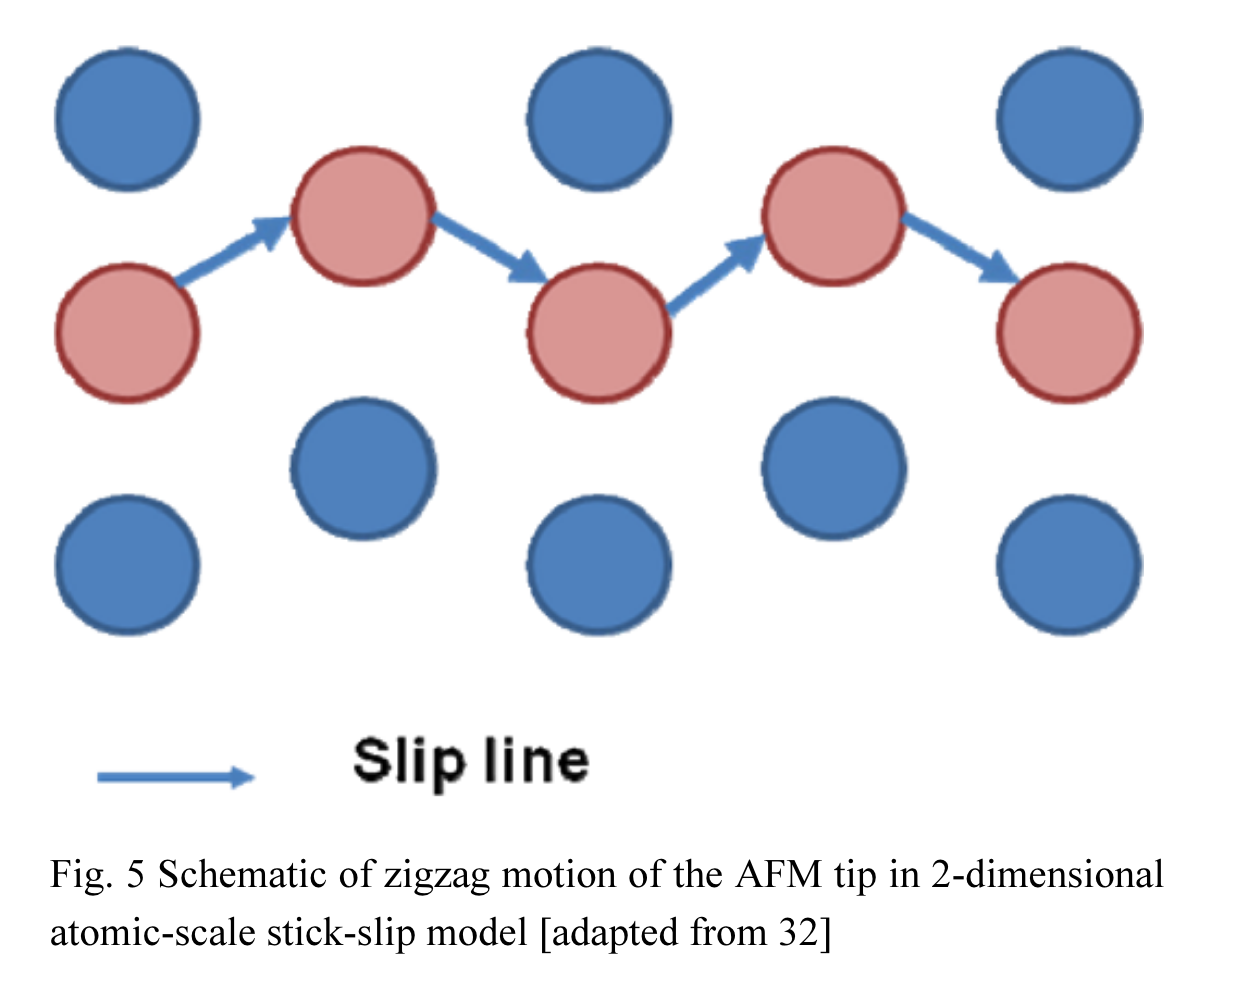
\includegraphics[width=0.5\linewidth]{figures/theory/slip_line.png}
%   \caption{\hl{Temporary} figure from~\cite{kim_nano-scale_2009}[p. 144]}
%   \label{fig:slip_line}
% \end{figure}


% the smallest force needed to set a slider in motion – is also dependent on the simulation time (a longer wait may lead to depinning when a short wait might not), and generally dependent on system size, often increasing with sub-linear scaling with the slider’s contact area. To address this kind of behavior in MD simulations, it is often necessary to resort to scaling arguments in order to extrapolate the large-area static friction from small-size MD simulations [131, 140]~\cite{Manini_2016}.


% Section 15.3. As shown in Section 15.1, the maximum value of the static friction and the slope of the turning points of the F(x) curves can be used to determine the corrugation U0 of the tip–surface interaction potential and the effective lat- eral stiffness k of the system. From Fig. 18.1(b) we estimate U0 ≈ 0.22 eV and k ≈1N/m.~\cite{gnecco_meyer_2015} p. 197






% Concerning stick-slip friction, another problem is that, unlike simulations, real experiments contain mesoscale or macroscale component intrinsically involved in the mechanical instabilities of which stick-slip consists. Here the comforting observation is that stick-slip is nearly independent of speed, so that so long as a simulation is long enough to realize a sufficient number of slip events, the results may already be good enough [148] ~\cite{Manini_2016}.


% A serious aspect of stick-slip friction which MD simulation is unable to attack is ageing. The slip is a fast event, well described by MD, but sticking is a long waiting time, during which the frictional contact settles very slowly. The longer the sticking time, the larger the static friction force necessary to cause the slip. Typicall experiments show a logarithmic increase of static friction with time [150]~\cite{Manini_2016}.

% Rate and state friction approaches, widely used in geophysics [151], describe phenomenologically frictional ageing, but a quantitative microscopic description is still lacking. Mechanisms invoked to account for contact ageing include chemical strengthening at the interface in nanoscale systems [152], and plastic creep phenomena in macroscopic systems [153].~\cite{Manini_2016}.


% See ``Selected Results of MD Simulations'' in~\cite{Manini_2016} p. 24.

% \section{Real life experimental procedures}
% From Introduction to Tribology, Second Edition, p. 526: \par The surface force
% apparatus (SFA), the scanning tunneling microscopes (STM), and atomic force and
% friction force microscopes (AFM and FFM) are widely used in nanotribological and
% nanomechanics studies.



% neg fric can be done, but can it be done with Kirigami
\section{Research questions}\label{sec:research_questions}
Based on the review of friction presented in~\cref{chap:friction}, it is evident that the behavior of friction is influenced by various factors, such as the specific system under investigation, the numerical modeling approach, and the physical conditions related to the environment and the probing of friction. In our study, we aim to investigate the frictional behavior
of a Kirigami sheet under the effects of strain. Previous studies have
demonstrated that strained Kirigami sheets are prone to out-of-plane buckling~\cite{PhysRevLett.121.255304, PhysRevResearch.2.042006} which is indicative of a possible transition between two distinct systems: An atomically flat interface and an asperity system. These systems are usually only studied
separately, and therefore, our primary objective is to investigate the possible frictional effects linked to strain-induced system transformations. In particular, we want to investigate the significance of the contact area and evaluate the hypothesis that reducing the contact area will lead to a decrease in friction. Additionally, we seek to examine the relationship between the friction-load curve and this phenomenon. For the sake of contributing new insight to the field of nanoscale
friction, we are interested in non-linear dependencies between
friction and stretching of various Kirigami designs. Drawing on this
perspective, we aim to investigate the prospects of achieving a negative friction coefficient for a system of coupled load and strain. In order to contextualize our findings within the theoretical framework, we will take into account the results from prior studies.


To gain a more comprehensive understanding of the potential applications of Kirigami design, we aim to develop a dataset based on \acrshort{MD} simulations that capture the frictional effects on Kirigami designs when subjected to strain and load. We intend to employ machine learning techniques to discern any meaningful trends in the data that may be used to inform future research endeavors. Specifically, we seek to leverage the machine learning model to facilitate an accelerated search for optimizing specific frictional properties. Our focus will be on evaluating the prospects of reducing or increasing the friction force, as well as reducing or increasing the friction coefficient for a coupled system of load and strain. Our main research questions can be summarized as follows.


\begin{enumerate}
  \item  How can we design an \acrshort{MD} simulation that provides a reliable foundation for an investigation of the frictional behavior for a Kirigami graphene sheet sliding on a substrate? How do physical conditions such as temperature and sliding speed control friction?
  \item How can we design an ensemble of Kirigami patterns for the investigation of its frictional properties with the scope of getting out-of-plane buckling and also randomized design features?   
  \item Can we control friction for a Kirigami sheet through Kirigami pattern design and straining of the sheet?
  \begin{enumerate}
    \item Does friction dependent on a changing contact area?
    \item How does the friction-load curve relate to strained Kirigami sheets?
    \item Are the effects of strain and pattern design significant when considered independently?
    \item Is the frictional behavior consistent with the Prandtl–Tomlinson, Frenkel-Kontorova and Frenkel-Kontorova-Tomlinson models? 
  \end{enumerate}
  \item Is it possible to utilize machine learning techniques to identify general trends in the relationship between friction and kirigami patterns, strain and load?
  \item Can we use a trained machine learning model to predict new designs through an accelerated search?
  \item What are the prospects of achieving a negative friction coefficient for a system of coupled load and strain through Kirigami design?
\end{enumerate}



% \begin{enumerate} % Try reducing the number of points here
%   \item Define a sheet indexing that allows for a unique mapping of patterns between a hexagonal graphene lattice representation to a matrix representation suited for numerical analysis. 
%   \item  Design a \acrshort{MD} simulation procedure to evaluate the frictional properties of a given graphene sheet under specified physical conditions such as load, stretch, temperature etc. 
%   \item Find and implement suitable kirigami patterns which exhibit out-of-plane buckling under tensile load. This includes the creation of a framework for creating variations within each pattern class. Additionally, create a procedure for generating different styles of random walk patterns.
%   \item Perform a pilot study of a representative subset of patterns in order to determine appropriate simulation parameters to use for further study along with an analysis of the frictional properties shown in the subset.
%   \item Create a dataset consisting of the chosen kirigami variations and random walk patterns and analyze data trends.
%   \item Train a neural network to map from the design space to physical properties such as mean friction, maximum friction, contact area etc.\ and evaluate the performance.
%   \item Perform an accelerated search optimizing for interesting frictional properties using the \acrshort{ML} model. This should be done both through the pattern generation procedures and by following a genetic algorithm approach. 
%   \item Use the most promising candidates from the accelerated search to investigate the prospects of creating a nanomachine setup that exhibits a negative friction coefficient. 
%   \item Study certain designs of interest with the scope of revealing underlying mechanisms. This includes simple correlation analysis but also a visualization of feature and gradient maps of the \acrshort{ML} network.
% \end{enumerate}






% What kind of friction effects can be associated to the stretching of Kirigami sheets.
% \item 


% How does the contact area relate to friction as the sheet buckles during stretching. 
% \item How does stretching effect friction.
% \item How does a non-stretched kirigami effect friction.
% \item what mechanism can we recognize from our expectations. 

% In general we will aim to design a friction simulation that gives stable result. We will consider the dependencies to temperautre, speed, spring constant as a means to comparing our results with the ...


% We are going to study the behvaiour of a kirigami sheet deforming under stretching which constitute a transition between system types. We will focus on how this transition effects the frictional behaviour and how this relates to parameters such as load and contact area. From the previous results we find the main expectations to our system which in \cref{tab:exp_summary}. By considering our system behaviour against these general expectations we can bring insight into some of the discrepancies related to different theoretical predictions and aim to pinpoint where our system belongs

% Experimental method lacks from not seeing the surface contact and retrieivng accurate data for what goes ons


% Size effects, edge effects and shape effects on commensurability is worth mentioning.  

%  By applying stretching to a Kirigami sheet we might
% transition the system from an atomically flat sheet towards an asperity system.
% If we were to follow asperity theory this should result in a reduced friction.
% If not, this might provide insight into the general importance of the contact
% area.

% In addition, the deformation of the sheet will most likely be connected to
% effect the commensurability which generally found to be of great importance.
% This could probably give rise to both an increase or a decrease in friction depending on whether we transition from an incommensurable to a commensurable state or vice versa. For a Kirigami modified system the dependence on load will bring insight to the discussion of how friction depends on load with two governing
% explanations being either true contact area or commensurability. 


% The dependencies for velocity, temperature and spring constant provide a reference point for the possible friction regimes, such as stick-slip versus smooth sliding or ballistic versus diffusive motion, which is essential for a more through comparison and understanding of our results. 



% Textwidth = 484,20988 pt*0,035146 pt/cm = 17,02 % \the\textwidth
% \begin{table}[H]
%   \begin{center}
%   \caption{Summary}
%   \label{tab:exp_summary}
%   \begin{tabular}{  M{5cm}  X{12cm} } \hline
%   \textbf{Stick slip} & Generally we expect to observe periodic stick-slip motion with a period matching the lattice constant(s) involved~\cite{mo_friction_2009}. This is however expected to be inhibited by high spring stiffness for the moving support, high temperature, system size and at large velocities. For the latter, we mainly refer to a ``smooth-looking'' force trace, which can still involve slips \hl{hmmm...} \\ \\
%   % At large velocities the reduced-models suggest a multiple slip behavior while experimental results suggest smooth sliding. This discrepancy might be explained by a different definition of smooth sliding as the multiple slip regime can produce seemingly ``smooth-looking'' force traces. Additionally, it is expected that the tendency of stick-slip behvaiour is reduced by increasing temperature and for incommensurability. \\ \\
%   \textbf{Static friction} & Static friction is expected to correlate with the presence of stick-slip motion. We expect it to be most pronounced for commensurable configurations with a possible disappearance for incommensurability. Moreover, static friction is expected to increase with system size, time in stationary contact and decreasing temperature. \\ \\
%   \textbf{Commensurability} & Both static and kinetic friction is expected to be highly sensitive to commensurability, through lattice spacing, the orientation of the flake relative to the substrate and the path of sliding along the substrate. By loading, rotating, cutting and stretching the sheet we might alter commensurability as well as a change of the spring constant can alter the translational freedom during sliding leading to a similar change in commensurability. \\ \\
%   \textbf{Friction evolution} \linebreak \textbf{(Friction strengthening)} & Friction evolution is found to be present in monolayer graphene resting on a substrate, and thus we expect this to be present in our simulation setup as well.  \\ \\
%   \textbf{Negative coef} & Previous result shows that a negative friction coefficient can be done, but these were related to a different system. However, alterations through stretching and corrugation have shown that it is possible to alter friction through deformations. By introducing a coupling between load and such deformations we might be able to achieve a negative coefficient.  \\ \\
%   \textbf{Normal load} & Generally an increasing friction force is expected with increasing load. Both non-dependent, sublinear and linear relationships can be expected. \\ \\
%   \textbf{Velocity} & Generally an increasing friction force is expected with increased sliding velocity. Numerical results suggest a viscous friction $F_k \propto v$ \\ \\
%   \textbf{Temperature} & From an experimental and model-based point of view friction is expected to decrease with temperature in a power law or exponential manner. However, for \acrshort{MD} simulations the transition from a diffusive to a ballistic regime at a velocity around 1--\SI{10}{m/s} is suggested to yield increasing friction with temperature.  \\ \\
%   \textbf{Contact area} & For the non-cut sheet we do not expect to see any noticeable change in contact area during loading. For a deforming sheet that successfully changes the contact area, it is theorized to alter the friction as well in a proportional manner.  \\
%   \hline
%   \end{tabular}
%   \end{center}
% \end{table}





% Formulate the research questions guiding the reading of the thesis moving on. 





 % Chapter 2
% \chapter{Molecular Dynamics}
% \cite[p. 18-]{Manini_2016}

Thanks to advances in computing algorithms and hardware the recent years has witnessed a remarkable increase in our ability to simulate tribological processes in realistic nano-frictional system \cite{Manini_2016}. A Molecular dynamics (MD) simulation can be considered as computational ``experiment''. Given a set of inital conditions and a mathematically model for interatomic forces we can solve Newton's (or equivalent) equation of motion by numerical integration [p. 303]{BHUSHAN20051507}. The interatomic forces are derived from interparticle interaction potentials, which is the heart of MD simulations and the specific choice of potentials can often be quite challenging.


Alternatives to the MD simulation like Ab inito methods calculate the interaction based on quantam mechanis (solving schrödinger) right?



% \begin{itemize}
%   \item MD simulation (classical or ab initio)
%   \item Basics of classical MD simulations: Integration and stuff
%   \item Ab initio simulation (quantum mechanics, solving schrödinger)
% \end{itemize}



% A promising compromise could possibly be provided by the so-called reactive potentials [120–122], capable of describing some chemical reactions, including interface wear with satisfactory computational efficiency in large-scale atomic simulations, compared to semi-empirical and first-principles approaches. \cite{Manini_2016}





% Quantum-mechanical calculations is more accurate but to numerical intensive.

% Despite recent progress in this respect, it is clear that there will always be
% interesting problems beyond the reach of ab initio approaches
% \cite{PhysRevB.37.6991}.





% The simplest approach to temperature control by adding the Langevin thermostat has been widely adopted, but more refinded methods has also been proposed and adopted (see \cite{Manini_2016} for more).

% Physically relevant quantities like the average friction force can be evaluated by carrying out averages over the model dynamics. The modeling most first of all adress equlibrium and near-equlibrium behvaiour where the fluctuation-dissipation theorem governs the conversion of mechanical energy into heat. But it most also deal with nonlinear dissipative phenomena such as instabilities and stick-slip.\cite{Manini_2016}

% Quantitative data can be obtained by analyzing the numerical output directly. [p. 303]{BHUSHAN20051507}


% Weak- nesses include a lack of quantum effects in classical atomistic dynamics, and perhaps more importantly, the fact that meaningless results can be obtained if the simulation conditions are incorrectly chosen. \cite[p. 303]{BHUSHAN20051507}


% Maybe read ``Computer Simulations 7 of Nanometer-Scale Indentation
% and Friction'' from \cite{BHUSHAN20051507}



\section{Potentials}
% \cite{PhysRevB.37.6991}



% Maybe include something like: The potentials is mainly chosen since they are used in somewhat similary studies, but we consider this an important point for further investigations. This includes a more thorough litterature review of the strength and weaknesses of each potential along with a test of how the friction properties change between different relevant potentials.


The potentials used in our MD simulation is mainly based on the of Li et al.\
\cite{li_evolving_2016} which have a somewhat similar MD friction simulation
setup. Li et al.\ impose a Silicon tip on the graphene sheet supported by a
Silicon substrate where we slide the whole sheet upon the substrate.
Nonetheless, this serves as a good anchor for the methodology of the setup. The
covalent bonds of C-C in graphene and Si-Si in the substrate is described by the
Tersoff and Stillinger–Weber potentials, respectively. A typical 12-6
Lennard–Jones potential is used to describe the van der Waals adhesive
interaction between graphene and the substrate. 

\subsection{General formulation of potentials (?)}
On a general note we can generalize the n-body potential as the expansion in
orders of participating atoms as 
\begin{align*}
  E = \sum_i V_1(\vec{r}_i) + 
      \sum_{\substack{i, j \\ i < j}} V_2(\vec{r}_i, \vec{r}_j) +  
      \sum_{\substack{i,j,k \\ i < j < k}} V_3(\vec{r}_i, \vec{r}_j, \vec{r}_i) + \cdots,
\end{align*} 
where $\vec{r}_n$ is the position of the $n$th particle and $V_m$ is called an
$m$-body potential  \cite{PhysRevB.37.6991}. The first one-body term corresponds
to an external potential, followed by the two-body term, the three-body term and
so on. The simplest model that includes particle interaction is the pair
potential truncating the expansion after the two-body term. A general feature of
the pair potentials is that they favor close-packed structures which is unsuited
to describe covalent bonds that take more open structures. In particular, pair
potentials are completely inapplicable to strongly covalent systems \cite{PhysRevB.37.6991}. In order to accomodate the description
of covalent bonds the natural step is thus to include the next step of the
expansion, the three-body terms, as we will see for the modeling of the C-C bonds in the graphene sheet and the Si-Si bonds in Silicon substrate. For the interaction between
the sheet and the substrate we use a Lennard Jones pair potential
describing the non-bonded van der Waals interaction. This simple interaction model between the moving object and substrate has come to be the standard in friction simulations \cite{zhu_study_2018}, \cite{ZHANG201585}, \cite{Yoon2015MolecularDS}, \cite{kim_nano-scale_2009}. 


\subsection{Lennard Jones}
\hl{TODO: Add potential curve figure} \\
% TODO: Add potential curve figure
This sections is based on \cite{docs_lammps_LJ}, \cite{C9CP05445F}, \cite{chem_libretexts_LJ}.

The Lennard-Jones (LJ) model is probably one of the most famous pair potentials
used in MD simulations. LJ models the potential energy between two non-bonding
atoms solely based on interatomc distance. The model accounts for attractive
forces arising from dipole-dipole, dipole-induced dipole and London
interactions, and repulsive forces that capture the hard core of overlapping wave functions at small distances (\hl{double check this statement}). Thus, it assummes
neutrally charged atoms and was orginally proposed for noble gases. The
classical 12-6 version of the model (refering to the power law of the repulsive
and attractive forces respectively) reads
\begin{align}
  E = 4\epsilon \left[\left(\frac{\sigma}{r}\right)^{12} - \left(\frac{\sigma}{r}\right)^6 \right ], \qquad r < r_c,
  \label{eq:LJ}
\end{align}
where $r$ is the interatomic distance with cut-off $r_c$, $\epsilon$ is the
depth of the potential well and $\sigma$ the interatomic distance where the potential is
zero. By solving for the potential minimum ($dE/dr = 0$) we find the equilibrium
distance to be $r_0 = \sigma 2^{1/6}$. This makes for a slightly more intuitive
interpration of $\sigma$ which effectively sets the equilirbium distance between
atoms, i.e.\ the dividing line for which the force is repulsive or
attractive. 


% While the LJ model in many ways is an oversimplified model that is
% insufficient in its description of ... (\hl{get source and concrete examples}) it is
% commonly used as a model for intermaterial interactions (between moving object
% and substrate) in friction studies.


\subsection{Stillinger weber}
% Todo: Add some potential curve figure? or figure of three body angles?
\hl{TODO: Add potential figure and or figure illustrating three body angles}.

This section is based on [\cite{docs_lammps_sw}, \cite{PhysRevB.31.5262}]

The stillinger weber potential takes the form of a three body potential
\begin{align*}
  E &=\sum_i \sum_{j>i} \phi_2(r_{i j})+\sum_i \sum_{j \neq i} \sum_{k>j} \phi_3(r_{ij}, r_{ik}, \theta_{ijk}),
\end{align*}
where $r_{ij}$ denotes the distance between atom $i$ and $j$ and $\theta_{ijk}$
the angle between bond $ij$ and $jk$. The summations is over all neighbours $j$
and $k$ of atom $i$ within a cut-off distance $r = a\sigma$. \\
The two-body term $\phi_2$ builds from the LJ model with the addition of an
exponetial cutoff term
\begin{align}
  \phi_2(r_{i j}) & =A_{ij} \epsilon_{ij}\left[B_{ij}\left(\frac{\sigma_{ij}}{r_{ij}}\right)^{p_{ij}} - \left(\frac{\sigma_{ij}}{r_{ij}}\right)^{q_{ij}}\right] \exp (\frac{\sigma_{ij}}{r_{ij}-a_{ij} \sigma_{ij}}).
  \label{eq:sw_2}
\end{align}

The model parameters $A$, $\epsilon$, $B$, $\sigma$, $p$, $q$ and $a$ comes with
$i,j$ indices to indicate that theese parameters should be specified for each
unique pair of atom types. However, in our case we will only provide a single
value for each model parameter as we are exclusively dealing with Si-Si bonds.
We see that the first term in \cref{eq:sw_2} is reminiscent of the LJ model
in \cref{eq:LJ} while the last term effectively drives the potential to
zero at $r=a\sigma$, which is thus the chosen cut-off distance for the potential
evaluation. With the model parameters for the Si-Si modelling (see \cref{tab:sw_param}) the cut-off becomes $\sim 3.8$ Å. \\
The three body term includes an angle dependency as
\begin{align}
  \phi_3(r_{ij}, r_{ik}, \theta_{ijk}) &= \lambda_{ijk} \ \epsilon_{ijk} \Big[\cos \theta_{ijk}-\cos \theta_{0,ijk}\Big]^2 \exp (\frac{\gamma_{ij} \sigma_{ij}}{r_{ij} - a_{ij} \sigma_{ij}}) \exp (\frac{\gamma_{ik} \sigma_{ik}}{r_{ik} - a_{ik} \sigma_{ik}}),
  \label{eq:sw_3}
\end{align}
where $\theta_{0,ijk}$ is the equilibrium angle. The first term of
\cref{eq:sw_3} includes an angle dependency analog to a harmonic oscillator
based on a cosine angle distance from the equilibrium angle. The final two terms
act again as a cut-off function by driving the potential to zero at $r_{ij} =
a_{ij}\sigma_{ij}$ and $r_{ik} = a_{ik}\sigma_{ik}$ respectively. \\ 
The parameters used for the Si-Si bond modeling is displayed in \cref{tab:sw_param} along with an interpretation of each model parameter.



\begin{table}[H]
  \begin{center}
  \caption{Parameters for the stilliner weber potential used for intermolecular interactions in the silicon substrate.}
  \label{tab:sw_param}
  \begin{tabular}{ | c | c | L{9cm} |} \hline
    Parameter & Value & Description \\ \hline 
    $\epsilon$ & 2.1683  & Individual depth of the potential well for each atom
    type pair/tiplets. \\ \hline
    $\sigma$ & 2.0951 & Distance for which the individual pair interactions has
    zero potential (analog to the LJ model). \\ \hline
    $a$ & 1.80 & The individual cut-off distance for each atom type pair. \\
    \hline
    $\lambda$ & 21.0 & The overall depth of the three-body potential well. \\
    \hline
    $\gamma$ & 1.20 & The shape of the three-body cut-off terms. \\ \hline
    $\cos{(\theta_0)}$ & -1/3 & Cosine of equilibrium angle. \\ \hline
    $A$ &  7.049556277 & The overall depth of the two-body potential well. \\
    \hline
    $B$ &  0.6022245584 & Scales the repulsion part of the two-body term. \\
    \hline
    $p$  & 4.0 & The power dependency for the repulsion part of the two-body
    term. \\ \hline
    $q$  & 0.0 & The power dependency for the attraction part of the two-body
    term. \\ \hline
    tol  & 0.0 & LAMMPS: Option to define a different cut-off than the
    theoretical of $r = a\sigma$. $tol = 0$ refers to the theoretical being
    used. \\ \hline
  \end{tabular}
  \end{center}
\end{table}



\subsection{Tersoff}
% Add figure similar to:
% https://en.wikipedia.org/wiki/Bond_order_potential#/media/File:Bond-order_interatomic_potential.png,
% showing bond order curves.


% https://interatomic-potentials.readthedocs.io/en/latest/doc/tersoff.html
% https://chem.libretexts.org/Bookshelves/
% Physical_and_Theoretical_Chemistry_Textbook_Maps/Supplemental_Modules_(Physical_and_Theoretical_Chemistry)/Chemical_Bonding/Fundamentals_of_Chemical_Bonding/Bond_Order_and_Lengths
This section is based on [\cite{docs_lammps_tersoff}, \cite{PhysRevB.37.6991}].


The tersoff potential abandon the idea of a general $n$-body form and attempts
instead to build the model on a more physics informed approach; The more
neighbours an atom has the weaker the bonds will be. Thus it introduces the bond
order (bond strentgh), that is environment specific and decrease with increasing
bond coordination (number of neighbours for a given atom). The potential energy
is taken to have the form

\begin{align*}
  E &= \sum_i E_i = \frac{1}{2}\sum_{i \ne j} V_{ij}, \\
  V_{ij} &= f_C(r_{ij}) \big[f_R(r_{ij}) + b_{ij}f_A(r_{ij})  \big],
\end{align*}

% where the total potential energy is decomposed into an atom site energy $E_i$
% and a bond energy $v_{ij}$. 
where the total potential energy is decomposed into a bond energy $V_{ij}$. The
indices $i$ and $j$ run over the atoms of the system with $r_{ij}$ denoting the
distance between atom $i$ and $j$. Notice that the sum includes all combinations
of $i,j$ where $i\ne j$ meaning that the same bond is double counted which is
the reason for the additional factor $1/2$. The reasoning behind comes from the
asymmetry of the bond order $b_{ij}\ne b_{ji}$ leading to a $V_{ij}\ne V_{ji}$.
The bond energy is composed of a repulsive term $f_R$, arising from overlapping
wave functions, and an attractive term $f_A$ associated with bonding. $f_c$ is
simply a smooth cut-off function to increase computational efficiency. $b_{ij}$
represent the bond order, i.e. the strength of the bonds, which depends
inversely on the number of bonds, the bond angles ($\theta_{ijk}$) and
optionally the relative bonds lengths ($r_{ij}$, $r{jk}$). Notice that an
additional cut-off term $a_{ij}$ was orginally multiplied to $f_R$ as a way of
including terms that limit the range of the interactions to the first neighbour
shell. These kind of limitations is already included in $b_{ij}$ for the
attractive term $f_A$ but is often omitted for the repulsive term $f_R$, and we
do so to by setting $a_{ij} = 1$. \\
The cut-off function $f_C$ goes from 1 to 0 over a small interval range $R \pm
D$ as
\begin{align*}
  f_C(r) =
  \begin{cases}
    1 & r < R - D \\
    \frac{1}{2} - \frac{1}{2} \sin{(\frac{\pi}{2} \frac{r - R}{D})} & R - D < r < R + D\\
    0 & r > R + D
  \end{cases},
\end{align*}
which is continuous and differentiable for all $r$. $R$ is usually chosen to
include only the first neighbour shell. \\
The repulsive and attractive terms $f_R$ and $f_A$ is modelled as an exponetial
function, similar to a morse potential, 
\begin{align*}
 f_R(r) &= A \exp(-\lambda_1 r), \\
 f_A(r) &= -B \exp \big(-\lambda_2 r\big).
\end{align*}

The novel feature of the model lies in modeling of the bond order $b_{ij}$ which
includes three-body interactions by summing over a third atom $k \ne i,j$ within
the cut-off $r_{ik} < R + D$ as shown in the following.

\begin{align}
  b_{i j} & =\big(1+\beta^n \zeta_{i j}^n\big)^{-\frac{1}{2 n}} \\
  \zeta_{i j} & =\sum_{k \ne i,j} f_C(r_{i k}) g\Big(\theta_{i j k}\left(r_{i j}, r_{i k}\right)\Big) \exp \left(\lambda_3{ }^m\big(r_{i j}-r_{i k}\right)^m\big) \\
  g(\theta) & =\gamma_{i j k}\left(1+\frac{c^2}{d^2}-\frac{c^2}{\left[d^2+\left(\cos \theta-\cos \theta_0\right)^2\right]}\right).
  \label{eq:tersoff_bond_order}
\end{align}

In \cref{eq:tersoff_bond_order} $\zeta_{i,j}$ is an effective coordination
and $g(\theta)$ captures angle dependency as it is minimized at the equilibrium
angle $\theta = \theta_0$. \\
The parameters used to model the graphene C-C bonds is summarized in \cref{tab:tersoff_param}



\begin{table}[H]
  \begin{center}
  \caption{Parameters for the tersoff potential used for intermolecular interations in the graphene sheet}
  \label{tab:tersoff_param}
  \begin{tabular}{ | c | c | L{9cm} |} \hline
    Parameter & Value & Description \\ \hline 
    $m$ & 3.0 & Default (not used since $\lambda_3 = 0$ ) \\ \hline
    $\gamma$ & 1.0 & ... \\ \hline
    $\lambda_3$ & 0.0 Å$^{-1}$ & ... \\ \hline
    $c$ & \num{3.8049e4} & Strength of the angular effect \\ \hline
    $d$ & 4.3484 & Determines the ``sharpness'' of the angular dependency \\
    \hline
    $\cos{(\theta_0)}$ & -0.57058 & Cosine of the equilibrium angle \\ \hline
    $n$ & 0.72751 & Power law exponent for the bond order dependency \\ \hline
    $\beta$ & \num{1.5724e-7} & ... \\ \hline
    $\lambda_2$ & 2.2119 Å$^{-1}$ & Decay of repulsion potential term \\ \hline
    $B$ & 346.74 eV & Attractive potential term minimum at core ($ r_{ij} = 0$).
    \\ \hline
    $R$ & 1.95 Å & Center distance for cut-off \\ \hline
    $D$  & 0.15 Å & Thickness of cut-off layers \\ \hline
    $\lambda_1$ & 3.4879 Å$^{-1}$ & Decay of repulsion potential term \\ \hline
    $A$ & 1393.6 eV & Repulsion potential term at core ($ r_{ij} = 0$) \\ \hline
  \end{tabular}
  \end{center}
\end{table}



\section{Integration}
% https://www.eng.uc.edu/~beaucag/Classes/AdvancedMaterialsThermodynamics/Books/%5BComputational%20science%20(San%20Diego,%20Calif.)%5D%20Daan%20Frenkel_%20Berend%20Smit%20-%20Understanding%20molecular%20simulation%20_%20from%20algorithms%20to%20applications%20(2002,%20Academic%20Press%20)%20-%20libgen.lc.pdf

Having defined a system of particles governed by interartomic potentials we need
to move the system forward in time. By solving Newtons equations of motion we
effectively sample the microcanonical ensemble characterized by a
constant number of particles $N$, volume $V$ and energy $E$, hence denoted NVE.
Newtons equaitons of motion read
\begin{align}
  m_i \frac{d^2 \vec{r}_i}{dt^2} = \vec{F}_i = -\nabla U_i
  \label{eq:NE}
\end{align}
where $i$ is the particle index and $m_i$ its mass, $\vec{r}_i = (x_i, y_i,
z_i)$ the position, $t$ is time,  $\nabla_i = (\frac{\partial}{\partial x_i},
\frac{\partial}{\partial y_i}, \frac{\partial}{\partial z_i})$ and $U_i$ the
potential energy. The potential energy is a function of the particle
positions of nearby particles depending on the specefic potential in use. Since
the forces defined by the potentials is conservative we expect the energy of the
solution to be conserved. We can redefine \cref{eq:NE} in terms of two coupled
first order differential equations 
\begin{align}
  \dot{\vec{v}}_i(t) = \frac{\vec{F}}{m_i}, \qquad \dot{\vec{r}}_i(t) = \vec{v}_i(t),
  \label{eq:NE_2}
\end{align}
where $\dot{x} = dx/dt$ (Newton's notation) and $\vec{v} = (v_x, v_y, v_z)$ is
velocity. Numerically we can solve the coupled equations by
integrating over discrete timnesteps. That is, we discretize the solution into
temporal steps $t_k = t_0 + k\Delta t$ with start time $t_0$ and time-step $\Delta t$. 

% However small erros applied by the discrete integraiton algorithm we end up
% having an energy error. This is sensitive to time step. 


\subsection{Velocity Verlet}
% http://www.physics.drexel.edu/~valliere/PHYS305/Diff_Eq_Integrators/Verlet_Methods/Diffrntleqn3.pdf
% ttps://www2.ph.ed.ac.uk/~dmarendu/MVP/MVP03.pdf

A common algorithm to integrate Newtons equation of motion (as formulated in
\cref{eq:NE_2}) is the \textit{velocity verlet}. We can derive the algorithm
by the use of Taylor expansions. We begin by expanding the next-step position
vector $\vec{r}_i(t + \Delta t)$ at time $t$
\begin{align}
  \vec{r}_i(t + \Delta t) &= \vec{r}_i(t) + \dot{\vec{r}}_i(t) \Delta t + \frac{\ddot{\vec{r}}_i(t)}{2} \Delta t^2 + \mathcal{O}(\Delta t^3) \label{eq:vv_comp1},
\end{align}
where $\ddot{\vec{r}} = d^2\vec{r}/dt^2$ and $\Delta t^n$ is simply the relaxed
notation for $(\Delta t)^n$. Similar we take the expansions of the next-step
velocity vector $\vec{v}_i(t+\Delta t)$ at time $t$ 
\begin{align}
  \vec{v}_i(t+\Delta t) = \vec{v}_i(t) + \dot{\vec{v}}_i(t) \Delta t + \frac{\ddot{\vec{v}}_i(t)}{2}\Delta t^2 + \mathcal{O}(\Delta t^3).
  \label{eq:tay_v1}
\end{align}
Finnally, by taking the expansion of $\dot{\vec{v}}_i(t+\Delta t)$ we can
eliminate the $\ddot{\vec{v}}_i$-term in \cref{eq:tay_v1} and simplify it
as shown in the following.
\begin{align}
  \dot{\vec{v}}_i(t+\Delta t) &= \dot{\vec{v}}_i(t) + \ddot{\vec{v}}_i(t) \Delta t + \mathcal{O}(\Delta t^2) \nonumber \\
  \frac{\ddot{\vec{v}}_i(t)}{2}\Delta t^2 &= \frac{\Delta t}{2}\Big( \dot{\vec{v}}(t+\Delta t) - \dot{\vec{v}}_i(t)\Big) + \mathcal{O}(\Delta t^3) \nonumber \\
  &\Downarrow \nonumber \\
  \vec{v}_i(t+\Delta t) &= \vec{v}_i(t) + \dot{\vec{v}}_i(t) \Delta t + \frac{\Delta t}{2}\Big( \dot{\vec{v}}_i(t+\Delta t) - \dot{\vec{v}}_i(t)\Big) + \mathcal{O}(\Delta t^3) \nonumber \\
  &=  \vec{v}_i(t) + \frac{\Delta t}{2}\Big( \dot{\vec{v}}_i(t) +  \dot{\vec{v}}_i(t+\Delta t)\Big) + \mathcal{O}(\Delta t^3).
  \label{eq:vv_comp2}
\end{align}
By combining \cref{eq:vv_comp1} and \cref{eq:vv_comp2} and using
Newton's second equation $\dot{\vec{v}} = \vec{F}_i(t)/m_i = $ and $\vec{v} =
\dot{\vec{r}}$ we arrive at the final scheme
\begin{align*}
  \vec{r}_i(t + \Delta t) &= \vec{r}_i(t) + \vec{v}_i(t) \Delta t + \frac{\vec{F}_i(t)}{2m_i}\Delta t^2 + \mathcal{O}(\Delta t^3), \\
  \vec{v}_i(t+\Delta t)  &= \vec{v}_i(t) + \frac{\vec{F}_i(t) + \vec{F}_i(t+\Delta t)}{2m_i}  \Delta t + \mathcal{O}(\Delta t^3).
\end{align*}
The scheme will give a local error of order $\Delta t^3$ corresponding to a
global error of $\Delta t^2$. One of the most popular ways to implement this
numerically is as stated in the following steps.
\begin{enumerate}
  \centering
  \item Calculate $v_{k+\frac{1}{2}} = v_k + \frac{F_k}{2m} \Delta t$.
  \item Calculate $r_{k+1} = r_k + v_{k+\frac{1}{2}} \Delta t$.
  \item Evaluate the force $F_{k+1} = F(r_{k+1})$.
  \item Calculate $v_{k+1} = v_{k+\frac{1}{2}} + \frac{F_{k+1}}{2m} \Delta t$  
\end{enumerate}





% \begin{align*} \vec{r}_i(t + \Delta t) &= \vec{r}_i(t) + \vec{v}_i(t) \Delta t
%   + \frac{\vec{F}_i(t)}{2m_i}\Delta t^2 + \mathcal{O}(\Delta t^3), \\
%   \vec{v}_i(t+\Delta t)  &= \vec{v}_i(t) + \frac{\vec{F}_i(t) +
% \vec{F}_i(t+\Delta t)}{2m_i}  \Delta t + \mathcal{O}(\Delta t^3). \end{align*}
% This scheme will give a local error of order $\Delta t^3$ corresponding to a
% global error of $\Delta t^2$. 

% Lets descritize the time as $t_k = k * \Delta t$ with position $\vec{r}_k$ and
% velocity $\vec{v}_k$. At time $t_k$ the acceleration is given $\vec{a}_k =
% F(\vec{r}_k)/m$. We get the implementation steps as follows \begin{enumerate}
% \item Calculate $\vec{r}_{k+1} = \vec{r}_k + \vec{v}_k \Delta t +
% \frac{F(\vec{r}_k)}{2m}(\Delta t)^2$ \item Evaluate $F(\vec{r}_{k+1})$ \item
% Calculate $\vec{v}_{k+1} = \vec{v}_k + \frac{F(\vec{r}_k) +
% F(\vec{r}_{k+1})}{2m} \Delta t$ \end{enumerate}


% It is sometimes expressed as the following. This is mathematically the same,
% but is it computaitonally more efficient?


% \begin{align*} \mathbf{r}_i(t+\delta t) & =\mathbf{r}_i(t)+\mathbf{v}_i(t)
%   \delta t+\frac{\mathbf{f}_i(t)}{2 m_i} \delta t^2 \\
%   \mathbf{v}_i(t+\delta t / 2) & =\mathbf{v}_i(t)+\frac{\delta t}{2}
%   \frac{\mathbf{f}_i(t)}{m_i} \\
%   \mathbf{f}_i(t+\delta t) & =\mathbf{f}_i\left(\mathbf{r}_i(t+\delta
%   t)\right) \\
%   \mathbf{v}_i(t+\delta t) & =\mathbf{v}_i(t+\delta t / 2)+\frac{\delta t}{2}
%   \frac{\mathbf{f}_i(t+\delta t)}{m_i} \end{align*}

%   % https://www2.ph.ed.ac.uk/~dmarendu/MVP/MVP03.pdf Further they suggest this
%   to be the most used algorithm

%   \begin{align*} \mathbf{v}_i(t+\delta t / 2) & =\mathbf{v}_i(t)+\frac{\delta
%     t}{2} \frac{\mathbf{f}_i(t)}{m_i} \\
%     \mathbf{r}_i(t+\delta t) & =\mathbf{r}_i(t)+\mathbf{v}_i(t+\delta t / 2)
%     \delta t \\
%     \vec{f}_i(t + \delta t) &= \vec{f}_i(\vec{r}_i(t+ \delta t)) \\
%     \mathbf{v}_i(t+\delta t) & =\mathbf{v}_i(t+\delta t / 2)+\frac{\delta
%   t}{2} \frac{\mathbf{f}_i(t+\delta t)}{m_i} \end{align*} Make sure to check
%   this out. 

\section{Thermostats}

As we already mentioned above in Sec. 2, any kind of sliding friction involves mechanical work, some of which is then transformed into heat (the rest going into structural transformations, wear, etc.). The heat is then transported away by phonons (and electrons in the case of metallic sliders) and eventually dissipated to the environment \cite{Manini_2016}.



Likewise all excitations generated in the simulations should be allowed to propagate in the system and disperese in the bulk of both sheet and substrate. Due to small simulation size theese is likely to relfect back and ´´pile up'' unphysically Thus in order to avoid continuous heating and attain a steady state the (Joule) heat must be removed at a steady state. This is very the viscous damping of the langevin equations enter the picture. It can be difficulut to set the value $\gamma$ for the magnitude of this damping. The unphysical introduction of heat sink can be mittigated by some modifictions he mention, which is kind of next level I guess. 


\subsection{Langevin thermostat} \label{sec:langevin}

% Check out \cite{Manini_2016} for a good theory section on this that I had
% completely missed when writing this!

% Based on
% https://www.uio.no/studier/emner/matnat/fys/FYS4130/v19/pensumliste/stat-phys_2019.pdf

% http://physics.gu.se/~frtbm/joomla/media/mydocs/LennartSjogren/kap6.pdf


In order to control the temperature of the system we introduce the so-called
Langevin thermostat. This is a stochastic thermostat that modifies Newtons
equation of motion such that solution lies in the canonical ensemble
characterized by a constant number of particles $N$, constant volume $V$ and
constant temperature $T$, hence denoted NVT. The canonical ensemble system is
represented by the finite system being in contact with an infinte heat bath of
temperature $T$. The NVT ensemble is equivalent to sampling a system in
theromodynamic equilibrium where the weight of each microscopic state is given
by the boltzmann factor $\exp[-E/(k_B T)]$.

The Langevin equation is the modified version of Newtons second law for a
Brownian particle. A brownian particle is a small particle suspendend in liquid,
e.g. pollen or dust, named after Robert brown (1773–1858) who was the first to
observe its jittery motion. The Langevin equation describes this motion as the
combination of viscous drag force $ -\gamma \vec{v}$, where $\gamma$ is a
positive friction coefficient and $\vec{v}$ the velocity vector, and a random
fluctuation force $\vec{R}$. The langevin equation reads
\begin{align}
  m \frac{d \vec{v}}{dt} = -\gamma \vec{v} + \vec{R}
  \label{eq:Langevin}
\end{align}
where $m$ is the particle mass. This effectively describes the particle of
interest, the brownian particle, as being suspendend in a sea of smaller
particles. The collision with these smaller particles is modelled by the drag
force and the fluctuation force. We notice that if the fluctuation force is
excluded \cref{eq:Langevin} becomes 
\begin{align*}
  m \frac{d \vec{v}}{dt} = -\gamma \vec{v} \quad \Rightarrow \quad 
  \vec{v}_i(t) = v(0)e^{- \frac{\gamma t}{m}},
\end{align*}
where the solution shows that the brownian particle will come to a complete stop
after a long time ${\vec{v}_i(t\to\infty) \to \vec{0}}$. This is in violation
with the equipartion theorem
\begin{align*}
  \frac{1}{2}m\langle v^2 \rangle_{eq} = \frac{k_B T}{2},
\end{align*}
and hence the fluctuation force is nessecary to obtain the correct equilibrium. 

The following calculations are done in one dimension in order to simplify the
notation. We describe the statistical nature of the collisions as a sum of
independent momentum transfers
\begin{align*}
  \Delta P = \sum_i^N \delta p_i
\end{align*}

where $\Delta P$ denotes the change of momentum after $N$ momentum transfers
$\delta p_i$ from the environment to the brownian particle. We assume the first
and second moments $\langle \delta p \rangle = 0$ and  $\langle \delta p \rangle
= \sigma^2$. When $N$ is large the central limit theorem states that the random
variable $\Delta P$ has a gaussian distribution with  $\langle P \rangle = 0$
and $\langle \Delta P^2 \rangle = N\sigma^2$. If we consider the momentum change
$\Delta P$  over a discrete time $\Delta t$, where the number of collisiosn is
proportional to time $N \propto \Delta t$, the corresponding fluctuation force
$R = \Delta P / \Delta t$ will have a variance 


\begin{align*}
  \langle R^2 \rangle = \frac{\langle \Delta P^2 \rangle}{\Delta t^2} = \frac{N \sigma^2}{\Delta t^2}  \propto \frac{1}{\Delta t}.
\end{align*}

In a computer simulation we need to pick a random force $R(t)$ from a Gaussian
distribution every time-step $\Delta t$. These forces will not be correlated as
long as $\Delta t$ is larger than the correlation time of the forces from the
molecules which we will assume for this model (I think there exist corrections
for this to refer to here). With this assumption we can write the correlation
function as 
\begin{align}
  \langle R(t) R(0) \rangle = 
  \begin{cases}
    \frac{a}{\Delta t}, & |\Delta t| < \Delta t/2 \\
    0, & |\Delta t| > \Delta t/2,
    \label{eq:disc_corr}
  \end{cases}
\end{align}

where $a$ is some strength of (...?). In the limit $\Delta t \to 0$ the
correlation function becomes

\begin{align}
  \langle R(t)R(0) \rangle = a \delta(t),
  \label{eq:F_corr}
\end{align}

% Note that the delta function is justified by the fact that the characteristic frequencies of the phonon and electron excitations are much shorter than the hopping rate of the tip between the minima of the interaction potential \cite{gnecco_meyer_2015}

where $\delta$ denotes the dirac delta function. This is valid for all spatial
coordinates which will all be independent of each other. Since both the drag
force and the fluctuation force originate from the molecular fluid, where the
drag force $-\alpha \vec{v}$ is velocity dependent it is reasonible to assume
that fluctuation force is independent of velocity, i.e. $\langle R_i v_j \rangle
= 0$ for all cartesian indices $i$ and $j$.


% Since $\langle \tilde{F} \rangle = 0$ the random force (fluctuating force)
% will not conribute with a average decay (change) to the velocity. The
% macroscopic decay comes from the friction force (dissipitative force)  $-ma
% =\alpha v$ (give variable explanation). 

In the following we will attempt justify the Langevin equaiton (why it is like
it is) and determine the relationship between the drag coefficient $\gamma$ and
the random force $R$.


From the Langevin equation \cref{eq:Langevin} we can compute the velocity
autocorrelation function (Move to appendix?). We do this in one dimension for
simplicity. We begin by multiplying by $(e^{\gamma t /m})/m$

\begin{align*}
  \dot{ v}(t)e^{\gamma t /m} + \frac{\gamma}{m} v(t)e^{\frac{\gamma t}{m}}  = \frac{ F}{m}e^{\frac{\gamma t}{m}},
\end{align*}
and integrate from $t = -\infty$. By the use of integration by parts on the
latter term on the left hand side we calculate the velocity 
\begin{align*}
  \int_{-\infty}^t dt' \ \dot{ v}(t')e^{\frac{\gamma t'}{m}} + \frac{\gamma}{m} v(t)e^{\frac{\gamma t'}{m}} &=  \int_{-\infty}^t dt' \ e^{\frac{\gamma t'}{m}} \frac{ F(t')}{m}  \\
  \int_{-\infty}^t dt' \ \dot{ v}(t')e^{\frac{\gamma t'}{m}} + \left(\Big[ v(t')e^{\frac{\gamma t'}{m}}\Big]_{-\infty}^t - \int_{-\infty}^t dt' \ \dot{ v}(t')e^{\frac{\gamma t'}{m}}\right) &= \int_{-\infty}^t dt' \ e^{\frac{\gamma t'}{m}} \frac{ F(t')}{m}  \\
   v(t) &= \int_{-\infty}^t dt' \ e^{\frac{-\gamma(t - t')}{m}} \frac{ F(t')}{m},
\end{align*}
where $e^{\frac{-\gamma t}{m}}$ plays the role of a response function. We can
then calculate the autocorrelation 
\begin{align*}
  \big\langle  v(t) v(0) \big\rangle &= \int_{-\infty}^t dt_1 \ \int_{-\infty}^0 dt_2 \ e^{\frac{t - t_1 - t_2}{m}} \frac{\langle  F(t_1)  F(t_2) \rangle}{m^2} \\
  &= \int_{-\infty}^t dt_1 \ \int_{-\infty}^0 dt_2 \ e^{\frac{t - t_1 - t_2}{m}} \frac{a \delta(t_1 - t_2)}{m^2} \\
  &= \int_{-\infty}^0 dt_2 \ e^{\frac{t - 2t_2}{m}} \frac{a}{m^2} = \frac{a}{2m\gamma}e^{-\frac{\gamma t}{m}},
\end{align*}
where we used \cref{eq:F_corr} and the fact that the integration commutes
with the average (we are allowed to flip the order). By comparing this with the
equipartition theorem we get 
\begin{align*}
  \frac{1}{2}m\langle  v^2 \rangle &= \frac{k_BT}{2} \\
  \frac{1}{2}m\langle  v(0) v(0) \rangle = \frac{a}{4\gamma} &= \frac{k_BT}{2} \\
  a &=  2\gamma k_B T \\
\end{align*}
We notice the appereance of $\gamma$ meaning that the magnitude of the
fluctuations increase both with friction and temperature. Further we can
integrate the velocity over time to get displacement $x(t)$ and show that the
variance (show this? In appendix maybe?) is 
\begin{align*}
  \big\langle x^2(t) \big\rangle = \frac{2 k_B T}{\gamma} \left(t - \frac{m}{\gamma}\left(1 - e^{-\gamma t/m} \right) \right),
\end{align*}
where for $t \gg m/\gamma$ only the $t$-term survies yielding
\begin{align*}
  \langle x^2(t) \rangle = 2 k_BTt/\gamma.
\end{align*}
In 1D, the diffusion constant $D$ is related to the variance as $\langle x^2
\rangle = 2Dt$, meaning that this represents the einstein relation $D = \mu k_B
T$ with the mobility $\mu = 1/\gamma$.

when $t \ll m/\gamma$ we use the Taylor expansion $1 - e^{-x} \approx x - x^2/2$
for $x\ll 1$ to get 
\begin{align*}
  \big\langle x^2(t) \big\rangle = \frac{k_B T}{m} t^2
\end{align*}
which exactly mathces the thermal velocity
\begin{align*}
  v_{\text{th}} \frac{\big\langle x^2(t) \big\rangle}{t^2} = \frac{k_B T}{m}
\end{align*}
which follows from the equipartition theorem. The finite correlation time
$\gamma/m$ hence describe the crossover from the ballistic regime $\sqrt{\langle
x^2(t) \rangle} \propto t$ to the diffusive regime $\sqrt{\langle x^2(t)
\rangle} \propto \sqrt{t}$.

Introduce the fluctuation-dissipation theorem concept earlier since this is a
motivaiton for the Langeivn equation. 


% Of course, this approach is not rigorous, since the relevant particles
% colliding with each given simulated atom are already all included in the
% conservative and deterministic forces explicitly accounted for by the “force
% field”. The Langevin approach is quite accurate to describe small
% perturbations away from equilibrium, but it may fail quite badly in the
% strongly out-of-equilibrium nonlinear phenomena which are the target of the
% present paper.  \cite{Manini_2016}

\subsection{Implementing Langevin}
% https://docs.lammps.org/fix_langevin.html

% https://www2.ph.ed.ac.uk/~dmarendu/MVP/MVP03.pdf

% https://chem.libretexts.org/Bookshelves/Physical_and_Theoretical_Chemistry_Textbook_Maps/Non-Equilibrium_Statistical_Mechanics_(Cao)/01%3A_Stochastic_Processes_and_Brownian_Motion/1.04%3A_The_Langevin_Equation

% \cite{Hunenberger2005}(pp. 115, 120-121) \cite{docs_lammps_langevin}

% Make a note: We only introduce the thermostat to the edges of the parts of
% interest as the thermostat might disrupt important properties of the
% simulation (accoridng to Henrik, get a source/example on this).


The implementation of the Langevin equation into LAMMPS follows
\cite{PhysRevB.17.1302} and updates the force vector for each particle as 

\begin{align}
  \vec{F} &= \vec{F_c} + \vec{F}_{f} + \vec{F}_{r} \nonumber \\
  &= -\nabla U - \gamma m \vec{v} + \sqrt{\frac{2 k_B T m \gamma}{\Delta t}}\vec{h}(t)
  \label{eq:Langevin_generalized}
\end{align}
where $\vec{F_c}$ is the conservative force computed via the usual
inter-particle interactions described by the potential $U$, $\vec{F}_f$ is the
drag force and $\vec{F}_r$ is the random fluctuation force where $\vec{h}$ is a
random vector drawn from a normal distribution with zero mean and unit variance.
Notice that this generalized description of the Langevin equation deviates from
the presentation in \cref{eq:Langevin} since we have added the conservative
force $\vec{F_c}$, but also by the appearance of the mass in both the drag force
and the fluctuation force due to the introduction of damping. It is beyond out
scope to comprehend this. However, the fact that $\Delta t$ now appears in the
denomiator for the random force variance $2k_B T m \gamma / \Delta t$ is due to
the fact that we have discretized time. This in agreement with the formulation
in \cref{eq:disc_corr}. By applying \cref{eq:Langevin_generalized} we
get the refined velocity verlet scheme


\begin{align*}
  \vec{v}_i(t + \Delta t/2)  &= \vec{v}_i(t) - \frac{\Delta t}{2}\left(\frac{\nabla_i U(t)}{m_i} + \gamma \vec{v}_i \right) + \sqrt{\frac{k_B T \gamma \Delta t}{2m_i}} \vec{h}_i \\ 
  \vec{r}_i(t + \Delta t) &= \vec{r}_i(t) + \vec{v}_i(t + \Delta t/2) \Delta t \\
  \vec{v}_i(t + \Delta t) &= \vec{v}_i(t+ \Delta t/2) - \frac{\Delta t}{2}\left(\frac{\nabla_i U(t + \Delta t)}{m_i} + \gamma \vec{v}_i(t + \Delta t/2) \right) + \sqrt{\frac{k_B T \gamma \Delta t}{2m_i}} \vec{h}_i
\end{align*}
% A little unsure whether the factor 2 in the denominator in the random force is
% correct.
with new random vector $\vec{h}_i$ for each particle and each update. Notice
however, that LAMMPS only apply this scheme to the particle groups with the
thermostat on. 

% \newpage

% \begin{align} \vec{F}_i &= \vec{f}_{i} + \vec{f}_{f,i} + \vec{f}_{r,i}
%   \nonumber \\
%   m_i \ddot{\vec{r}}_i &= \vec{f}_{i} - \gamma_i \vec{p}_i + \vec{R}_i(t)
%   \label{eq:langevin_old} \end{align}

% where $m_i$ is the mass of particle $i$ $\vec{r}_i$ the position vector. The
% random force $\vec{R}_i(t)$ is described as gaussian white noise and have the
% following properties. 

% \begin{enumerate} \item It is uncorrelated with the velocities
%   $\dot{\vec{r}}(t)$ and deterministic forces $\vec{f}_i(t')$ at previous
%   times $t' < t$. \item The time average is zero: $\langle \vec{R}(t) \rangle
%   = \vec{0}$. \item The mean-square components evaluate to $2m_i\gamma_i k_B
%   T$. \item The force component of particle $i$ $R_{i,\mu}$ along cartesian
%   axis $\mu$ is uncorrelated with any component of particle $j$ $R_{i,\nu}$
%   along cartesian axis $\nu$, unless $i=j$, $\mu=\nu$ and $t=t'$.
%   \end{enumerate}

% The ladder two conditions can be formulated as

% \begin{align*} \langle R_{i,\mu}(t) R_{j,\nu}(t') \rangle = 2m_i \gamma_i k_B
%   T  \delta_{ij} \delta_{\mu\nu}\delta(t'-t),  
% \end{align*}

% where $\delta_{\cdot\cdot}$ is the Kronecker Delta function and
% $\delta(\cdot)$ is the Dirac Delta function. It can be shown that a trajectory
% generated by integrating the Langevin equations of motion
% (\cref{eq:langevin_old}) maps a cononical distribution of microstates at
% temperature $T$. \cite{Hunenberger2005}(p.121). (Can I say something more
% about the relationship between the friction froce and the random force - How
% to the balance to give NVT. Is the proof complicated?)\\

% In practice the implementation of the thermostat is implemented discretely by
% updating the force on each particle by the addition of the described forces
% $f_f$ and $f_r$ for each particle. In LAMMPS this is controlled by the user
% defined damping factor ``damp'' = $\gamma^{-1}$ in units of time whih control
% how fast we are going to reach the temperature equlibrium. Thus the
% documentation (\cite{docs_lammps_langevin}) defines the added forces as

% \begin{align*} f_f &= -\frac{m}{\text{damp}}, \qquad f_r \propto \sqrt{\frac{m
%   k_B T}{dt \ \text{damp}}} \end{align*}

% where $v = \dot[r]$ is the velocity. The definition of $f_f$ falls straight
% out of the definition above in \cref{eq:Langevin} while the
% proportionality of $f_r$ comes from

% \begin{align*} \sqrt{\langle R(t)^2 \rangle} = \sqrt{2m\gamma k_B T} \propto
%   \sqrt{\frac{m k_B T}{\text{damp}}} \end{align*}

% Thus we have $f_r \propto \sqrt{\langle R(t)^2 \rangle / dt}$ which I do not
% quite understand. It is mentioned in
% \url{https://pubs.acs.org/doi/full/10.1021/ct8002173} when talkikng about
% residual forces, as it is natural when taking a step length of $dt$...
% Probably simply, but check this later. 


% https://www2.ph.ed.ac.uk/~dmarendu/MVP/MVP03.pdf



% \begin{align*} \vec{r}_i(t + \Delta t) &= \vec{r}_i(t) + \vec{v}_i(t) \Delta t
%   + \frac{\vec{F}_i(t)}{2m_i}\Delta t^2 + \mathcal{O}(\Delta t^3), \\
%   \vec{v}_i(t+\Delta t)  &= \vec{v}_i(t) + \frac{\vec{F}_i(t) +
% \vec{F}_i(t+\Delta t)}{2m_i}  \Delta t + \mathcal{O}(\Delta t^3). \end{align*}



% \newpage This section is based on \cite{PhysRevB.17.1302},
% \cite{Hunenberger2005}(pp. 115, 120-121) and \cite{docs_lammps_langevin}



% %
% https://www.uio.no/studier/emner/matnat/fys/FYS4130/v19/pensumliste/stat-phys_2019.pdf

% ``The Langevin equation is Newtons second law for a Brownian particle, where
% the forces include both the viscous drag due to the surrounding fluid and the
% fluctuations caused by the individual collisions with the fluid molecules.''


% % http://physics.gu.se/~frtbm/joomla/media/mydocs/LennartSjogren/kap6.pdf

% % https://www2.ph.ed.ac.uk/~dmarendu/MVP/MVP03.pdf ``Another option to
% simulate a system in the NVT ensemble is to use a stochastic thermostat, as
% opposed to the deterministic thermostat defined through the Nose-Hoover
% equations.''

% ``The equations of mo- tion of a system with a stochastic thermostat are known
% as Brownian dynamic equations''

% In order to simulate the canonical ensemble, that is the ensemble defined by a
% constant amount of particles $N$, constant temperature $T$ and constant volume
% $V$, hence often denoted $NVT$, we apply a so-called thermostat. There exist a
% variety of such including Nosé-Hoover, Gaussian, Berendsen, Langevin
% thermostat and many other (give example of how they modify) We will use the
% ladder. \\
% The connical ensemble is an ensemble of systems by the assumption that the
% system of interests is connected to an infitely large heat bath of temperature
% $T$. The Langevin thermostat assumes that the particles collides with much
% smaller lighter particles representing the heat bath as a sea of small
% particles. The collisions is described by a friction force $f_f = -\gamma
% \vec{p}$, where $\gamma$ is positiv friction coefficient and $\vec{p}$ the
% momentum vector, and a random force $f_r = \vec{R}_i(t)$. By denoting the
% conservative force arising from the usual inter-particle interactions
% $\vec{f}_i$ on particle $i$ we get the Langevin equations of motion describing
% the total force $\vec{F}_i$ on particle $i$ as

% see https://www2.ph.ed.ac.uk/~dmarendu/MVP/MVP03.pdf p. 4


\section{MD limitations (?)}

% One of the limitations of concern is in regard to the simulation scale. Despite relatively fast processor speed and efficient algorithm the number of atoms that can be handled realistically is still insufficient for complex system simulation \cite{kim_nano-scale_2009}.



% The main problem when studying the velocity dependence of friction by MD
% simulations is the fact that speeds below few m/s are not accessible. These
% values are well above typical speeds at which atomic stick–slip is resolved by
% AFM (nm/s to μm/s). The reason for that is the typical time scales in MD, which
% are of the order of 1 fs. Furthermore, phenomena such as thermally activated
% hopping are not effective at high speeds, which makes any attempts to
% extrapolate the model predictions on the velocity dependence of friction quite
% doubtful. A possible solu- tion consists of accelerating the simulations during
% the long stick phases separating rapid slip events. \cite[p.
% 207]{gnecco_meyer_2015}


\section{LAMMPS}

 % Chapter 3
% \chapter{Machine Learning}\label{chap:ML}
We will use machine learning to predict the friction resulting from the straining and loading of a given Kirigami sheet. To this end, we will generate data through \acrshort{MD} simulations that will serve as the ground truth for training a machine learning model. The advantage of using machine learning for this purpose is that it can significantly speed up the exploration of new configurations compared to that using full \acrshort{MD} simulations. However, there is no guarantee that the machine learning model can accurately capture the physical mechanisms governing our system. Hence, a key objective is to assess
the viability of this approach in the study of Kirigami friction, which we will pursue using traditional machine-learning methods. In this
chapter, we introduce the key concept behind machine learning and some of the concepts and techniques relevant to our implementation. For the numerical implementation, we will use the machine learning framework PyTorch~\cite{NEURIPS2019_9015}.


\section{Neural network}\label{sec:NN}
The neural network, or more precisely the \textit{feed-forward dense neural
network}, is one of the original concepts in machine learning arising from the attempt of mimicking the way neurons work in the
brain~\cite{lederer2021activation, Shankar_2022}. The neural network can
be considered in terms of three major parts: The input layer, the so-called
\textit{hidden layers} and the output layer as shown in~\cref{fig:ffnn}.
The input is described as a vector $\vec{x} = x_0, x_1, \ldots, x_{n_x}$ where
each input $x_i$ is usually denoted as a \textit{feature}. The input features
are densely connected to each of the \textit{nodes} in the first hidden layer as
indicated by the straight lines in~\cref{fig:ffnn}. Each line represents a weighted connection that can be adjusted to configure the importance of that
feature. Similar dense connections are present throughout the hidden layers to
the final output layer. For a given note $a_j^{[l]}$ in layer $l$ the input from
all nodes in the previous layer $l-1$ are processed as
\begin{align*}
  a_j^{[l]} = f\left(\sum_i w^{[l]}_{ij}a_i^{[l-1]} + b_j^{[l]}\right),
\end{align*}
where $w^{[l]}_{ij}$ is the weight connection node $a_i^{[l-1]}$ of the previous layer to the node $a_j^{[l]}$ in the current layer. Note that having the weight belong to layer $l$ as opposed to $l-1$ is simply a notation choice. $b_j^{[l]}$ denotes a bias and $f(\cdot)$ is the so-called \textit{activation function}. The activation function provides a non-linear mapping of the input to each node. Without this, the network will only be capable of approximate linear functions~\cite{lederer2021activation}. Two common activation functions are the \textit{sigmoid}, mapping the input to the range $(0,1)$, and the \textit{ReLU} which cuts off negative contributions
\begin{align*}
  \text{Sigmoid:} \quad f(z) = \frac{1}{1 + e^{-z}}, \qquad \qquad
  \text{ReLU:} \quad 
  f(z)= \begin{cases}
    z & z > 0   \\
    0 & z \leq 0
    \end{cases}.
\end{align*}
Often the same activation function is used throughout a network, except for the output layer where the activation function is usually omitted or the sigmoid is used for classification tasks. The whole process of sending data through the model is called \textit{forward propagation} and constitutes the mechanism for mapping an input $\vec{x}$ to the model output $\hat{\vec{y}}$. In order to get useful predictions we must \textit{train} the model which involves tuning the model parameters, i.e.\ the weights and biases.
\begin{figure}[!htb]
  \centering
  \includegraphics[width=0.9\linewidth]{figures/theory/ffnn.png}
  \caption{Illustration of a general feed-forward dense neural network with $n_x$ input features and $n_y$ outputs. Reproduced from~\cite{IN5400_slides}.}
  \label{fig:ffnn}
\end{figure}

The model training relies on two core concepts: \textit{backpropagation} and \textit{gradient descent} optimization. First, we define the error associated with a model prediction, otherwise known as the \textit{loss}, through the \textit{loss function} $L(\hat{\vec{y}}, \vec{y})$ that evaluates the model output $\hat{\vec{y}}$ against the ground truth $\vec{y}$. For a continuous scalar output, we might simply use the mean squared error (\acrshort{MSE})
\begin{align}
  L_{\text{\acrshort{MSE}}} = \frac{1}{n_y} \sum_{i = 1}^{n_y} (y_i - \hat{y}_i)^2.
  \label{eq:MSE}
\end{align}
For a binary classification problem, meaning that the output is either True or False (1 or 0), a common choice is binary cross entropy (BSE)
\begin{align}
  L_{\text{BSE}} =  -\sum_{i=1}^{n_y} \ \Big[y_i\log(\hat{y_i}) + (1-y_i)\log(1 - \hat{y_i}) \Big] =  \sum_{i=1}^{n_y}   \begin{cases}
    - \log{(\hat{y_i})},& \quad y_i = 1 \\
    -\log{(1-\hat{y_i})},& \quad y_i = 0.
  \label{eq:BSE}
\end{cases}
\end{align}
Without going into details with the derivation we can convince ourselves that the error is minimized for the correct prediction and maximized for the worst prediction. When the ground truth is $y_i = 1$ we get the negative loss contribution $-\log(\hat{y_i})$ where a correct prediction $\hat{y}_i \to 1$ yields $L_i \to 0$. For a wrong prediction $\hat{y}_i \to 0$ the loss contribution will diverge $L_i \to \infty$. Similar applies to the case of $y_i = 0$ with opposite directions. 

Given a loss function, we can calculate the loss gradient $\nabla_\theta L$ with respect to each of the model parameters $\theta$, being the weights and biases in the model. This is called \textit{backpropagation} since we follow the propagation of the errors as we go back through the model layers. We calculate the gradients using the derivative chain rule. These gradients express how each parameter is connected to the loss and the overall idea is then to ``nudge'' each parameter in the right direction to reduce the loss. We usually denote a full cycle of forward propagation, backpropagation and an update of all model parameters as one \textit{epoch}. We calculate the updated parameter $\theta_t$ for epoch $t$ using the \textit{gradient descent} method
\begin{align}
  \theta_{t} = \theta_{t-1} - \eta \nabla_\theta L(\theta_t).
  \label{eq:grad_descent}
\end{align}
Gradient descent is analog to taking a step in parameter space in the direction
that yields the biggest decrease in the loss. If we imagine a simplified case
with only two parameters $\theta_1$ and $\theta_2$ we can think of these as longitude and latitude coordinates on a map and the loss being the terrain height. The negative gradient $-\nabla_\theta L(\theta_t)$ represents the direction of the steepest loss decline perpendicular to the contour lines shaped by the loss function terrain as shown in~\cref{fig:gradient_descent}. Notice, however, that state-of-the-art models in general contain on the order of \num{e6}--\num{e9} parameters~\cite{thompson2022computational} which poses some challenges for the visualization.  The length of each step is proportional to the gradient norm $||\nabla_\theta L(\theta_t)||$ and the learning rate $\eta$. There are three main flavors to the gradient descent: Batch,
stochastic and mini-batch gradient descent. In \textit{batch gradient descent} we simply
calculate the gradient based on the entire dataset by averaging the contribution
from each data point before updating the parameters. This gives the most robust estimate of the gradient and thus the most direct path through parameter space in terms of minimizing the loss function as
indicated in~\cref{fig:gd}. However, for big datasets, this calculation can be
computationally heavy as it must carry the entire dataset in memory at once. A
solution to this issue is provided by \textit{stochastic gradient descent}
(\acrshort{SGD}) which considers only one data point at a time. Each data point is chosen randomly with replacement and the parameters are updated based on the corresponding gradient. This leads to more frequent updates of the parameters and a more ``noisy'' path through parameter space as shown in~\cref{fig:sgd}. Under some circumstances, this might compromise the precision. However, the presence of noise can increase the likelihood of avoiding local minima in parameter space. The \textit{mini-batch gradient descent} serves as a middle ground between the above-mentioned methods by dividing the full dataset into a subset of mini-batches. Each parameter update is then based on the gradient within a mini-batch. By choosing a suitable batch size we get the robustness of the (full) batch gradient descent and the computational efficiency and resistance to local minima of the \acrshort{SGD} method. We will use the mini-batch method for our implementation.


\begin{figure}[!htb]
  \centering
  \begin{subfigure}[t]{0.49\textwidth}
    \centering
    \includegraphics[width=\textwidth]{figures/theory/gd.png}
    \caption{}
    \label{fig:gd}
  \end{subfigure}
  \hfill
  \begin{subfigure}[t]{0.49\textwidth}
    \centering
    \includegraphics[width=\textwidth]{figures/theory/sgd.png}
    \caption{}
    \label{fig:sgd}
  \end{subfigure}
  \hfill
  \caption{Qualitative illustration of the gradient descent method for a simplified problem with only two parameters $\theta_1$ and $\theta_2$. The blue shade and lines indicate the contour map of the loss function with the darker shade denoting a lower loss. (a) The batch gradient descent method resulting in a relatively straight path toward the optimal parameters. (b) The stochastic gradient descent method resulting in a more noisy path toward the optimal parameters. Reproduced from~\cite{grad_descent_analog}.}
  \label{fig:gradient_descent}
\end{figure}


\subsection{Optimizers}
The name \textit{optimizers} generally refers to a variety of gradient descent methods. In our study, we will use the ADAM (adaptive moment estimation) optimizer~\cite{kingma2017adam}. ADAM combines several ``tricks in the book'' which we will introduce in the following.

% Momentum 
One considerable extension of the gradient descent scheme is the introduction of a momentum term $m_t$ such that we get
\begin{align}
  \theta_t = \theta_{t-1} - m_t, \qquad m_t = \alpha m_{t-1} + \eta \nabla_\theta L(\theta_t),
  \label{eq:mom}
\end{align}
with $m_0 = 0$. If we introduce the shorthand $g_t = \nabla_\theta L(\theta_t)$ we find
\begin{align}
  m_1 &= \alpha m_0 + \eta g_1 = \eta g_1 \nonumber \\
  m_2 &= \alpha m_1 + \eta g_2 = \alpha^1 \eta g_1 + \eta g_2 \nonumber \\
  m_3 &= \alpha m_2 + \eta g_3 = \alpha^2 \eta g_1 + \alpha\eta g_2 + \eta g_3 \nonumber \\
  &\vdots \nonumber \\
  m_t &= \eta \left(\sum_{k=1}^{t} \alpha^{t-k}g_k\right).
  \label{eq:mom_rec}
\end{align}
Hence $m_t$ is a weighted average of the gradients with an exponentially decreasing weight. This act as a memory of the previous gradients and aid to pass local minima and to some degree plateaus in the parameter space. It also provides a general steadiness to the gradient descent which counteracts the transition from batch to mini-batch gradient descent. A variation of momentum can be achieved with the introduction of the exponential moving average (EMA) which builds on the recursion
\begin{align*}
    \text{EMA}(g_1) &= \alpha \overbrace{\text{EMA}(g_0)}^{\equiv \ 0} + (1-\alpha)g_1 \\
    \text{EMA}(g_2) &= \alpha \text{EMA}(g_1) + (1-\alpha)g_2 \\
    &\vdots \\
    \text{EMA}(g_t) &= \alpha \text{EMA}(g_{t-1}) + (1-\alpha)g_t  = \sum_{k=0}^t \alpha^{t-k}(1-\alpha)g_t,
\end{align*}
which is similar to that of momentum~\cref{eq:mom_rec}, but with the explicit weighting by $(1-\alpha)$. The second moment of the exponential moving average is utilized in the root mean square propagation method (\acrshort{RMSProp}) which is motivated by the issue of passing long loss plateaus in the parameter space. Since the size of the updates are otherwise proportional to the norm of the gradient
\begin{align*}
  \theta_{t+1} = \theta_t - \eta g_t \ \Longrightarrow \ ||\theta_{t+1}-\theta_{t}|| = \eta ||g_t||,
\end{align*}
we might get the idea of normalizing the gradient step by the norm $||g_t||$. However, this does not immediately solve the problem of long plateaus as we need to consider multiple past gradients. Hence, this can be done with the use of the \acrshort{EMA}. When reentering a steep region again we need to ``quickly'' downscale the gradient steps which can be achieved more efficiently by using the squared norm $||g_t||^2$ for the \acrshort{EMA} which makes it more sensitive to outliers. From this motivation, the \acrshort{RMSProp} update scheme is given
\begin{align}
  \theta_t = \theta_{t-1} - \eta \frac{g_t}{\sqrt{\text{EMA}(||g_t||^2)}+ \epsilon},
  \label{eq:RMSProp}
\end{align}
where $\epsilon$ is simply a small number to avoid division by zero issues and thus ensure numerical stability.

ADAM merges the idea of a first-order \acrshort{EMA} for the momentum $m_t$, and a second-order \acrshort{EMA} $v_t$ for gradient normalization similar to the root mean square propagation technique in~\cref{eq:RMSProp}
\begin{align*}
  m_t &= \beta_1 m_{t-1} + (1-\beta_1)g_t, \\
  v_t &= \beta_2 v_{t-1} + (1-\beta_2)g_t^2. 
\end{align*}
Since $m_t$ and $v_t$ are initially set to zero ADAM introduces the scaling terms  $(1-\beta^t_1)$ and $(1-\beta^t_2)$ to correct for a bias towards zero. The ADAM scheme is given~\cite{kingma2017adam}
\begin{align}
  \theta_{t+1} = \theta_t - \eta \frac{\hat{m}_t}{\sqrt{\hat{v}_t} + \epsilon}, \qquad \qquad \hat{m}_t = \frac{m_t}{1-\beta^t_1}, \qquad \hat{v}_t = \frac{v_t}{1-\beta^t_2}.
  \label{eq:ADAM}
\end{align}


\subsection{Weight decay}
By adding a so-called \textit{regularization} to the loss function we can penalize high magnitudes of the model parameters, usually intended for the model weights. This is motivated by the idea of preventing overfitting during training, which we will address in more detail in~\cref{sec:under_over_fit}.  The most common way to regularize the loss function is by the use of L2 regularization, adding the squared $l^2$ norm $||\theta||_2^2$, where $||\theta||_2 = \sqrt{\theta_1^2 + \theta_2^2 + \ldots}$, to the model. The loss and gradient then become
\begin{align}
  L_{l^2}(\theta) &= L(\theta) + \frac{1}{2}\lambda ||\theta||^2_2 \label{eq:weight_decay_L} \\
  \nabla_\theta L_{l2}(\theta) &=  \nabla_\theta L(\theta) + \lambda \theta,
  \label{eq:l2_grad}
\end{align}
where $\lambda\in [0,1]$ is the weight decay parameter. The name \textit{weight decay} relates to the fact that some practitioners only apply this penalty to the weights in the model, but we will include the biases as well (standard in PyTorch). Following the original gradient descent scheme~\cref{eq:l2_grad} we get
\begin{align}
  \theta_{t+1} = \theta_t - \eta g_t - \eta\lambda \theta_t = \theta_t\underbrace{(1-\eta\lambda)}_{\text{weight decay}} - \eta g_t. \label{eq:weight_decay_descent}
\end{align}
We notice that choosing a large weight decay ($\lambda \to 1$) will downscale the model parameters while choosing a low weight decay ($\lambda \to 0$) yields the original gradient descent scheme. Note that we will use the weight decay principle in combination with ADAM. In~\cref{eq:weight_decay_descent} we have simply used the original gradient descent scheme~\cref{eq:grad_descent} since this makes it easier to demonstrate the consequences of introducing the L2 regularization into the loss function~\cref{eq:weight_decay_L}.


\subsection{Parameter distributions}
In order to get optimal training conditions it has been found that the initial
state of the weights and biases are important~\cite{salimans2016weight}. First of all, we must initialize the weights by sampling from some distribution. If the weights are set
to equal values the gradient across a layer would be the same. This results in a
complexity reduction as the model can only encode the same values across the
layer. Further, we want to consider the gradient flow during training. Especially for deep networks, networks with many layers, we must pay attention to the problem of \textit{vanishing} or \textit{exploding} gradients. If we for instance consider the sigmoid activation function and its derivative 
\begin{align*}
  f(z) = \frac{1}{1 + e^{-z}}, \qquad f'(z) = \frac{df(z)}{dz} = \frac{e^{-z}}{(1+e^{-z})^2} = \frac{e^{z}}{(1+e^{z})^2},
\end{align*}
we notice that for large and small input values $z$ we get $f(z\to \pm\infty)
\to 0$. However, even a small finite gradient can vanish throughout a deep
network as the calculation of the gradient involves the chain rule. This gives
rise to a gradient that potentially gets smaller and smaller for each layer it
passes in the backpropagation. A similar problem can be found with the ReLU
activation function which contributes toward a gradient of zero for inputs
$z<0$. This can be mitigated by the so-called leaky RelU which maps the $z<0$ to
a small negative slope $a<0$ as $f(z) = az$. On the other hand, we have
exploding gradients, which are simply a result of the chain rule gradient
calculation. For a sufficiently deep network, the gradient can grow
exponentially large and sometimes result in a numerical overflow. One approach
to mitigate this issue is with the use of gradient clipping, where all gradients above
a certain value are manually set to a predefined maximum number. While there
exist techniques to accommodate the problem of vanishing or exploding gradients
as mentioned above, they both benefit from a properly initialized set of
weights. That is, we want the gradients across a given layer to have a zero mean
while the variance is similar between layers in the model. This balanced
gradient flow is more likely to happen if we initialize the weight by the same
criteria~\cite{salimans2016weight}. The specific actions to achieve this depends
on the model architecture, including the choice of activation functions. For
instance, using the ReLU activation functions it was found that the node
standard deviation will depend on the number of input nodes from the previous
layer $N^{[l-1]}$ as $\sqrt{N^{[l-1]}/2}$~\cite{he2015delving}. Thus we can sample the weights from a zero mean normal distribution $N \sim (0,
2/N^{[l-1]})$ with a standard deviation $\sqrt{2/N^{[l-1]}}$ to ensure a balanced weight initialization. This particular case (using the ReLU activation function) is part of the Kaiming initialization scheme~\cite{he2015delving} which is standard in Pytorch.
The bias is initialized from a similar consideration.

\textit{Batch normalization} is another technique that can help reduce the issue of poor gradient flow. Furthermore, it can benefit by speeding up convergence and making the training process more stable~\cite{ioffe2015batch}. In general, model parameters are modified throughout training meaning that the range of values coming from a previous layer will shift (internal covariate shift), even though the same training data is fed through the network repeatedly. By scaling the inputs for a given layer, for each mini-batch, we can mitigate this problem and make for a more standardized input range. For layer $l$ we calculate the mean $\mu^{[l]}$ and variance $(\sigma^{[l]})^{2}$ across the layer with nodes $x_1^{[l]}, x_2^{[l]}, \ldots, x_m^{[l]}$ for each mini-batch of size $m$ as
\begin{align*}
  \mu^{[l]} = \frac{1}{m} \sum_i^m x_i^{[l]}, \qquad (\sigma^{[l]})^{2} = \frac{1}{m} \sum_i^m (x_i^{[l]}-\mu^{[l]})^2.
\end{align*}
We then perform a normal scaling of the inputs within the batch
\begin{align*}
  \hat{x}_i^{[l]} = \frac{x_i^{[l]} - \mu^{[l]}}{\sqrt{(\sigma^{[l]})^{2} + \epsilon}},
\end{align*}
where $\epsilon$ is a small number to ensure numerical stability (similar to what we used for \acrshort{RMSProp} gradient descent). In the final step, the input values are rescaled as
\begin{align*}
  \tilde{x_i}^{[l]} = \gamma^{[l]} \hat{x}_i^{[l]} + \beta^{[l]}
\end{align*}
with trainable parameters $\gamma$ and $\beta$~\cite{ioffe2015batch}. 

\subsection{Learning rate decay strategies}
Until now we have assumed a constant learning rate, but many training schemes use a changing learning rate beyond the adaptiveness included in the optimizers covered so far. Under some circumstances, it can be beneficial to start with a higher learning rate to speed up the initial part of training and then lower the learning rate for the final part~\cite{smith2018disciplined}. One straightforward strategy is a step-wise learning rate decay where the learning rate is reduced by a factor $\gamma \in (0,1)$ every $K$ steps. A more smooth decrease can be achieved with a polynomial decay $\eta_t = \eta_0/t^{\alpha}$ for $\alpha > 0$. More advanced approaches use multiple cycles of increasing and decreasing cycles. We will mainly concern ourselves with a one-cycle policy for which we start at an
intermediate value, increase toward a maximum bound and then decrease toward a
final lower learning rate bound. We do this by following a cosine function that is shifted and scaled to increase towards the maximum bound for the first 30\% of the training length and decrease toward the lower learning rate bound for the remaining epochs. 


\section{Convolutional Neural Network}\label{sec:CNN}
Convolutional Neural Networks (\acrshort{CNN}s) build upon many of the same
concepts as introduced with the feed-forward neural network in~\cref{sec:NN}.
The difference lies in its specialization for a spatially correlated input, such
as pixels in an image. In a dense neural network, every node is connected to
each of the nodes from the previous layers which is not ideal for image
recognition. For instance, if we want the model to recognize images of animals
the dense network will be very sensitive to where that animal is placed within
the frame. The \acrshort{CNN} is motivated by the idea of capturing spatial
relations in the input, but without being sensitive to the relative placement
within the input, i.e.\ being translational invariant. This is achieved by
having a so-called \textit{kernel} or \textit{filter} which slides over the
images\footnote{Note, that we will be using the word ``image'' as a reference
for a spatially dependent input, but in reality, it does not have to be an
actual image in the classical sense.} as it processes the input. The overall flow of data for a typical convolutional network including a final fully connected neural network is illustrated in~\cref{fig:CNN}. 


\begin{figure}[!htb]
  \centering
  \includegraphics[width=0.7\linewidth]{figures/theory/CNN.png}
  \caption{Representation of a Convolutional Neural Network (\acrshort{CNN}). The \acrshort{CNN} performs automatic spatial feature extraction from images by successively applying feature filters that create feature maps (Convolutional layer) and compressing these maps (Pooling layer). Based on the final feature maps, a fully-connected neural network does a prediction, which can be a classification or regression. Figure and caption reproduced from~\cite{cunha2022review}.}  
  \label{fig:CNN}
\end{figure}


A convolutional layer contains multiple kernels, each consisting of a set of
trainable weights and a bias. Each kernel will produce a separate output channel
to the resulting \textit{feature map} layer. The kernel has a 2D spatial size,
specific to the model architecture, and a depth that matches the number of input
channels to the layer. For instance, a typical RGB image will have three
channels, while the number of channels usually increases for each layer in the
model. The kernel lines up with the image and calculates the feature map output
as a dot product between the weights in the kernel and the aligning subset of
the input. This is done for each input channel and summed up with the addition
of a bias as illustrated in~\cref{fig:conv_example}. The kernel then slides over by a
step size given by the \textit{stride} parameter and repeats the
calculation. Choosing a stride of 2 or higher results in a reduction of the
output spatial size. If we want to preserve the spatial size we must keep a
stride of one and additionally apply \textit{padding} to the input images, such
that we can achieve one kernel position for each input ``pixel''. The spatial
size of the feature map is given as
\begin{align}
  N_d^{[l]} = \left\lfloor \frac{N_d^{[l-1]} - F_d + 2P}{S} + 1 \right\rfloor,
  \label{eq:down_scaling}
\end{align}
for padding $P$, stride $S$, spatial size of the kernel filter $F_d$, spatial
size of the input $N_d^{[l-1]}$, for dimension $d = \{x, y\}$ and layer $l$. 


\begin{figure}[!htb]
  \centering
  \begin{subfigure}[t]{0.26\textwidth}
    \centering
    \raggedleft
    \raisebox{0.20\height}{\includegraphics[width=0.8\textwidth]{figures/theory/conv_kernel_movement.png}}
    \caption{}
  \end{subfigure}
  \hfill
  \begin{subfigure}[t]{0.70\textwidth}
    \centering
    \includegraphics[width=\textwidth]{figures/theory/conv_calculation.png}
    \caption{}
    \label{fig:conv_calculation}
  \end{subfigure}
  \hfill
  \caption{Illustration of the convolution procedure for a $3 \times 3$ kernel with a depth of 3 matching an RGB input with 3 channels (a) The kernel goes through the various positions aligning with the input as sketched with the arrow. The precise number of positions along this path depends on the stride parameter and the choice of padding. (b) A specific example of the calculations involved in the convolution process. Here a rim of zero padding is included. For each kernel position, a dot product is calculated between the aligning input and the kernel weights for each corresponding channel. This results in an output value for each channel which is then summed up and added with a bias to constitute the final output in the feature map. Reproduced from~\cite{CNN_calc}.}
  \label{fig:conv_example}
\end{figure}


The
\textit{down-sampling} is often done through a pooling layer. A pooling layer is
reminiscent of a kernel, but instead of calculating the output as a dot product,
it calculates the mean (mean pooling) or the max value (max pooling) of the
values within its scope. For instance, by using a max pooling of size $2 \times
2$ and stride 2 we essentially half the dimensions of the image as dictated
by~\cref{eq:down_scaling}. \acrshort{CNN}s will often use repeating series of
convolution (applying a kernel), pooling and then an activation function. Most
architectures aim to down-sample the spatial input while increasing the number
of channels throughout the model layers. This results in a smaller set of
features extracted from the input which then can then be fed into a dense
network, or \textit{fully connected} connected neural network, as also
illustrated in~\cref{fig:CNN}. The convolution part aims to
handle the transition from a spatial input to some internal features. For a model which recognizes animals, we would perhaps think of features such as the number of legs, size, color and so on. In practice, however, the network will not give readily interpreted features for the processing in the fully connected layer, but the concept is still the same. 



For a \acrshort{CNN}, we often consider the \textit{receptive field}. The receptive field relates to the spatial size of the input that affects a given
node in the feature map of a given layer in the model. This term is often used in reference to the output nodes. \cref{fig:receptive_field} illustrates the
receptive field for a 1D representation of a \acrshort{CNN} with repetitive use
of a kernel of width 2 and stride 1. Going from the output and backward, we see that the output layers are connected to two nodes in the previous layer. Each of these nodes is connected to two nodes in the layer before that, however with one of them overlapping due to the stride of 1. By back-tracking all the way to the input layer we see that this corresponds to a receptive field of $D = 5$. This means that a single output node is only affected by the 5 input nodes within its receptive field. By increasing the filter size and
the stride the receptive field will grow a lot faster than shown in this example. If we assume a constant filter size throughout the network $F$, a stride $S_l$ from layer $l-1$ to $l$ we get that the receptive field $D_l$ with respect to a certain layer in a given spatial dimension is
\begin{align}
    D_l = D_l + \left[(F_l - 1) \cdot \prod_{i=1}^{l-1}S_i \right],
    \label{eq:receptive_field}
\end{align}
with $D_0 = 1$ and $l=0$ as the input layer. Note that by convention, the
product of zero elements is 1, such that for the first layer, the product is 1. \cref{eq:receptive_field} apply for both spatial dimensions individually. 

The receptive field is important for understanding the connectivity in the model since the output will be completely independent of the inputs and feature maps outside the receptive field. Furthermore, we differentiate between the \textit{theoretical}
receptive field and the \textit{effective} receptive field. The effective receptive field
will have a Gaussian distribution within the theoretical receptive field because the nodes in the center of the receptive field will have more connections leading to the output, as seen in~\cref{fig:receptive_field}. Thus, in practice, the effective receptive field will be smaller than the theoretical. Implementations like dilated convolutions, which make the filter expand in circumference and skip positions within the filter, can be used to further increase the effective field.

\begin{figure}[!htb]
  \centering
  \includegraphics[width=0.7\linewidth]{figures/theory/receptive_field.png}
  \caption{An illustration of the receptive field $D$ with respect to an output node in a 1D convolutional network. This example uses a width of 2 for the kernel and a stride of 1. Reproduced from~\cite{receptive_field_1D}.}
  \label{fig:receptive_field}
\end{figure}


\subsection{Training, validation and test data}
So far, we have simply considered the concept of \textit{training data} as a
means to update the model parameters. Yet, we want to evaluate the model
performance as it improves. The problem arises immediately from the fact that a
complex model can fit about any function. More precisely, it has been proven
that a deep convolutional neural network is universal (it follows the universal
approximation theorem), meaning that it can approximate any continuous function
to an arbitrary accuracy when the depth of the network is large enough~\cite{cybenko_approximation_1989}. Thus for a complex model, it is just a matter
of time (epochs) before the model eventually finds a good approximation for the
training data. However, we want the model to learn general trends and not to
``memorize'' all the data points which are known as \textit{overfitting}. While
the
predictions for the training data can grow arbitrarily good in most cases, the
performance on unseen data within the same domain will yield poor performance in the
case of overfitting. The common way to address this issue is by putting aside a
subset of the data, the so-called \textit{validation} data, which we use to
validate the model performance during and after training. By keeping this
validation set separate from the training data we can get a more
reliable performance estimate for the model. It is crucial to use a random partitioning in order to ensure an equal distribution of data across both sets. To strike a balance
between the quality of training and validation, a commonly used partitioning
ratio is usually around 20:80 in favor of the training set which we will adapt as well. A third data set often forgotten is the
\textit{test} set. While the validation set should be kept unseen from the model
training, the test set should be kept unseen from the model developer when choosing the model architecture and hyper-parameters. We define a hyper-parameter
as a variable to be set prior to the actual application of the learning
algorithm, one that is not selected by the learning algorithm
itself~\cite{Bengio2012}. This includes parameters such as learning rate,
momentum and weight decay, but not the weights and biases as these are updated
by the learning algorithm. When adjusting the hyper-parameters we will use the
performance on the validation set as a guiding metric. Hence, our choices can
eventually lead to high-level overfitting through the hyper-parameter
choices. Hence, we should denote a test set for the final evaluation of our
model which has not been considered before the end. Formally, this is the only
reliable performance metric for the model. However, it is important that this set also possesses the same data distribution to ensure a reliable performance estimate.


\section{Overfitting and underfitting}\label{sec:under_over_fit}
The balance between underfitting and overfitting is essential in model training
and it is closely related to the complexity of the model and the selected
hyper-parameters. A typical textbook visualization of underfitting and
overfitting is given in~\cref{fig:fitting_vs_time}. 


\begin{figure}[!htb]
  \centering
  \begin{subfigure}[t]{0.42\textwidth}
    \centering
    \includegraphics[width=\textwidth]{figures/theory/fitting_vs_time.png}
    \caption{}
    \label{fig:fitting_vs_time}
  \end{subfigure}
  \hfill
  \begin{subfigure}[t]{0.57\textwidth}
    \centering
    \includegraphics[width=\textwidth]{figures/theory/fitting_quality.png}
    \caption{}
    \label{fig:fitting_quality}
  \end{subfigure}
  \hfill
  \caption{Illustrations regarding the concept of underfitting and overfitting. (a) A typical textbook representation of the transition from underfitting to overfitting during prolonged training. Initially, both the training and validation loss decreases for each epoch, but at some point, the validation will begin to increase again marking the beginning of overfitting. This motivates the idea of an early stopping point at the minimum of the validation loss curve. (b) A 2D example of fitting a curve (solid line) to a series of data points (red dots) generated from a second-order polynomial (dotted line) with additional noise. In the underfitting case, we fail to capture the general trend due to a low complexity in our fit, while in the overfitting case, our fit captures the noise in the data as well. Reproduced from~\cite{kaggle}.}
  \label{fig:over_under_fitting}
\end{figure}

As we begin to train or model both the training and validation loss is
decreasing. At a certain point, the model may begin to not only capture general
trends but also specific trends in the training data, which may be related to
noise. This marks the transition from underfitting to overfitting where the
validation loss will increase due to a loss of generalization. However, the
training loss will continue its steady decline as the training procedure
optimize exclusively for the training data loss. \textit{Early stopping} can be
utilized to detect this transition and stop the training early in an attempt to
hit the sweet spot between under- and overfitting. We will use a variation of
this technique which is to store the best model based on the validation
performance history. For this approach, we let the training finish and then
store the model corresponding to the best validation score found during the
entirety of the training. In principle, we can ``get lucky'' and find the model
settings at a state that is overfitted for the validation set. However, we
consider this to be highly unlikely for a reasonably big amount of data and a
complex model with many model parameters to tune.


The underfitting and overfitting phenomena can also be thought of as a
consequence of model complexity and not just training time. For a certain amount
of epochs a simple model will yield underfitting and an overly complex model
will yield overfitting. This can be expected to follow a similar qualitative
trend as shown in~\cref{fig:fitting_vs_time} with the substitution of
\textit{model complexity} on the x-axis. \cref{fig:fitting_quality} visualizes
the concept of underfitting and overfitting in terms of the complexity regarding
the fitting of a second-order polynomial. The figure shows how a simple linear
function will make a crude approximation for the true curve, while an overly
complex model will pick up the noise in the data and miss the general trend as
well. However, the problem is that we do not know the true curve in practice. If
we did, we would not need machine learning to approximate it in the first place.
Without having additional insight into the governing source of the data the
overfitting case from~\cref{fig:fitting_quality} seems to produce the most confident fit for all we know. Thus, it is important to utilize the validation loss in order to mitigate this problem. 




\section{Hypertuning}\label{sec:hypertuning}
The training of a machine learning model revolves around tuning the model parameters such as weights and biases. However, as mentioned already, a handful of \textit{hyper-parameters} remains for us to decide. First of all, we need to choose an architecture for the model. This includes high-level considerations such as whether to use a neural network or a convolutional network, but also lower-level considerations, such as the depth and the width of the model, i.e.\ the number of layers and the number of nodes/channels in a layer. In addition, we have to choose the loss function and the optimizer which come with hyper-parameters such as learning rate, momentum and weight decay. This extensive list of choices makes the designing of a functional machine learning procedure more complicated than simply hitting ``run'' for the learning algorithm. As N. Smith~\cite{smith2018disciplined} puts it ``Setting the
hyper-parameters remains a black art that requires years of experience to
acquire''. In the following, we will review a general approach for choosing the learning rate, momentum and weight decay hyper-parameters based on the findings of~\cite{smith2018disciplined}. The traditional approach is to
perform a \textit{grid search}, trying out different combinations of hyper-parameters in different training sessions, but this might rather quickly become computationally expensive and ineffective. In addition, hyper-parameters will depend on the training data, the model architecture and not at least each other. This makes it difficult to narrow down the choice one by one. N.\ Smith points to the fact that the validation loss can be examined early on for
clues of either underfitting or overfitting. 

The learning rate is often regarded as the most important hyper-parameter to
tune~\cite{Bengio2012}. Typical values are in the range $[\num{e-6}, 1]$.
Instead of simply running a grid search, we can perform a so-called
\textit{learning rate range test}. One then specifies the
minimum and maximum learning rate boundaries for the range test and a learning rate step size. A range of $\num{e-7}$ to 10 will most likely be appropriate, but the test will reveal this immediately. The idea is to
vary the learning rate throughout the given range in small steps during a short
pre-training. We will increase the learning rate for each iteration, i.e.\ each
parameter update following a mini-batch, and thus we can run this test for a few
epochs, or even a single one, depending on the number of mini-batches. For small
learning rates, the model will converge slowly. As the learning rate approaches
an appropriate value, the convergence speed will increase, which can be observed
as a decrease in the validation loss. Eventually, the convergence will stop and
the validation loss will pass a minimum for which it will begin to diverge. This
general behavior can be understood for the simplified 1D example of finding the
minimum of a second-order polynomial as shown in~\cref{fig:lr_descents}. For
small learning rates, the gradient descent update will provide a small step in
the parameter space toward the minimum. However, if the learning rate is too
small this will yield a slow convergence. On the other hand, if the learning
rate becomes too large, we will effectively step past the minimum in one step.
Each following step will overshoot the minimum further since the step
length is proportional to the gradient of the loss, which leads to a diverging
trend. From the learning rate range test, we can use the point of divergence as an upper bound for the learning rates when considering a cyclic learning rate scheme. For a constant learning rate scheme we can use the point of steppest decline of the validation loss as an estimate for the best learning rate choice~\cite{smith2018disciplined}.


\begin{figure}[!htb]
  \centering
  \includegraphics[width=0.9\linewidth]{figures/theory/lr_descents.png}
  \caption{Qualitative illustration of the effect of learning rate choice for gradient descent on a simplified 1D problem. The left frame shows the gradient descent steps using a small learning rate where several steps are needed to approach the minimum of the loss. The right frame shows the corresponding steps with the choice of a too large learning rate which yields a diverging behavior. Reproduced from~\cite{JavaTpoint}.}
  \label{fig:lr_descents}
\end{figure}


Next, we consider the choice of momentum. From the gradient descent scheme with
momentum~\cref{eq:mom} we see that the momentum parameter $\alpha$ and the
learning rate $\eta$ have a similar effect on the parameter update
\begin{align*}
  \theta_t = \theta_{t-1} - \eta g_t - \alpha m_{t-1},
\end{align*}
since $m_t$ is a moving average of the gradient $g_t$ as well. Like the learning
rate, we want to set the momentum value as high as possible without causing
instabilities in the training. However, since the two are related to each other,
they must also be considered together. N. Smith~\cite{smith2018disciplined} reports that a momentum range test is not a useful approach to determine the
optimal momentum value. Instead, he suggests doing a few short runs with different values of momentum,
such as 0.99, 0.97, 0.95, and 0.9, to determine a suitable choice. By including
momentum in the learning range test we can balance the learning rate accordingly. Moreover, for a cyclic learning rate scheme he reports that a cycling momentum scheme, reversed with respect to the learning rate, is beneficial. When the
learning rate increase toward the upper bound the learning rate should
decrease toward a lower bound and vice versa. Choosing a lower momentum bound of
0.80--0.85 is reported to give similar stable results~\cite{smith2018disciplined}. 

Finally, we address weight decay. N.\ Smith~\cite{smith2018disciplined} reports that weight decay is different from learning rate and momentum by the fact that weight decay is better chosen as a constant value as opposed to a cyclic scheme. However, the weight decay is dependent on the model complexity, learning rate and momentum choice. Hence, this can often be chosen after setting those. We can estimate a suitable choice by doing a rough grid search for values such as 0, $\num{e-6}$, $\num{e-5}$ and $\num{e-4}$ for complex architectures and $\num{e-4}$, $\num{e-3}$ and $\num{e-2}$ for more shallow architectures. Choosing the weight decay on the scale of exponents will often provide good enough precision in practice. 


\section{Prediction explanation}\label{sec:explanation}
On a final note, we present a simple method for providing some insight into the prediction from a convolutional neural network. The high complexity of deep learning models limits our ability to understand the decision-making going into the model predictions beyond the input data. This is known as the \textit{black box} problem. A lot of effort is currently being developed for making more transparent models, like decision trees with interpretable rules, and numerical tools for unpacking the inner workings of the model. We will consider a gradient-based method called \textit{Grad-CAM}~\cite{Selvaraju_2019} which aims to highlight some of the important features of a convolutional network model prediction. The method utilizes the gradients for a certain feature map with respect to the loss. 


To begin, we forward propagate the input through the model. Next, we decide on a
feature map of interest and calculate the gradients with respect to the loss of
a certain target output. In classification tasks, one would often choose the
predicted class with the highest score. By doing so, the gradients can be
utilized to determine which parts of the feature map are more important for the
prediction. We apply a ReLU activation layer to keep only the
positive contributions. Since the convolutional layers preserve spatial
information we can rescale the feature map gradients to make an input-sized
heatmap allowing for an overlaid visualization on top of the input image. By using this method, we can obtain a visual indication of the specific regions in the image that plays a key role in the prediction. We can apply this technique to multiple layers of the model and even merge the outcomes as well for an analysis of the contribution from multiple feature maps.

\cref{fig:grad_cam_example} show an exemplary use, where the Grad-CAM analysis reveals the difference between a biased and unbiased model for the task of predicting professions. The biased model appears to be prioritizing the person's facial features over the objective cues provided by relevant equipment and work-related clothing.

\begin{figure}[!htb]
  \centering
  \includegraphics[width=0.7\linewidth]{figures/theory/grad_cam_example.png}
  \caption{An example of the Grad-CAM method in use: In the first row, we can see that even though both models made the right decision, the biased model was looking at the face of the person to decide if the person was a nurse, whereas the unbiased model was looking at the short sleeves to make the decision. For the example image in the second row, the biased model made the wrong prediction (misclassifying a doctor as a nurse) by looking at the face and the hairstyle, whereas the unbiased model made the right prediction looking at the white coat, and the stethoscope. Figure and caption reproduced from~\cite{Selvaraju_2019}. }
  \label{fig:grad_cam_example}
\end{figure}





\section{Accelerated search using genetic algorithm}\label{sec:GA}
For the scope of finding new Kirigami designs which exhibit certain frictional properties, we are interested in utilizing a trained machine-learning model for further exploration. This reverses the design process as one has to find the right input to achieve a certain output. A possible strategy is to explore a range of inputs and use the model predictions as a guiding metric. One approach to this strategy is the genetic algorithm (\acrshort{GA}) which is inspired by biological evolution mimicking the Darwin theory of the survival of the fittest~\cite{katoch_review_2021}. \acrshort{GA} is a population-based algorithm for
which the basic elements are chromosome representation, fitness selection and
biological-inspired operators. The chromosomes represent the genes for each
individual in the population and typically take the form of a binary string.
Each position within the chromosome is called a \textit{locus} and has two
possible values (0 or 1). A fitness function is defined to assign a score for
all chromosomes based on some optimization objective. This plays a role for the
biologically inspired operators for which the main ones are selection, mutation
and crossover. Selection is the process of selecting chromosomes based on their
fitness score for further processing. In mutation, some of the loci within a
chromosome are changed and in crossover, chromosomes are merged to create
offspring. \acrshort{GA} has been implemented in many areas such as the traveling salesman problem~\cite{jiang2000distributed}, function optimization~\cite{szeto1998effects}, adaptive agents in stock markets~\cite{szeto2000adaptive} and airport scheduling~\cite{shiu2008self}. Wang et al.~\cite{Wang2010} note that a general drawback is a need for expertise when choosing parameters that match specific applications. They propose an accelerated genetic algorithm based on a Markov chain transition probability matrix to perform a guided search that reduces the number of parameter choices one has to make. The following introduction of this method is based on their work~\cite{Wang2010}.

We define the binary population matrix $A_{ij}(t)$ at generation $t$, consisting of
$N$ rows denoting chromosomes $i \in \{0, 1, \ldots, N\}$ and $L$ columns denoting the loci $j \in \{0, 1, \ldots L\}$. For our application, we let the locus represent an atom in the Kirigami pattern matrix which is flattened to fit the format of the population matrix. We carry forward the binary values with 0 meaning a removed atom and 1 a present atom. By the use of a fitness function $f(t)$, we sort the population matrix row-wise in descending order by fitness score, i.e.\ $f_i(t) \le f_k(t)$ for $i \ge k$. In the spirit of Markov chains, we assume that some transition probability exists for the transition between the current state
$A(t)$ and the next state $A(t+1)$. We assume that this transition probability
only takes into account the mutation process, and thus we omit operators like
crossover. For each generation, the chromosomes are sorted according to the
fitness function and the chromosome at the $i^{\text{th}}$ fittest place is assigned a ranking score $r_i(t)$ by some monotonic increasing ranking scheme. We take this to be
\begin{align*}
  r_i(t) = 
  \begin{cases}
    (i-1)/N',& i-1 < N' \\
    1, &\text{else}
  \end{cases},
\end{align*}
with $N' = N/2$ from~\cite{Wang2010}. We assign a row mutation probability $a_i(t) = r_i(t)$ meaning that the probability for a mutation will increase towards the lower fitness scores. For the considerations of the mutation probability for the loci within each chromosome, we define the count of 0 and 1 states as $C_0(j)$ and $C_1(j)$ respectively. These are normalized as
\begin{align*}
  n_0(j, t) = \frac{C_0(j)}{C_0(j) + C_1(j)}, \quad n_1(j, t) = \frac{C_1(j)}{C_0(j) + C_1(j)}.
\end{align*}
We can thus describe the state of the $j^{\text{th}}$ locus column as the state vector $\vec{n}(j,t)=(n_0(j, t), n_1(j, t))$. In order to direct the current population to a preferred state for locus $j$ we consider the highest weight $W_i = 1 - r_i$ among the chromosomes for the case of the locus being 0 or 1 respectively. This corresponds to the targets
\begin{align*}
  C'_0(j) &= \max\{W_i | A_{ij} = 0; \ i = 1, \ldots, N\} \\
  C'_1(j) &= \max\{W_i | A_{ij} = 1; \ i = 1, \ldots, N\}.
\end{align*}
These are normalized
\begin{align}
  n_0(j, t+1) = \frac{C'_0(j)}{C'_0(j) + C'_1(j)}, \quad n_1(j, t+1) = \frac{C'_1(j)}{C'_0(j) + C'_1(j)},
  \label{eq:target_states}
\end{align}
to produce the target state vector $\vec{n}(j,t+1)=(n_0(j, t+1), n_1(j, t+1))$.  This will serve as a direction for each locus to evolve in and thus we can formulate the Markov chain as
\begin{align*}
  \begin{bmatrix}
    n_0(j, t+1) \\
    n_1(j, t+1)
  \end{bmatrix}
  = 
  \begin{bmatrix}
    P_{00}(j,t) \ P_{10}(j,t) \\
    P_{01}(j,t) \ P_{11}(j,t)
  \end{bmatrix}
  \begin{bmatrix}
    n_0(j, t) \\
    n_1(j, t)
  \end{bmatrix},
\end{align*}
where the matrix represents the transition matrix. Since the probability must sum to one for the columns in the transition matrix we get 
\begin{align*}
  P_{01}(j,t) &= 1 - P_{00}(j,t), \quad P_{11}(j,t) = 1 - P_{10}(j,t).
\end{align*}
These conditions allow us to solve for the transition probability $P_{10}(j,t)$ in terms of the single variable $P_{00}(j,t)$
\begin{align}
  P_{10}(j,t) &= \frac{n_0(j, t+1) - P_{00}(j,t)n_0(j, t)}{n_1(j,t)}  \label{eq:trans_prop_p10}\\
  P_{01}(j,t) &= 1 - P_{00}(j,t) \label{eq:trans_prop_p01} \\
  P_{11}(j,t) &= 1 - P_{10}(j,t) \label{eq:trans_prop_p11}
\end{align}
The remaining part is to define $P_{00}(j,t)$. We adopt the choice from~\cite{Wang2010} and start from $P_{00}(j, t = 0) = 0.5$ and choose $P_{00}(j,t) = n_0(j,t)$ for the following generations $t>0$. Thus for a locus $A_{ij}(t)$ we mutate it, changing the binary value, by the probability
\begin{align}
  p_{ij}(t) = 
  \begin{cases}
    a_i(t)P_{01}(t), &A_{ij}(t) = 0 \\
    a_i(t)P_{10}(t), &A_{ij}(t) = 1
  \end{cases}
  \label{eq:p_flip}
\end{align}
In summary, each generation update involves the following steps.
\begin{enumerate}
  \item For generation $t$ calculate the fitness score $f_i(t)$ of each chromosome $i$ and sort the population matrix $A_{ij}(t)$ row-wise with descending score. 
  \item From the chosen ranking scheme $r_i(t)$ set the chromosome mutation probability to $a_i(t) = r_i(t)$ and the weighting of each row $W_i(t) = 1 - r_i(t)$.
  \item Calculate the target states in~\cref{eq:target_states} and the transition probabilities using~\crefrange{eq:trans_prop_p10}{eq:trans_prop_p11} and $P_{00}(j, t = 0) = 0.5$, $P_{00}(j,t>0) = n_0(j,t>0)$.
  \item Mutate ($0\to1$ or $1\to0$) each locus $A_{ij}(t)$ by the probability $p_{ij}$ given by~\cref{eq:p_flip}.
\end{enumerate}
Notice that this algorithm treats every locus as an independent gene, which means that we do not take the spatial dependencies in the Kirigami pattern into account.


 % Chapter 4


% \section{Fourier Transform (light)}
% https://www.brown.edu/research/labs/mittleman/sites/brown.edu.research.labs.mittleman/files/uploads/lecture21_0.pdf
% https://mathworld.wolfram.com/FourierTransform.html

% https://lpsa.swarthmore.edu/Fourier/Xforms/FXformIntro.html
\textbf{Find out where to put this if nessecary}. \\

Fourier transform is a technique where we transform a function $f(t)$ of time to
a function $F(k)$ of frequency. The Forward Fourier Transform is done as
\begin{align*}
  F(k) = \int_{-\infty}^\infty f(t) e^{-2\pi ikx} dx
\end{align*}

For any complex function $F(k)$ we can decompose it into magnitude $A(k)$ and
phase $\phi(k)$
\begin{align*}
  F(k) = A(k) e^{i \phi(k)}
\end{align*}

Hence when performing a Forward Fourier transform on a time series we can
determine the amplitude and phase as a function of freqeuncy as 
\begin{align*}
  A(k) = |F(k)|^2, \qquad \phi(k) = \Im{\ln{F(k)}}
\end{align*}




% \begin{itemize}
%   \item Real life procedures to mimic in computation, for instance Atomic Force
%   Microscoopy (AFM) for friction measurements.
%   \item Available technology for test of my findings if successful
%   (possibilities for making the nano machine) 
% \end{itemize}


\chapter{Machine Learning (ML)}
\begin{itemize}
  \item Feed forward fully connected
  \item CNN
  \item GAN (encoder + decoder)
  \item Genetic algorithm
  \item Using machine learning for inverse designs partly eliminate the black
  box problem. When a design is produced we can test it, and if it works we not
  rely on machine learning connections to verify it's relevance. 
  \item However, using explanaitons techniques such as maybe t-SNE, Deep dream,
  LRP, Shapley values and linearizations, we can try to understand why the AI
  chose as it did. This can lead to an increased understanding of each design
  feature. Again this is not dependent on the complex network of the network as
  this can be tested and veriied independently of the network. 
\end{itemize}

\section{Feed forward network / Neural networks}
\section{CNN for image recognition}
\section{GAN (encoder + deoder)}
\section{Inverse desing using machine learning}
\section{Prediction explanation}
\subsection{Shapley}
\subsection{Lineariations}
\subsection{LRP}
\subsection{t-SNE}



 % Chapter X



%%% SIMULATIONS %%%
\newpage
\part{Simulations}\label{part:simulations}
% \chapter{Creating a graphene kirigami system}\label{chap:system}

The system geometry plays an essential role in the ``friction experiment''
that we are going to carry out through \acrshort{MD} simulations. The purpose of
the simulations is to quantify the friction that arises when a stretched
Kirigami graphene sheet slides over a substrate. We aim to design the simplest
possible system that allows for such a measurement under variations of Kirigami
design, strain and load.

For this purpose, two approaches were considered as sketched in
\cref{fig:system_variations}. One approach is simply to mimic a \acrshort{FFM}
type experiment where the graphene sheet is resting on a substrate and a moving
body scans across the graphene surface as seen in~\cref{fig:system_variation_b}.
This setup allows for a variety of tip designs, and we can even substitute the
tip for a flat surface making the setup resemble a \acrshort{SFA} experiment
instead. For this setup, we would attach a pre-stretched sheet to the substrate
and require the edges of the sheet to be fixated on the substrate to sustain the
strain. Thus, the sheet and substrate would constitute the manufactured object
and the moving body would represent the contact to the outside world. In this
approach, the potential applications would relate to certain effects being
associated with a constant strain value. Another approach is to have the sheet
ends fixated on the moving body instead as shown in
\cref{fig:system_variation_a}. This switches the roles of the involved parts as
we now view the moving body and the sheet together as the manufactured object,
while contact with the substrate represents the outside world. This allows
for the introduction of a nanomachine design that converts the loading of the manufactured object into a strain of the sheet. Thus, the possible applications allow for a dynamic effect
with changing strain through the loading of the sheet. While both methods serve
as novel approaches with prospects of providing valuable insight into a sparsely
covered field, we choose the latter option (\cref{fig:system_variation_a}) due to the increased application possibilities.

We do not attempt to model the nanomachine explicitly, but we will use the
conceptual idea of a coupling between load and strain to motivate our study. Hence our system of choice consists of a 2D graphene sheet with locked ends, mimicking
the attachment to a moving body, and a 3D silicon bulk substrate. 


\begin{figure}[!htb]
  \centering
  \begin{subfigure}[b]{0.49\textwidth}
    \centering
    \includegraphics[width=\textwidth]{figures/system/system_variations_a.png}
    \caption{}
    \label{fig:system_variation_a}
  \end{subfigure}
  \hfill
  \begin{subfigure}[b]{0.49\textwidth}
    \centering
    \includegraphics[width=\textwidth]{figures/system/system_variations_b.png}
    \caption{}
    \label{fig:system_variation_b}
  \end{subfigure}
  \hfill
  \caption{Conceptual visualization of two different system setups considered. The wiggly line represents the Kirigami sheet. (a) The chosen setup with a manufactured object connected to the sheet. The contact with the substrate represents the contact with the outside world. (b) An alternative setup where the sheet is fixed in the substrate constituting the manufactured object. The contact with the outside world is then represented through an indention by objects with various shapes and sizes. }
  \label{fig:system_variations}
\end{figure}


\section{Region definitions}
We subdivide the two main parts of the system, the sheet and the substrate, into
specific regions according to their functionality in the \acrshort{MD}
simulations. For the sheet, we denote a subsection of the ends, with respect to
the sliding direction, as so-called \textit{pull blocks}, which is reserved for
the application of normal load, stretching, sliding of the sheet, and for
applying the thermostat. The remaining \textit{inner sheet} is left for the
Kirigami cuts and is simulated as an $NVE$ ensemble. This partitioning is motivated by the idea that we want to minimize direct manipulations on the inner sheet, given its presumed critical role in governing friction behavior. The pull blocks are
equally split between a thermostat part and a rigid part. It should be noted that the rigidness of the pull blocks is enforced only after a relaxation period to ensure that the crystal structure is fully relaxed. This is further explained in~\cref{sec:num_proc}. The substrate is equally divided into three parts: The
\textit{upper layers} ($NVE$) responsible for the sheet-substrate interaction,
the \textit{middle layers} being a thermostat ($NVT$), and the \textit{bottom
layers} being frozen, made rigid and fixed, in the initial lattice structure to
ensure that the substrate stays in place. \cref{fig:system} shows the system with colors matching the three distinct roles:
\begin{enumerate}
  \item Red: $NVE$ parts which are governing the frictional behavior of interest.
  \item Green: Thermostats ($NVT$) surrounding the $NVE$ parts in order to modify the temperature without making disturbing changes to the interaction of the sheet and substrate.
  \item Blue: Parts that are initially or eventually turned into rigid objects. For the substrate, this refers to an additional fixation as well.
\end{enumerate}
The full sheet is given a size $\sim 130 \times \SI{163}{\text{Å}}$ while the substrate is scaled accordingly to the sheet which is further specified in~\cref{sec:substrate}. For an expected strain of 200\%, the total system size is roughly \num{5.7e4} atoms. The specific distribution of atoms is shown in~\cref{tab:system_count} along with the spatial x-y-measures in~\cref{tab:sheet_dim}. An example of a strained sheet is shown in~\cref{fig:kirigami_stretch}.


\begin{table}[H]
  \begin{center}
  \caption{Specification of the system size regarding the number of atoms for various system regions. These numbers correspond with the case of no cuts applied to the sheet and a substrate scaled for the expected sheet strain of 200\%.}
  \label{tab:system_count}
  \begin{tabular}{ |c?{0.3mm} c | c | c | c | c | c |} \hline
    \textbf{Region} & \textbf{Total}  & Sub-region & Subtotal & \textbf{NVE} &
    \textbf{NVT} & \textbf{Rigid} \\ \hline   
    \multirow{2}{*}{Full sheet} & \multirow{2}{*}{8060} & Inner sheet & 6572 & 6572 &
    0 & 0 \\ %\hline
    & & Pull blocks & 1488 & 0 & 744 & 744 \\ \hline   
    \multirow{3}{*}{Substrate} & \multirow{3}{*}{49068} & Upper & 16356 & 16356 &
    0 & 0 \\ %\hline
    & & Middle & 16356 & 0 & 16356 & 0 \\ %\hline
    & & Bottom & 16356 & 0 & 0 & 16356 \\ \Xhline{2\arrayrulewidth}   
    All & 57128 & \multicolumn{2}{r|}{} & 22928 & 17100 & 17100 \\ \hline 
  \end{tabular}
  \end{center}
\end{table}

\begin{table}[H]
  \begin{center}
  \caption{Specification of the spatial size of the system for the x-y-dimensions with a substrate scaled for an expected sheet strain of 200\%. The first column denotes the size relative to the full sheet size $x_S \times y_S$, while the second column denotes the corresponding length in Å.}
  \label{tab:sheet_dim}
  \begin{tabular}{ | l | r@{}l | r@{}l | c |} \hline
    \textbf{Region} & \multicolumn{2}{c|}{Dim} & \multicolumn{2}{c|}{Dim
    [Å]} & Area [nm$^2$]\\ \hline
  Full sheet & $x_S \: \times \: $ & $y_S$ &  $130.029 \: \times \:$ & $163.219$ Å & $\phantom{2\times} 212.23$ \\ \hline
  Inner sheet & $x_S \: \times \:$ & $0.81 \ y_S$ &  $130.029  \: \times \:$ & $132.853$ Å & $\phantom{2\times} 172.74$\\ \hline
  Pull blocks & $2 \times x_S \: \times \:$ & $ 0.09 \ y_S$ & $2 \times 130.029  \: \times \: $ & $\phantom{0}15.183$ Å  & $2 \times \phantom{0}19.74$ \\ \hline  
  Substrate & $1.16 \ x_S \: \times \:$ & $3.12 \ y_S$ &  $150.709  \: \times \:$ & $509.152$ Å & $\phantom{2\times} 767.34$\\ \hline
\end{tabular}
\end{center}
\end{table}



\begin{figure}[H]
  \centering
  \begin{subfigure}[b]{0.65\textwidth}
      \centering
      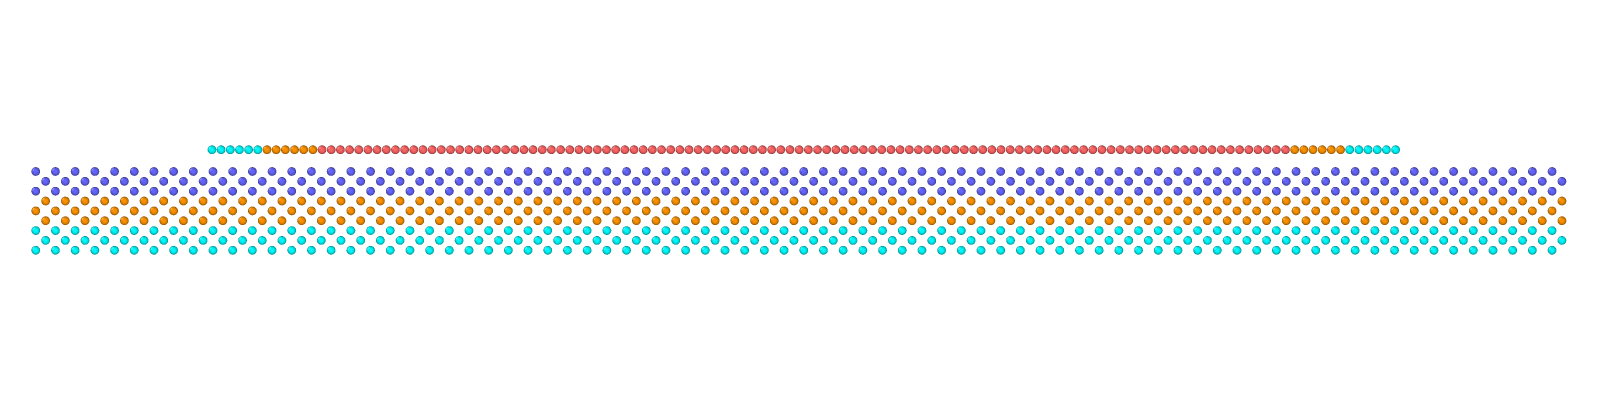
\includegraphics[width=\textwidth]{figures/system/system_sideview.png}
      \caption{}
      \label{fig:sideview}
  \end{subfigure}
  \hfill
  \begin{subfigure}[b]{0.70\textwidth}
      \centering
      \includegraphics[width=\textwidth]{figures/system/system_topview_anno.png}
      \caption{}
      \label{fig:topview}
  \end{subfigure}
  \hfill
     \caption{System configuration colorized to indicate NVE parts (red), thermostat parts (green) and rigid parts (blue). (a) Side view showing the sheet on top of the substrate. (b) Top view showing only the sheet.}
     \label{fig:system}
\end{figure}


\begin{figure}[H]
  \centering
  \includegraphics[width=0.80\linewidth]{figures/system/hon_stretch.png}
  \caption{Stretched Kirigami sheet against a substrate. The substrate is excluded from the image for better visibility. The atoms are colorized to indicate NVE parts (red), thermostat parts (green) and rigid parts (blue). The pattern used is the Honeycomb $(2,2,1,5)$ (see~\cref{chap:system}) at a 100\% strain level.}
  \label{fig:kirigami_stretch}
\end{figure}



\section{Numerical procedure}\label{sec:num_proc}
Following the system setup as described previously, the next step involves letting the system relax and reach a stable equilibrium. During this phase, slight modifications to the sheet-substrate distance and lattice spacing take place, both of which are influenced by the thermostat's target temperature. We then stretch the sheet to the desired length, apply normal load and finally slide it along the substrate. The full numerical procedure can be arranged into the following steps. Some steps have been given a default duration denoted in parentheses in units of ps, \num{e-12} seconds.
\begin{enumerate}
  \item \textbf{Relaxation} (\SI{15}{ps}): The sheet and substrate are relaxed for 
  \SI{15}{ps} after being added in their crystalline form with a separation distance of \SI{3}{\text{Å}}. Given that the equilibrium separation distance will vary with temperature, this value is based on an average estimate suiting our temperature range of interest. In order to avoid any sheet drift we constrain it with the use of three hard spring forces with a spring constant of
  $\SI{e5}{eV/\text{Å}^2} \sim \SI{1.6e6}{N/m}$: One spring attaches the sheet center of mass (\acrshort{CM}) to its original position, preventing \acrshort{CM} drift, while the remaining two springs are attached to the pull blocks \acrshort{CM}, to prevent rotation. In principle, fixing only one of the pull blocks would suffice, but we choose to fixate both to maintain symmetry. During the relaxation phase, we consider the pull blocks to be rigid with respect to the z-direction only (perpendicular to the sheet). That is, all the forces in the z-direction are summed up and applied as a uniform external force, while the pull blocks are free to expand and contract in the x-y-plane. This feature is incorporated to allow the pull blocks to readjust the lattice spacing according to the temperature of the system. For the following steps, the pull blocks are made truly rigid with respect to all directions, and the spring forces are terminated. 
  \item \textbf{Stretch}: To stretch the sheet, the two opposing rigid parts of the pull blocks are moved apart at a constant velocity until the desired strain level is achieved. The duration of this phase is determined by the values of the \textit{strain speed} and \textit{strain amount} parameters.
  \item \textbf{Pause} (\SI{5}{ps}): The sheet is further relaxed for \SI{5}{ps} to ensure that the sheet is stable and equilibrated after the applied strain deformation. 
  \item \textbf{Normal load} (\SI{5}{ps}): The pull blocks are subjected to a uniformly applied load in the negative z-direction, thereby pushing the sheet perpendicularly into the substrate. Initially a viscous damping force, $F = -\gamma \vec{v}$ with damping factor $\gamma$ and velocity $\vec{v}$, is added to resist rapid acceleration of the sheet and prevent a hard impact between the sheet and substrate as the sheet-substrate distance decreases. The damping coefficient is set to $\gamma = \SI{8e-4}{nN/(m/s)}$ and terminated after \SI{0.5}{ps} which was found to be suitable for the extreme load cases of our intended range. The remaining \SI{4.5}{ps} is devoted to further relaxation in order to reach a sheet-substrate distance equilibrium.
  \item \textbf{Sliding}: A virtual atom is introduced into the simulation which
  exclusively interacts with the rigid parts of the pull blocks through a spring force with spring constant $K$ in the x-y-plane. The force in the z-direction is not influenced by the spring force and is instead governed by the equilibrium between the normal load and the normal force response from the sheet-substrate interaction. The virtual atom is immediately given a constant velocity, given by the \textit{sliding speed} parameter. This results in an initial linear increase in sliding force proportional to sliding speed and spring constant $F_{\textit{slide}} \propto Kvt$. An infinite spring constant can also be enforced for which the spring is omitted and the pull blocks are moved rigidly with a constant speed.
\end{enumerate}
To limit the complexity of the friction behavior we want to consider systems without wear. To make sure that no wear is taking place for the sheet, we monitor the nearest neighbors for each atom throughout the simulation. At the initial timestep the three nearest neighbors, sitting at a distance \SI{1.42}{\text{Å}}, of all graphene atoms are recorded. If any of these nearest neighbors exceeds a threshold distance of \SI{4}{\text{Å}}, indicating a bond breakage, this is marked as a rupture and we halt the simulation. By conducting several test simulations involving high loads and high sliding speeds, we have visually confirmed that no wear occurs in the substrate, which demonstrates significantly greater wear resistance than the sheet. Therefore, we concluded that it was unnecessary to monitor the substrate for any signs of wear during the simulations.


\section{Setting up the substrate}\label{sec:substrate}
The substrate is created as a rectangular slab of silicon (Si). We create the
initial configuration according to its crystalline structure given as a diamond
cubic crystal with a lattice parameter $a_{\text{Si}} = \SI{5.43}{\text{Å}}$.
The default substrate thickness is chosen such that 9 layers of atoms appear (2
unit cells) corresponding to a thickness of \SI{10.86}{\text{Å}}. The x-y
dimensions are chosen to match the dimensions of the sheet. That is, we define a
margin between the sheet edge and the substrate edge for the x- and y-direction
respectively. Since we use periodic boundary conditions a too small margin would
result in the sheet edges interacting with themselves through the boundary. The
absolute lower limit for the margin choice is half the cut-off distance for
the Tersoff potential, governing the graphene sheet interaction, at $R + D =
\SI{2.1}{\text{Å}}$. However, due to fluctuations in the sheet, we cannot set the margin too
close to that limit. In addition, we need to consider the buckling of the sheet as it is stretched, which might cause an expansion in the x-direction for certain configurations. We choose an x-margin of \SI{20}{\text{Å}} which provides $2\cdot
\SI{20}{\text{Å}} - \SI{2.1}{\text{Å}} = \SI{37.9}{\text{Å}}$ of additional
spacing with respect to the absolute lower limit. By looking over the simulation
result visually we confirm that this leaves more than enough room in the cases
of most buckling. For the y-direction the rigid parts of the pull-blocks
moves a certain distance based on the strain value exclusively, and we define
the y-margin based on the remaining distance to the edge after stretching.
However, as the sheet travels through the periodic boundaries in the y-direction
when sliding, we want to add some additional spacing through the y-margin in
order to let the substrate surface relax before interacting with the sheet a
second time. We choose a y-margin of \SI{15}{\text{Å}} for which the preferred sliding speed
of $\SI{20}{m/s} = \SI{0.2}{\text{Å}/ps}$ gives \SI{150}{ps} of relaxation time
between encounters with the sheet. 


\section{Setting up sheet}
The sheet consists of graphene, which is a single layer of carbon atoms arranged in a hexagonal lattice structure. The bulk version of graphene is graphite and is a stacked structure of multiple graphene layers. 

\begin{multicols}{2}
We can describe the graphene 2D crystal structure in terms of its primitive lattice vectors $\vec{a_1}$ and $\vec{a_2}$ and a basis. The basis describes the atoms associated with each lattice site, and we populate the lattice by translating the basis by any linear combination of the lattice vectors 
\begin{align*}
  \vec{T}_{mn} = m\vec{a_1} + n\vec{a_2}, \qquad m,n \in \mathbb{N}.
\end{align*}
For graphene, we have the primitive lattice vectors~\cite{gray2009crystal} 
\begin{align}
  \vec{a_1} &= a \left(\frac{\sqrt{3}}{2}, -\frac{1}{2}\right), \qquad \vec{a_2} = a \left(\frac{\sqrt{3}}{2}, \frac{1}{2}\right), \label{eq:prim_vec} \\
  |\vec{a_1}| &= |\vec{a_2}| = a = 2.46 \ \text{Å}. \nonumber
\end{align}
Notice that we deliberately excluded the third coordinate as we only consider a
single graphene layer and thus we do not have to consider the stacking structure of 3D graphite. The basis consists of two carbon atoms given as 
\begin{align}
  \Big\{\Big(0,0\Big), \frac{a}{2}\Big(\frac{1}{\sqrt{3}}, 1 \Big) \Big\}.
  \label{eq:basis}
\end{align}
The crystal structure is visualized in~\cref{fig:graphene_crystal}. The hexagonal lattice structure makes for equal spacing between all pairs of atoms with an interatomic distance
\begin{align*}
  \left|\left|\frac{a}{2}\Big(\frac{1}{\sqrt{3}}, 1 \Big)\right|\right| \approx 1.42 \ \text{Å}.
\end{align*}
  
\begin{figure}[H]
  \centering
  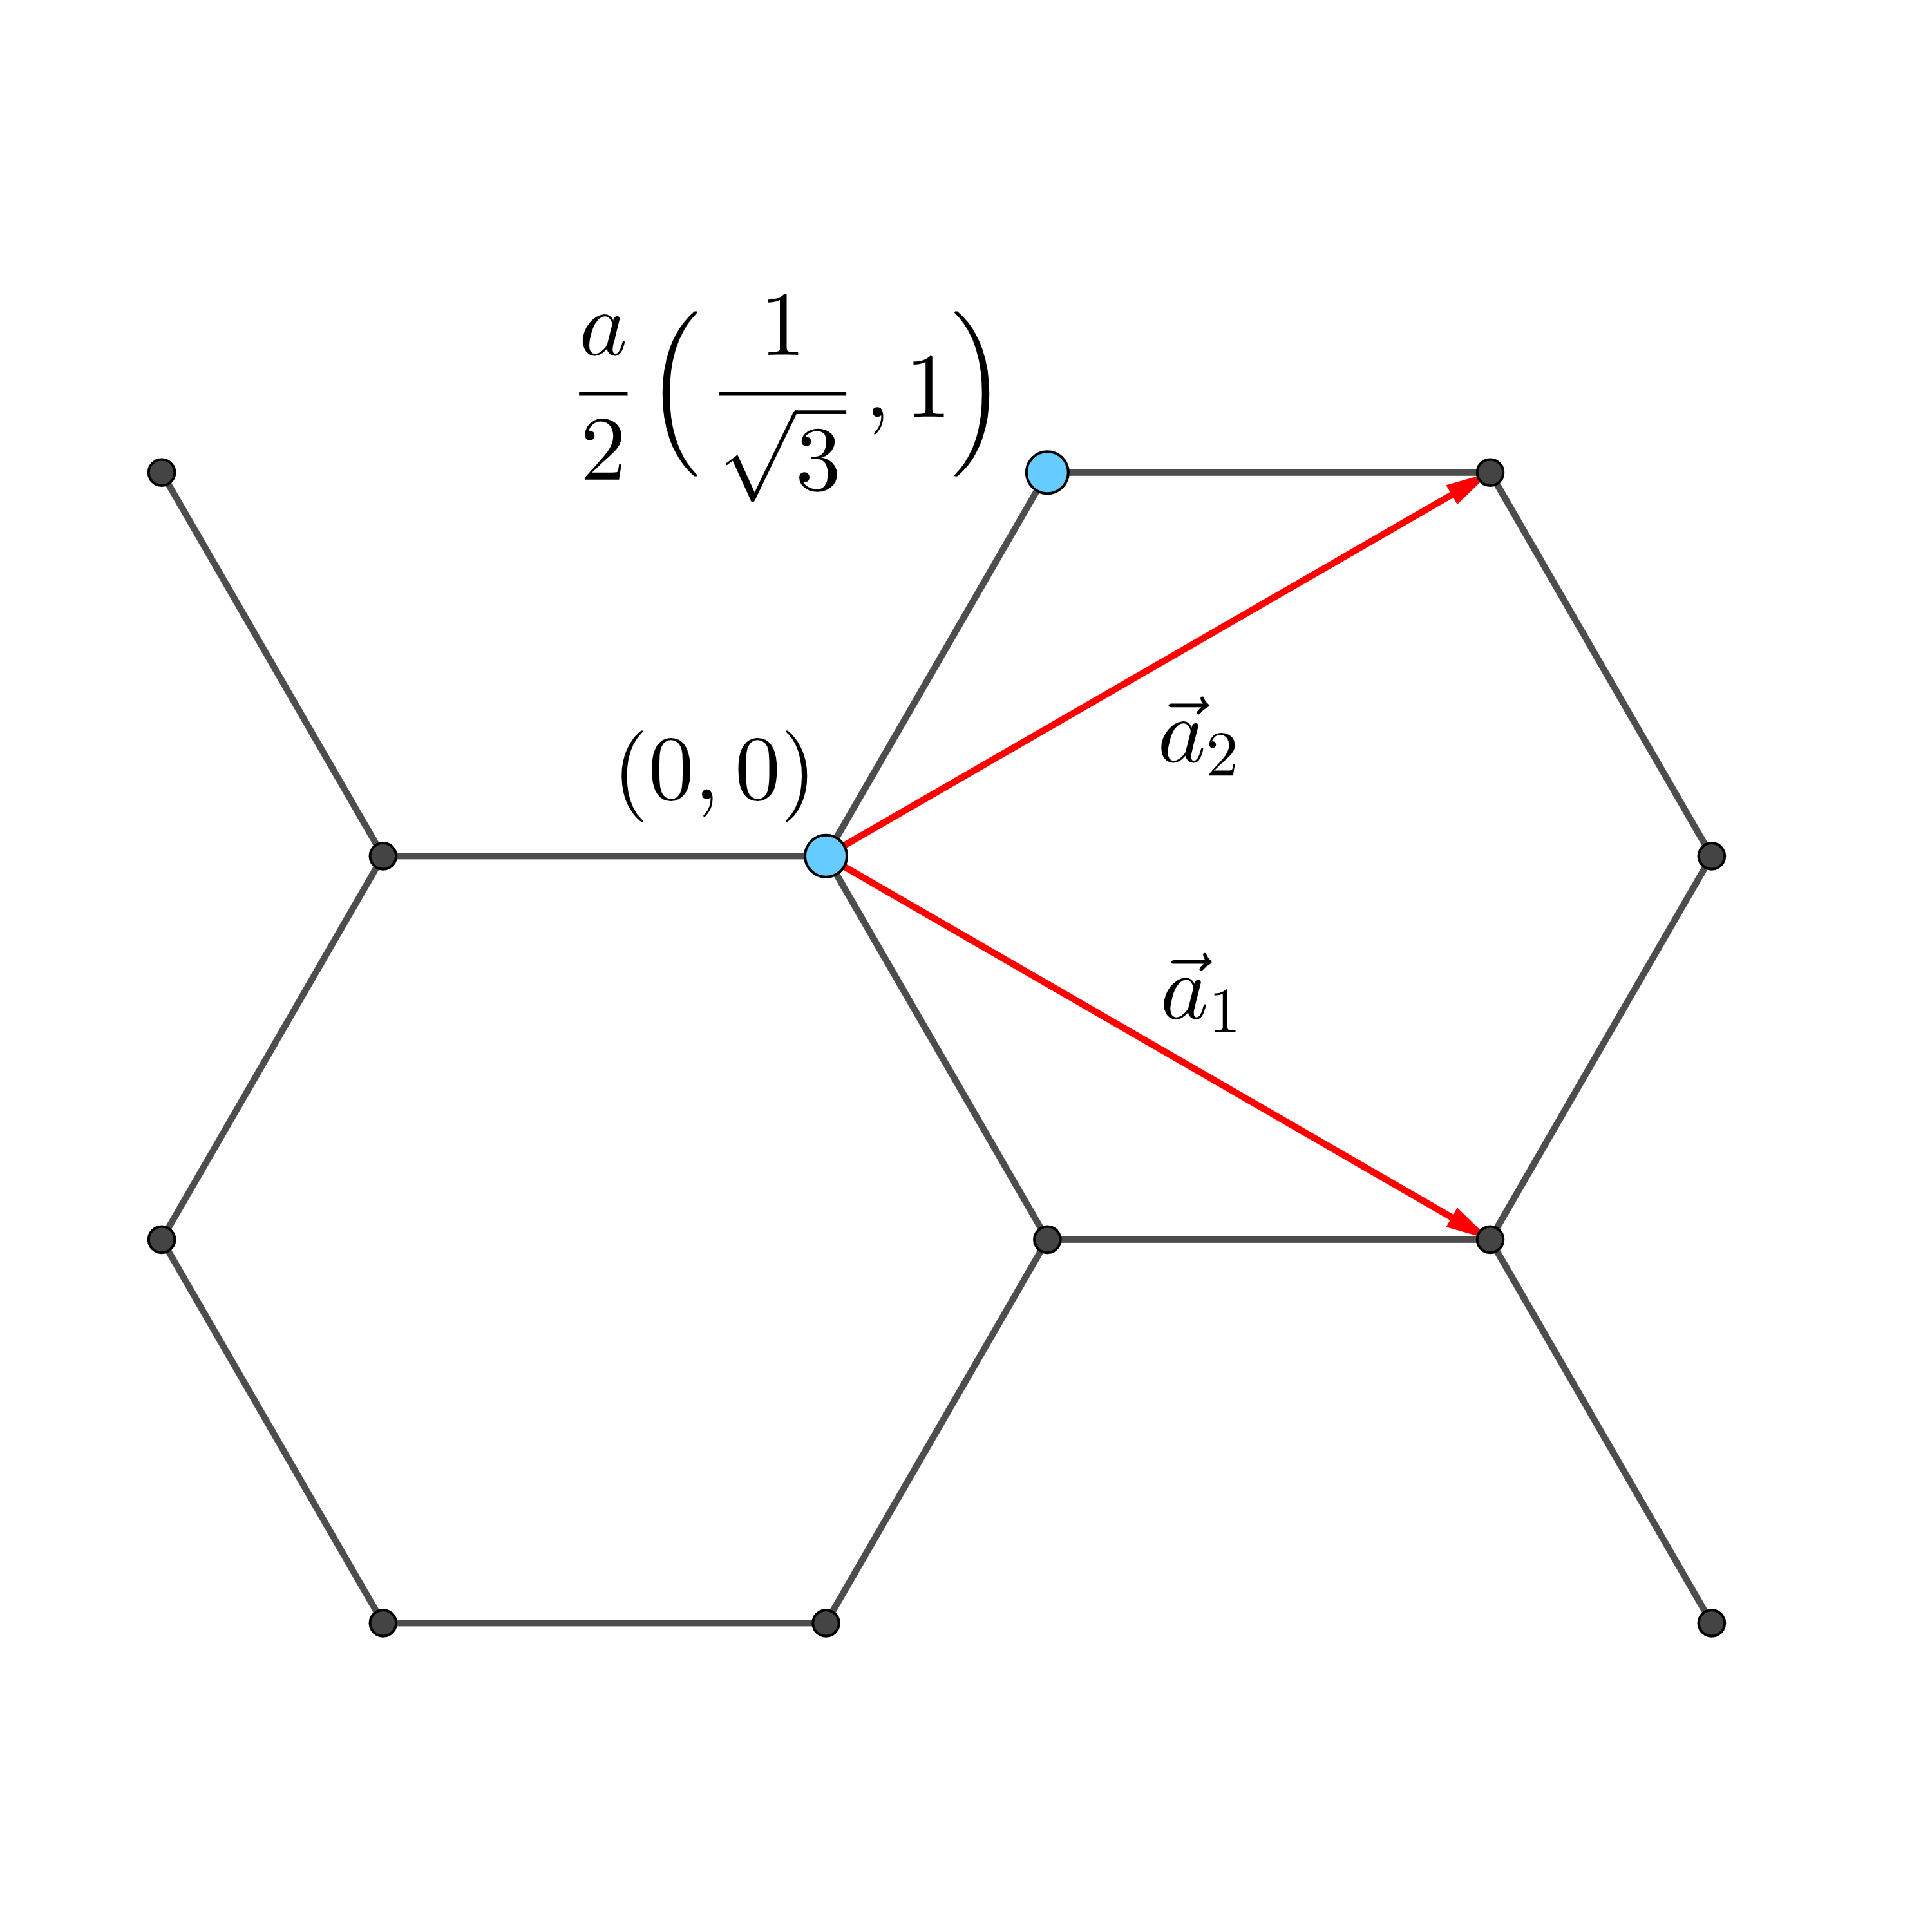
\includegraphics[width=0.9\linewidth]{figures/system/crystal.png}
  \caption{Illustration of the graphene crystal structure. The dots represent atom sites whereas blue dots denote the basis atoms (\cref{eq:basis}). The red arrows denote the primitive lattice vectors (\cref{eq:prim_vec}). }
  \label{fig:graphene_crystal}
\end{figure}
  
\end{multicols}



\subsection{Indexing}
In order to describe the Kirigami cut patterns applied to the graphene sheet we require an indexing system that provides a unique representation of the atoms in the lattice. This allows us to represent the pattern as a binary matrix, where 0 denotes removed atoms and 1 denotes present atoms. We let the x-coordinate correspond to the so-called \textit{armchair} direction of the sheet and the y-coordinate to the so-called \textit{zigzag} direction. Notice that the x-coordinate will point to \textit{zigzag} chains of atoms for which the starting point $(x, 0)$ is not evenly spaced as illustrated in~\cref{fig:atom_indexing}. Other
solutions might naturally involve the lattice vectors, but since these are used
to translate between similar basis atoms it introduces an unfortunate duality as
one would then need to include the basis atom of choice into the indexing system
as well. Additionally, we want an indexing system that conserves the relative
physical position of neighbors. That is, atom $(i, j)$ should be in the
proximity of $\{(i+1, j), (i-1, j), (i, j+1), (i, j-1)\}$. However, due to the
hexagonal structure of the lattice, only three said neighbor indexes will be
actual nearest neighbors in the lattice. While $(i, j\pm 1)$ is always the nearest
neighbor, the index of the nearest neighbor in the x-direction oscillates for
each incrementing of the x- or y-coordinate. That is, the nearest neighbors \acrshort{NN} are decided as
\begin{equation}
  \begin{aligned}
    (i + j) \ \text{is even} &\rightarrow \text{\acrshort{NN}} = \{(i-1, j), (i, j+1), (i, j-1)\}, \\
    (i + j) \ \text{is odd} &\rightarrow \text{\acrshort{NN}} = \{(i+1, j), (i, j+1), (i, j-1)\}.
  \end{aligned}
  \label{eq:atom_neigh_idx}
\end{equation}
We can visually verify this by consulting~\cref{fig:atom_indexing}, which shows that the nearest neighbor indexes depend on whether the atom is oriented to the left or right side in the zigzag chain.

\begin{figure}[!htb]
  \centering
  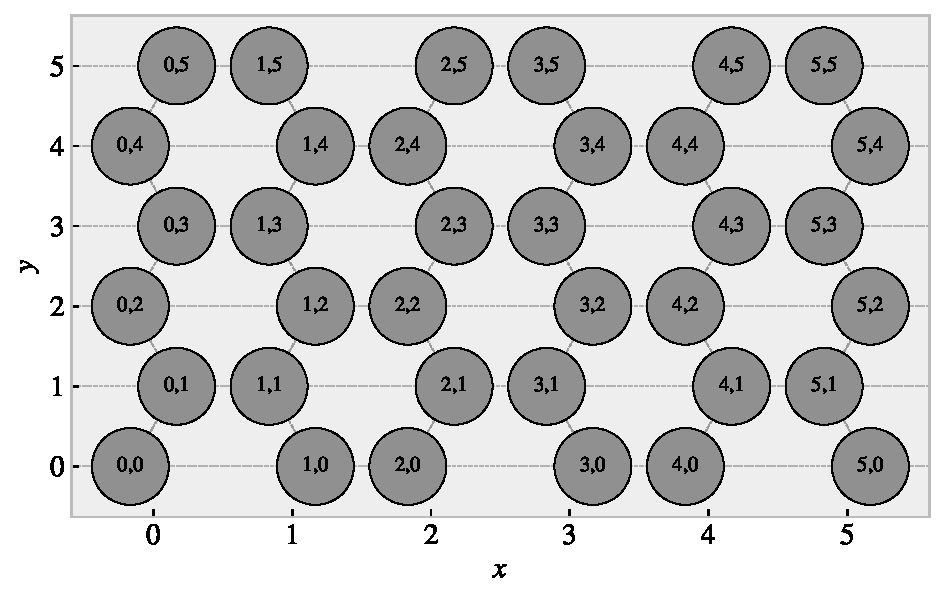
\includegraphics[width=0.7\linewidth]{figures/system/atom_indexing.pdf}
  \caption{Illustration of the graphene atom site indexing. The x-coordinate increment along the armchair direction (pointing to zigzag chains) while the y-coordinate increment along the zigzag direction.}
  \label{fig:atom_indexing}
\end{figure}


\subsection{Removing atoms}
To simplify the formulation of the cut patterns, we introduce the \textit{center element} which is placed in each gap of the hexagonal honeycomb structure as shown in~\cref{fig:center_indexing}. These are not populated by any atoms but will serve as a reference for the numerical approaches to defining a cut pattern.

\begin{figure}[!htb]
  \centering
  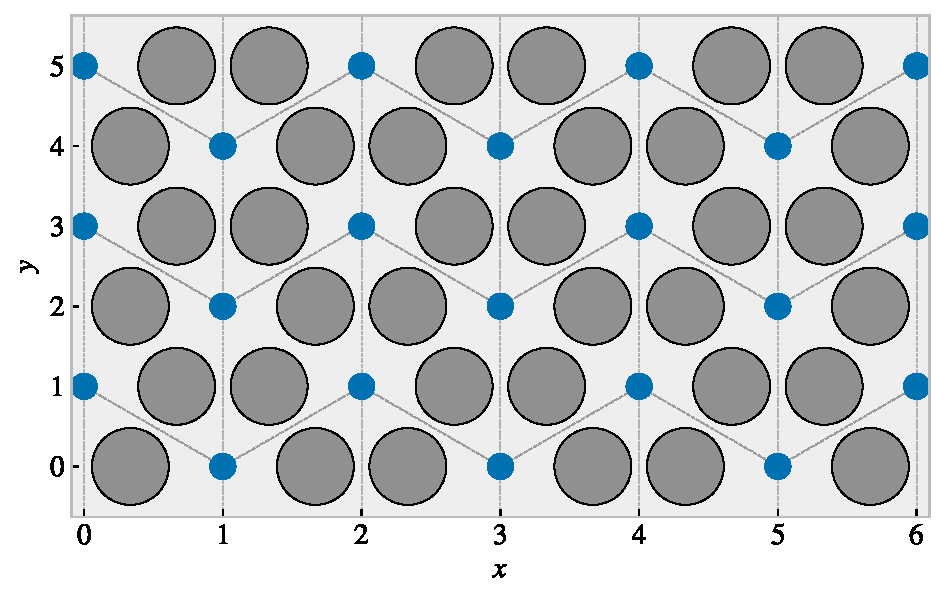
\includegraphics[width=0.7\linewidth]{figures/system/center_indexing.pdf}
  \caption{Illustration of the indexing for the introduced center elements depicted with blue circles placed in the gap of the honeycomb structure laid out by the graphene sheet atoms depicted with grey circles. The y-coordinate increment along the zigzag direction (pointing to armchair chains) while the x-coordinate increment along the armchair direction.}
  \label{fig:center_indexing}
\end{figure}

The nearest neighbors of the center element alternate with position, similar to the atom site indexing. However, this time it is only dependent on the x-coordinate position. Each center element has six nearest neighbors, in a clockwise
direction we can denote them: ``up'', ``upper right'', ``lower right'',
``down'', ``lower left'', ``upper left''. The ``up'' and ``down'' neighbors are always accessible as $(i,j\pm 1)$. However, for even $i$ the $(i+1,j)$ index corresponds to the
``lower right'' neighbour while for odd $i$ this corresponds to the ``upper
right'' neighbour. This shifting applies for all left- or right-oriented neighbors and the full neighbor list is illustrated in~\cref{fig:center_directions}. Analog to the case of atom site indexing, we notice that the nearest neighbor indexes depend on whether the center element is oriented up or down on the armchair chain.

\begin{figure}[!htb]
  \centering
  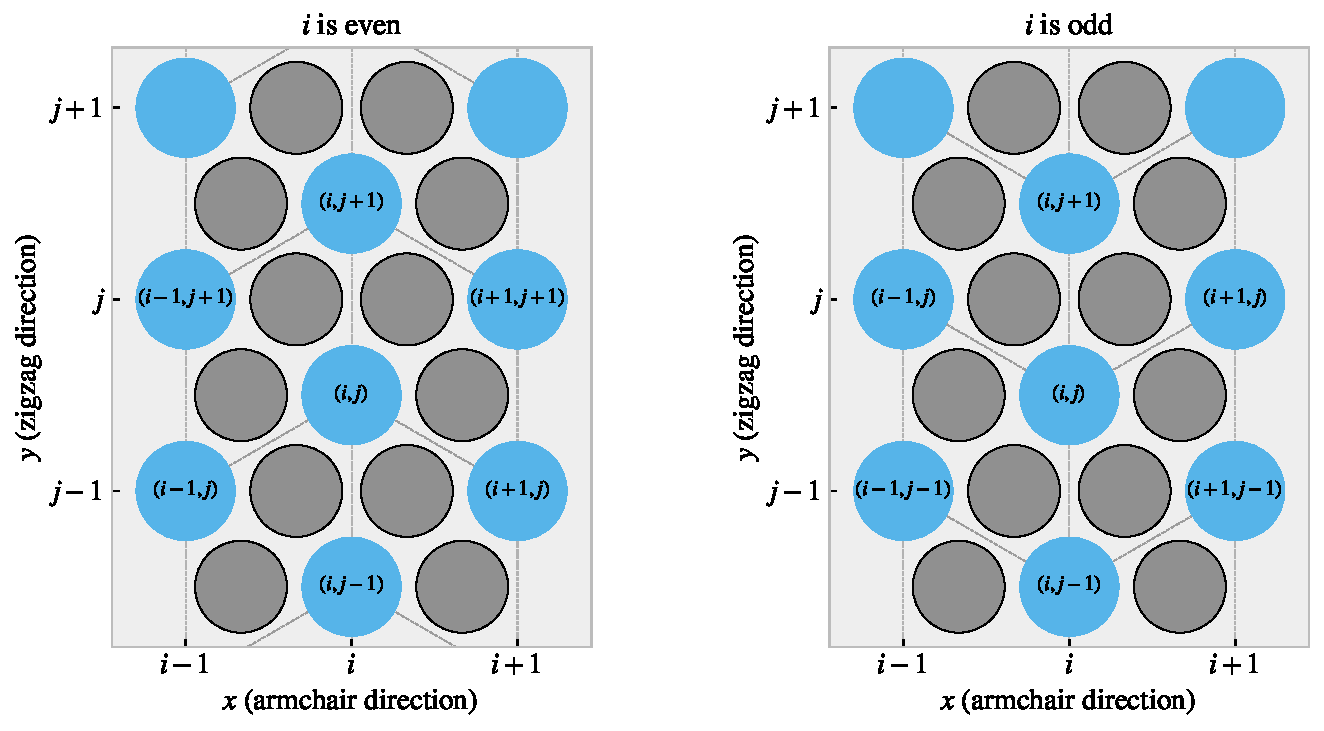
\includegraphics[width=0.70\linewidth]{figures/system/center_directions.pdf}
  \caption{Illustration of the center element neighbor indexes for the case when the x-coordinate $i$ is even (left) and $i$ is odd (right).}
  \label{fig:center_directions}
\end{figure}

We define a cut pattern by a connected path of center elements. As
we walk between center elements through nearest neighbor walking we can remove atoms according to one of two rules 
\begin{enumerate}
  \item Remove intersecting atoms: We remove the pair of atoms placed directly
  in the path we are walking. That is, when jumping to the ``up'' center
  element we remove the two upper atoms located in the local hexagon of atoms.
  This method is sensitive to the order of the center elements in the path. 
  \item Remove all surrounding atoms: We simply remove all atoms in the local
  hexagon surrounding each center element. This method is independent of the
  ordering of center elements in the path.
\end{enumerate}
We notice that removing atoms using either of these rules will not guarantee an injective, one-to-one, mapping. The first rule, being path dependent, will more often result in a unique result. However, for both methods, it is possible to construct two different paths leading to the same cut pattern as shown in the following example:
\begin{align*}
  \text{Path 1:} \quad (i, j) &\rightarrow \underbrace{(i+1,j+1)}_{\text{upper right}} \rightarrow \underbrace{(i, j+1)}_{\text{up}} \rightarrow \underbrace{(i+1, j+2)}_{\text{upper right + up}} \rightarrow \underbrace{(i+1, j+1)}_{\text{upper right}} \\
  \text{Path 2:} \quad (i, j) &\rightarrow \underbrace{(i+1,j+1)}_{\text{upper right}} \rightarrow \underbrace{(i+1, j+2)}_{\text{upper right + up}} \rightarrow \underbrace{(i, j+1)}_{\text{up}}
\end{align*}
For the second rule, it is even more obvious that different paths can result in the same final pattern. For instance, if we incircle a center element completely there will be no surrounding atoms left to remove when jumping to that center element. This highlights the motivation for defining the atom-based indexing system which yields an injective mapping between the binary matrix and the graphene lattice cut pattern. However, using the center elements as a reference makes it easier to design the cut patterns since we can always go in one of the six directions defined by the center element neighbors. In contrast, the atom indexing system has alternating directions for its neighbors, which makes it more involved to define cut patterns.


\section{Kirigami patterns}
We propose a series of Kirigami-inspired cut patterns for the altering of the graphene sheet. We seek inspiration from macroscale patterns that showcase a considerable amount of out-of-plane buckling when stretched. We choose to imitate two different designs: 1) An alternating repeating series of perpendicular cuts as shown in~\cref{fig:kirigami_inspiration_a} popularly used in studies of morphable metematerials~\cite{new_pop_up}. This pattern produces surface buckling with a tetrahedron (three-sided pyramid) shape when stretched. 2) A more intricate pattern shown in~\cref{fig:kirigami_inspiration_b} which is used commercially by Scotch\textsuperscript{TM} Cushion Lock\textsuperscript{TM}~\cite{cushion_wrap} as protective wrap for items during shipping. This pattern buckles into a hexagonal honeycomb structure when stretched. In addition to the modeling of the so-called \textit{Tetrahedron} and \textit{Honeycomb} patterns, we also create a series of random walk patterns.

\begin{figure}[!htb]
  \centering
  \begin{subfigure}[t]{0.48\textwidth}
      \centering
      \includegraphics[width=\textwidth]{figures/system/pop_up_inspiration.png}
      \caption{}
      \label{fig:kirigami_inspiration_a}
    \end{subfigure}
    \hfill
    \begin{subfigure}[t]{0.48\textwidth}
      \centering
      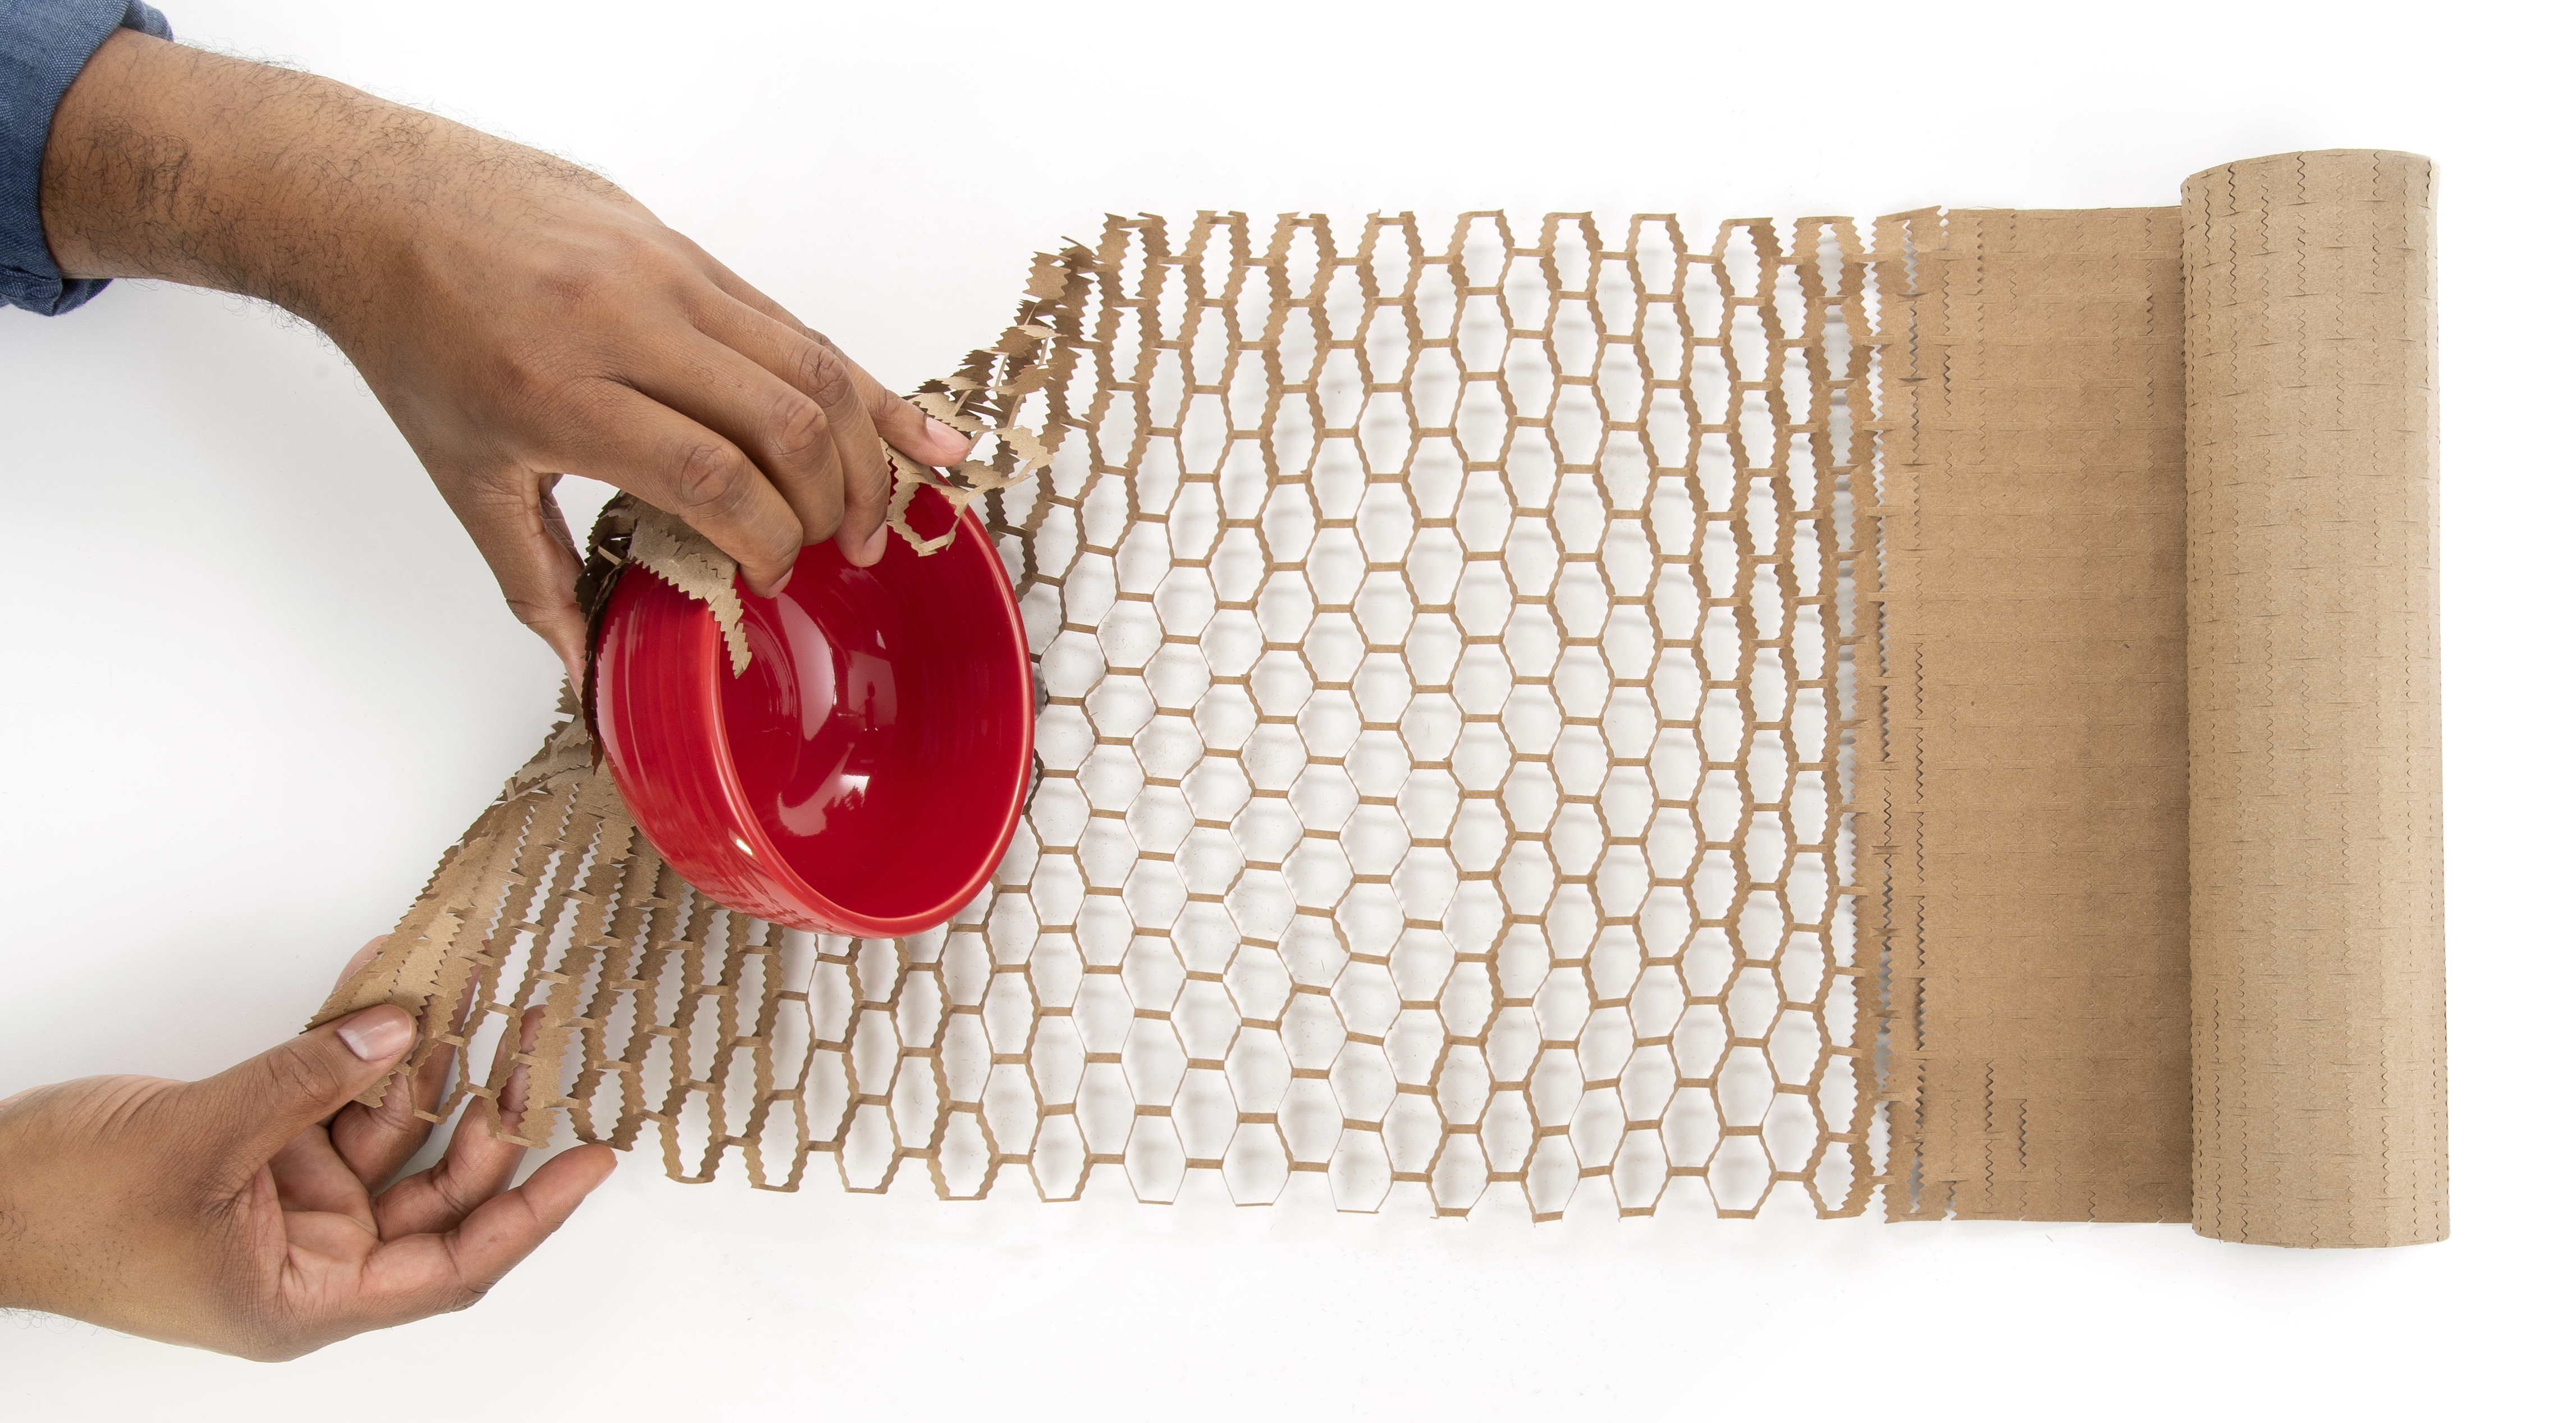
\includegraphics[width=\textwidth]{figures/system/honeycomb_inspiration.jpg}
      \caption{}
      \label{fig:kirigami_inspiration_b}
  \end{subfigure}
  \hfill
     \caption{Macroscale kirigami cut patterns used as inspiration for the nanoscale implementation. (a) Tetrahedron: Alternating perpendicular cuts producing a tetrahedron-shaped surface buckling when stretched. Reproduced from~\cite{new_pop_up}. (b) Honeycomb: Scotch\textsuperscript{TM} Cushion Lock\textsuperscript{TM}~\cite{cushion_wrap} producing a honeycomb-shaped surface buckling when stretched. Reproduced from~\cite{cushion_wrap}.}
     \label{fig:kirigami_inspiration}
\end{figure}

\subsection{Tetrahedron}
The \textit{Tetrahedron} pattern is defined in terms of center elements for
which all atoms surrounding a given center element are removed. The pattern
consists of two straight cuts, referred to as line 1 and line 2, that are
arranged perpendicular to each other. The lines are positioned such that the
center of one line aligns with the end of the other line, and with a given spacing in
between (see~\cref{fig:pop_up}). In order to achieve
perpendicular cuts we cannot rely purely on the six center element directions
corresponding to the center element neighbors which are spaced by 60$^\circ$. We
let line 1 run along the center elements in the direction of the ``upper right''
(and ``lower left'') center elements, while line 2 goes in the direction between
the ``down'' and ``lower right'' (``up'' and ``upper left'') center elements,
corresponding to the direction $(1/\sqrt{3}, -1)$. We define variations of the
pattern by the number of center elements $L_1$ and $L_2$ in line 1 and 2
respectively, together with the spacing between the lines $d$, as the tuple
$(L_1, L_2, d)$. The pattern is constructed by translating the two lines to the
whole sheet according to the spacing. Due to the alignment criteria of having
one line point to the center of the other line, we can only allow an odd line
length. Furthermore, in order to ensure that each center element is translated
to an $i$-index of similar odd or evenness, we must in practice require that
$|L_2 - L_1| = 2, 6, 10, \ldots \ $. \cref{fig:pop_up} shows a visual
representation of the pattern components for the $(7, 5, 2)$ patteren. 


\begin{figure}[!htb]
  \centering
  \begin{subfigure}[t]{0.49\textwidth}
      \centering
      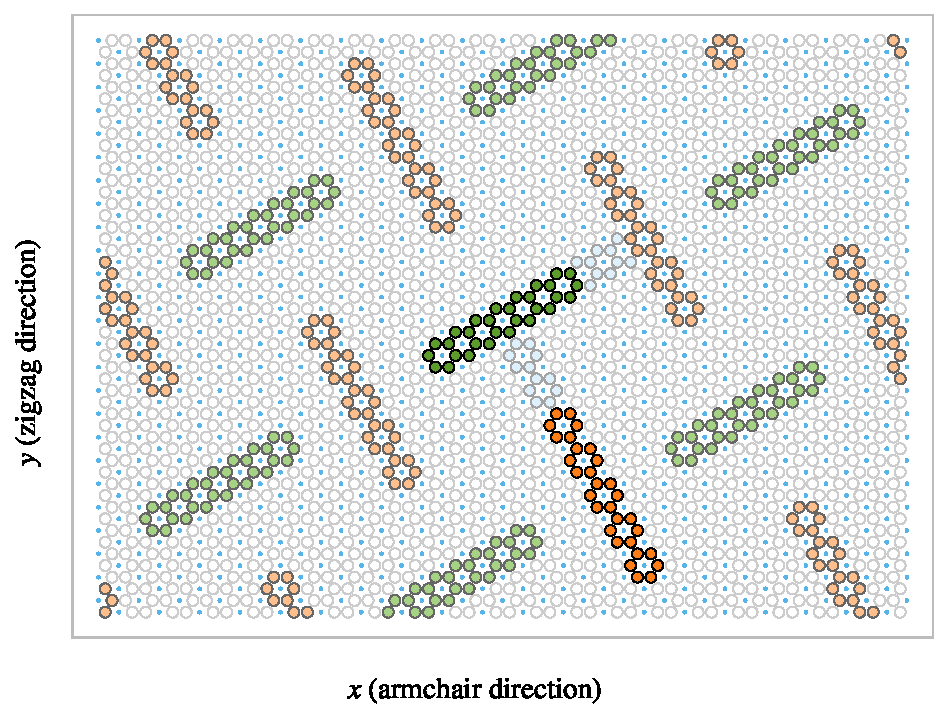
\includegraphics[width=\textwidth]{figures/system/pop_up_inverse.pdf}
      \caption{}
      \label{fig:pop_up_a}
    \end{subfigure}
    \hfill
    \begin{subfigure}[t]{0.49\textwidth}
      \centering
      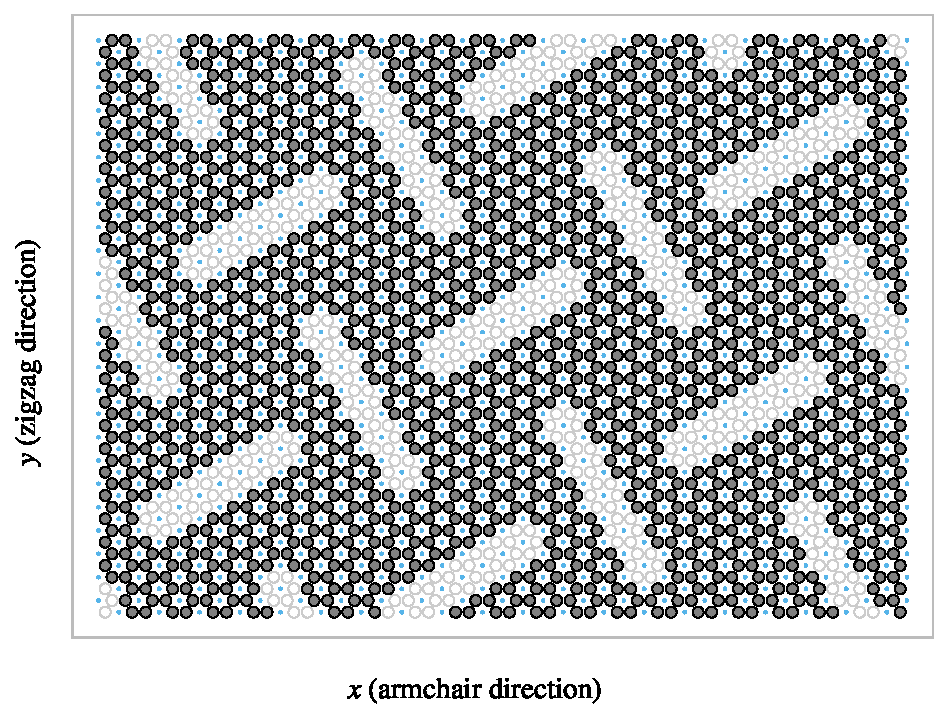
\includegraphics[width=\textwidth]{figures/system/pop_up_pattern.pdf}
      \caption{}
      \label{fig:pop_up_b}
  \end{subfigure}
  \hfill
     \caption{Visual representation of the Tetrahedron pattern consisting of two perpendicular lines, line 1 and line 2, of length $L_1$ and $L_2$ respectively, with spacing $d$. This example uses $(L_1, L_2, d) = (7, 5, 2)$ and a sheet matrix size $40 \times 50$ corresponding to 2000 atom sites and an approximate sheet size of $84 \times \SI{77}{\text{Å}}$. The non-filled circles represent the possible atom site positions and the blue dots are the center elements. (a) Highlights the removed atoms in the pattern. Line 1 is shown in green and line 2 in orange, with lighter colors for the translated variations. The spacing is indicated in light blue. (b) The sheet after applying the cut pattern with grey circles denoting present atoms.}
     \label{fig:pop_up}
\end{figure}


\begin{figure}[!htb]
  \centering
  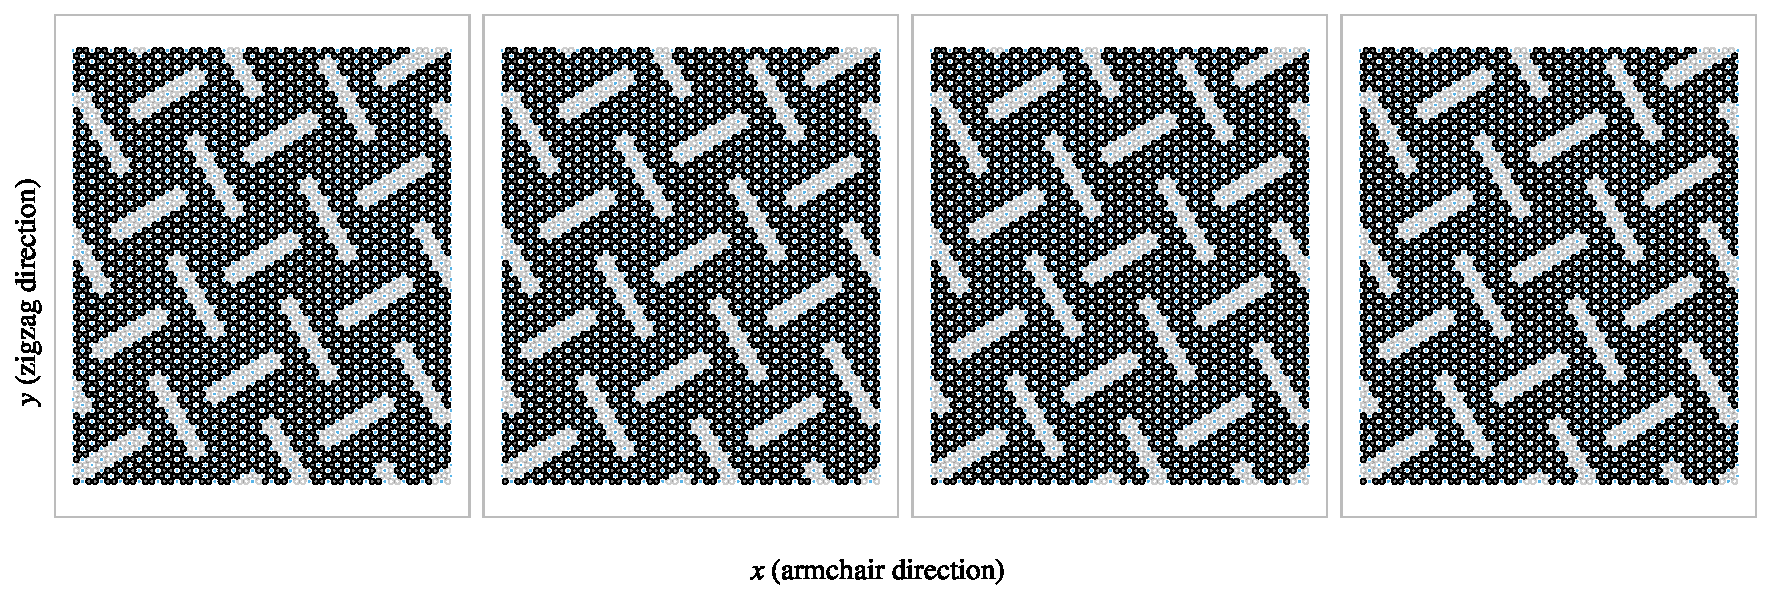
\includegraphics[width=\linewidth]{figures/system/pop_up_flavors.png}
  \caption{Example of different Tetrahedron cut pattern variations. The specific parameters are noted as titles and all of the patterns use the center of the sheet as a reference position. The circles in the figure represent atom sites, where grey-filled circles indicate the presence of atoms and transparent circles indicate removed atoms. The blue dots in the figure indicate the center elements. The sheet matrix size is $40 \times 80$ corresponding to 3200 atom sites and an approximate sheet size of $84 \times \SI{123}{\text{Å}}$.}
  \label{fig:pop_up_flavors}
\end{figure}

In addition to the three parameters $L_1, L_2, d$, the pattern is also anchored
to a reference point that describes the position of line 1 and line 2 before
being translated to span the sheet. Due to the repeating structure of the
pattern, there exist a small finite number of unique reference positions. For
the pattern $(7, 5, 2)$ used as an example in~\cref{fig:pop_up}, there are
140 unique reference points\footnote{The general formula for calculating this number is rather
complicated in comparison to its importance in this context. Therefore, we have
omitted the formula and only provide the numerically backed result for the
specific parameter set. The derivation of the formula was also deemed not to be
rigorous enough.}. Some additional variation of the
pattern is showcased in~\cref{fig:pop_up_flavors} each with a reference position
at the center of the sheet. Note that a smaller sheet size than used in the simulations is used in
both~\cref{fig:pop_up} and~\cref{fig:pop_up_flavors} for illustrative purposes.



\subsection{Honeycomb}
The \textit{Honeycomb} pattern is defined, similarly to the Tetrahedron pattern,
in terms of the center elements for which all surrounding atoms are removed. The
Honeycomb pattern is built from a repeating series of cuts reminiscent of the
Roman numeral one rotated by 90$^{\circ}$
(\rotatebox[origin=c]{90}{\MakeUppercase{\romannumeral 1}}). For a given spacing
these are put next to each other in the x-direction,
\rotatebox[origin=c]{90}{\MakeUppercase{\romannumeral 1}}
\rotatebox[origin=c]{90}{\MakeUppercase{\romannumeral 1}}
\rotatebox[origin=c]{90}{\MakeUppercase{\romannumeral 1}}, to achieve a row
where only a thin \textit{bridge} in between is left to connect the sheet
vertically in the y-direction. By placing multiple rows along the y-direction
with alternating x-offset, we get the class of honeycomb patterns as visualized
in~\cref{fig:honeycomb}. The pattern is described in terms of the parameters:
(x-width, y-width, bridge thickness, bridge length) which is annotated
in~\cref{fig:honeycomb_a} with the parameters (2, 2, 1, 5) used as an example.
Some additional variations of the pattern class are showcased
in~\cref{fig:honeycomb_flavors}.


\begin{figure}[!htb]
  \centering
  \begin{subfigure}[t]{0.48\textwidth}
      \centering
      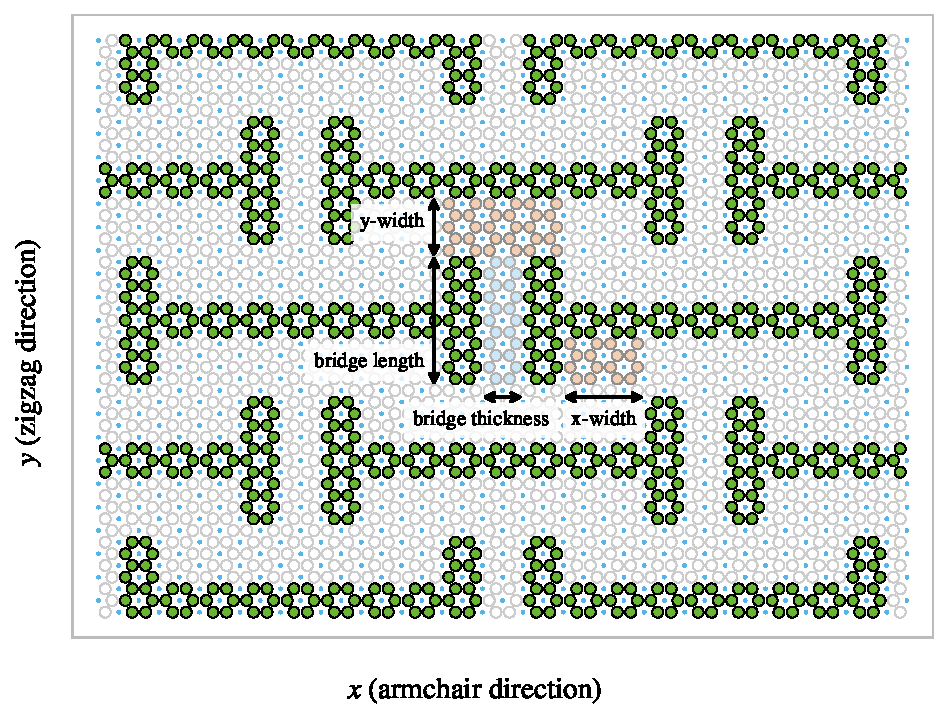
\includegraphics[width=\textwidth]{figures/system/honeycomb_inverse.pdf}
      \caption{}
      \label{fig:honeycomb_a}
    \end{subfigure}
    \hfill
    \begin{subfigure}[t]{0.48\textwidth}
      \centering
      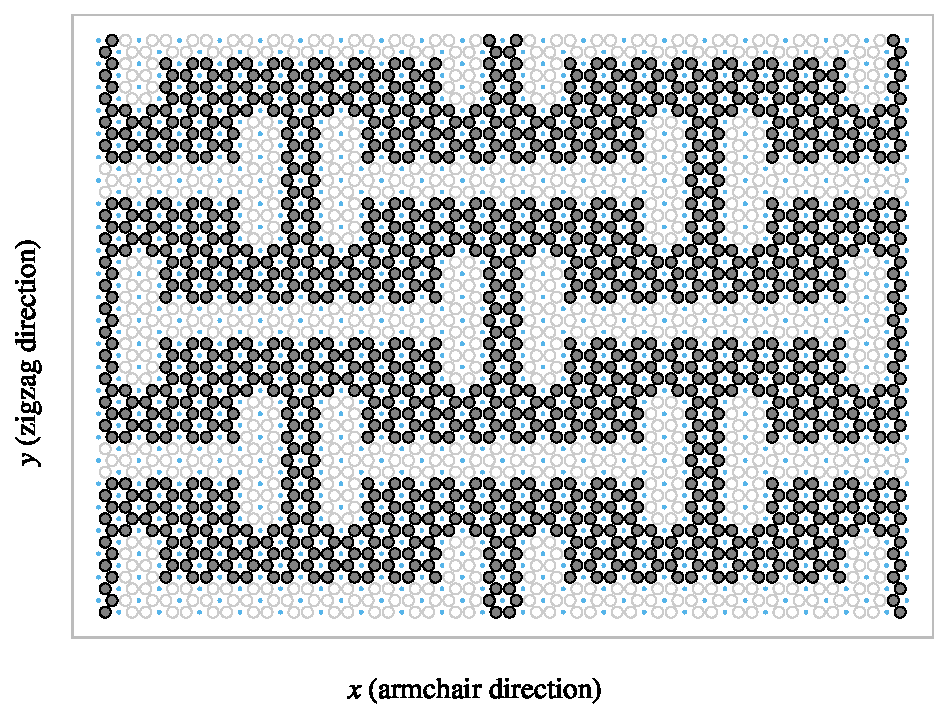
\includegraphics[width=\textwidth]{figures/system/honeycomb_pattern.pdf}
      \caption{}
      \label{fig:honeycomb_b}
  \end{subfigure}
  \hfill
     \caption{Visual representation of the Honeycomb pattern defined by the (x-width, y-width, bridge thickness, bridge length) parameters as annotated in panel (a). This example uses the parameters $(2,2,1,5)$ and a sheet matrix size $40 \times 50$ corresponding to 2000 atom sites and an approximate sheet size of $84 \times \SI{77}{\text{Å}}$. The non-filled circles represent the possible atom site positions and the blue dots are the center elements. (a) Highlights the removed atoms in the pattern with annotations for the four defining parameters. (b) The sheet after applying the cut pattern with grey circles denoting present atoms. }
     \label{fig:honeycomb}
\end{figure}


\begin{figure}[H]
  \centering
  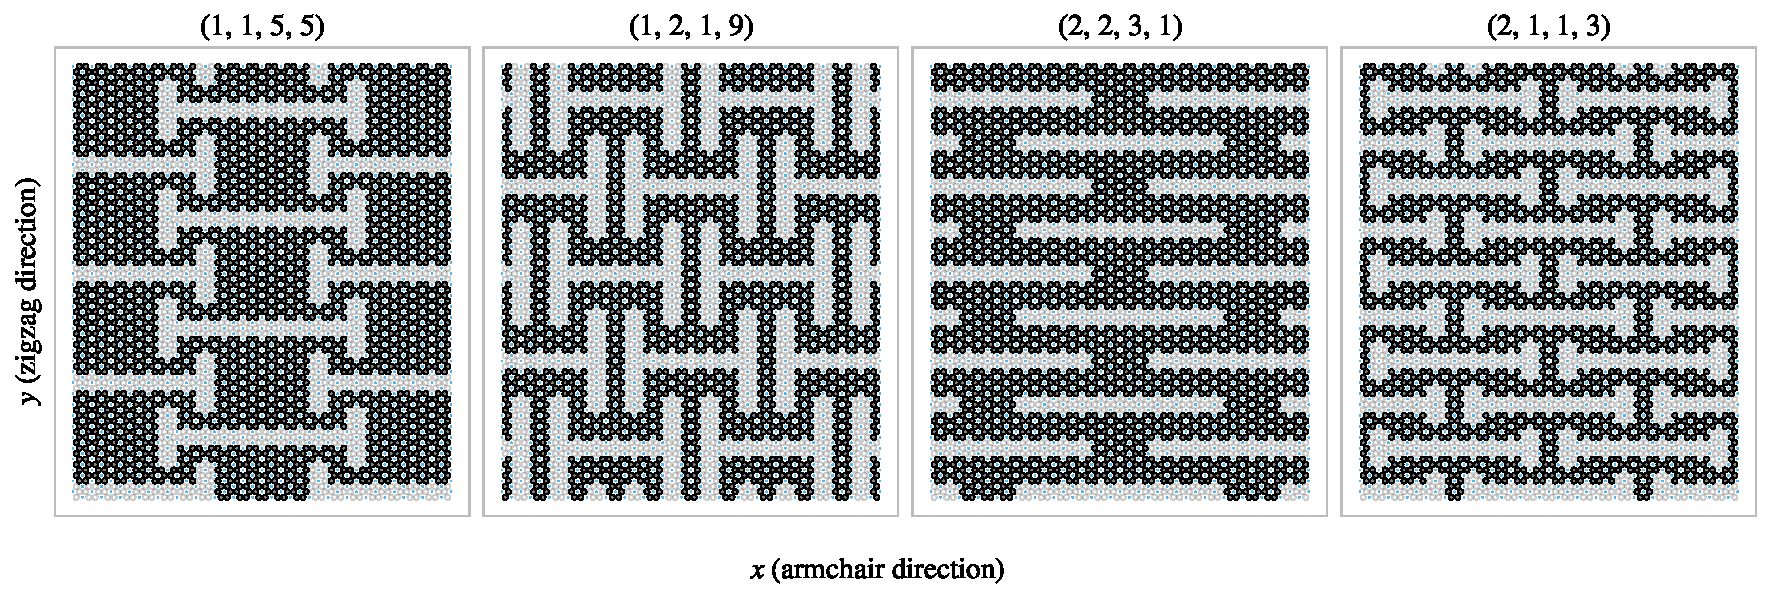
\includegraphics[width=\linewidth]{figures/system/honeycomb_flavors.png}
  \caption{Example of different Honeycomb cut pattern variations. The specific parameters are noted as titles and all of the patterns use the center of the sheet as a reference position. The circles in the figure represent atom sites, where grey-filled circles indicate the presence of atoms and transparent circles indicate removed atoms. The blue dots in the figure indicate the center elements. 
  The sheet matrix size is $40 \times 80$ corresponding to 3200 atom sites and an approximate sheet size of $84 \times \SI{123}{\text{Å}}$.}
  \label{fig:honeycomb_flavors}
\end{figure}



\subsection{Random walk}
The random walk serves as a method for generating Kirigami patterns with randomized features. This approach is motivated by the aim of generating an ensemble of patterns that covers a larger region of the configuration space than the more structured patterns mentioned earlier. This is considered to be important for the quality of the dataset used for machine learning. By this argument, a straightforward way to create random configurations could be achieved simply by random noise, either uniform or Gaussian. However, this would often leave the sheet detached with numerous non-connected atom clusters. Intuitively, we do not find this promising for the generation of large-scale structures which we hypothesize to be of interest. The random walk pattern generation is characterized by the parameters summarized in~\cref{tab:RW_params} which will be introduced throughout the following paragraphs. 

\begin{table}[h]
  \begin{center}
  \caption{Parameters for the random walk generator.}
  \label{tab:RW_params}
  \begin{tabular}{ | c | c | m{8cm} |} \hline
  \textbf{Parameter} & \textbf{Value} & \textbf{Description}  \\ \hline
  Num.\ walkers ($M$) & Integer $\ge$ 1 & Number of random walks to be initiated on the sheet (one at a time). \\ \hline
  Max.\ steps ($S$)  & Integer $\ge$ 1 &The maximum steps allowed for any random walker. \\ \hline
  Min.\ distance  & Integer $\ge$ 0 &The minimum distance required between any future paths and the previous paths in terms of the shortest walking distance in between. \\ \hline
  Bias  & (direction, strength $\ge0$) & Bias direction and strength defining the discrete probability for the choice of the next site. \\ \hline
  Connection  & Atoms / Center elements & Whether to walk between atom sites or center elements removing all adjacent atoms. \\ \hline
  Avoid invalid  & True/False & Whether to remove already visited sites from the neighbor list before picking the next site. This prevents jumping to already visited sites and lowers the likelihood of early termination.  \\ \hline
  Stay or break  & $p = [0,1]$ & Probability that the walker will maintain its direction for the next step. \\ \hline
  Periodic  & True/False & Whether to use periodic boundary conditions on all four sides. \\ \hline
  Avoid clustering  & Integer $\ge$ 0 & Amount of times to restart the whole random walk generation in order to arrive at a non-detached configuration. If no valid configuration is reached after this number of attempts, the non-spanning clusters are removed.\\ \hline
  RN6  & True/False & Randomly change the bias direction between the deployment of each random walker to one of the six center element directions. \\ \hline
  Grid start  & True/False & The option to have the random walkers start in an evenly spaced grid. \\ \hline
  Centering  & True/False & Relocate the path of a random walk after termination such that the path center of mass gets closer to the starting point (without violating the rules regarding already visited sites).\\ \hline
  \end{tabular}
  \end{center}
\end{table}

\subsubsection{Fundamentals} % M, S, Connection, Periodic, Avoid invalid
For an uncut sheet, we deploy $M$ random walkers, one at a time, and let them
walk for a maximum number of $S$ steps. We can either let the walker travel
between atom sites, removing the atoms in the path as it goes, or between the
center elements, removing all surrounding atoms. This is managed by setting the
\textit{connection} parameter to either \textit{atom} or \textit{center
elements}. The method of removing only the intersecting atoms between center
elements was also incorporated, but we ended up not using it due to plenty of
other interesting options. Nonetheless, we will always remove a site once
visited such that the walker itself, or any other walkers, cannot use this site
again. This leads to a self-avoiding random walk, meaning that the walker does
not cross its own path. However, it furthermore constrains the walkers to avoid
the path taken by any previous walker, and thus we might denote this property as
``other avoiding''. By default, the walker has an equal chance of choosing any
of its adjacent neighbors for the next step, i.e.\ we draw the next step from a
discrete uniform distribution. Optionally, we can use periodic boundary
conditions, by setting the parameter \textit{periodic} to true,
allowing neighboring sites to be connected through the edge in both the x and
y-direction. When traveling on atom sites this ensures that we have three
neighbor options for the next step while traveling on the center elements this
gives six neighbor options. If the walker happens to arrive at an already
visited site the walk is terminated early. Optionally, we can choose to remove
any neighboring sites already visited from the neighbor list and choose
uniformly between the remaining options instead. This is done by setting the
parameter \textit{avoid invalid} to true. This prolongs the walking distance,
but the walker is still able to find itself in a situation where no neighboring
sites are available. Note that the walker is not allowed to backtrack its own
path either, and thus in such a case the walk will be terminated despite the
setting of \textit{avoid invalid}.


\subsubsection{Spacing of walking paths} % minimum distance
To control the spacing between the paths of the various walkers, we implement a so-called \textit{minimum distance} parameter, taking integer values $\ge 0$. This parameter describes the minimum spacing required between paths in terms of the least amount of walking steps. When a walker has ended its walk, either by early termination or hitting
the maximum limits of steps, all sites within walking distance corresponding to the minimum distance parameter are marked as visited, although they are not removed from the sheet.
This prevents any subsequent walkers to visit those sites in their walk
according to the general behavior introduced in the previous paragraph. In
practice, this is done through a recursive algorithm as described in~\cref{algo:walk_dis}. For a given path the function \textit{walk\_distance()} is called with the input being a list of all sites in the given paths. The function gathers all the neighbors of each site, regardless of their state on the sheet. It then calls itself recursively using this neighbor list as input, while incrementing a distance counter that is also passed along as an argument. This results in an expansion along all possible outgoing paths from the initial path of interest. Once the distance limit is reached, the function returns the final neighbor lists, which are then accumulated into a final output. This output corresponds to a list of all sites within the minimum distance to the path.


\begin{algorithm}[!htb]
  \caption{Recursive algorithm implemented as a class method of the random walk generator. For a given path input it flags all sites within a distance given by the class attribute \textit{self.min\_dis}.}
  \label{algo:walk_dis}
  \begin{algorithmic}[1]
    \Require self.min\_dis $>$ 0 
    \Function{walk\_distance}{self, input, dis = 0, pre = [ ]}
      \State new\_neigh $\gets$ [ ] \Comment{Initialize list for new neighbors}
      \For{site in input}
        \State neigh $\gets$ get\_neighboring\_sites(site) \Comment{Get surrounding neighbors}
        \For{n in neigh}
          \If {(n not in pre) and (n not in new\_neigh)} \Comment{If not already added}
            \State AddItem(new\_neigh, n) \Comment{then add the site}
          \EndIf
        \EndFor
      \EndFor
      \State dis += 1 \Comment{Increment distance counter}
      \If{dis $\ge$ self.min\_dis} \Comment{Max limit hit}
        \State \Return input + new\_neigh 
      \Else \Comment{Start a new walk from each of the neighboring sites}
        \State pre $\gets$ input
        \State \Return pre +  self.walk\_distance(new\_neigh, dis, pre)
      \EndIf
    \EndFunction
  \end{algorithmic}
\end{algorithm}


\subsubsection{Bias} % Bias
We provide the option to perform a biased random walk by specifying the
\text{bias} parameter, which consists of a direction and a strength. To achieve
this, we model each step of the walk analog to a system in the canonical
ensemble under the influence of an external force $\vec{F}$ representing the
bias. For such a system each microstate $i$, corresponding to the sites in the
neighbor list, has the associated probability $p_i$ given by the Gibbs–Boltzmann
distribution
\begin{align*}
  p_{i} = \frac{1}{Z}e^{-\beta E_i}, \qquad Z = \sum_i e^{-\beta E_i},
\end{align*}
where $Z$ is the canonical partition function, $\beta = 1/k_B T$ for the
boltzmann constant $k_B$ and temperature $T$, and $E_i$ the energy of site $i$.
We model the energy of each site as the work required to move there. For a step
$\vec{s}$ the energy becomes $E_i = -\vec{s}\cdot\vec{F}$, where the sign is chosen such that the energy (difference) is negative when moving along the bias, analogous to an energy gain by
moving there. Due to the symmetry of the random walk sites, both for the atom sites and the center elements, the step length to neighboring sites will always be equal. By defining
the bias strength $B = \beta|\vec{F}||\vec{s}|$ we get that the probability for
jumping to site $i$ is
\begin{align*}
  p_i = \frac{1}{Z}e^{B\hat{\vec{s}}\cdot\hat{\vec{F}}} \propto e^{B\hat{\vec{s}}\cdot\hat{\vec{F}}},
\end{align*}
 where the hat denotes the unit vector. The bias strength $B$ then captures the opposing effects of the magnitude of the external force and the
 temperature of the system since $B\propto |\vec{F}|/T$. We notice that
 $\hat{\vec{s}}\cdot\hat{\vec{F}} = \cos{(\theta)}$ for the angle $\theta$
 between the step and bias direction. This shows that the bias will have the
 biggest positive contribution to the probability when the step direction is fully aligned with the bias
 direction ($\theta = 0$), have no contribution for orthogonal directions
 ($\theta = \pm \pi/2$) and the biggest negative contribution when the directions
 are antiparallel ($\theta = \pi$). The partition function serves as a
 normalization constant. Thus, numerically we can enforce this simply by setting $Z = 1$ at first, calculating $p_i$, and then normalizing the result at the final stage as a
 division by the sum of all $p_i$. In the numerical implementation, we then pick
 the next step by the weighted discrete probability distribution $p_i$. In~\cref{fig:bias_prob} we have illustrated how a bias of different strengths impacts the probability distribution for a random walk between center elements. We can visually confirm that the bias will favor sites that lie close to the bias direction. This preference is more distinct at high bias strengths while at low strength $B\to0$ we get a uniform distribution that aligns with the default unbiased random walk. 

\begin{figure}[!htb]
  \centering
  \begin{subfigure}[t]{0.48\textwidth}
      \centering
      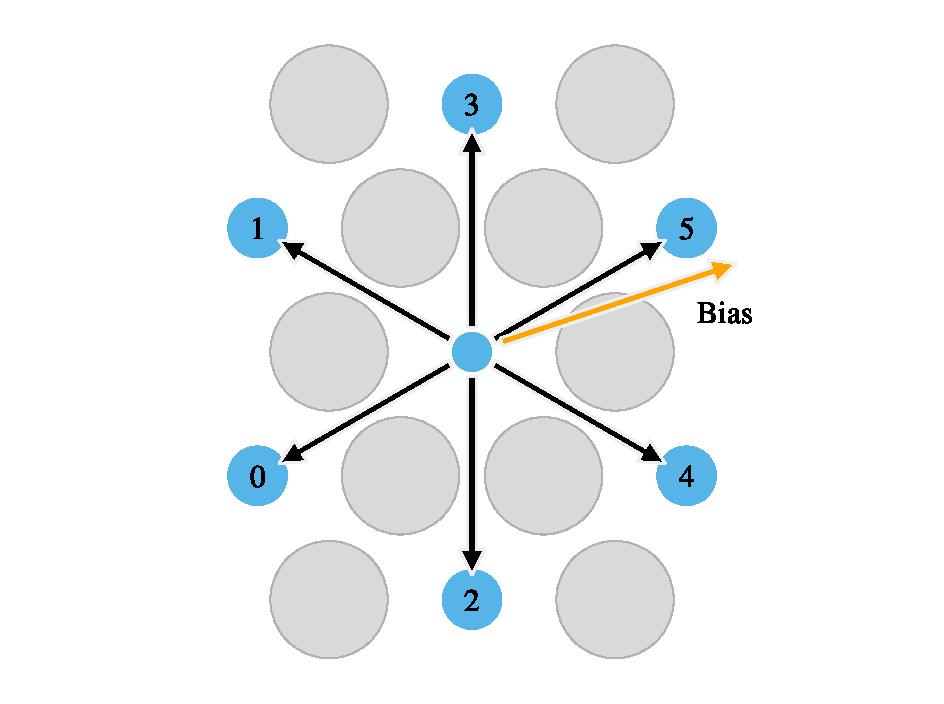
\includegraphics[width=\textwidth]{figures/system/bias_prob_a.pdf}
      \caption{}
      \label{fig:bias_prob_a}
    \end{subfigure}
    \hfill
    \begin{subfigure}[t]{0.48\textwidth}
      \centering
      \includegraphics[width=\textwidth]{figures/system/bias_prob_b.pdf}
      \caption{}
      \label{fig:bias_prob_b}
  \end{subfigure}
  \hfill
     \caption{Illustration of the probability distribution for the various step directions during a biased random walk between center elements. (a) The possible step directions are represented by black arrows that point towards the neighboring center elements depicted as blue circles. The bias direction is denoted by an orange arrow, and the numbering indicates the most probable direction (1) towards the least probable direction (6). The atom sites are marked as grey circles for reference. (b) The probability distribution as a function of the angle $\theta$ between the step direction and the bias direction. The distribution is normalized according to the discrete probabilities marked with dots for which the continuous line simply highlights the shape of the distribution. The direction indexes correspond to the numbering on panel (a). The color map indicates different strengths of the bias. }
     \label{fig:bias_prob}
\end{figure}


\subsubsection{Stay or break}
The \textit{stay or break} parameter defines the probability
$p_{\text{stay}}$ that the walker will keep its direction or otherwise break
into a different direction by probability $1-p_{\text{stay}}$. We implement this by altering the discrete probability used for the choice of the next step. We manually set the probability to $p_{\text{stay}}$ for the site corresponding to a continuation in the same direction and renormalize the distribution. This allows us to perform a biased random walk in combination with a preference for keeping direction. For the center element
walk it is trivial to determine which of the neighbor directions correspond to
a continuation of direction based on the last visited site. However, for an atom site walk, it is not possible to follow the same direction in a straight line due to the hexagonal layout of the lattice. We recall that the
nearest atom neighbor indexes alternate for each increment in the x or y index (see~\cref{eq:atom_neigh_idx}) which corresponds to the alternating neighbor directions $D$ as
\begin{align*}
  (i + j) \ \text{is even} &\rightarrow D = \left\{ \frac{a}{2}\left(\frac{-2}{\sqrt{3}}, 0\right), \frac{a}{2}\left(\frac{1}{\sqrt{3}}, 1\right), \frac{a}{2}\left(\frac{1}{\sqrt{3}}, -1\right)\right\}, \\
  (i + j) \ \text{is odd} &\rightarrow D = \left\{ \frac{a}{2}\left(\frac{2}{\sqrt{3}}, 0\right), \frac{a}{2}\left(\frac{-1}{\sqrt{3}}, 1\right), \frac{a}{2}\left(\frac{-1}{\sqrt{3}}, -1\right)\right\}.
\end{align*}
One way to mitigate this issue is to use the six directions from the center element walk as the common direction to ``stay or break'' from. As showcased in~\cref{fig:stay_or_break}, for each center element direction (black arrows) there are two possible atom site directions (red and orange arrows) that are equally close to the center element direction. The red and orange arrows represent $(i+j)$ being even or odd respectively, and we notice that these appear in pairs such that we can always uniquely determine which of the atom directions is closest to the center element direction. Following this idea we can map each center direction to an atom direction depending on the even or oddness of the position. For $p_{\text{stay}} = 1$ this results in a guaranteed zigzag motion along the center element direction that it happens to start on. 

\begin{figure}[!htb]
  \centering
  \includegraphics[width=0.5\linewidth]{figures/system/stay_or_break.pdf}
  \caption{Visualization of the center element directions (black arrows) connecting the center elements depicted as blue dots, and the atom site directions (red and orange arrows) connection the atom sites depicted as grey circles. The red arrows correspond to the case where the sum of the atom site indexes $(i,j)$ is even, while the orange arrows correspond to the case where the sum is odd. Notably, for each case, there is always one atom site direction that is uniquely closest to a given center element direction.}
  \label{fig:stay_or_break}
\end{figure}

The \textit{stay or break} feature is still subject to previously defined rules.
For instance, in the case where the preferred site is not available, the walker
will either terminate when going there, or the preferred site is removed from
the neighbor list when \textit{avoid invalid} is set to true. In the latter
case, the walker will be forced to break out of its direction and follow the new
direction that it happens to choose.


\subsubsection{Deployment schemes} % Grid start, Centering, RN6
By default, each random walker is given a uniform random starting point among
the non-visited available sites left on the sheet. This includes any
modifications in relation to the minimum distance parameter. By setting the
\textit{grid start} parameter to true, the starting points are instead
predefined on an evenly spaced grid. That is, the sheet is subdivided into the
least amount of squares that will accommodate space for each starting point. $\{1\}$
walker leads to a $1\times 1$ partition, $\{2,3,4\}$ walkers lead to a $2\times
2$ partition, $\{5,6,7,8,9\}$ walker lead to a $3\times 3$ partition and so on.
For each partition square, the starting point is placed as centrally as
possible. The lower left partition square is then chosen as a default starting
place for the first walker and the remaining sites are filled according to the
order that maximizes the minimum distance between a new starting point and the
ones already occupied\footnote{In hindsight, we realize that it would have been less biased to
choose a random partition square as the starting one, but we do not consider
this to be of great importance for the usage of this feature in the dataset.}.
An example of the deployment is shown in~\cref{fig:grid_start}. Notice, that if the planned grid start position is made invalid before deployment, it is skipped. 


\begin{figure}[!htb]
  \centering
  \includegraphics[width=0.90\linewidth]{figures/system/grid_start.pdf}
  \caption{The figure illustrates the distribution of starting points when the \textit{grid start} parameter is set to true for a $14\times 18$ sheet, for varying numbers of deployed random walkers ranging from 1 to 9. The color map is used to indicate the order in which the walkers were deployed.}
  \label{fig:grid_start}
\end{figure}

The \textit{centering} parameter lets us relocate the path of the random walker
such that the path center of mass gets closer to the starting point. When set to true, the path is moved in the direction defined from the center of mass toward 
the starting point for which the closest valid relocation on the direct
translation line is chosen. This can be used in combination with the
\textit{grid start} and the \textit{bias parameter} to make rather ordered
configurations. In addition, the \textit{RN6} parameter can be used to update
the bias direction to one of the six center element directions for each new
walker deployed. This lets us create more organized configurations like the one shown
in~\cref{fig:RW_flavors}\textcolor{red!50!black}{b}. 


\subsubsection{Validity}
The simulation procedure requires the sheet to be fully attached, non ruptured, which can be summarized as the following requirements. 
\begin{enumerate}
  \item There exists only a single cluster on the sheet. We define a cluster as the set of atoms which can all be reached through nearest neighbor walking on the cluster.
  \item The cluster of atoms is spanning the sheet in the y-direction. This means that there exists at least one path through nearest neighbor walking that connects the bottom and the top of the sheet. This is required because the sheet must be attached to the pull blocks in the simulation.
\end{enumerate}
In order to accommodate these requirements we count the number of clusters and search for a spanning cluster after all walkers have terminated. If the requirements are not met we simply rerun the random walk from scratch. This is done according to the \textit{avoid clustering} parameter which takes integer values corresponding to the number of times to repeat this process. If the requirements are not met during any of those reruns the non-spanning clusters are simply removed. In the case of no spanning cluster, the configuration is skipped. This crude scheme was later reinvented as a more refined repair scheme that alters the sheet with the intention of performing the least amount of changes, addition or subtraction of atoms, in order to meet the attachment requirements. This was done as a part of the accelerated search procedure and hence it was not utilized in the creation of the random walk dataset. However, we give a brief description of the algorithm here:
\begin{enumerate}
  \item Find all clusters and rank them in descending order of size, such that the largest cluster is labeled as cluster 1.
  \item Deploy walkers from the edges of the smallest cluster, allowing them to walk in all possible directions similar to what was done with~\cref{algo:walk_dis}. Here the allowed walking distance is defined as the number of atoms within the starting cluster.
  \item If a walker from the starting cluster reaches another cluster within the allowed walking distance, these two clusters are connected through the walking path. Otherwise, the starting cluster is deleted. This decision is based on the consideration that the number of atoms required to connect the clusters should not exceed the number of atoms removed if the starting cluster is deleted. However, if the starting cluster is the last cluster connected to the top or bottom edge, an unlimited number of walks are allowed to ensure the creation of a spanning cluster.
  \item If there is only one cluster remaining on the sheet, the repair procedure is complete. If there are still multiple clusters, then repeat the steps from 1. Note, that if no spanning cluster was ever present, we expand the final cluster until a spanning connection can be established.
\end{enumerate}  
\subsubsection{Random walk examples}
Some examples of the random walk patterns are illustrated in~\cref{fig:RW_flavors} with corresponding parameters in~\cref{tab:RW_flavors}.

\begin{figure}[!htb]
  \centering
  \includegraphics[width=1\linewidth]{figures/system/RW_flavors.png}
  \caption{Example of different Random walk cut pattern variations. The specific parameters are given in~\cref{tab:RW_flavors}. The circles in the figure represent atom sites, where grey-filled circles indicate the presence of atoms and transparent circles indicate removed atoms. The sheet matrix size is $62 \times 106$ corresponding to the full-size system used in the \acrshort{MD} simulations with 6572 atom sites and an approximate sheet size of $130 \times \SI{163}{\text{Å}}$.}
  \label{fig:RW_flavors}
\end{figure}

\begin{table}[h]
  \begin{center}
  \caption{Parameters for the random walk patterns shown in~\cref{fig:RW_flavors}.}
  \label{tab:RW_flavors}
  \begin{tabular}{ |c|M{2.2cm}|M{2.2cm}|c|c|M{2.2cm}|M{2.2cm}|} \hline
  Fig.\ num. & (a) & (b) & (c) & (d) & (e) & (f) \\ \hline 
  Num.\ walkers & 25 & 25 & 20 & 30 & 20 & 32 \\ \hline 
  Max.\ Steps & 15 & 15 & 30 & 40 & 30 & 30 \\ \hline 
  Min.\ distance & 0 & 0 & 4 & 4 & 4 & 4 \\ \hline 
  Bias & $\begin{pmatrix} \text{upper right} \\ 100 \end{pmatrix}$ & $\begin{pmatrix} \text{upper right} \\ 100 \end{pmatrix}$ & None & None & $\begin{pmatrix} \text{lower right} \\ 1.2 \end{pmatrix}$ & $\begin{pmatrix} \text{lower left} \\ 1.2 \end{pmatrix}$ \\ \hline 
  Connection & Atoms & Atoms & Atoms & Atoms & Atoms & Center elements \\ \hline  
  Avoid invalid & False & False & True & True & True & True \\ \hline  
  Stay or break & 0 & 0 & 0.9 & 0 & 0 & 0 \\ \hline  
  Periodic & True & True & True & True & True & True \\ \hline  
  Avoid clustering & 10 & 10 & 10 & 10 & 10 & 10 \\ \hline  
  RN6 & False & True & True & False & False & False \\ \hline 
  Grid start & True & True & False & False & False & False \\ \hline 
  Centering & True & True & False & False & False & False \\ \hline 
  \end{tabular}
\end{center}
\end{table}


 % Chapter 5
% % TO-DO: Look at friction force graph again and reconsider whether we have stick-slip. The small oscillations is perhaps noise, and since the big oscialltions go by smooth curves this is actually more likely to be smooth sliding. I guess looking at the period in connection with the lattice spacing show whether it is thoose curves we should look at or the smaller ones result from a lot of small slips...

% Note: A good word for the force curves is "Force traces" as used by \cite{Yalin_2011}.


\chapter{Pilot study}
Having defined our system, we carry out an initial study of the numerical approach. This includes an analysis of how to define and measure the frictional properties of interest, and an investigation of the main parameters governing the numerical solutions. From this point of view we decide on suitable parameters for the remaining study. Particually, we investigate the frictional behaviour under the variation of load and stretch for a selected set of configurations which serves as a baseline for later comparison and an assessment of the prospects of Kirigami modifications for friction. 


\section{Friction simulation parameters}
The \acrshort{MD} simulation is governed by a small set of parameters, some
which are related directly to the numerical aspects of the simulation and other related
to the physical conditions we are simmulating. Thus, we differentiate between
the two main categories: 1) \textit{Physical}, parameters which alter the
physical conditions of the ``numerical experiment'' and are expected to effect
the frictional behaviour. 2) \textit{Numerical}, parameters which are related
more closely to the numerical procedure itself, expected to influence the
simulation dynamics, which should be chosen to ensure the most stable results.
For the purpose of creating the machine learning dataset most of these
parameters will be kept constant with only a subset of the physical parameters
being varied. The parameters are summarized in \cref{tab:param} where the grey
shaded area marks the parameters, Configuration, stretch and load, which we will vary for the dataset. Due to the great number of parameters it is unreasonable to make an exhaustive search of all parameters before deciding on the final settings. Instead, we take a basis in the parameters used in similar studies \hl{SOURCES} and adjust them as
we carry out the initial analysis of the simulation results. Thus, we start at values
most representative for other similar simulations and adjust according to the
stability of the results and the computation time. Since we are going to
introduce a lot of complexity to the system, through the cut and stretch
deformation, we are less concerned about aligning parameters for comparison. Instead of presenting the process of narrowing down the final parameters in a chronological manner, wehave shown the final choice shown in \cref{tab:param} which we will discuss throughout the following presentation of the pilot study. Notice, that the values in \cref{tab:param} serves as default values which are used when nothing else is stated.



% Thus, by adjusting a few selected parameters one by one we arrived at a final choice as shown in \cref{tab:param}. 

% We will present an analysis of the simulation results and its dependency of these selected variables in the following using the final choice as default values. Thus we should stress that the intention behind this choice is mainly to get a working simulation with stable results and not to optimize for any spefic properties yet. 

% \hl{Say a bit more about the articles used to set a starting reference for these parameters.}

% we proposed a set of parameters for which we investgated the dependencies of only selected ones. By adjusting the parameters according to the findings we landed on a final set as already shown in \cref{tab:param}


% In the following we present the results of the friction simulations in parallel to the procedure of investigating the choice of different parameters. 

% We aim to chose the parameters in order to accomodate a balance between generlizable and stable result which is simmutaneously a suting candidate as a proof of concept for the control of friction properties using kirigami inspired cuts. 



% Due to the great number of parameters, and corresponding range of reasonable numerical values they can take, it is ... to parameter search including all of these. Thus, we will to a great extent rely on a reverse engineering in order to establish a set of parameters for the \textit{physical} and \textit{measurement} categories along with numerical ranges for the $\textit{ML input}$ category which gives stable and promising results. By doing so we effectively narrow down the parameter regime for which the investigated frictional properties belong. We aim to chose the parameters in order to accomodate a balance between generlizable and stable result which is simmutaneously a suting candidate as a proof of concept for the control of friction properties using kirigami inspired cuts. 

% In the following we present the results of the friction simulations in parallel to the procedure of investigating the choice of different parameters. 

% In the following subsections (X to Y) we are going to present the friction simulation results in parallel to the presentation of the reasoning behind the parameter choices. For this we will refer to the default parameter choice showcased in \cref{tab:final_param} which is representative of the final parameter choices. 




% The sliding velocity is 20 m/s, which is comparable to the operating conditions in micromechanical systems (MEMS), but which is much larger than the typical velocity in scanning force microscopy (SFM) experiments. \cite{mo_friction_2009} Supplementary materials.


% We should try to set the physcis and measurement parameters in such a way that we reduce computation speed where it is doesn't infer with the frictional properties study.

\begin{table}[H]
  \begin{center}
  \caption{Parameters of the numerical \acrshort{MD} simulation for measuring friction. The values correspond to the final choice used for the dataset. The shaded area denote the parameters varied in the \acrshort{ML} dataset.}
  \label{tab:param}
  \begin{tabular}{ | c | C{3cm} | C{3.5cm} | X{7cm}|} \hline
    Category & Parameter & Value &  Description \\ \hline
    \multirow{13}{*}{Physical} & $T$ & \SI{300}{K} &  Temperature. \\ \hhline{~|-|-|-|}
    & $v_{\text{slide}}$ &\SI{20}{m/s} & Sliding speed for the sheet translation. \\ \hhline{~|-|-|-|}
    & $K$ & $\inf$ & Spring constant for the coupling between the virtuel atom and the sheet pull blocks. \\ \hhline{~|-|-|-|}
    & Scan direction & $(x,y) = (0,1)$ \linebreak (zigzag direction)  & The direction for which we translate the sheet. \\ \hhline{~|-|-|-|}   
    & \cellcolor{black!7} Sheet configuration & \cellcolor{black!7} Contiguous & \cellcolor{black!7} Binary mapping describing which atoms are removed (0) and which is still present (1) in the graphene sheet.  \\ \hhline{~|-|-|-|}
    & \cellcolor{black!7} Stretch amount & \cellcolor{black!7} 0\% - rupture & \cellcolor{black!7} The relative stretch of the sheet. \\ \hhline{~|-|-|-|}
    & \cellcolor{black!7} $F_N$ & \cellcolor{black!7} [0.1, 10] nN & \cellcolor{black!7} Applied normal force to the pull blocks. \\ \hline
    \multirow{8}{*}{Numerical} & $dt$ & \SI{1}{fs} &  Integration timestep. \\ \hhline{~|-|-|-|}
    & $t_R$ &  \SI{15}{ps} & Relaxtion time before strething. \\ \hhline{~|-|-|-|}
    & Pauses & \SI{5}{ps} & Relaxtion pauses after stretch, and during the normal load phase (before translating the sheet). \\ \hhline{~|-|-|-|}
    & Stretch Speed & \SI{0.01}{ps^{-1}} & The rate of stretching for the sheet. \\ \hhline{~|-|-|-|}
    & Slide distance & \SI{400}{Å} & How far to translate the sheet. \\ \hhline{~|-|-|-|}
    & Sheet size & $130.029 \times \SI{163.219}{\text{Å}}$ & Spatial 2D size of the sheet.  \\ \hhline{~|-|-|-|}
    & Pull block size & $2 \times 130.029 \times \SI{15.183}{\text{Å}}$ & Spatial 2D size of the pull blocks. \\ \hline
  \end{tabular}
  \end{center}
\end{table}



% Parameters expected to have a physical effect on the friction properties, which is kept fixed and thus not included in the machine learning input set. 

% Paramters influecing the simulation kinetics and being representative of the experimental procedure that we are mimicking. These parameters is chosen with the aim of getting stable parameters under small perturbations of the given parameter. 

% The remaining paramters serves as input variables for optimization process and is thus given as input variables for the machine learning (ML).




% Say someting about how these parameters is chosen. Reference to articles for which these was mirrored from. 





% We need to define some ranges for the ML input paramters. $F_N$, stretch ranges where it is not prone to ruptures. The configuration it self does not have clear rules but is also being regulated by the no rupture requirement. 

% Retardation effects due to the finiteness of the speed of sound are usually irrelevant in slow-speed experiments (v < 1 mm/s) \cite{Manini_2016}

% In macroscopic tribology experiments, sliding speeds often range in the 0.1 − 10 m/s region \cite{Manini_2016}

% By contrast, in nanoscale AFM experiments the tip usually advances at much lower speeds $\sim$ 1 $\mu$m/s: over a typical run it is possible to simulate a tiny ∼ 1 pm displacement, far too small to explore even a single atomic-scale event, let alone averaging over a steady state.\cite{Manini_2016}


% However, MD simulations can provide so much physical insight that they make sense even if carried out at much higher speeds than in real-life AFM or surface force apparatus (SFA) experiments: in practice, currently the sliding speeds of most atomistic tribology simulations are in the $\sim$ 1 m/s region.\cite{Manini_2016}


% Besides the limitations of system size and simulation times that are obvious and will be discussed later, there is another limitation concerning temperature, that is rarely mentioned. All classical frictional simulations, atomistic or otherwise, are only valid at sufficiently high temperature. They become in principle invalid at low temperatures where the mechanical degrees of freedom of solids progressively undergo ”quantum freezing”, and both mechanics and thermokinetics deviate from classical. \cite{Manini_2016}.




% \newpage
% Single friction simulation analysis
\section{Force traces}\label{sec:single_analysis}
We begin by assessing the friction force traces, i.e.\ force vs.\ time curves, for a single friction simulation using the default parameters shown in \cref{tab:final_param} for a non-cut sheet with
no stretch applied and a normal load of $\SI{1}{nN}$. 


\subsection{Force oscillations}\label{sec:force_oscillations}
We evaluate the friction force as the force acting on the sheet from the
substrate. We consider initially the force componenet $F_{\parallel}$ parallel
to the drag direction as plotted in \cref{fig:drag_Ff}. We use a sample rate of
10 ps$^{-1}$ = 100 timesteps$^{-1}$ for which each sample is the mean value of
the preceding 100 timesteps. We observe immediately that the data carriers
oscillations on different time scales matching our general expectations for
sliding involving periodic surfaces. By applying a savgol filter to the data
with a polyorder of 5 and window length of 150 timesteps (corresponding to a
sliding distance of 3 Å or a time window of 15 ps) we can qualitatively point
out at least two different frequencies of osccilation. During the first 10 Å of
sliding, seen in \cref{fig:drag_Ff_10}, we see roughly three waves on the savgol
filter corresponding to a relative high frequency, while for the duraction of
100 Å of sliding, seen in \cref{fig:drag_Ff_100}, the same savgol filter reveals
a lower frequency on top, creating the visual pattern of a wavepacket. The data
does not indicate clear signs of stick-slip behaviour as otherwise found in
other studies, e.g.\ by Zhu and Li \cite{zhu_study_2018} for graphene on gold,
who saw a more typical saw tooth shape in the force trace. Beside the difference
in substrate material, using gold instead of silicon, they used a lower sliding
speed of \SI{10}{m/s} and a soft spring of $K = \SI{10}{N/m}$. By adopting those
parameters we get a slightly different force trace behaviour as shown in
\cref{fig:drag_Ff_10_K10_v10} and \cref{fig:drag_Ff_100_K10_v10}. This change
breaks the symmetry in the force oscillations, but still does not produce any
significant discontinuities in the trace. By keeping the spring constant $K =
\SI{10}{N/m}$ and lowering the sliding speed further down to \SI{1}{m/s} we are
able to demonstrate a proper stick-slip behaviour as shown in
\cref{fig:drag_Ff_10_K10_v1} and \cref{fig:drag_Ff_100_K10_v1}. Considering all
three simulations we might classify the results from the default settings, $K =
\inf, v = \SI{20}{m/s}$, as smooth sliding,  $K = \SI{10}{N/m}, v =
\SI{10}{m/s}$, as a transistion phase with possible occasional slipping, and $K
= \SI{10}{N/m}, v = \SI{1}{m/s}$ as certain stick-slip behaviour.

\hl{Refer a bit to theory on this one}

%  This result agrees with ... that the stick-slip
% behaviour is suppresed for high sliding speed and stiff springs. 

However, the low sliding speed comes with a high computational cost which is the reason that we choose a sliding speed of \SI{20}{m/s}. The choise of an infinite spring constant is related to the stability of the measurements as discussed later \hl{make reference}.


\begin{figure}[H]
  \centering
  \begin{subfigure}[t]{0.49\textwidth}
      \centering
      \includegraphics[width=\textwidth]{figures/baseline/drag_Ff_10Å.pdf}
      \caption{$K = \inf$, $v = \SI{20}{\frac{m}{s}}$ (10 Å sliding).}
      \label{fig:drag_Ff_10}
  \end{subfigure}
  \hfill
  \begin{subfigure}[t]{0.49\textwidth}
      \centering
      \includegraphics[width=\textwidth]{figures/baseline/drag_Ff_100Å.pdf}
      \caption{$K = \inf$, $v = \SI{20}{\frac{m}{s}}$ (100 Å sliding).}
      \label{fig:drag_Ff_100}
    \end{subfigure}
    \hfill
    \begin{subfigure}[t]{0.49\textwidth}
      \centering
      \includegraphics[width=\textwidth]{figures/baseline/drag_Ff_10Å_K10_v10.pdf}
      \caption{$K = \SI{10}{\frac{N}{m}}$, $v = \SI{10}{\frac{m}{s}}$ (10 Å sliding).}
      \label{fig:drag_Ff_10_K10_v10}
    \end{subfigure}
    \hfill
    \begin{subfigure}[t]{0.49\textwidth}
      \centering
      \includegraphics[width=\textwidth]{figures/baseline/drag_Ff_100Å_K10_v10.pdf}
      \caption{$K = \SI{10}{\frac{N}{m}}$, $v = \SI{10}{\frac{m}{s}}$ (100 Å sliding).}
      \label{fig:drag_Ff_100_K10_v10}
  \end{subfigure}
  \hfill
    \begin{subfigure}[t]{0.49\textwidth}
      \centering
      \includegraphics[width=\textwidth]{figures/baseline/drag_Ff_10Å_K10_v1.pdf}
      \caption{$K = \SI{10}{\frac{N}{m}}$, $v = \SI{1}{\frac{m}{s}}$ (10 Å sliding).}
      \label{fig:drag_Ff_10_K10_v1}
    \end{subfigure}
    \hfill
    \begin{subfigure}[t]{0.49\textwidth}
      \centering
      \includegraphics[width=\textwidth]{figures/baseline/drag_Ff_100Å_K10_v1.pdf}
      \caption{$K = \SI{10}{\frac{N}{m}}$, $v = \SI{1}{\frac{m}{s}}$ (100 Å sliding).}
      \label{fig:drag_Ff_100_K10_v1}
  \end{subfigure}
  \hfill
     \caption{Force traces of the friction force $F_\parallel$ with respect to the drag direction between acting from the substrate on the full sheet and substrate. The force traces is plotted against the sliding distance (lower x-axis) and thr corresponding sliding time (upper x-axis). The sliding distance is measured by displacement of the virtual atom tethering the sheet. The red line represents a savgol filter with window polyorder 5 and window length of 150 timesteps (corresponding to a sliding distance of 3 Å or a time window of 15 ps). Each row, (a,b), (c,d), (e,f), represents a different choice of the spring constant $K$ and sliding speed $v$, while the columns show the same result for two different time scales. The default settings are represented in figure (a) and (b).}
     \label{fig:drag_Ff}
\end{figure}

By performing a Fourier Transform on the data, using the default parameters, we can quantify the leading frequencies observed in figure \cref{fig:drag_Ff_10} and \cref{fig:drag_Ff_100}. The Fourier transform is shown in \cref{fig:ft_a}, and by plotting the two most dominant frequencies $f_1 = 0.0074$ ps$^{-1}$ and $f_2 = 0.0079$ ps$^{-1}$ as a sine sum, $\sin{(2\pi f_1)} + \sin{(2\pi f_2)}$, we find a qualitatively convincing fit to the observed wavepacket shape as seen in \cref{fig:ft_b}. We can convert the frequencies according to that of a wavepacket. By using the trigonometric identity
\begin{align*}
\sin (a+b) &= \sin (a) \cos (b) + \cos (a) \sin (b), \\
\sin (a-b) &= \sin (a) \cos (b) - \cos (a) \sin (b),
\end{align*}
and decomposing the frequencies as $f_1 = a - b$, $f_2 = a + b$, we can rewrite the sine sum as the sinusoidal product
\begin{align*}
  \sin(2\pi f_1) + \sin(2\pi f_2) &= \sin\big(2\pi (a - b)\big) + \sin\big(2\pi (a + b)\big) \\
  &= \sin(2\pi a)\cos(2\pi b) + \cancel{\cos(2\pi a)\sin(2\pi b)} + \sin(2\pi a)\cos(2\pi b) - \cancel{\cos(2\pi a)\sin(2\pi b)} \\
  &= 2 \sin(2\pi a) \cos(2\pi b),
\end{align*} 
with 
\begin{align*}
  a = \frac{f_1 + f_2}{2} &= 0.0763 \pm \SI{0.0005}{ps^{-1}},& 
  b = \frac{f_2 - f_1}{2} &= 0.0028 \pm \SI{0.0005}{ps^{-1}},& \\
  &= 0.381 \pm \SI{0.003}{{\text{Å}}^{-1}},& 
  &= 0.014 \pm \SI{0.003}{{\text{Å}}^{-1}},& 
\end{align*}
where the latter frequency is denoted with respect to the sliding distance. This
makes us recognize the high osccilation frequency as $a$ and the low frequency
as $b$. The faster one has a period of $T_a = 2.62 \pm 0.02$ Å\footnote{The
uncertainty $\Delta y$ is calculated as $\Delta y = \left|\frac{\partial
y}{\partial x} \Delta x \right|$ for uncertainty $\Delta x$ and $y(x)$} which
corresponds well with the magnitude of the lattice spacing and especialy that of
graphene at 2.46 Å as expected theoretically. The longer period $T_b = 71 \pm
15$ Å$^{-1}$ is not obviously explained. We noticed a similar long period osciallation for all three cases, \cref{fig:drag_Ff_100}, \cref{fig:drag_Ff_100_K10_v10} and \cref{fig:drag_Ff_100_K10_v1}, regarding stick-slip behaviour, and thus we not believe that this is directly related. The initial build up in friction force is reminiscent of a friction strengthening, which is often reported \hl{SOURCE}, but the periodicity goes against this idea. Instead, we might attribute it to some kind of phonon
resosnance which could be a physical phenonama or simply a feature of our
\acrshort{MD} modelling. 

\begin{figure}[H]
  \centering
  \begin{subfigure}[t]{0.49\textwidth}
    \centering
    \includegraphics[width=\textwidth]{figures/baseline/ft_zoom.pdf}
    \caption{FT result shown for a reduced frequency range.}
    \label{fig:ft_a}
  \end{subfigure}
  \hfill
  \begin{subfigure}[t]{0.49\textwidth}
      \centering
      \includegraphics[width=\textwidth]{figures/baseline/ft_sine.pdf}
      \caption{Two most dominant frequencies applied to the data from \cref{fig:drag_Ff_100}}
      \label{fig:ft_b}
  \end{subfigure}
  \caption{Fourier transform analysis of the full friction force data (all 400 Å sliding distance) shown in \cref{fig:drag_Ff}. (a) shows the two most dominant frequency peaks. Note that no significant peaks was found in a higher frequency than included here. (b) shows a comparison between the raw data and the wavefunction corresponding to the two peaks in figure (a).}
  \label{fig:ft}
\end{figure}


\subsection{Decompositions}
In the previous analysis we have looked only at the friction force for the full
sheet, including the rigid pull blocks, and with
respect to the drag direction. We found this way of measuring the friction force to be the most intuitive and reliable, but we will present the underlying arguments for this choice in the following.

Due to the fact that we are only applying cuts to the inner sheet, and not the
pull blocks, it might seem more natural to only consider the friction on that
part. If the desired frictional properties can be achieved by altering the inner
sheet one can argue that any opposing effects from the pull blocks can be
mitigated by simply scaling the relative size between the inner sheet and the pull
blocks. However, when looking at the force traces decomposed with respect to the
inner sheet and pull block regions respectivly, see \cref{fig:decomp_group}, we
observe that the friction force arrising from those parts are seemingly
antisymmetric. That is, the distribution of the fricitonal pull from the
substrate on the sheet is oscillating between the inner sheet and the pull
block. Keeping in mind that normal force is only applied to the pull blocks we
might take this as an intrinsic feature of the system which does not nessecary dissapear by scaling of the spatial ratio between the inner sheet and pull block. Any interesting friciton properties might depend on this internal distribution of forces. Hence, we hedge our bets and use the full sheet friction force as a hollistic approach to avoid excluding relevant information in the measurement data.

Similar we might question the decision of
only considering the frictional force projected onto the sliding direction as
we are then neglecting the ``side shift'' induced during sliding. In \cref{fig:decomp_direc} we show the decomposition in terms of force components parallel $F_{\parallel}$ and perpendicular $F_{\perp}$ to the sliding direction respectively. We notice that the most dominant trend appears for the parallel component. If we want to include the perpendicular component as well we would have to evaluate friction as the length of the force vector instead, but this would remove the sign of the force direction and shift the mean friction force up as we clearly see both negative and positive contributions in the parallel force trace. One option to accommodate this issue is by using the vector length for the magnitude but keeping the sign from the parallel component. However, we omit such compromises as this might make the measurement interpretation unessercary complex, and we use only the parallel component going forward. 

\begin{figure}[H]
  \centering
  \begin{subfigure}[t]{0.49\textwidth}
    \centering
    \includegraphics[width=\textwidth]{figures/baseline/decomp_group.pdf}
    \caption{}
    \label{fig:decomp_group}
  \end{subfigure}
  \hfill
  \begin{subfigure}[t]{0.49\textwidth}
      \centering
      \includegraphics[width=\textwidth]{figures/baseline/decomp_direc.pdf}
      \caption{}
      \label{fig:decomp_direc}
  \end{subfigure}
  \caption{Friction force decomposition on the default parameter force trace shown in \cref{fig:drag_Ff} showing only the applied savgol filters. (a) Decomposition into group inner sheet (sheet) and pull blocks (PB). (b) Decomposition into parallel ($F_{\parallel}$) and perpendicular ($F_{\perp})$ to drag sliding direction.}
  \label{fig:decomp}
\end{figure}


\subsection{Center of mass path}
From the previous observations of the force traces \cref{fig:drag_Ff} we
demonstarted both smooth sliding and stick-slip behaviour. Considering the force
decomposition in \cref{fig:decomp_direc} we know that the frictional forces in
the perpendicular direction to sliding is also present. By looking at the
$x,y$-position for the sheet Center of Mass (\acrshort{CM}) we see a qualitative
different behaviour when reconsidering the spring constant and sliding speed
investigated in \cref{fig:drag_Ff} which is shown in \cref{fig:CM_path}. The
default case in \cref{fig:CM_path_def} shows a rather straight path forward with
only a small side motion in comparison to the cases in
\cref{fig:CM_path_K10_v10} and \cref{fig:CM_path_K10_v1}. However, the
\acrshort{CM} accelerates and deaccelerates with a high frequency, much to high
to be associated with the lattice spaing on the order of 2.46 Å (interatomic
distance of 1.42 Å). One possible explanation is that the sheet and substrate
constitues an incommensurable contact for which travelling kink excitations make
the atoms move in such a way that the sheet \acrshort{CM} is incremented in
small ``burst''. When looking at the $K = \SI{10}{\frac{N}{m}}$, $v =
\SI{10}{\frac{m}{s}}$ case in \cref{fig:CM_path_K10_v10} we see a completely
different \acrshort{CM} path where the rapid parts alligns visually better with
the force oscialltiosn shown earlier in \cref{fig:drag_Ff_100_K10_v10}. The
\acrshort{CM} accelerates forward and the deaccelerates in combination with a
side motion that lead to the \acrshort{CM} path making a loop as it slows down.
Finally we have the $K = \SI{10}{\frac{N}{m}}$, $v = \SI{10}{\frac{m}{s}}$ in
\cref{fig:CM_path_K10_v10} which is confirmed to have stick-slip behaviour in
\cref{fig:drag_Ff_100_K10_v1}. Here the \acrshort{CM} path shows a more chaotic
movement between acceleration which also alligns visually well with the timing
of the slips seen in \cref{fig:drag_Ff_100_K10_v1}. The chaotic motion is not
obviously connected to the stick-slip motion, but we ommit a further
investigation as this is not corresponding to the parameters that we will be
using. 


\begin{figure}[H]
  \centering
  \begin{subfigure}[t]{0.85\textwidth}
    \centering
    \includegraphics[width=\textwidth]{figures/baseline/COM_path_K0.pdf}
    \caption{$K = \inf$, $v = \SI{20}{\frac{m}{s}}$.}
    \label{fig:CM_path_def}
  \end{subfigure}
  \hfill
  \begin{subfigure}[t]{0.85\textwidth}
    \centering
    \includegraphics[width=\textwidth]{figures/baseline/COM_path_K10_v10.pdf}
    \caption{$K = \SI{10}{\frac{N}{m}}$, $v = \SI{10}{\frac{m}{s}}$.}
    \label{fig:CM_path_K10_v10}
  \end{subfigure}
  \begin{subfigure}[t]{0.85\textwidth}
    \centering
    \includegraphics[width=\textwidth]{figures/baseline/COM_path_K10_v1.pdf}
    \caption{$K = \SI{10}{\frac{N}{m}}$, $v = \SI{1}{\frac{m}{s}}$.}
    \label{fig:CM_path_K10_v1}
  \end{subfigure}
  \caption{Center of Mass (\acrshort{CM}) position relative to the start of the sliding phase in terms of the direction parallel to the sliding direction $\Delta COM_{\parallel}$ and the axis perpendicular to the sliding direction $\Delta COM_{\perp}$. The colorbar denotes the absolute speed of the \acrshort{CM} motion. Figure a-c shows different parameters used for the spring constant $K$ and sliding speed $v$ similar to that used in \cref{fig:drag_Ff}. (a) Default: $K = \inf$, $v = \SI{20}{\frac{m}{s}}$. (b) $K = \SI{10}{\frac{N}{m}}$, $v = \SI{10}{\frac{m}{s}}$. (c) $K = \SI{10}{\frac{N}{m}}$, $v = \SI{1}{\frac{m}{s}}$ }
  \label{fig:CM_path}
\end{figure}


\section{Defining metrics for friction}\label{sec:def_dyn_and_stat}

In order to evaluate the frictional properties of the sheet we aim to reduce the force trace results, adressed in section \cref{sec:single_analysis}, into single metrics describing the kinetic and static friciton resepctively. 

\subsection{Kinetic friction} 
We measure kinetic friction as the mean of the friction force trace. More
precisly, we take the mean value of the latter half of the dataset in order to
ensure that we are sampling from a stable system. For a full sliding simulation
of 400 Å we thus base our mean value on the latter 200 Å (1000 ps) of sliding.
In \cref{fig:runmean} we have shown the force trace for the first 10 Å of
sliding together with a 50\% running mean window. The choice of such a short sliding distance is merely to illustrate the samplig procedure,
and we see that the final mean estimate (marked
with a dot) takes a negative value due to the specific cut-off of the few
oscialltion captured here. Nonetheless, one approach to quanity the uncertainy
of the final mean estimate is to consider the variation of the running mean
preceeding the final mean value. The more the running mean fluctuates the more
uncertainty associated with the final estimate. Only the running mean
``close'' to the ending should be considered, since the first part will rely on
data from the beginning of the simulation. From the Fourier analyse in section
\cref{sec:force_oscillations} we found the longest significant oscillation
period to be $\sim 71$ Å$^{-1}$ corresponding to $\sim 35 \%$ of the running
mean window which gives a window length of 200 Å when including all the data.
Hence, we use the standard deviation of the final 35\% of the running mean to
approximate the uncertainty of the final mean value. We consider the standard
deviation (\acrshort{std}) as an estimate of the absolute error and calculate the relative error
by a division of the final mean value. In \cref{fig:runstd} we showcase a
running relative error based on the \acrshort{std}, with a window of length
$35 \%$ the mean window, in a continuation of the illustrative case of a 10 Å
sliding from \cref{fig:runmean}. In this case we get an extremely high relative error of $\sim 257\%$, but this is desirable since the sampling period leads to an unphysical negative value which should be associated with a high uncertainty. 

\begin{figure}[H]
  \centering
  \begin{subfigure}[t]{0.49\textwidth}
    \centering
    \includegraphics[width=\textwidth]{figures/baseline/Ff_runmean.pdf}
    \caption{Running mean with window length $\SI{5}{\text{Å}}$ (50\% the data length).}
    \label{fig:runmean}
  \end{subfigure}
  \hfill
  \begin{subfigure}[t]{0.49\textwidth}
      \centering
      \includegraphics[width=\textwidth]{figures/baseline/Ff_runstd.pdf}
      \caption{Running std with window length $\SI{1.75}{\text{Å}}$ (35\% the mean window length.)}
      \label{fig:runstd}
  \end{subfigure}
  \caption{Running mean (a) and running relative error (std) (b) on the friction force data from a reduced sliding distance of \SI{10}{{\text{Å}}}. The running mean window is 50\% the data length while the running std window is 35\% the running mean window length. The values are plotted at the end of their respective windows such that windoe precredes the actual point on the graph.}
  \label{fig:running}
\end{figure}

When including the full dataset of 400 Å of sliding, such that the \acrshort{std} window actually matches with the longest period of oscillations expected, we get a final relative error of $\sim 12 \%$ as shown in fig \cref{fig:runstd_long}. This is arguable just at the limit of an acceptable error, but as we shall see later on in \cref{sec:load_and_stretch} this high relative error is mainly associated with the cases of low friction. When investigating different configurations under variation of load and stretch we see a considerable lower relative error as the mean friction evaluates to higher values. One interpration of this finding is simply that the oscillations in the running mean are to some degree independent of the magnitude of the friction. In that case, the relative error will spike for the low friction cases, and the absolute error might be there more reliable measure, i.e.\ taken simple the \acrshort{std} without dividing by the final mean value.


\begin{figure}[H]
  \centering
  \includegraphics[width=0.6\linewidth]{figures/baseline/Ff_runstd_long.pdf}
  \caption{Running standard deviation (std) for a full \SI{400}{{\text{Å}}} sliding simulation. The running std window is 70 Å (35\% the running mean window of 50\% the data length).}
  \label{fig:runstd_long}
\end{figure}


\subsection{Static friction} 
The maximum value is one of the comon choices for adressing static friction,
even though the definition of static friction is a bit vague. When considering
the force traces in \cref{fig:drag_Ff} we observe that the force oscillations
increase in magnitude toward a global peak at $\sim \SI{20}{\text{Å}}$. Thus,
one could be inclined to identify this peak as the maximum value associated with
the static friction force. However, as we have already clarified, this steady
increase in friction is a part of a slower oscillation which repeats by a period
of $\sim 71$ Å$^{-1}$. By plotting the top three max values recorded during a
full 400 Å simulation, for 30 logaritmicly spaced load values in the range
$[0.1, 100]$ nN, we observe that the global max in fact rarely fall within this
first oscillation period as shown in \cref{fig:max_dist}. Only 2/30 global
maxima and 4/90 top three maxima can be associated to the start of the sliding
by this definition. Thus, this result suggest that our default system does not
yield a static friction response in the sense of an initial increase in friction
due to a depinning of the sheet from the static state \hl{Is this probably
definned in the theory section}. Some parameter changes that might increase the
likelihood of seeing a significant static friction response is either extending
the relaxtion period, as static friction is theorized to increase logaritmically
with time, or to increase the sliding force more slowly and through a soft spring tethering. As an attempt to test parts of this hypothesis we run a series of simulations with varying spring constant, $K\in [5, 200]$ nN including also $K = \inf$, but keeping the relaxtion time and sliding speed at the default values. The result is shown in \cref{fig:max_vs_K}. The results do not show any support of the hypothesis that a softning of the spring constant will eventually lead to the maxima occouring in the first periode of sliding. We note that this might be suppressed by having a too short relaxtion period or a too high sliding speed, related to the rate of which force increased initally, but due to the ambiguousness in the assesment of the static friction we will mainly consern ourselves with the kinetic friction in the remaming of this thesis.



% In most numerical studies \cite{bonelli_atomistic_2009, zhu_study_2018} they define static friction as the max peak or top 5\% quantile throughout the simulation and do not consern themselves with a requirement for an initial increasement toward this max. Thus, we interpret this as a measure of the force oscillation magnitude which is highly related to the stick-slip behaviour. 



% that the max value cannot be used as a reliable measure for the
% static friction either due to its lack of presence or due to the simulation
% setup procedure. For a more typycal evaluation of the static friction force one
% would increase force slowly until the first slip significant slip is recorded (a
% series of precursors is expected to precede this). In our simulations we drag
% the sheet relatively fast in a rigid manner which might be the reason for the lacking the static friction. Bonelli et al.\ \cite{bonelli_atomistic_2009} reported that the stick-slip behaviour was only presented when using a relatively soft spring. Thus, by changing the spring constant we investigate possibility to observe a static friction (\hl{I kind of interchanged stick-slip and static friction int his argument, but I still think it can be used to argue for doing the test...}) response within the framework of our simulation procedure as shown in
% \cref{fig:max_vs_K}. However, the results do not indicate any implications
% that a recognizable domain exist for which the static friction response would be
% reliable. Hence, we will base the final assesment on frictional properties purely on the kinetic friction force. 


\begin{figure}[H]
  \centering
  \begin{minipage}{.47\textwidth}
    \centering
    \includegraphics[width=\linewidth]{figures/baseline/max_dist.pdf}
    \captionof{figure}{Distribution of top three max friction force peaks for 30 uniformly sampled normal forces $F_N \in [0.1, 10]$ nN. The dotted line and the grey area marks the slowest significant oscialltion period found in the data and thus marking a dividing line for whether a peak falls within the ``beginning'' of the sliding simulation.}
    \label{fig:max_dist}
  \end{minipage}%
  \hspace{0.2cm}
  \begin{minipage}{.48\textwidth}
    \centering
    \includegraphics[width=\linewidth]{figures/baseline/max_vs_K}
    \captionof{figure}{Sliding displacement for the max friction peak to appear as a function of spring constant. \hl{Fixmove is tmp mapped to K = 200 here without any discontinuous lines.}}
    \label{fig:max_vs_K}
  \end{minipage}
  \end{figure}




% We investigate the placement of the max values, i.e. the sliding distance length for which we measure the max friction force. We show the placement of the top three max values for different simulatiosn with varying normal force in \cref{fig:max_dist}. We observe immediately that only a few top three max values is measured within a full slow period of $\sim$ 71 Å. In fact many max values is measured just before the end of the simulation. This indicates that the naive approach of using the overall max value to describe the static friction coefficient might be a to naive approach. Another approach is to use the max value within a single period, but we do not really know if this period will be similar for alle cut patterns and thus this might be limiting. 



% Look into static friction when having a spring connected to the drag force with
% rather low spring constant. Maybe compare to critical sitffness in FK model.
% Some rough calculations follow here (make a note about this being a very naive
% approach to determine a suitable stiffness for static friction scenarious. In
% reality one should increase force slowly to observe this probably). When
% dragging the sheet in the y-direction we effectively have a lattice spacing
% \begin{align*}
%   a_c = a_{2,x} + B_x = a_G\frac{\sqrt{3}}{2} + \frac{a_G}{2\sqrt{3}} = \frac{2a_G}{\sqrt{3}}
% \end{align*}
% for graphene lattice constant $a_G = 2.46$ Å. For the diamond silicon structure
% this is essentially equal to the lattice constant $a_D = 5.4210$ Å. This gives 
% \begin{align*}
%   \theta = \frac{a_c}{a_b} = \frac{2}{\sqrt{3}}\frac{a_G}{a_D} \approx 0.5230.
% \end{align*}
% Since we have the factor $2/\sqrt{3}$ it is safe to assume that this is a
% irrational number leadning to incommensurability. The worst case scnario of
% incommensurability (where $\theta$ equals the golden-mean, Can we get the exact
% number?) gives the minimal critical stiffness $K_c \sim 2U_0
% (\frac{\pi}{a_b})^2$, where $U_0$ is the substrate potentiual magnitude and
% $a_b$ the lattice spacing of the substrate. The potential barrier $U_0$ can be
% approximated by the work done when resisting the normal force as $\sim F_N
% a_D/2$ such that the critical stiffness can be approximated to 
% \begin{align*}
%   K_c \sim 2 F_N \frac{a_D}{2} \left(\frac{\pi}{a_D}\right)^2 = \frac{F_N}{a_D}\pi^2
% \end{align*}
% With a normal force of 1 nN we get $K_c \sim 18$ N/m. Hence, we should try a
% spring constant lower than that as qualified way of determining if this is the
% reason why we do not really see static friciton in the simulation. By plotting the max position (in terms of drag length) as a function of spring constant as seen in \cref{fig:max_vs_K} we can investigate if the concept of a critical spring constant is governing this simulation. However, as I'm writing this I'm realizing that the spring constant in the model applies to the interatomic forces and not the one dragging the system.....




\section{Out-of-plane buckling}
The out-of-plane buckling is one of the original motivations for investigating
the application of Kirigami cuts in the context of friction. We perform a
stretch simulation in a low temperature $T = \SI{5}{K}$ vacuum in order to
verify that we are able to reproduce an out-of-plane buckling with the intended
patterns described in \cref{chap:system}. We include the non-cut sheet along
with the Tetrahedron $(7,5,1)$ and Honeycomb $(2,2,15)$ pattern. Depsite a
visual inspection of the simulation results, using the Open Visualization Tool (OVITO) \hl{SOURCE?}, we quanity the out-of-plane buckling
by assessing the distirbution of atoms in the z-direction (perpendicular to the plane) during stretching. We calculate the mininum and maximum z-value taken by the atoms along with the atom count quartiles 1\%, 10\%, 25\%, 50\% (median), 75\%, 90\% and 99\% as shown in figure \cref{fig:buckling_quartiles}. We observe that the Tetrahedron and Honeycomb patterns show a considerable amount of buckling in comparison to the non-cut sheet which exhibit minor buckling of $\sim 2$ Å which is on the same order as the
atomic spacing in the sheet. Furthermore, we notice that the Tetrahedron pattern
buckles more in consideration to the min.\ and max.\ peaks while the 1\% and 99\%
quartiles is at a similar magnitude as the Honeycomb. By consulting with the simulation visualization this is mainly attributed to fringes on the edge flapping around and thus pushing the min.\ and max.\ values.


\begin{figure}[H]
  \centering
  \includegraphics[width=\linewidth]{figures/baseline/vacuum_normal_buckling}
  \caption{Out-of-plane buckling during stretching of the No cut, Tetrahedron $(7,5,1)$ and Honeycomb $(2,2,1,5)$ sheet resepctively in vacuum at low temperature $T = \SI{5}{K}$. The buckling is measured by the distribution of the atom z-position (perpendicular to the sheet plane), for which the colors indicates selected quantiles. The yield strain were, reading from left to right, 0.38, 0.22 and 1.37.}
  \label{fig:buckling_quartiles}
\end{figure}

%
%
% Working here
%
%

The next step is to verify that the buckling will lead to a significant altering
of the contact area when the sheet is in put in contact with the substrate. We
investigate this by simulating the stretch at the default temperature $T =
\SI{300}{K}$ with the presence of contact forces between the sheet and
substrate. Note that no normal load is applied as the sheet and substrate is
sufficiently attracted by the LJ potential. Selected frames from the simulation is shown in appendix \cref{sec:sheet_stretch}. We assess the contact area by the
relative amount of atoms in the sheet within chemical range of the substrate.
The cut-off for this interaction is 4 Å corresponding to $\sim 120$\% the LJ
equilibrium distance. Since the contact area is usually calculated as the amount
of atoms in contact multiplied with an associated area for each contact this
feature is taken to be proportional to the contact area. The relative amount of
bonds as a function of stretch for the various configurations is shown in figure
\cref{fig:contact_vs_stretch} which clearly indicates a drop in contact area as
the cutted sheets are stretched. 

\begin{figure}[H]
  \centering
  \includegraphics[width=0.6\linewidth]{figures/baseline/contact_vs_stretch.png}
  \caption{Contact vs. stretching of the sheet, where the contact is measured by the relative amount atoms in the sheet within chemical interaction range to the substrate. The cut-off for this interaction range is 4 Å corresponding to $\sim 120 \%$ the LJ equilibrium distance. $T = 300$ K }
  \label{fig:contact_vs_stretch}
\end{figure}

\hl{Compare figure} \cref{fig:contact_vs_stretch} \hl{to that of figure} \cref{fig:multi_stretch_contact} \hl{where multiple simulations constitute the stretch-contact curve.}


\section{Investigating selected parmeters}

We investigate the importance of the physical variables $T$, $v_{\text{slide}}$ and $K$ (\hl{make plots for scan angle as well?}) and the choice of timestep $dt$. This is done partly understand how the dependencies relate to theoretical, numerical and experimerimental results, and partly to understand how these parameter choices defines the regime for our multi configurational search. We use the default parameters in \cref{tab:final_param} with exception of the single parameter of interest which is varied in a reasonable range of the default choice. In \cref{fig:var_temp}-\cref{fig:var_dt} the kinetic friction estimate and the max friction force is shown as a function of $T$, $v_{\text{slide}}$, $K$ and $dt$ respectively. For the kinetic friction estimate the absolute error is denoted by a shaded error which linearly connects the points.


\begin{figure}[H]
  \centering
  \begin{subfigure}[t]{0.49\textwidth}
      \centering
      \includegraphics[width=\textwidth]{figures/baseline/variables_temp_mean_fixmove_v20.pdf}
      \caption{kinetic friction force estimate.}
      \label{fig:var_temp_mean}
  \end{subfigure}
  \hfill
  \begin{subfigure}[t]{0.49\textwidth}
      \centering
      \includegraphics[width=\textwidth]{figures/baseline/variables_temp_max_fixmove_v20.pdf}
      \caption{Max friction}
      \label{fig:var_temp_max}
  \end{subfigure}
  \hfill
     \caption{Temperature.}
     \label{fig:var_temp}
\end{figure}



\begin{figure}[H]
  \centering
  \begin{subfigure}[t]{0.49\textwidth}
      \centering
      \includegraphics[width=\textwidth]{figures/baseline/variables_vel_mean_fixmove.pdf}
      \caption{kinetic friction force estimate.}
      \label{fig:var_vel_mean}
  \end{subfigure}
  \hfill
  \begin{subfigure}[t]{0.49\textwidth}
      \centering
      \includegraphics[width=\textwidth]{figures/baseline/variables_vel_max_fixmove.pdf}
      \caption{Max friction}
      \label{fig:var_vel_max}
  \end{subfigure}
  \hfill
     \caption{Sliding speed}
     \label{fig:var_vel}
\end{figure}



\begin{figure}[H]
  \centering
  \begin{subfigure}[t]{0.49\textwidth}
      \centering
      \includegraphics[width=\textwidth]{figures/baseline/variables_spring_mean_fixmove.pdf}
      \caption{kinetic friction force estimate.}
      \label{fig:var_K_mean}
  \end{subfigure}
  \hfill
  \begin{subfigure}[t]{0.49\textwidth}
      \centering
      \includegraphics[width=\textwidth]{figures/baseline/variables_spring_max_fixmove.pdf}
      \caption{Max friction}
      \label{fig:var_K_max}
  \end{subfigure}
  \hfill
     \caption{Spring constant}
     \label{fig:var_K}
\end{figure}



\begin{figure}[H]
  \centering
  \begin{subfigure}[t]{0.49\textwidth}
      \centering
      \includegraphics[width=\textwidth]{figures/baseline/variables_dt_mean_fixmove.pdf}
      \caption{kinetic friction force estimate.}
      \label{fig:var_dt_mean}
  \end{subfigure}
  \hfill
  \begin{subfigure}[t]{0.49\textwidth}
      \centering
      \includegraphics[width=\textwidth]{figures/baseline/variables_dt_max_fixmove.pdf}
      \caption{Max friction}
      \label{fig:var_dt_max}
  \end{subfigure}
  \hfill
     \caption{Timestep}
     \label{fig:var_dt}
\end{figure}


Quick thoughts:
\begin{itemize}
  \item Temperature: We do clearly not see the $1/T$ temperature decrease. The non-cut sheet seems to showcase a lienar relationship which is also somewaht present for the honeycomb which matches some of the findings in other MD simulations. For the popup we do see a local decrease at low temperatures which flip at around the default $T = \SI{300}{K}$ temperature. The max friction peaks seem to increase with temperatur as well indicating that the peaks might be associated with thermal fluctuations rather than actual stick-slip behaviour. This supports the finding that the static friction response is not significantly present in these simulations. 
  \item Velcotiy: Considering the non-cut sheet first the velocity dependency is seemingly linear which deviates from the expected logaritmic trend. For the cutted configurations we find some peaks which might indicate the presence of resonance frequencies. The cutted sheet might be closer to a logaritmic trend, but this is not spot on either. The max friction seems to decrease slightly with small velcoties and then stay rather constant. This can probably be explained by the reduced time to stick between stick slip. 
  \item Spring constant: On all three configurations the kinetic friction decreases with an increasing spring constant. The best explanations might be due to the lack of freedom to ``get stuck'' in incommensurable configurations. We also notice that the friction varies a lot at lower spring constants supporting the choice of having a stiff spring for stability reasons. Especially the non-cut sheet peaks at $K = \SI{40}{N/m}$. The max friction seem to be constant with $K$.
  \item $dt$: The kinetic friction is relatively stable around the default choice of $dt = \SI{1}{fs}$. However, the fluctuations with respect to $dt$ is more significant for popup pattern and even more for the honeycomb pattern. This indicates that the more complex kinetics of the simulation is more sensitive to the timestep. We might interpret this information as an additional measure of uncertainty. The maximum friction decreases with increasing timestep which can be asserted a statistical interpretation: Higher peaks will be captured by the high resolution of a low $dt$ and vice versa. The high max values towards the point of $dt = \SI{2}{fs}$ is most likely due to the approach of unstability in the simulation as seen more clearly for the kinetic friction evaluation. 
\end{itemize}


\section{Normal force and stretch dependencies}\label{sec:load_and_stretch}
Till this point we have only changed variables one by one to investigate single dependencies. We now advance the sutdy to a simultaneous variation of stretch and normal force.

\hl{Explain how the stretch is uniformly sampled within equally divided intervals and the normal force is actually uniformly sampled in a given range. Argue that the first might be approximately uniformly distributed for large numbers.}

\hl{Talk about rupture test also. Maybe in the theory/method section under numerical procedure: Before simulating a rupture test is perform to determine under what stretch the sheet ruptures. This is a slightly higher threshold than when applied normal load and sliding along the substrate.}



\subsection{Pressure reference for normal load domain}
% source 1: stiletto heeled shoes with less than 1cm diameter:
% https://www.researchgate.net/publication/342223559_How_the_stiletto_heeled_shoes_which_are_popularly_preferred_by_many_women_affect_balance_and_functional_skills

In order to relate the magntidue of the normal force in our friciton measurement
we will use the pressure as a reference. We will use the pressure underneath a
stiletto shoe as a worst case for human pressure execuation underneath the
shoes. From (source 1) it is reported that the diameter of a stiletto heeled
shoe can be less than 1 cm. Hence a 80 kg man\footnote{Yes, a man can certainly
wear stilleto heels.} standing on one stiletto heel (with all the weight on the
heel) will result in a pressure
\begin{align*}
  P = \frac{F}{A} = \frac{mg}{r^2\pi} = \frac{\SI{80}{kg} \cdot \SI{9.8}{\frac{m}{s^2}}}{(\frac{\SI{1e-2}{m}}{2})^2 \pi} = \SI{9.98}{MPa} \\
\end{align*} 

% source 1:
% https://www.schoolphysics.co.uk/age16-19/Mechanics/Statics/text/Pressure_/index.html
While this is in itself a spectacular realization that is often used in
introductory physics courses (source 2) to demonstrate the rather extreme
pressure under a stiletto heel (greater than the foot of an elephant) (how many
Atmos?) this serves as a reasonible upperbound for human executed pressure. With
a full sheet area of $\sim\SI{21e3}{{\text{Å}}^2}$ we can achieve a similar pressure of
$\sim \SI{10}{MPA}$ with a normal force of
\begin{align*}
  F_N = \SI{10}{MPa} \cdot \SI{21e-17}{m^2} = \SI{2.10}{nN}  
\end{align*}

Of course this pressure might be insufficient for various industrial purposes,
but with no specific procedure in mind this serves as a decent reference point.
Notice that if we consider a human foot with ares $\SI{113}{cm^2}$ the pressure
drops to a mere $\SI{70}{kPa}$ corresponding to $\sim \SI{0.01}{nN}$.

% source 3: foot area ≈ 113 cm^2:
% https://www.footbionics.com/Patients/Foot+Facts.html source 4:
% https://hypertextbook.com/facts/2003/JackGreen.shtml




\subsection{Contact area}\cref{sec:contact_area}

We reproduce the contact area investigation of \cref{fig:contact_vs_stretch} with the modificaiton that the contact count is measured as an average of the latter 50\% of the sliding simulation at a non-zero applied normal load. The results are shown in \cref{fig:multi_stretch_contact} with 30 attempted (some rupture) stretch (pseudo) uniformly distributed stretch between 0 and the rupture point and 3 uniform distributed normal loads in the interval $[0.1, 10]$ nN. 


\begin{figure}[H]
  \centering
  \includegraphics[width=\linewidth]{figures/baseline/multi_stretch_area_compare.pdf}
  \caption{Average relative amount of bonds beetwen the sheet and the substrate defined by the cut-off distance of 4 Å. The average is taken over the latter half of the sliding phase. The red shade denotes the stretch range where ruptures accour at certain normal loads under sliding while the black-dotted line represent the rupture point due to stretching (rupture test)}
  \label{fig:multi_stretch_contact}
\end{figure}

From \cref{fig:contact_vs_stretch} we observe a significant decrease in the contact due to stretching of the cut configurations in contrast to the non-cut which stays roughly constant. This is reminiscent of the non-sliding stretch vs. contact curve shown in \cref{fig:contact_vs_stretch}. Given these results, theoretically one would expect the kinetic friction to decrease with stretch for the cut configurations.


\subsection{Stretch} 

We make a similar analysis as done in the previous section \cref{sec:contact_area} with the substitution of friction force instead of contact (The data is taken from the same simulaitons runs). The kinetic friction force (\hl{put uncertainty here even though that it is quite low?}) and the max friction is shown in \cref{fig:multi_stretch_mean_fric} and \cref{fig:multi_stretch_max_fric} respectively.



\begin{figure}[H]
  \centering
  \begin{subfigure}[t]{\textwidth}
      \centering
      \includegraphics[width=\textwidth]{figures/baseline/multi_stretch_mean_compare.pdf}
      \caption{kinetic friction estimate. }
      \label{fig:multi_stretch_mean_fric}
  \end{subfigure}
  \hfill
  \begin{subfigure}[t]{\textwidth}
      \centering
      \includegraphics[width=\textwidth]{figures/baseline/multi_stretch_max_compare.pdf}
      \caption{Max friction}
      \label{fig:multi_stretch_max_fric}
  \end{subfigure}
  \hfill
     \caption{\hl{CAPTION}}
     \label{fig:multi_stretch_max_fric}
\end{figure}


From \cref{fig:multi_stretch_mean_fric} we find to our surprise that the
kinetic friction increase with stretch for the cut configurations despite a
simmutaneous decrease in contact area as shown in figure
\cref{fig:multi_stretch_contact}. This suggests that the amount of chemical
bonding atoms is not the dominant mechanism for the friction of this system.
Instead, we might point to a mechanism more mechanical of nature associated to
phonon exications. When the cut sheet is strecthed the stress (\hl{show stress
maps somewhere or not nessecary?}) might induce a certain distribution and
magnitude of point pressures to favor energy dissipation. Nonetheless, the
results showcase a strong coupling between stretch and friction force, also for
the max friction force, which is beyond the expectations at this stage of the
study. The non-cut configuration does not show significant dependency on the stretch which reveal that this effect is only present when combining cut and stretch and not purely by strecthing the sheet. 

By considering the increase in kinetic friction towards the first peak we get a relative friction increase and increase vs. stretch ratios as described in \cref{tab:first_peak_stretch}. While the honeycomb force increase towards the first peak is approximately linear the popup exhibits seemingly exponential growth which yield a slope on the order $\sim \SI{30}{nN}$. 

\begin{table}[H]
  \begin{center}
  \caption{(stretch, kinetic friction) coordinates from \cref{fig:multi_stretch_mean_fric} at start and the first peak respectively used to approximate the relative increase in friction force and the ratio for friction increaese vs. stretch for sait range. In practice  the latter ratio denotes the slope of a forced linear trend. }
  \label{tab:first_peak_stretch}
  \begin{tabular}{ | c | c | c | c | c |} \hline
  Configuration & Start & First peak & Relative increase & Friction force vs. stretch ratio [nN]  \\ \hline
  Popup & $\sim (0, 0.03)$ & $\sim(0.082, 0.83)$ & 27.7 & 9.76  \\ \hline
  Honeycomb & $\sim (0, 0.07)$ &  $\sim (0.728, 1.57)$ & 22.4 & 2.06 \\ \hline
  \end{tabular}
  \end{center}
\end{table}

Additionally, we notice that booth the popup and honeycomb also exhibits stretch ranges where the kinetic friction force decrease with increasing stretch. Qualitatively we assign the slope to be on the same order of magnitude as those towrds the first peak. This is useful for the prospect of taking advantage of this phenonama as we can essentially achieve booth higher and lower friction for increasing stretch for different starting points. 


\subsection{Normal force}

\hl{Main take away from this section should be that the normal force does not really change the friction much; The friciton coefficient is extremely low, but I'm not sure how well the linear fits are (whether they are linear or sublinear). Not sure if I should do a linearly increasing normal force for better linear plots?}

\begin{figure}[H]
  \centering
  \includegraphics[width=\linewidth]{figures/baseline/multi_FN_mean_compare.pdf}
  \caption{...}
  \label{fig:}
\end{figure}


\begin{figure}[H]
  \centering
  \includegraphics[width=\linewidth]{figures/baseline/multi_FN_max_compare.pdf}
  \caption{Colorbar is only fitted for the right plot (honeycomb)... this should be fixed. Should I have run a linear distribtion of FN so I could plot it linear here also...?}
  \label{fig:}
\end{figure}



\begin{table}[H]
  \begin{center}
  \caption{Mean friction coeff}
  \label{tab:fric_coeff}
  \begin{tabular}{| c | c | c | c | c | c |} \hline
    nocut & 0.00009 $\pm\num{1e-05}$ & 0.00005 $\pm\num{1e-05}$ & 0.00004 $\pm\num{1e-05}$ & 0.00005 $\pm\num{2e-05}$ & \\ \hline
    popup & 0.00005 $\pm\num{3e-05}$ & 0.00024 $\pm\num{5e-05}$ & 0.0002 $\pm\num{2e-04}$ & 0.0005 $\pm\num{1e-04}$ & 0.0003 $\pm\num{2e-04}$ \\ \hline
    honeycomb & 0.00013 $\pm\num{6e-05}$ & 0.0006 $\pm\num{3e-04}$ & 0.0004 $\pm\num{6e-04}$ & 0.0007 $\pm\num{6e-04}$ & 0.0009 $\pm\num{3e-04}$ \\ \hline
  \end{tabular}
  \end{center}
\end{table}

\begin{table}[H]
  \begin{center}
  \caption{Max friciton coeff}
  \label{tab:fric_coeff}
  \begin{tabular}{| c | c | c | c | c | c |} \hline
    nocut & $0.0139 \pm \num{9e-04}$& $0.0083 \pm \num{7e-04}$& $0.010 \pm \num{1e-03}$& $0.0105 \pm \num{9e-04}$ &  \\ \hline
    popup & $0.007 \pm \num{2e-03}$& $0.010 \pm \num{2e-03}$& $0.007 \pm \num{2e-03}$& $0.009 \pm \num{3e-03}$& $0.006 \pm \num{2e-03}$ \\ \hline
    honeycomb & $0.010 \pm \num{1e-03}$& $0.007 \pm \num{2e-03}$& $0.007 \pm \num{3e-03}$& $0.000 \pm \num{3e-03}$& $0.004 \pm \num{3e-03}$ \\ \hline
  \end{tabular}
  \end{center}
\end{table}


\hl{One theory for the low friction coefficient might dependent on the fact that the normal force is only applied on the pull blocks. Especially with the cutted sheet the tension drops such that the effecive normal force on the inner sheet is not changing very much. By this theory the friction force vs. normal force on the pull blocks should look a bit more like expected and we might make some plots of thoose to check}

\hl{When looking at the graphs for the PB the max friction is visually textbook linear, while the mean friction is a bit more linear but also with negativ coefficients...}



\section{Computational cost}

Talk about the computatonal cost of different choices. How does computation time scale with drag speed, $dt$ and maybe $T$ and $K$ as well. One could also mention scaling with system size.

Show how the number of cores per simulation scale to argue that running on just one core (maybe 4) is smart for the next step of many simulations. 

Mention the trouble with GPU to show that this was considered, and in fact this was the reason for choosing the Tersoff potential over the AIREBO which is perhaps more common these days...
 % Chapter 6
% \chapter{Dataset study}

\section{Generating data}
The dataset consist of friction simulations of various cut configurations and combinations of normal load and stretch. For each configuration we
sample 15 pseudo uniform (\hl{refer to relevant section here}) strech values
between zero and the rupture stretch found in the rupture test. The normal force
is uniformly sampled in the range $[0.1, 10]$ nN. In total this gives $3\times
15$ data points for each configuration. For the remaining parameters we use the
values presented in the pilot study (see \cref{tab:param}). We generate 68
configurations of the Tetrahedron pattern type, 45 of the Honeycomb type and 100
of the Random walk type. A summary of the dataset is given in \cref{tab:dataset_summary} while all configurations are shown explicitly in \cref{sec:dataset_conf}. Notice that not all submitted data points ``makes it'' to the final dataset. This is due a small variation in rupture stretch points which were not anticipated during the creation of the numerical framework for submitting multiple simulation. After performing the rupture test the simulation is restarted
with a new substrate size corresponding to the measured rupture stretch limit
and also with new random velocity and thermostat initializations values. The sheet is then stretched and checkpoints of the simulation state (LAMMPS restart files) are saved for each of the targeted stretch samples. However, if the rupture points arrives slightly early than syggested by the rupture test, some sampled stretch values might not get a corresponding checkpoint file. Thus, these data points are not included in the data set even though they ideally should have been noted as a rupture event. This could quite easily have been mittigated by a rewrite of that part of the code, but it was first discovered after the dataset had been created. However, the dataset still includeds 11.57 \% rupture events and it most likely that the most cases with a lost rupturer event have a rupture event stored for the preeceding stretch value instead which captures the information of the sheet stretch limit on its own. 

\begin{table}[H]
  \begin{center}
  \caption{Summary of the number of generated data points in the dataset. Due to slight deviations in the rupture stretch and the specific numerical procedure not all submitted simulations ``makes it'' to the final dataset. Notice that the Tetrahedon (7, 5, 2) and Honeycomb (2, 2, 1, 5) from the pilot study is rerun as a part of the Tetrahedon and the Honeycomb datasets seperately. In the latter datasets the reference point for the pattern is randomized and thus theese configurations is not fully identical. This is the idea behind the difference of 2 in the total sum.}
  \label{tab:dataset_summary}
  \begin{tabular}{ | c | c | c | c | c |} \hline
  \textbf{Type} & \textbf{Configurations} & \textbf{Submitted data points} & \textbf{Final data points} & \textbf{Ruptures} \\ \hline
  Pilot study & 3 & 270 & 261 & \: 25 \: (9.58 \%)\\ \hline
  Tetrahedon & 68 & 3060 & 3015 & 391 (12.97 \%)\\ \hline
  Honeycomb & 45 & 2025 & 1983 & \: 80 \: (4.03 \%)\\ \hline
  Random walk & 100 & 4500 & 4401 & 622 (14.13 \%) \\ \hline \hline
  Total & 214 (216) & 9855 & 9660 & 1118 (11.57 \%) \\ \hline
  \end{tabular}
  \end{center}
\end{table}


\section{Data analysis}


In order to gain insight into the correlations between variables associated to the simulations we calculate the correlations coefficients between all variable combinations. More specific, we are going to calculate the Pearson product-moment correlation coefficient (PPMCC) for which is defined, between data set $X$ and $Y$, as
\begin{align*}
  \mathrm{corr}(X,Y) = \frac{\mathrm{Cov}(X,Y)}{\sigma_X \sigma_Y} = \frac{\langle (X - \mu_X)(Y - \mu_Y)\rangle}{\sigma_X \sigma_Y} \ \in [-1, 1]
\end{align*}
where $\mathrm{Cov}(X,Y)$ is the covariance, $\mu$ the mean value and $\sigma$ the standard deviation. The correlation coefficients ranges from perfect negative correlation $(-1)$ through no correlation $(0)$ to a perfect positive correlation $(1)$. The correlation coefficients is shown in \cref{fig:corrcoef_matrix}

\begin{figure}[H]
  \centering
  \includegraphics[width=\linewidth]{figures/ML/corrcoef_matrix.pdf}
  \caption{Pearson product-moment correlation coefficients for the full datset (see \cref{tab:dataset_summary}).}
  \label{fig:corrcoef_matrix}
\end{figure}

From \cref{fig:corrcoef_matrix} we especially notice that the mean
friction force $\langle F_{\parallel} \rangle$ has a signifciant positively
correlation with stretch $(0.77)$ and porosity $(0.60)$ (void fraction).
However, the relative stretch, which is scaled by the rupture stretch, has a
weaker correlation of only 0.25 which indicates that it is the absolute stretch
value that has the most significant impact on the friction force increase during
stretching. This is further supported by the fact that the mean friction and the
rupture stretch is also strongly positively correlated $(0.78)$. From figure
\cref{fig:corrcoef_matrix} we also observe that the contact bond count is
negatively correlated with the mean friction $(-0.67)$ and the stretch value
$(-0.74)$ which is consistent with the trend observed in the pilot study  \cref{fig:multi_stretch_contact} and \cref{fig:multi_stretch_mean_fric}) of the
contact decreasing with increasing stretch and mean friction. However, we must
take note that the correlation coefficients is a measure of the strength and slope of a
forced linear fit on the data. We clearly observed a non-linear relationship between stretch and mean friction for the tetrahedron and honeycomb pattern used in the pilot study  \cref{fig:multi_stretch_mean_fric}) where the relationship was partwise characterized by a postive correlation for some stretch ranges and partwise negative correlation for other stretch ranges. Hence, interesting strong regime-specific correlations might not be accurately highlighted by the correlation coefficients shown in \cref{fig:corrcoef_matrix}.

In \cref{fig:corr_vis} we have visualized the data (excluding the pilot study) for chosen pairs of variables on the axes. In addition to a visual confirmation of how the given correlations look in a 2D plot we also get a feeling for the coverage in various areas of the parameter space that we are eventually going to feed the neural network. The honeycomb pattern is spanning a significant larger range of stretch, contact and mean friction makes the data rather biased towards the Honeycomb pattern in thoose areas. 
% Judging form the combinned information of the pilot study and the data distribution shown in \cref{fig:corr_vis} it would not be surprising if the machine learning were to learn that the honeycomb pattern is superiour for 

Uncommented to decrease loading time
\begin{figure}[H]
  \centering
  \begin{subfigure}[t]{0.49\textwidth}
      \centering
      \includegraphics[width=\textwidth]{figures/ML/corr_stretch_Ff.pdf}
      \caption{}
      % \label{fig:}
  \end{subfigure}
  \hfill
  \begin{subfigure}[t]{0.49\textwidth}
      \centering
      \includegraphics[width=\textwidth]{figures/ML/corr_stretch_contact.pdf}
      \caption{}
      % \label{fig:}
  \end{subfigure}
  \hfill
  \begin{subfigure}[t]{0.49\textwidth}
      \centering
      \includegraphics[width=\textwidth]{figures/ML/corr_contact_Ff.pdf}
      \caption{}
      % \label{fig:}
  \end{subfigure}
  \hfill
  \begin{subfigure}[t]{0.49\textwidth}
      \centering
      \includegraphics[width=\textwidth]{figures/ML/corr_porosity_Ff.pdf}
      \caption{}
      % \label{fig:}
  \end{subfigure}
  \hfill
     \caption{Scatter plot of the data sets Tetrahedron, Honeycomb and Random Walk (excluding the pilot study) for various variable combinations in order to visualize some chosen  correlations of interest and distributions in the data}
     \label{fig:corr_vis}
\end{figure}


\section{Properties of interest} 
From the Pilot study we discovered that it might be possible to achieve a negative friction coefficient for certain kirigami cut configurations under the assumption of a system with coupled normal force $F_N$ and stretch $S$. This stands as the main property of interest to explore further in the dataset. However, it is not obvious how one should quanity this in a rigorous manner. The friction coefficient is by our definition (\hl{see theory sec XXX}) given as the slope of the friction vs.\ normal force curve. For two data points $(F_{N,1}, F_{f,1}), (F_{N,2}, F_{f,2})$, $F_{N,1} < F_{N,2}$ we would evaluate the associated friction coefficient $\mu_{1,2}$ as 
\begin{align*}
  \mu_{1,2} = \frac{F_{f,2} - F_{f,1}}{F_{N,2} - F_{N,1}} = \frac{\Delta F_f}{\Delta F_N}
\end{align*}
In the pilot study it became clear that the effects on friction under the change of $F_N$ is neglible in comparison to the effects under change of $S$. Thus, by working under the assumption $F(F_N, S) \sim F(S)$ and a coupling $F_N \propto R\cdot S$ with coupling ratio $R$ we get 
\begin{align}
  \mu_{1,2}(S_1, S_2) = \frac{\Delta F_{f}(S_1, S_2)}{R(S_2 - S_1)} \propto \frac{\Delta F_{f}(S_1, S_2)}{\Delta S},
  \label{eq:mu_stretch}
\end{align}
With the above reasoning we have in practive exchanged $F_N$ with $S$ in the
expression for the friction coefficient. This means that we are interested in  a
negative slope on the friction vs.\ stretch curve which corresponds to a
negative friction coefficient in our proposed coupled system. The next question
remaining is then how to evaluate the strength of this property. By definition,
the minimum slope value would give the lowest friction coefficient. However, for two data points with a small $\Delta S$, corresponding to small denominator in \cref{eq:mu_stretch}, would potentially result in big $|\mu|$ without any signifiant decrease in friction. Hence, we choose to consider the drop in friction with increasing stretch. For a discrete dataset we can locate all local maxima and evaluate the difference to all succeeding local minema. The biggest drop will serve as our indicator for a signifcant negative friction coefficient. In this evaluation we do not guarantee a monotonic decrease of friciton in the range of the biggest drop, but when seearching among multiple configurations this is considered a descent strategy to highlight configurations of interest worthy of further investigation. 

In addition to the biggest drop in friction we also look at minimum abnd maximum friction along with the difference between theese extrema. In \cref{tab:data_properties} we summarized the extrema of these properties. The corresponding friction vs.\ stretch profiles and configurations are visualized for each property category in \crefrange{fig:PP_min}{fig:PP_max_drop}. The stretch profiles for all the configurations are shown in appendix \cref{sec:data_stretch_profiles}.


\begin{table}[H]
  \begin{center}
  \caption{Evaluation of the properties of interest for our dataset.}
  \label{tab:data_properties}
  \begin{tabular}{| c | c | c | c|} \hline
  \textbf{Tetrahedron} & Configuration & Stretch & Value [nN]  \\ \hline
  Min $F_{\text{fric}}$ & $(3,9,4)$ &  0.0296 & 0.0067 \\ \hline
  Max $F_{\text{fric}}$ & $(5,3,1)$ & 0.1391 & 1.5875 \\ \hline
  Max $\Delta F_{\text{fric}}$  & $(5, 3, 1)$ & $[0.0239, 0.1391]$ & 1.5529 \\ \hline
  Max drop & $(5,3,1)$ & $[0.1391, 0.1999]$ & 0.8841 \\ \hline
  \multicolumn{4}{c}{} \\ \hline
  % \textbf{Tetrahedron} & \multicolumn{3}{c|}{} \\ \hline
  \textbf{Honeycomb} & Configuration & Stretch & Value [nN]  \\ \hline
  Min $F_{\text{fric}}$ & $(2, 5, 1, 1)$ &  0.0267 & 0.0177 \\ \hline
  Max $F_{\text{fric}}$ & $(2, 1, 1, 1)$ & 1.0654 & 2.8903 \\ \hline
  Max $\Delta F_{\text{fric}}$  & $(2, 1, 5, 3)$ & $[0.0856, 1.4760]$ & 2.0234 \\ \hline
  Max drop & $(2, 3, 3, 3)$ & $[0.5410, 1.0100]$ & 1.2785 \\ \hline
  \multicolumn{4}{c}{} \\ \hline
  \textbf{Random walk} & Configuration & Stretch & Value [nN]  \\ \hline
  Min $F_{\text{fric}}$ & 12 &  0.0562 & 0.0024\\ \hline
  Max $F_{\text{fric}}$ & 96 & 0.2375 & 0.5758 \\ \hline
  Max $\Delta F_{\text{fric}}$  & 96 & $[0.0364, 0.2375]$ & 0.5448 \\ \hline
  Max drop & 01 & $[0.0592, 0.1127]$ & 0.1818 \\ \hline
\end{tabular}
\end{center}
\end{table}
% Popup
% ['(3, 9, 4)', 0.0296407442523106, 0.006738434728040425]
% ['(5, 3, 1)', 0.139120019152679, 1.5874991413277917]
% ['(5, 3, 1)', 0.0238700191526787, 0.139120019152679, 1.5529155085058322]
% ['(5, 3, 1)', 0.139120019152679, 0.199920019152683, 0.8840614643066859]

% Honeycomb
% ['(2, 5, 1, 1)', 0.0267215709876031, 0.01771035812444661]
% ['(2, 1, 1, 1)', 1.06536290170726, 2.8903313732271183]
% ['(2, 1, 5, 3)', 0.085589883539189, 1.47601988353919, 2.023377918411005]
% ['(2, 3, 3, 3)', 0.541004661720013, 1.01001466172002, 1.278541503443495]

% RW
% ['12', 0.0562087686350666, 0.002350782025058632]
% ['96', 0.237523191134115, 0.5757864994802119]
% ['96', 0.0363631911341175, 0.237523191134115, 0.5447910475168634]
% ['01', 0.0591598822685843, 0.112739882268582, 0.18175926264779968]

\begin{figure}[H]
  \centering
  \includegraphics[width=\linewidth]{figures/stretch_profiles/PP_min.pdf}
  \caption{Minimum friction: Configurations corresponding to the minimum friction.}
  \label{fig:PP_min}
\end{figure}


\begin{figure}[H]
  \centering
  \includegraphics[width=\linewidth]{figures/stretch_profiles/PP_max.pdf}
  \caption{Maximum friction: Configurations corresponding to the maximum friction.}
  \label{fig:PP_max}
\end{figure}


\begin{figure}[H]
  \centering
  \includegraphics[width=\linewidth]{figures/stretch_profiles/PP_max_diff.pdf}
  \caption{Maximum Difference: Configurations corresponding to the biggest difference in friction in the dataset for each pattern.}
  \label{fig:PP_max_diff}
\end{figure}  

\begin{figure}[H]
  \centering
  \includegraphics[width=\linewidth]{figures/stretch_profiles/PP_max_drop.pdf}
  \caption{Maximum drop: Configuratiosn corresponding to the biggest friction drop in the dataset for each pattern.}
  \label{fig:PP_max_drop}
\end{figure}  





% \begin{figure}[H]
%   \centering
%   \begin{subfigure}[t]{0.49\textwidth}
%       \centering
%       \includegraphics[width=\textwidth]{figures/stretch_profiles/PP_pop_27.pdf}
%       \caption{}
%   \end{subfigure}
%   \hfill
%   \begin{subfigure}[t]{0.49\textwidth}
%       \centering
%       \includegraphics[width=\textwidth]{figures/stretch_profiles/PP_pop_31.pdf}
%       \caption{}
%   \end{subfigure}
%   \hfill
%   \begin{subfigure}[t]{0.49\textwidth}
%       \centering
%       \includegraphics[width=\textwidth]{figures/stretch_profiles/PP_hon_6.pdf}
%       \caption{}
%   \end{subfigure}
%   \hfill
%   \begin{subfigure}[t]{0.49\textwidth}
%       \centering
%       \includegraphics[width=\textwidth]{figures/stretch_profiles/PP_hon_12.pdf}
%       \caption{}
%   \end{subfigure}
%   \hfill
%   \begin{subfigure}[t]{0.49\textwidth}
%       \centering
%       \includegraphics[width=\textwidth]{figures/stretch_profiles/PP_hon_28}
%       \caption{}
%   \end{subfigure}
%   \hfill
%   \begin{subfigure}[t]{0.49\textwidth}
%       \centering
%       \includegraphics[width=\textwidth]{figures/stretch_profiles/PP_hon_42.pdf}
%       \caption{}
%   \end{subfigure}
%   \hfill
%   \begin{subfigure}[t]{0.49\textwidth}
%       \centering
%       \includegraphics[width=\textwidth]{figures/stretch_profiles/PP_RW01.pdf}
%       \caption{}
%   \end{subfigure}
%   \hfill
%   \begin{subfigure}[t]{0.49\textwidth}
%       \centering
%       \includegraphics[width=\textwidth]{figures/stretch_profiles/PP_RW12.pdf}
%       \caption{}
%   \end{subfigure}
%   \hfill
%   \begin{subfigure}[t]{0.49\textwidth}
%       \centering
%       \includegraphics[width=\textwidth]{figures/stretch_profiles/PP_RW96.pdf}
%       \caption{}
%   \end{subfigure}
%   \hfill
%      \caption{}
%      \label{fig:}
% \end{figure}








\section{Machine learning}

General stuff to include. Remember to talk about batchnorm, optimizer, stopping at best epoch. 


\subsection{Architecture}
Due to the spatial dependencies in the kirigami configurations we use a convolutional neural network (\acrshort{CNN}). Studies on similar a similar system envolving the graphene sheet have used a VGGNet style of network, Hanakata et al.\ \cite{PhysRevLett.121.255304}\cite{PhysRevResearch.2.042006} and Wan et al.\ \cite{graphene/hBN}, which we adopt for this study as well. The VGGNet-16 architecture illustrated in \cref{fig:VGGNet16} shows the key features; 
\begin{itemize}
  \item The image is processed through a series of $3 \times 3$ convolutional filters (the smallest size to capture spatial dependencies) using a stride of 1 with an increasing number of channels throughout the network. Each convolutional layer is followed by a ReLU acitivation. 
  \item The spatial dimensions are reduced by a max pooling ($2 \times 2$, stride of 2), which half the spatial resolution each time. 
  \item The latter part of the network consist of fully connected part followed by a ReLU activation. The image is first processed in a $1 \times 1$ which performs a linear mapping to a series of fully connected layers. 
\end{itemize}

\begin{figure}[H]
  \centering
  \includegraphics[width=0.7\linewidth]{figures/ML/VGGNet16.jpg}
  \caption{VGGNet 16. Source \url{https://neurohive.io/en/popular-networks/vgg16/}.}
  \label{fig:VGGNet16}
\end{figure}

In contrast to the VGGNet-16 we restrict ourselves to building the convolutional part in terms of blocks of (convolution, ReLU, max pooling), thus not allowing for any connsecutive convolutional filters without performing a max pooling as well. The fully connected blocks is defined as (fully connected, ReLU) similar to that of the VGGNet model. Hanakata et al.\ and Wan et al.\ used a similar construction before settling on the models
\begin{align*}
  \text{Hanakata et al.\ \cite{PhysRevLett.121.255304}} & \qquad C16 \ C32 \ C64 \ D64, \\ 
  \text{Wan et al.\ \cite{graphene/hBN}} & \qquad C16 \ C32 \ D32 \ D16,
\end{align*}
Where $C$ denotes a convolutional block with the following number being the number of channels and $D$ a fully conneted (dense) layer with the number denoting number of nodes. For the process of determing a suiting complexity for the architecture we adpot the approach by Wan et al.\ \cite{graphene/hBN} who used a ``staircase'' pattern for combinning convolutional and fully connected blocks. By defining a starting number of channels $S$ and network depth $D$ we fill the first half with convoliutional blocks doubling in channel number for each layer and the latter half with fully connected blocks starting setting the number of nodes as the reverse pattern used for the number of channels. Following this pattern a $(S=4, D=8)$ would take the form
\begin{align*}
  \text{Input} \to \underbrace{\overbrace{C4}^{S \ = \ 4}C8 \ C16 \ C32 \ D32 \ D16 \ D8 \ D4}_{D \ = \ 8} \to \text{Output}.
\end{align*} 
This provides a simple description where $S$ and $S$ and can be varied systematically for a grid search over architecture complexity. 


% We also throw in a batchnorm!

\subsection{Data handling}
\subsubsection{Input}
We use three variables as input: Kirigami configuration, stretch of the sheet
and applied normal load. While the first is a two-dimensional input the latter
are both scalar values. This gives rise to two main options for the data structure
\begin{enumerate}
  \item Expand the scalar values (stretch and load) into 2D matrices of the same
  size as the kirigami configuration by copying the scaler value to all positions. This can then be merged into an image of three channels used as a single input.  
  \item Pass only the kirigami configuration through the \acrshort{CNN} part of the network and introduce the remaining scalar values into the \acrshort{FC} part of the network. 
\end{enumerate}
Both options utilize the same data, but the first emphasizes that the configurations should be processed in relation to the applied stretch and load, while the latter represent a more independent processing. We implemented the option to do both variations, but it quickly became clear that option 1 was producing the most promising result ({hl{do more rigorous presentation of this?}}).

\subsubsection{Output}
For the output we are mainly concerned about the mean friction and the rupture
detection. In combination this make us able to produce a friction vs.\ stretch curve with an estimated stopping point as well.  However, it has often been proven useful to introduce more variables in the output in order to strengthen the network training
(\hl{get source}). In addition, this gives us more options for exploring the
relationship in the data later on. Therefore, we include maximum friction, contact
count, porosity and rupture stretch in the output as well. Notice that rupture stretch
refers to the value found in the rupture test without load, but as the sheet
always ruptures before or just around this point in a loaded state this provides
some information for the training to lean on, even though it is in the output
state. In principle, we could add a penalty whenever the network predicts the
sheet to be attatched for stretch values above the rupture stretch, but we found
the performance of the rupture prediction to be satisficatory without such penalties. Notice that we weight the importance of these
variables differently as explained in the section regarding the loss. 

\subsubsection{Data augmentation}
In order to increase the ulility of the limited data availble, one can introduce data augmentation. For classification task this includes distortions such as color shift, zoom, flip etc. However, such distorions are only valid since the classification network should still classify a cat as a cat even though it is suddenly a bit brigther or flipped upside down. For our problem we can only use augmentation that matches a physical symmetry. Such a symmetry exist only for relfection accross the y-axis. We cannot do this across the
x-axis as the sheet is translated in a positive y-direction meaning that the reflected version would not be sliding backwards for which we do not expect to be symmetric in results. We definitely expect a snow plow to perform differently when attached in reverse and thus by analogy we would expect the direction of sliding with respect to the configuration to be of importance. 

\subsection{Loss}
The output contain two different types of variables: scalar values and binaray values (0: False 1: True)

For the scalar values we use the Mean Squared Error (\acrshort{MSE})
\begin{align*}
  L_{\text{MSE}} = \frac{1}{N} \sum_{i = 1}^N (y_i - \hat{y}_i)^2,
\end{align*}
where $N$ is the number of data entries and $y$ are the true variables and
$\hat{y}$ are the predicted values. For the binary output we use binary cross entropy 
\begin{align*}
  L_{\text{BCE}} = -\frac{1}{N} \left[\sum_{i = 1}^N [t_i\log{(p_i)} + (1-t_i)\log{(1 - p_i)}]\right],
\end{align*}
where $t\in \{0,1\}$ is the truth label. \hl{Does this belong in theory
entirely?}. We calculate the total loss as a weighted sum between the loss associated with
each variable
\begin{align*}
  L_{tot} = \sum_{v} W_v\cdot L_v.
\end{align*}
We choose the weights to be $1/2$ for the mean friction and $1/10$ for the
remaining 5 variables thus sharing evenly for the remaining 50\% of the weight. During the introductionary phase of the training we tried varying these weights,
but we found that the results varied little and concluded that the training is not very sensitive to this choice, and disregarded further tuning of this parameter. 

\subsection{Hypertuning}
% Overfitting
For the hypertuning of \acrshort{ML} parameters we focus on architecture complexity, learning rate, momentum and weight decay. We train with the adam optimizer with the default values of $beta_1 = 0.9, \beta_2 = 0.999$ and zero weight decay. For the batch size we use 32 for training and 64 for validation. We train the network for a maximum of 1000 epochs, but we save the best model during training based on lowest validation loss. Since the learning rate is considered to be one of the most important hyperparameters we will determine a suitable choice for the learning individually throughout the two major grid searches:
\begin{enumerate}
  \item Architecture complexity grid search of $S$ vs.\ $D$ with individually chosen learning rates for each complexity combination.
  \item Momentum vs.\ weight decay grid search with learning range chosen with regard to the momentum setting. 
\end{enumerate}
We consider first the architectures in the range $S \times D =
\{2,4,8,16,32,64,128,256\} \times \{4,6,8,10,12,14\}$. For each architecture
complexity we perform an initial learning rate range test, increaing the
learning rate for each batch iteration until the training loss diverges. the suggested learning rate is then determined as the point for which the training loss decreases most rapidly. The learning rate is increased exponentially from \num{e-7} to 10 with increments for each training batch iteration. This is done for just a single epoch where a training batch size of 32 yields a total of 242 batches in the training data. This corresponds to an exponent increment of approximately $1/30$ giving a relative increase $10^{1/30} \sim 108\%$ per batch iteration. The learning rate range test is presented in \cref{fig:LR_range}. We notice that the suggested learning rate decreases with increasing number of model parameters. This decrease is further independent on the specific relationship between $S$ and $D$. % Looks a bit like power functions, but I do not really think this is important to say since it is not backed by a fit. 

\begin{figure}[H]
  \centering
  \begin{subfigure}[t]{0.49\textwidth}
      \centering
      \includegraphics[width=\textwidth]{figures/ML/LR_range_specific.pdf}
      \caption{}
      % \label{fig:}
  \end{subfigure}
  \hfill
  \begin{subfigure}[t]{0.49\textwidth}
      \centering
      \includegraphics[width=\textwidth]{figures/ML/LR_range_full.pdf}
      \caption{}
      % \label{fig:}
  \end{subfigure}
  \hfill
  \caption{Learning rate range test for various model complexities. We increase the learning rate exponentially from num{e-7} to 10 during one epoch corresponding to an exponent increment of roughly $1/30$ per batch iteration. $(a)$ shows a few examples of the training loss history as a function of learning rate. The examplatory architectures are S[2, 16]D8 with the corresponding number of model parameters shown in parentheses in the legend. The dot indicates the suggested learning rate at the steepest decline of the slope. $(b)$ shows the full results of suggested learning rates depending on the number of model parameters with color coding differentiating the number of start channels and marker types differentiating different model depths. }
  \label{fig:LR_range}
\end{figure}
With the use of the suggested learning rates from \cref{fig:LR_range} we perform
a grid search over the corresponding $S$ and $D$ parameters. We evaluate both
the validation loss and the mean friction $R_2$ score which is shown in
\cref{fig:A_search_perf} together with the best epoch and the number of model
parameters. Additionally, we evaluate the mean friction $R_2$ score for a
selected set of configurations. This set consist of the top 10 configurations
with respect to maximum friction drop for the Tetrahedron and Honeycomb pattern
resepctively. This is done as a way of evaluating the performance on the
non-linear stretch curve which showed to be the more difficult patterns to
learn. The selected evaluation is shown in \cref{fig:A_search_compare}. Note
that these patterns are already a part of the full datset and thus the data points
related to these patterns are most likely present in both the training and the validation data set. Hence we cannot regard this as a validation set and the performance must be considered in conjuntion with the actual validation performance in \cref{fig:A_search_perf}.

\begin{figure}[H]
  \centering
  \includegraphics[width=\linewidth]{figures/ML/A_search_perf.pdf}
  \caption{Architecture search.}
  \label{fig:A_search_perf}
\end{figure}  

\begin{figure}[H]
  \centering
  \includegraphics[width=\linewidth]{figures/ML/A_search_compare_perf}
  \caption{Selected pseudo validation set. \hl{Fix the missing grey fields in the top which are replaced by < 0.01.}}
  \label{fig:A_search_compare}
\end{figure}  

From the validation scores in \cref{fig:A_search_perf} we find that models S(8-32)D(8-12) gives reasonble performance. When looking at the selected validaiton set in
\cref{fig:A_search_compare} we get considerable lower scores, especially for
the Tetrahedron pattern, which confirms that the models does not really generalize to the more complex behvaiour the show. Judging from the Tetrahedron grid search we find the best model to be S32D12 with a $R_2$ score of $\sim 87 \%$. This is compatible with the overall performance as this is among the top candidates for the for $R_2$ and loss in \cref{fig:A_search_perf} and the $R_2$ score for the Honeycomb pattern in \cref{fig:A_search_compare}  as well.

% We then look at weight decay which is connected to an analysis of overfitting. 

We perform a lr range test with different momentum at this time we find the
maximum lr at the point where the loss diverges as shown in figure
\cref{fig:LR_range_mom}.


For the momentum test we use the minimum of the curve as an estimate of the point where it starts to diverge. This is a bit conservative choice, but the early approach where we tried numbers a bit closer to the step point, the training often exploded. 

\begin{figure}[H]
  \centering
  \begin{subfigure}[t]{0.49\textwidth}
      \centering
      \includegraphics[width=\textwidth]{figures/ML/LR_momentum_test_a.pdf}
      \caption{}
      % \label{fig:}
  \end{subfigure}
  \hfill
  \begin{subfigure}[t]{0.49\textwidth}
      \centering
      \includegraphics[width=\textwidth]{figures/ML/LR_momentum_test_b.pdf}
      \caption{}
      % \label{fig:}
  \end{subfigure}
  \hfill
  \caption{Right now the points located on $(a)$ is the minimum point used as an estimate for the max result. }
  \label{fig:LR_range_mom}
\end{figure}


\begin{figure}[H]
  \centering
  \begin{subfigure}[t]{1.0\textwidth}
      \centering
      \includegraphics[width=\textwidth]{figures/ML/mom_weight_search_constant_perf.pdf}
      \caption{Performance}
      % \label{fig:}
  \end{subfigure}
  \hfill
  \begin{subfigure}[t]{1.0\textwidth}
      \centering
      \includegraphics[width=\textwidth]{figures/ML/mom_weight_search_compare_constant_perf.pdf}
      \caption{Compare}
      % \label{fig:}
  \end{subfigure}
  \hfill
  \caption{Constant learing rate and momentum scheme}
  \label{fig:mom_weight_search_constant}
\end{figure}

\begin{figure}[H]
  \centering
  \begin{subfigure}[t]{1.0\textwidth}
      \centering
      \includegraphics[width=\textwidth]{figures/ML/mom_weight_search_cyclic_perf.pdf}
      \caption{Performance}
      % \label{fig:}
  \end{subfigure}
  \hfill
  \begin{subfigure}[t]{1.0\textwidth}
      \centering
      \includegraphics[width=\textwidth]{figures/ML/mom_weight_search_compare_cyclic_perf.pdf}
      \caption{Compare}
      % \label{fig:}
  \end{subfigure}
  \hfill
  \caption{Cyclic learing rate and momentum scheme}
  \label{fig:mom_weight_search_cyclic}
\end{figure}

% \begin{figure}[H]
%   \centering
%   \begin{subfigure}[t]{1.0\textwidth}
%       \centering
%       \includegraphics[width=\textwidth]{figures/ML/mom_weight_search_constant_perf.pdf}
%       \caption{Constant}
%       % \label{fig:}
%   \end{subfigure}
%   \hfill
%   \begin{subfigure}[t]{1.0\textwidth}
%       \centering
%       \includegraphics[width=\textwidth]{figures/ML/mom_weight_search_cyclic_perf.pdf}
%       \caption{Cyclic}
%       % \label{fig:}
%   \end{subfigure}
%   \hfill
%   \caption{Momentum and weight decay grid search for $(a)$ constant learning rate and momentum and $(b)$ cyclic learning rate and momentum.}
%   \label{fig:mom_weight_search}
% \end{figure}

% The previous scores for the S32D12 network were a validation loss of 0.02124 and
% a $R_2$ score for the mean friction output of 0.9816. By varying momentum and
% weight decay we are able to improve the performance metrics only slightly for
% the constant learning rate scheme and even more for the cyclic scheme. The
% constant scheme shows good results for a wide range, roughly momentum $m \in
% [0.85, 0.99]$ and weight decay $wd \in [\num{e-4, 0}]$, with the best scores
% being a validation loss of 0.02038 ($m = 0.95, wd = \num{e-4}$) and friction
% $R_2$ of 0.9818 ($m = 0.93, wd = 0$). For the cyclic scheme the performance
% peaks at a smaller range, roughly $m \in [0.85, 0.93]$ and $wd \in [\num{e-4,
% 0}]$, with the best scores being a loss of 0.01761 ($m = 0.85, w = \num{e-4}$)
% and $R_2$ 0f 0.9831 ($m = 0.93, w = \num{1e-5}$). Notice that the best loss and
% $R_2$ does not allign with the same hypersetting here. By evaluating the
% performance of the selected set we get the results shown in
% \cref{fig:mom_weight_search_compare}. The previous performance were 0.8707 for the Tetrahedron pattern and 0.9478 for the Honeycomb pattern. Now we find for the constant scheme top scores of Tetrahedron: 0.8731 ($m = 0.85, wd = \num{e-5}$) and Honeycomb: 0.9567 ($m = 0.93, wd = 0$) which is only a small improvement on the previous performance. However (hopefully), we find


% \begin{figure}[H]
%   \centering
%   \begin{subfigure}[t]{1.0\textwidth}
%       \centering
%       \includegraphics[width=\textwidth]{figures/ML/mom_weight_search_compare_constant_perf.pdf}
%       \caption{Constant}
%       % \label{fig:}
%   \end{subfigure}
%   \hfill
%   \begin{subfigure}[t]{1.0\textwidth}
%       \centering
%       \includegraphics[width=\textwidth]{figures/ML/mom_weight_search_compare_cyclic_perf.pdf}
%       \caption{Cyclic}
%       % \label{fig:}
%   \end{subfigure}
%   \hfill
%   \caption{Momentum and weight decay grid search comapred to selected set for $(a)$ constant learning rate and momentum and $(b)$ cyclic learning rate and momentum.}
%   \label{fig:mom_weight_search_compare}
% \end{figure}



\begin{table}[H]
  \begin{center}
  \caption{Momentum and weight decay grid search using S32D12 model.}
  \label{tab:mom_weight_search}
  \begin{tabular}{|c|c|c|c|c|} \hline
     &  & Score [\num{e2}] & Momentum & Weight decay \\ \hline
     \multirow{3}{*}{Validation loss} & Original & 2.124 & 0.9 & 0  \\ 
      & Constant & 2.038 & 0.97 & \num{e-4} \\ 
      & Cyclic & 1.761 & 0.85 & \num{e-4} \\ \hline
     \multirow{3}{*}{Validation $R_2$} & Original & 98.16 & 0.9 & 0  \\ 
      & Constant & 98.23 & 0.93 & 0 \\ 
      & Cyclic & 98.31 & 0.93 & \num{e-5} \\ \hline
     \multirow{3}{*}{Tetrahedron $R_2$} & Original & 87.07 & 0.9 & 0  \\ 
      & Constant & 87.31 & 0.85 & \num{e-5} \\ 
      & Cyclic & 88.12 & 0.85 & 0 \\ \hline
     \multirow{3}{*}{Honeycomb $R_2$} & Original & 94.78 & 0.9 & 0  \\ 
      & Constant & 95.67 & 0.93 & 0 \\ 
      & Cyclic & 96.37 & 0.85 & 0 \\ \hline
  \end{tabular}
  \end{center}
\end{table}


% The LR range is done is arround 200 steps (before it diverges). So if I figure
% out the number of batches I can check how many epochs is default since number of
% steps is steps per epoch times number of epochs. 

% Seems like there are 242 batches in the full dataset so it probably just do one
% epoch...


\subsection{Final model}

We try S32D12 cylic scheme with momentum 0.85 and weight decay 0. 


\begin{table}[H]
  \begin{center}
  \caption{Caption}
  \label{tab:final_model_eval}
  \begin{tabular}{ | c | c | c | c | c | c | c | c |} \hline
  Mode & Loss & $R_2 Ff$ & Max Ff & Contact & Porosity & Rup.\ Stretch & Rupture \\ \hline
  Validation & 1 & 2 & 3 & 4 & 5 & 6 & 7 \\ \hline
  Tetrahedron set & 1 & 2 & 3 & 4 & 5 & 6 & 7 \\ \hline
  Honeycomb set & 1 & 2 & 3 & 4 & 5 & 6 & 7 \\ \hline
  \end{tabular}
  \end{center}
\end{table}



\begin{figure}[H]
  \centering
  \includegraphics[width=\linewidth]{figures/ML/final_model_evaluation.pdf}
  \caption{Final model evaluation \hl{Used S32D12 for now}.}
  \label{fig:final_model_eval}
\end{figure}  


\clearpage

% Choices to make
% \begin{itemize}
%   \item Learning rate: increasing LR to locate minimum in loss gradient (fastest
%   learning) (LR range test) % https://arxiv.org/pdf/1803.09820.pdf % consider
%   cycling learning rates maybe?
%   \item Architecture: VGGNet staircase type search
%   \item Optimizers: Just try some different ones and look at convergence
%   \item weight decay
% \end{itemize}

% Suggestion for hyperparameter tuning 
% \begin{enumerate}
%   \item Select complexity range of VGGNet staircase type architectures
%   \item Start with Adam optimizer at default settings
%   \item Perform LR range test to get information of a suitable LR and choose one
%   that will work for most of the architectures. 
%   \item Perform architecture grid search over depth and start number of channels
%   (complexity). Choose best architecture from this. 
%   \item Additionally add weight decay to further optimize learning for that
%   architecture choice. Perhaps cyclic learning rates. 
% \end{enumerate}

% Start by mentioning the related articles using a VGGNet tyep network (and maybe
% also their learning rates). 

 
% Either submit with best lr for each or choose something that works for all.
% 0.0005 seemed as a good middle ground but the complex networks crash with these
% learning rates. It looks like 0.0001 (like Hanakata used) will do the job for
% all. 

\section{Accelerated Search}

Having a network model that can predict friction force for a given configuration
are able to search for some desired properties. Low and high friction and
maximal negative friction coefficients


Here we pursue two different approaches for finding 
\begin{enumerate}
  \item Generate an enlarged dataset and run it through the ML model 
  \item Genetic algorithm
\end{enumerate}


% \subsection{Markov-Chain Accelerated Genetic Algorithms}
% % Following the article:
% % Accelerated Genetic Algorithms with Markov Chains
% % Guan Wang, Chen Chen, and K.Y. Szeto

% \subsubsection{Talk about traditional method also?}

% \subsubsection{Implementing for 1D chromosone (following article closely)}

% We have the binary population matrix $A(t)$ at time (generation) $t$ consisting of $N$ rows denoting chromosones and with $L$ columns denoting the so-called locus (fixed position on a chromosome where a particular gene or genetic marker is located, wiki). We sort the matrix rowwise by the fitness of each chromosono evaluated by a fitness function $f$ such that $f_i(t) \le f_k(t)$ for $i \ge k$. We assume that there are a transistion probability between the current state $A(t)$ and the next state $A(t+1)$. We consider this transistion probability only to take into account mutation process (mutation only updating scheme). During each generation chromosones are sorted from most to least fitted. The chromosone at the $i$-th fitted place is assigned a row mutation probability $a_i(t)$ by some monotonic increasing function. This is taken to be 
% \begin{align*}
%   a_i(t) = 
%   \begin{cases}
%     (i-1)/N',& i-1 < N' \\
%     1, &\text{else}
%   \end{cases}
% \end{align*}
% for some limit $N'$ (refer to first part of article talking about this). We use $N' = N/2$. We also defines the survival probability $s_i = 1 - a_i$. In thus wau $a_i$ and $s_i$ decide together whether to mutate to the other state (flip binary) or to remain in the current state. We use $s_i$ as the statistical weight for the $i$-th chromosone given it a weight $w_i = s_i$.
% \\
% Now the column mutation. For each locus $j$ we define the count of 0's and 1's as $C_0(j)$ and $C_1(j)$ resepctively. These are normalized as
% \begin{align*}
%   n_0(j, t) = \frac{C_0(j)}{C_0(j) + C_1(j)}, \quad n_1(j, t) = \frac{C_1(j)}{C_0(j) + C_1(j)}.
% \end{align*}
% These are gathered into the vector $\vec{n}(j,t)=(n_0(j, t), n_1(j, t))$ which characterizes the state distribution of $j$-th locus. In order to direct the current population to a preferred state for locus $j$ we look at the highest weight of row $i$ for locus $j$ taking the value 0 and 1 respectively.
% \begin{align*}
%   C'_0(j) &= \max\{W_i | A_{ij} = 0; \ i = 1, \cdots, N\} \\
%   C'_1(j) &= \max\{W_i | A_{ij} = 1; \ i = 1, \cdots, N\}
% \end{align*}
% which is normalized again
% \begin{align*}
%   n_0(j, t+1) = \frac{C'_0(j)}{C'_0(j) + C'_1(j)}, \quad n_1(j, t+1) = \frac{C'_1(j)}{C'_0(j) + C'_1(j)}.
% \end{align*}
% The vector $\vec{n}(j,t+1)=(n_0(j, t+1), n_1(j, t+1))$ then provides a direction for the population to evolve against. This characterizes the target state distribution of the locus $j$ among all the chromosones in the next generation. We have
% \begin{align*}
%   \begin{bmatrix}
%     n_0(j, t+1) \\
%     n_1(j, t+1)
%   \end{bmatrix}
%   = 
%   \begin{bmatrix}
%     P_{00}(j,t) \ P_{10}(j,t) \\
%     P_{01}(j,t) \ P_{11}(j,t)
%   \end{bmatrix}
%   \begin{bmatrix}
%     n_0(j, t) \\
%     n_1(j, t)
%   \end{bmatrix}
% \end{align*}
% Since the probability must sum to one for the rows in the P-matrix we have 
% \begin{align*}
%   P_{00}(j, t) = 1 - P_{01}(j, t), \quad P_{11}(j, t) = 1 - P_{10}(j, t)
% \end{align*}
% These conditions allow us to solve for the transition probability $P_{10}(j,t)$ in terms of the single variable $P_{00}{j,t}$.
% \begin{align*}
%   P_{10}(j,t) &= \frac{n_0(j, t+1) - P_{00}(j,t)n_0(j, t)}{n_1(j,t)} \\
%   P_{01}(j,t) &= 1 - P_{00}(j,t) \\
%   P_{11}(j,t) &= 1 - P_{10}(j,t)
% \end{align*}
% We just need to know $P_{00}(j,t)$. We start from $P_{00}(j, t = 0) = 0.5$ and then choose $P_{00}(j,t) = n_0(j,t)$




 % Chapter 7
% \chapter{Negative friction coefficient}\label{chap:negative_fric}
\section{Manual coupling of normal force and stretch}

\begin{figure}[H]
  \centering
  \includegraphics[width=0.9\linewidth]{figures/negative_coefficient/manual_coupling_free_pop1_7_5.pdf}
  \caption{\hl{Maybe swap top and lower x-axis for right figure}}
  \label{fig:nanomachine}
\end{figure}

\begin{figure}[H]
  \centering
  \includegraphics[width=0.9\linewidth]{figures/negative_coefficient/manual_coupling_free_hon3215.pdf}
  \caption{Fetch last data and update figure. Can we got more points in the sparse area?}
  \label{fig:nanomachine}
\end{figure}


For the honeycomb we had to lower the stretch speed (from 0.001 to 0.0001, explain what it means) due to the very abrupt change in the stretch tension curve. 


\section{Nanomachine coupling}
Attempt to couple normal force and stretch by crossed carbon nanotube (CNT) contraption \cref{fig:nanomachine}. 


\begin{figure}[H]
  \centering
  \includegraphics[width=0.5\linewidth]{figures/negative_coefficient/nanomachine.pdf}
  \caption{Working sketch for nanomachine}
  \label{fig:nanomachine}
\end{figure}



 % Chapter 8


%%% SUMMARY %%%
% \chapter{Summary}\label{chap:summary}

The work presented in this thesis covers several topics (find a better opening
line?). We have created an \acrshort{MD} simulation which enabled us to study
the frictional behavior of a graphene sheet sliding on a Si substrate. In
addition, we have created a numerical framework for creating Kirigami design
patterns and introducing these into the friction simulations. This was used to
study the effects of the out-of-plane buckling induced by a selected pair of
Kirigami designs in relation to a non-cut sheet under the influence of strain.
Further, we have created a dataset of various Kirigami designs for the scope of
investigating the possibilities with Kirigami design. We have investigated the
possibility to use machine learning on this dataset and attempted an accelerated
search. Finally we look into the prospects of achieving a negative friction
coefficient for a system with coupled load and stretch. In this chapter we will
summarize the findings and draw some final conclusions. We will also provide
some topics for further research.

\section{Summary and conclusions}

% 1: Design MD simulations
\subsection{Design MD simulations}
We have designed an \acrshort{MD} simulation for the examination of friction for
a graphene sheet sliding on a silicon substrate. The key system features were
the introduction of the pull blocks, defined as the end regions of the sheet
with respect to the sliding direction, which was utilized for applying normal
load and sliding the sheet. The pull blocks were made partly rigid and used to
employ a thermostat as well. Similarly, we divided the substrate into three
parts with the lowermost part being rigidly locked in place, the middle part
reserved for a thermostat and the upper part remaining free from further
modifications. By an analysis of the friction forces from a sliding simulation
we settled on a standardization of the kinetic friction metric as the mean value
of the last half of the sliding simulation. This was measured with respect to
the sliding distance and for the full sheet (including the pull blocks). We
defined the uncertainty of the measurements through the standard deviation of
the running mean. We found that the assessment of static friction was ambiguous
for our simulation and did not pursue this further. From the analysis of the
force traces, friction force vs.\ time, we identify the friction behavior in our
simulation domain as being in the smooth sliding regime. This is further
supported by a demonstration of a transition to stick-slip behavior for softer
springs and lower sliding speed which points toward our system being in the
ballistic sliding regime. By conducting a more systematic investigation of the
effects of temperature, sliding speed, spring constant and timestep, we settled
on standardized choices based on numerical stability and computational cost. We
found that friction increased with temperature which disagrees with experimental
and theoretical considerations but matches other \acrshort{MD}. This is
attributed to simulation conditions corresponding to a ballistic regime. We choose a room temperature \SI{300}{K} as a standard choice. We
found friction to increase with velocity as expected with some signs of phonon
resonance sliding speeds as well. We chose a rather high velocity of \SI{20}{m/s} mainly for the consideration of computational cost. For the spring constant, we found decreasing friction with increasing stiffness of the springs which is associated with the transition from a stick-slip-influenced regime toward smooth sliding. The choice of an infintely stiff spring was made from a stability assessment.  Finally, we
confirmed that a timestep of \SI{1}{fs} provides reasonable numerical stability.
However, some fluctuations were observed, especially for the Honeycomb pattern,
which might be interpreted as a sign of a higher uncertainty than expected on the order of $\pm \SI{0.017}{nN}$.



% 2: Design Kirigami framework
\subsection{Design Kirigami framework}
We have desgined a numerical framework for creating Kirigami designs. By
defining an indexing system for the hexagonal lattice structure we were able to
define the Kirigami designs as 2D matrix for numerical implementation. We
digitalized two different macroscale designs, which we named the
\textit{Tetrahedron} and \textit{Honeycomb} pattern respectively, that
successfully produced out-of-plane buckling when stretched. Through a numerical
framework we could create an ensemble of perturbed variations which gave
approximately 135k configurations for the Tetrahedron pattern and 2025k patterns
for the size of the sheet used in our study. When considering the possibility to
translate the patterns this gave roughly a factor 100 more of unique
pertubations. We also created a framework for creating Kirigami designs through
a random walk. This was further controlled by introducing features such as bias,
avoidance of existing cuts, preference to keeping a direction and procedures to
repair the sheet for simulation purposes. The capabilities of the numerical framework for generating Kirigami designs was far larger than the capabilities for producing \acrshort{MD} designs within the time constraint of this thesis. Thus we believe that this contains the possibility to benefit more extended studies and for the creation of a larger dataset. 



% 3: Control friction using Kirigami
\subsection{Control friction using Kirigami}
We find buckling in vacuum which correspond ot a reduciton in contact area in connection with a substrate. We find the honeycomb to buckle most resulting in a reduction of the contact area to approximately 43\%. 



We have investigated the friction behavior of the non-cut sheet and a selected
Tetrahedron and Honeycomb pattern under various stretch and load. The non-cut
sheet did not exhibit significant out-of-plane buckling as opposed to the
Tetrahedron and Honeycomb pattern. This is even when considering that the
non-cut sheet had a yield strain of $0.35$ while the Tetrahedron had a lower
yield strain of $0.21$ and the Honeycomb a considerable larger one at $1.27$
based on a stretch in vacuum. The out-of-plane buckling resulted in a
signifciant reduction of the contact area as the sheet were stretched, towards a
minimum of $X$ for the Tetrahedron and $y$ for the Honeycomb pattern. However,
this disagreed with the asperity theory hypothesis of a decreasing friciton with
decreasing contact area. We found that the strain-induced buckling was initially
(at low relative strain) assocated with an increase in friction. Moreover, the
friction-strain curve produced a no-linear behaviour which was not compatible
with the approximately monotonic decreasing contact area as strain were
increased. This is shown in \cref{fig:multi_stretch}.  This led us to the conclusion that the contact area cannot be attributed a dominant mechanism for friction throughout the straining of the studied Kirigami sheets. In general we found a non-existing relationship between friction and load considering the uncertainties in the simulation. This is best attributed to the superlubric state of the graphene sheet on the substrate. The slope of the friction-load curves were not significantly affected by the straining of the Kirigami sheet and thus we conclude that the load effect on friction is neglible cimpared to the strain effects. 


% 4: Capture trends with ML
\subsection{Capture trends with ML}
With the use of \acrshort{MD} simulations, we have generated an extended dataset
of 9660 data points based on 216 Kirigami configurations (Tetrahedron: 68,
Honeycomb: 45, Random walk: 100, Pilot study: 3) under various strains and normal loads. The dataset reveals some general correlations with mean friction,
such as a positive correlation to strain (0.77)
and porosity (0.60), and a negative correlation to contact area (-0.67). These
results align with the findings from the pilot study suggesting that these
features are relevant, but not necessarily the cause, of the observed phenomena.
By defining the friction property metrics: $\min F_{\text{fric}}$,  $\max
F_{\text{fric}}$, $\max \Delta F_{\text{fric}}$ and max drop (maximum decrease in friciton with strain), we investigated
the top candidates within our dataset. From these results, we found no incentive of the possibility to reduce friction with the Kirigami approach since
the non-cut sheet provided the lowest overall friction. Regarding the maximum
properties, we found an improvement from the original pilot study values and
with the Honeycomb pattern producing the highest scores. This suggests that the data contains some relevant information for optimization with respect to
these properties. Among the top candidates, we found that a flat friction-strain profile is mainly associated with little decrease in the
contact area and vice versa. 

For the machine learning investigation, we have implemented a VGGNet-16-inspired
convolutional neural network with a deep ``stairlike'' architecture:
C32-C64-C128-C256-C512-C1024-D1024-D512-D256-D128-D64-D32, for convolutional
layers $C$ with the number denoting channels and fully connected (dense) layers
$D$ with the number denoting nodes. The final model contains \num{1.3e7} and was
trained using the ADAM optimizer for a cyclic learning rate and momentum scheme
for 1000 epochs while saving the best model during training based on the
validation score. The model validation performance gives a mean friction $R^2$
score of $\sim 98\%$ and a rupture accuracy of $\sim 96 \%$. However, we got
lower scores for a selected subset of the Tetrahedon ($R^2 \sim 88.7 \%$) and
Honeycomb ($R^2 \sim 96.6$) pattern based on the top 10 max drop scores
respectively. These scores were lower despite the fact that the selected set was
partly included in the training data as well and the fact that the hyperparameter selection favored the performance on this selected set. Thus we conclude that these
selected configurations, associated with a highly non-linear friction-strain
curve, represent a bigger challennge for machine learning prediction. One interpretation is that these involve
the most complex dynamics and perhaps that this is not readily distinguished
from the behavior of the other configurations which constitutes the majoriry of the data set. By evaluating the ability for the model to rank the dataset according to the property scores we found in general a good representation of the top 3 scores for the maximum categories, while the minimum friction property ranking was lacking. We attribute this latter observation to a higher need for precision in order to rank the lowest friction values properly which the model did not possess.

In order provide a more true evaluation of the model performance we created a test set based on \acrshort{MD} simulations for an extended Random walk search. This test revealed a significantly worse performance than seen for the validation set with a two-order of magnitude higher loss and a negative friction mean $R^2$ score
which corresponds to the prediction being worse than simply guessing on a
constant value based on the true data mean. However, by considering one of the early hypertuning choices, regarding architecture complexity, we evaluated the model when prioritizing mainly for the lowest validation loss. This gave similar performance on the test set which indicates that it is not simply a product of a biased hypertuning process, since we based our choices on the selected confgiruation set (which overlapped with the training data). Instead, it points to the fact that our original dataset did not cover a wide enough configuration distribution to accurately capture the full physical complexity of the Kirigami friction behavior.  


% 5: Accelerated search
\subsection{Accelerated search}
Using the \acrshort{ML} model we performed two types of accelerated search. One
by evaluating the property scores of an extended dataset and another with the
use of the genetic algorithm approach. For the extended dataset search we used
the developed pattern generators to generate $\SI{135}{k} \times 10$
Tetrahedon, $\SI{2025}{k} \times 10$ Honeycomb and \SI{10}{k} Random walk
patterns. For the minimum friction property, the search suggests a favoring of a
low cut density (low porosity) which aligns with the overall idea that the
dataset does not provide an incentive for further friction reduction. The
maximum properties resulted in some minor score increases but the suggested
candidates were overlapping with the original dataset. By investigating the
sensitivity to translation of the Tetrahedron and Honeycomb patterns we found that the model predictions varied drastically with pattern translation. This can be attributed to a physical dependency since the edge of the sheet is effected by this
translation. However, due to the poor model performance on the test set, we find it more likely to be a model insufficienty arising from a lacking training dataset. 

For the genetic algorithm approach, we investigated the optimization for the max
drop property with respect to starting population based on the result from the
extended dataset accelerated search, and some random noise initializations with
different porosity values. This approach did not provide any noteworthy
incentive for new design structures worth more investigation. In general, the
initialization of the population itself proved to be a more promising strategy
tha the genetic algroithm. However, this is highly affected by the uncertainty
of the model predictions, and thus we did not pursue this any further. By
considering the Grad-CAM explanation method we found that the model predictions
sometimes seem to pay considerable attention to the top and bottom edge of the
configurations. This is surprising since these are not true edges but are
connected to the pull blocks in the simulation. Despite the uncertainties in the
predictions, we argue that this might be attributed to thermostat effects from
the pull blocks and thus we note this as a feature worth more studying. 



% 6: Negative friction coefficient
\subsection{Negative friction coefficient}
By enforcing a coupling between load and stretch, mimicking a nanomachine attached to the sheet, we investigated the load curves arising from loading of the Tetrahedron $(7,5,1)$ and Honeycomb $(2,2,1,5)$ pattern from the pilot study. The non-linear trend observed for increasing strain carried over to the coupled system as well producing a highly non-linear friction-load curve. This demonstrates a negative friction coefficient \hl{say something about the values}.



\section{Outlook / Perspective}
% Now we can lock in on a single Kirigami sheet design for further investigation

Having successfully demonstrated a non-linear effect on friction with increasing
strain of the sheet our results invite a series of further studies to investigate this relation. First of all, it would be valuable to investigate how the friction-strain curve depend on temperature, sliding speed, spring constant, and on load for an increased range $F_N > 100 nN$. This is especially interesting in the context up conditions leading to a stick-slip behvaior as our results were carried in the smooth sliding. Moreover, it would be important to verify that the choices for relaxation time and pauses are not critical for the qualitative observations as well as trying a different
interatomic potential for the graphene and perhaps an entirely different
substrate material. Especially the Adaptive Intermolecular Reactive Empirical
Bond Order (AIREBO) potential for the modeling of the graphene sheet might be of interest. The effects from excluding adhesion (the \acrshort{LJ} interaction) can also be useful for the investigation of the observed phenomena. 


In order to get a better understanding of the underlying mechanism for the friction-strain relationship we might investigate commensurability effects further by varying the scan angle. we might also consider investigating the friction-strain relationship under a uniform load to get insight into whether the loading distribution is of importance. Another topic worth studying is the relation to scale. Thus it would be interesting to study size effects but also further look into edge effects by translating the pattern. With this regard, we would also suggest a more detailed study of the effect from the thermostat in the pull blocks which is suggested to have a possibly importance by judging from the machine learning model Grad-CAM analysis. 

For machine learning, we can either try to extend the data set to resolve the issue of the model not being generalized enough. We can also create a dataset for a single kirigami design and include some of the mentioned physical variables above and attempt to use machine learning for unraveling these relations. In that context we would advice for as more detailed investigation of machine learning techniques. If succesfull this would invite a study of inverse design methods such as GAN or diffusion models. 

\begin{itemize}
  \item How is this behavior effected by scaling?
  \item How does the distirbution of normal load effect the Kirigami friction behavior?
  \item Things to vary: load range, scan directions, adhesive forces, longer relaxation time, different potential (AIREBO)
  \item Investigate if the contact area is effecting the friciton non-linear by turning of friction force for atoms corresopnding to those that lift of from the sheet during the out-of-plane buckling. 
  \item Investigations of commensurability effects.
  \item Study dependency of translation of the patterns as suggested by the ML results. 
  \item Investigate effects from pull blocks...
  \item Investigate effects from the thermostat since the top and bottom edges was shown interest by the model prediction.
\end{itemize}

% Things to include here
% \begin{itemize}
%   \item Could be valuable to spend more time on the validation of the MD simulations. How does material choice and potential effects the results. How realistic is the simmulations?
%   \item Are there any interesting approaches for compressed kirigami structures?
%   \item How does these results scale? I imagaind that the nanomachine systems should be applied in small units to avoid scaling problems, but in general I could spend way more time on the scaling investigation.
%   \item Since the normal force is applied at the pull blocks the normal force distribution changes from the sides more towards and even distribution as the sheet is put under tension (stretched). If we imagined a sheet for which the center part was either a different material or had some kind of pre-placed asperity on it, could we then exploit this force distirbution to get exotic properties as well? By studying this we might get a clearer understanding of what is the cause of my results. 
%   \item Possibility to study hysteresis effects. Maybe the frictional behvaiours change significantly through repeated cycles of stretch and relax. 
%   \item Try making substrate rigid to investigate the effect of this. 
%   \item Let the structure relax a bit longer perhaps, just to be sure that this does not affect the results. 
%   \item Extend load range
%   \item Try turning of adhesive forces to investigate the effects from adhesive forces. 
%   \item One way to investigate the importance of contact area is to turn of the friction force for of the atoms lifting away from the sheet during stretch. If this was purely a non-linear contact area dependency one would find the same results. If not we might point to the stress or other variables related to out-of-plane buckling.
%   \item Is the stretching effect caused by a commensurability effect. It does change where the pressure is applied. To test this one should look at the curves for other sliding direction. However, this would probably also predict similar differences in friction at a zero stretch state between different configuration which I do not think we get. However, since the stretched configurations put atom outside the hexagonal grid stucture it is per definition not achieveable to get those states for a non-strecthed sheet which support the idea of a commensurability effect.
%   \item How does it effect the results that we had a part on the pull blocks. 
%   \item Is there any effects from going over the same substrate multiple times. This is probably mainly interesting in the context of discussing velocity relationship where the substrate has less time to relax.
%   \item Interesting test could be to do the stretch curves with normal force applied on the whole sheet. The fact that the stretch provides tension might result in a better contact in the center... But the contact often goes down so maybe this was a silly idea.
%   \item Recap the suggestion to study translational of the patterns.
%   \item Could be interesting to optimize solely for the pop-up effect, i.e.\ through the biggest change in contact area. Maybe this is the key, since the succesfull pattern is choosen in that way. The correlation supports this, and the fact that the correlation is only about 60\% can be explained by the fact that the cases without considerable pop-up might not make any difference or perhaps that only some kinds of pop-up triggers the effect. 
%   \item Top and bottom edges showed to be of importance for the model prediction which leads to the idea of the thermostat in the pull blocks being important. This could be investigated in a further study. 
% \end{itemize}



% Thinks to do better in the simulation procedure:
% The graphene is first relaxed using conjugate gradient energy minimization and the relaxed within an NVT (fixed number of particles N , volume V and temperature T ) ensemble for 50 ps with non-periodic boundary conditions in all directions at a fixed temperature T = 4.2 K. The graphene is then stretched by moving the right and left edges at a constant strain rate of ∼ 0.005/ps which is slower than our previous work. \cite{PhysRevResearch.2.042006}

% Also to tru AIREBO which is also used in the above.


% ------ Appendices ------ %
\begin{appendices}
    
\appendix
% \chapter{Strain simulation frames}\label{sec:sheet_stretch}
\cref{fig:tetrahedron_strain} and~\cref{fig:honeycomb_strain} show the
sheet-substrate system during a strain simulation. The used Kirigami patterns
are the Tetrahedron $(7,5,1)$ and Honeycomb $(2,2,1,5)$ respectively which are
used in the pilot study \cref{chap:pilot_study}. The simulations correspond to
the investigation of contact area during strain as seen
in~\cref{fig:contact_vs_stretch}. We strain the sheet until rupture and use a
zero normal load. The remaining parameters follow the default values
from~\cref{tab:final_param}. Notice also that the flip book animation in the right page corner corresponds to the Honeycomb simulation in~\cref{fig:honeycomb_strain}. Each page represents a frame in the strain simulation although it reverses and plays backward halfway in. By going through the pages quickly one can get a feeling for the motion in the simulation. This works better in print by releasing the pages held with the thumb.
\newpage


\vspace*{0cm}
\begin{figure}[H]
    \centering
    \begin{subfigure}[b]{0.49\textwidth}
        \centering
        \includegraphics[width=\textwidth]{figures/baseline/contact_vs_stretch/popup/pop_stretch0000.png}
        \caption{Strain = 0.00}
        % \label{fig:}
    \end{subfigure}
    \hfill
    \begin{subfigure}[b]{0.49\textwidth}
        \centering
        \includegraphics[width=\textwidth]{figures/baseline/contact_vs_stretch/popup/pop_stretch0006.png}
        \caption{Strain = 0.06}
        % \label{fig:}
    \end{subfigure}
    \begin{subfigure}[b]{0.49\textwidth}
        \centering
        \includegraphics[width=\textwidth]{figures/baseline/contact_vs_stretch/popup/pop_stretch0008.png}
        \caption{Strain = 0.08}
        % \label{fig:}
    \end{subfigure}
    \hfill
    \begin{subfigure}[b]{0.49\textwidth}
        \centering
        \includegraphics[width=\textwidth]{figures/baseline/contact_vs_stretch/popup/pop_stretch0010.png}
        \caption{Strain = 0.10}
        % \label{fig:}
    \end{subfigure}
    \hfill
    \begin{subfigure}[b]{0.49\textwidth}
        \centering
        \includegraphics[width=\textwidth]{figures/baseline/contact_vs_stretch/popup/pop_stretch0012.png}
        \caption{Strain = 0.12}
        % \label{fig:}
    \end{subfigure}
    \hfill
    \begin{subfigure}[b]{0.49\textwidth}
        \centering
        \includegraphics[width=\textwidth]{figures/baseline/contact_vs_stretch/popup/pop_stretch0014.png}
        \caption{Strain = 0.14}
        % \label{fig:}
    \end{subfigure}
    \begin{subfigure}[b]{0.49\textwidth}
        \centering
        \includegraphics[width=\textwidth]{figures/baseline/contact_vs_stretch/popup/pop_stretch0016.png}
        \caption{Strain = 0.16}
        % \label{fig:}
    \end{subfigure}
    \hfill
    \begin{subfigure}[b]{0.49\textwidth}
        \centering
        \includegraphics[width=\textwidth]{figures/baseline/contact_vs_stretch/popup/pop_stretch0018.png}
        \caption{Strain = 0.18}
        % \label{fig:}
    \end{subfigure}
    \begin{subfigure}[b]{0.49\textwidth}
        \centering
        \includegraphics[width=\textwidth]{figures/baseline/contact_vs_stretch/popup/pop_stretch0020.png}
        \caption{Strain = 0.20}
        % \label{fig:}
    \end{subfigure}
    \begin{subfigure}[b]{0.49\textwidth}
        \centering
        \includegraphics[width=\textwidth]{figures/baseline/contact_vs_stretch/popup/pop_stretch0022.png}
        \caption{Strain = 0.22}
        \label{fig:tetrahedron_strain_j}
    \end{subfigure}
    \hfill
       \caption{Straining of the Tetrahedron $(7,5,1)$ pattern against the substrate. The top part of each frame (a) to (j) shows a top-down view into the x-y plane, with the y-direction on the horizontal axis and the x-direction on the vertical axis. The bottom part of each frame shows a side view of the system, with the y-direction on the horizontal axis and the z-direction on the vertical axis. White-colored atoms indicate graphene sheet atoms in contact with the substrate while the yellow-colored atoms are not in contact. The substrate is shown in blue. }
       \label{fig:tetrahedron_strain}
  \end{figure}
  \pagebreak

% Honeycomb (contact)
\vspace*{0cm}
\begin{figure}[H]
    \centering
    \begin{subfigure}[b]{0.49\textwidth}
        \centering
        \includegraphics[width=\textwidth]{figures/baseline/contact_vs_stretch/honeycomb/hon_stretch0000.png}
        \caption{Strain = 0.00}
        % \label{fig:}
    \end{subfigure}
    \hfill
    \begin{subfigure}[b]{0.49\textwidth}
        \centering
        \includegraphics[width=\textwidth]{figures/baseline/contact_vs_stretch/honeycomb/hon_stretch0014.png}
        \caption{Strain = 0.14}
        % \label{fig:}
    \end{subfigure}
    \begin{subfigure}[b]{0.49\textwidth}
        \centering
        \includegraphics[width=\textwidth]{figures/baseline/contact_vs_stretch/honeycomb/hon_stretch0028.png}
        \caption{Strain = 0.28}
        % \label{fig:}
    \end{subfigure}
    \hfill
    \begin{subfigure}[b]{0.49\textwidth}
        \centering
        \includegraphics[width=\textwidth]{figures/baseline/contact_vs_stretch/honeycomb/hon_stretch0042.png}
        \caption{Strain = 0.42}
        % \label{fig:}
    \end{subfigure}
    \hfill
    \begin{subfigure}[b]{0.49\textwidth}
        \centering
        \includegraphics[width=\textwidth]{figures/baseline/contact_vs_stretch/honeycomb/hon_stretch0056.png}
        \caption{Strain = 0.56}
        % \label{fig:}
    \end{subfigure}
    \hfill
    \begin{subfigure}[b]{0.49\textwidth}
        \centering
        \includegraphics[width=\textwidth]{figures/baseline/contact_vs_stretch/honeycomb/hon_stretch0070.png}
        \caption{Strain = 0.70}
        % \label{fig:}
    \end{subfigure}
    \begin{subfigure}[b]{0.49\textwidth}
        \centering
        \includegraphics[width=\textwidth]{figures/baseline/contact_vs_stretch/honeycomb/hon_stretch0084.png}
        \caption{Strain = 0.84}
        % \label{fig:}
    \end{subfigure}
    \hfill
    \begin{subfigure}[b]{0.49\textwidth}
        \centering
        \includegraphics[width=\textwidth]{figures/baseline/contact_vs_stretch/honeycomb/hon_stretch0098.png}
        \caption{Strain = 0.98}
        % \label{fig:}
    \end{subfigure}
    \begin{subfigure}[b]{0.49\textwidth}
        \centering
        \includegraphics[width=\textwidth]{figures/baseline/contact_vs_stretch/honeycomb/hon_stretch0112.png}
        \caption{Strain = 1.12}
        % \label{fig:}
    \end{subfigure}
    \begin{subfigure}[b]{0.49\textwidth}
        \centering
        \includegraphics[width=\textwidth]{figures/baseline/contact_vs_stretch/honeycomb/hon_stretch0126.png}
        \caption{Strain = 1.26}
        % \label{fig:}
    \end{subfigure}
    \hfill
       \caption{Straining of the Honeycomb $(2,2,1,5)$ pattern against the substrate. The top part of each frame (a) to (j) shows a top-down view into the x-y plane, with the y-direction on the horizontal axis and the x-direction on the vertical axis. The bottom part of each frame shows a side view of the system, with the y-direction on the horizontal axis and the z-direction on the vertical axis. White-colored atoms indicate graphene sheet atoms in contact with the substrate while the yellow-colored atoms are not in contact. The substrate is shown in blue. }
       \label{fig:honeycomb_strain}
  \end{figure}
  \pagebreak



  


% \section{Dataset configurations}\label{sec:dataset_conf}

Visualization of the dataset configurations corresponding to the Tetrahedron, Honeycomb and Random walk style respectively. Note that the three configurations used in the pilot study: Non-cut, Tetrahedron (7,5,1) and Honeycomb (2215), are not explicitly shown here since the first is trivial and the latter two are also part of the ... all through the reference point offset is randomized. Thus we show the remaining 213 configurations organized as
\begin{enumerate}
    \item 68 Tetrahedron shown in figure \ref{fig:T0}-\ref{fig:T2}
    \item 45 Honeycomb shown in figure \ref{fig:H0}-\ref{fig:H1}
    \item 100 Random walk shown in figure \ref{fig:R0}-\ref{fig:R3} and supplementary details are given in table \ref{tab:RW_details}.
\end{enumerate}

%%% Include Pilot study as well for godd orders sake?

% Tetrahedron
\subsection{Tetrahedron}
\begin{figure}[H]
    \centering
    \includegraphics[width=\linewidth]{figures/dataset/popup_0.pdf}
    \caption{}
    \label{fig:T0}
\end{figure}
\begin{figure}[H]
    \centering
    \includegraphics[width=\linewidth]{figures/dataset/popup_1.pdf}
    \caption{}
    \label{fig:T1}
\end{figure}
\begin{figure}[H]
    \centering
    \includegraphics[width=\linewidth]{figures/dataset/popup_2.pdf}
    \caption{}
    \label{fig:T2}
\end{figure}


\subsection{Honeycomb}
\begin{figure}[H]
    \centering
    \includegraphics[width=\linewidth]{figures/dataset/honeycomb_0.pdf}
    \caption{}
    \label{fig:H0}
\end{figure}
\begin{figure}[H]
    \centering
    \includegraphics[width=\linewidth]{figures/dataset/honeycomb_1.pdf}
    \caption{}
    \label{fig:H1}
\end{figure}

\subsection{Random walk}
\begin{figure}[H]
    \centering
    \includegraphics[width=\linewidth]{figures/dataset/RW_0.pdf}
    \caption{}
    \label{fig:R0}
\end{figure}
\begin{figure}[H]
    \centering
    \includegraphics[width=\linewidth]{figures/dataset/RW_1.pdf}
    \caption{}
    \label{fig:R1}
\end{figure}
\begin{figure}[H]
    \centering
    \includegraphics[width=\linewidth]{figures/dataset/RW_2.pdf}
    \caption{}
    \label{fig:R2}
\end{figure}
\begin{figure}[H]
    \centering
    \includegraphics[width=\linewidth]{figures/dataset/RW_3.pdf}
    \caption{}
    \label{fig:R3}
\end{figure}


\newcolumntype{C}[1]{>{\centering\let\newline\\\arraybackslash\hspace{0pt}}m{#1}}
\begin{longtable}{|C{0.9cm}|C{0.8cm}|C{0.8cm}|C{0.8cm}|C{3cm}|C{1.5cm}|C{1.5cm}|C{0.8cm}|C{0.8cm}|C{1cm}|C{1cm}|} \hline
    Index & Num. \newline walks & Max. steps & Min. dis. & Bias \newline (dir., temp.) & Connection & Avoid unvalid & RN6 & Grid start & Centering & Stay or break  \ \\ \hline
    0 &  10 &  40 &  4 & (up right, 100) & Atom & False & False & True & True & 0 \\ \hline
    1 &  10 &  40 &  4 & (down right, 100) & Atom & False & False & True & True & 0 \\ \hline
    2 &  10 &  40 &  4 & (up, 100) & Atom & False & False & True & True & 0 \\ \hline
    3 &  10 &  15 &  4 & (up right, 100) & Center & False & False & True & True & 0 \\ \hline
    4 &  10 &  15 &  4 & (down right, 100) & Center & False & False & True & True & 0 \\ \hline
    5 &  10 &  15 &  4 & (up, 100) & Center & False & False & True & True & 0 \\ \hline


    6-7 &  10 &  10 &  4 & (up right, 100) & Center & False & False & False & False & 0 \\ \hline
    % 7 &  10 &  10 &  4 & (up right, 100) & Center & False & False & False & False & 0 \\ \hline

    8-9 &  10 &  10 &  4 & (down right, 100) & Center & False & False & False & False & 0 \\ \hline
    % 9 &  10 &  10 &  4 & (down right, 100) & Center & False & False & False & False & 0 \\ \hline

    10-11 &  10 &  10 &  4 & (up, 100) & Center & False & False & False & False & 0 \\ \hline
    % 11 &  10 &  10 &  4 & (up, 100) & Center & False & False & False & False & 0 \\ \hline

    12-14 &  10 &  10 &  4 & (right, 100) & Center & False & False & False & False & 0 \\ \hline
    % 13 &  10 &  10 &  4 & (right, 100) & Center & False & False & False & False & 0 \\ \hline
    % 14 &  10 &  10 &  4 & (right, 100) & Center & False & False & False & False & 0 \\ \hline

    15-16 &  16 &  20 &  3 & (None, 100) & Atom & False & True & True & True & 0 \\ \hline
    % 16 &  16 &  20 &  3 & (None, 100) & Atom & False & True & True & True & 0 \\ \hline

    17-18 &  25 &  15 &  3 & (None, 100) & Atom & False & True & True & True & 0 \\ \hline
    % 18 &  25 &  15 &  3 & (None, 100) & Atom & False & True & True & True & 0 \\ \hline

    19-20 &  16 &  10 &  3 & (None, 100) & Center & False & True & True & True & 0 \\ \hline
    % 20 &  16 &  10 &  3 & (None, 100) & Center & False & True & True & True & 0 \\ \hline

    21-22 &  25 &  8 &  3 & (None, 100) & Center & False & True & True & True & 0 \\ \hline
    % 22 &  25 &  8 &  3 & (None, 100) & Center & False & True & True & True & 0 \\ \hline

    23-24 &  15 &  40 &  3 & (None, 0) & Atom & True & True & False & False & 0.85 \\ \hline
    % 24 &  15 &  40 &  3 & (None, 0) & Atom & True & True & False & False & 0.85 \\ \hline

    25-26 &  15 &  40 &  3 & (None, 0) & Atom & True & True & False & False & 0.9 \\ \hline
    % 26 &  15 &  40 &  3 & (None, 0) & Atom & True & True & False & False & 0.9 \\ \hline

    27-28 &  15 &  40 &  3 & (None, 0) & Atom & True & True & False & False & 0.95 \\ \hline
    % 28 &  15 &  40 &  3 & (None, 0) & Atom & True & True & False & False & 0.95 \\ \hline

    29-30 &  25 &  40 &  3 & (None, 0) & Atom & True & True & False & False & 0.85 \\ \hline
    % 30 &  25 &  40 &  3 & (None, 0) & Atom & True & True & False & False & 0.85 \\ \hline

    31-32 &  25 &  40 &  3 & (None, 0) & Atom & True & True & False & False & 0.9 \\ \hline
    % 32 &  25 &  40 &  3 & (None, 0) & Atom & True & True & False & False & 0.9 \\ \hline

    33-34 &  25 &  40 &  3 & (None, 0) & Atom & True & True & False & False & 0.95 \\ \hline
    % 34 &  25 &  40 &  3 & (None, 0) & Atom & True & True & False & False & 0.95 \\ \hline
    
    35-38 &  15 &  20 &  3 & (None, 0) & Center & True & True & False & False & 0.7 \\ \hline
    % 36 &  15 &  20 &  3 & (None, 0) & Center & True & True & False & False & 0.7 \\ \hline
    % 37 &  15 &  20 &  3 & (None, 0) & Center & True & True & False & False & 0.7 \\ \hline
    % 38 &  15 &  20 &  3 & (None, 0) & Center & True & True & False & False & 0.7 \\ \hline

    39-42 &  15 &  20 &  3 & (None, 0) & Center & True & True & False & False & 0.8 \\ \hline
    % 40 &  15 &  20 &  3 & (None, 0) & Center & True & True & False & False & 0.8 \\ \hline
    % 41 &  15 &  20 &  3 & (None, 0) & Center & True & True & False & False & 0.8 \\ \hline
    % 42 &  15 &  20 &  3 & (None, 0) & Center & True & True & False & False & 0.8 \\ \hline

    43-46 &  10 &  20 &  3 & (None, 0) & Center & True & True & False & False & 0.9 \\ \hline
    % 44 &  10 &  20 &  3 & (None, 0) & Center & True & True & False & False & 0.9 \\ \hline
    % 45 &  10 &  20 &  3 & (None, 0) & Center & True & True & False & False & 0.9 \\ \hline
    % 46 &  10 &  20 &  3 & (None, 0) & Center & True & True & False & False & 0.9 \\ \hline
    
    
    47-49 &  15 &  40 &  4 & (None, 0) & Atom & True & False & False & False & 0 \\ \hline
    % 48 &  15 &  40 &  4 & (None, 0) & Atom & True & False & False & False & 0 \\ \hline
    % 49 &  15 &  40 &  4 & (None, 0) & Atom & True & False & False & False & 0 \\ \hline

    50-52 &  25 &  40 &  4 & (None, 0) & Atom & True & False & False & False & 0 \\ \hline
    % 51 &  25 &  40 &  4 & (None, 0) & Atom & True & False & False & False & 0 \\ \hline
    % 52 &  25 &  40 &  4 & (None, 0) & Atom & True & False & False & False & 0 \\ \hline

    53-55 &  30 &  40 &  4 & (None, 0) & Atom & True & False & False & False & 0 \\ \hline
    % 54 &  30 &  40 &  4 & (None, 0) & Atom & True & False & False & False & 0 \\ \hline
    % 55 &  30 &  40 &  4 & (None, 0) & Atom & True & False & False & False & 0 \\ \hline

    56-58 &  50 &  40 &  4 & (None, 0) & Atom & True & False & False & False & 0 \\ \hline
    % 57 &  50 &  40 &  4 & (None, 0) & Atom & True & False & False & False & 0 \\ \hline
    % 58 &  50 &  40 &  4 & (None, 0) & Atom & True & False & False & False & 0 \\ \hline
    
    
    59-60 &  8 &  30 &  4 & (right, 1) & Atom & True & False & False & False & 0 \\ \hline
    % 60 &  8 &  30 &  4 & (right, 1) & Atom & True & False & False & False & 0 \\ \hline

    61-62 &  8 &  30 &  4 & (up, 1) & Atom & True & False & False & False & 0 \\ \hline
    % 62 &  8 &  30 &  4 & (up, 1) & Atom & True & False & False & False & 0 \\ \hline

    63-64 &  8 &  30 &  4 & (up right, 1) & Atom & True & False & False & False & 0 \\ \hline
    % 64 &  8 &  30 &  4 & (up right, 1) & Atom & True & False & False & False & 0 \\ \hline

    65-66 &  8 &  30 &  4 & (down right, 1) & Atom & True & False & False & False & 0 \\ \hline
    % 66 &  8 &  30 &  4 & (down right, 1) & Atom & True & False & False & False & 0 \\ \hline

    67-68 &  16 &  30 &  4 & (right, 1) & Atom & True & False & False & False & 0 \\ \hline
    % 68 &  16 &  30 &  4 & (right, 1) & Atom & True & False & False & False & 0 \\ \hline

    69-70 &  16 &  30 &  4 & (up, 1) & Atom & True & False & False & False & 0 \\ \hline
    % 70 &  16 &  30 &  4 & (up, 1) & Atom & True & False & False & False & 0 \\ \hline

    71-72 &  16 &  30 &  4 & (up right, 1) & Atom & True & False & False & False & 0 \\ \hline
    % 72 &  16 &  30 &  4 & (up right, 1) & Atom & True & False & False & False & 0 \\ \hline

    73-74 &  16 &  30 &  4 & (down right, 1) & Atom & True & False & False & False & 0 \\ \hline
    % 74 &  16 &  30 &  4 & (down right, 1) & Atom & True & False & False & False & 0 \\ \hline
    
    
    75-76 &  8 &  30 &  4 & (right, 1) & Center & True & False & False & False & 0 \\ \hline
    % 76 &  8 &  30 &  4 & (right, 1) & Center & True & False & False & False & 0 \\ \hline

    77-78 &  8 &  30 &  4 & (up, 1) & Center & True & False & False & False & 0 \\ \hline
    % 78 &  8 &  30 &  4 & (up, 1) & Center & True & False & False & False & 0 \\ \hline

    79-78 &  8 &  30 &  4 & (up right, 1) & Center & True & False & False & False & 0 \\ \hline
    % 80 &  8 &  30 &  4 & (up right, 1) & Center & True & False & False & False & 0 \\ \hline

    81-82 &  8 &  30 &  4 & (down right, 1) & Center & True & False & False & False & 0 \\ \hline
    % 82 &  8 &  30 &  4 & (down right, 1) & Center & True & False & False & False & 0 \\ \hline

    83-84 &  16 &  30 &  4 & (right, 1) & Center & True & False & False & False & 0 \\ \hline
    % 84 &  16 &  30 &  4 & (right, 1) & Center & True & False & False & False & 0 \\ \hline

    85-86 &  16 &  30 &  4 & (up, 1) & Center & True & False & False & False & 0 \\ \hline
    % 86 &  16 &  30 &  4 & (up, 1) & Center & True & False & False & False & 0 \\ \hline

    87-88 &  16 &  30 &  4 & (up right, 1) & Center & True & False & False & False & 0 \\ \hline
    % 88 &  16 &  30 &  4 & (up right, 1) & Center & True & False & False & False & 0 \\ \hline

    89-90 &  16 &  30 &  4 & (down right, 1) & Center & True & False & False & False & 0 \\ \hline
    % 90 &  16 &  30 &  4 & (down right, 1) & Center & True & False & False & False & 0 \\ \hline
    
    
    91 &  32 &  30 &  5 & (down, 1.2) & Center & True & False & False & False & 0 \\ \hline

    92 &  32 &  30 &  5 & (down left, 1.2) & Center & True & False & False & False & 0 \\ \hline

    93 &  32 &  30 &  5 & (left, 1.2) & Center & True & False & False & False & 0 \\ \hline

    94 &  32 &  30 &  4 & (down, 1.2) & Center & True & False & False & False & 0 \\ \hline

    95 &  32 &  30 &  4 & (down left, 1.2) & Center & True & False & False & False & 0 \\ \hline

    96 &  32 &  30 &  4 & (left, 1.2) & Center & True & False & False & False & 0 \\ \hline

    97 &  32 &  30 &  3 & (down, 1.2) & Center & True & False & False & False & 0 \\ \hline

    98 &  32 &  30 &  3 & (down left, 1.2) & Center & True & False & False & False & 0 \\ \hline

    99 &  32 &  30 &  3 & (left, 1.2) & Center & True & False & False & False & 0 \\ \hline
    \caption{Random walk parameters corresponidng to the configurations shown in figure \ref{fig:R0}-\ref{fig:R3}. All configurations have the default parameters: Periodic = True, Avoid clustering = 10}
    \label{tab:RW_details}
    \end{longtable}

% \begin{table}[H]
%     \begin{center}
%     \caption{Settings for random walk. Default: Periodic = True, Avoid cluster = ?}
%     \label{tab:dataset_summary}
%     \begin{tabular}{|C{0.9cm}|C{0.8cm}|C{0.8cm}|C{0.8cm}|C{3cm}|C{1.5cm}|C{1.5cm}|C{0.7cm}|C{0.8cm}|C{1cm}|C{1cm}|} \hline
%     Index & Num. \newline walks & Max. steps & Min. dis. & Bias (dir, temp) & Connection & Avoid unvalid & RN6 & Grid start & Centering & Stay or break  \ \\ \hline
%     0 &  10 &  40 &  4 & (up right, 100) & False & False & False & True & True & 0 \\ \hline
%     1 &  10 &  40 &  4 & (down right, 100) & False & False & False & True & True & 0 \\ \hline
%     2 &  10 &  40 &  4 & (up, 100) & False & False & False & True & True & 0 \\ \hline
%     3 &  10 &  15 &  4 & (up right, 100) & True & False & False & True & True & 0 \\ \hline
%     4 &  10 &  15 &  4 & (down right, 100) & True & False & False & True & True & 0 \\ \hline
%     5 &  10 &  15 &  4 & (up, 100) & True & False & False & True & True & 0 \\ \hline


%     6-7 &  10 &  10 &  4 & (up right, 100) & True & False & False & False & False & 0 \\ \hline
%     % 7 &  10 &  10 &  4 & (up right, 100) & True & False & False & False & False & 0 \\ \hline

%     8-9 &  10 &  10 &  4 & (down right, 100) & True & False & False & False & False & 0 \\ \hline
%     % 9 &  10 &  10 &  4 & (down right, 100) & True & False & False & False & False & 0 \\ \hline

%     10-11 &  10 &  10 &  4 & (up, 100) & True & False & False & False & False & 0 \\ \hline
%     % 11 &  10 &  10 &  4 & (up, 100) & True & False & False & False & False & 0 \\ \hline

%     12-14 &  10 &  10 &  4 & (right, 100) & True & False & False & False & False & 0 \\ \hline
%     % 13 &  10 &  10 &  4 & (right, 100) & True & False & False & False & False & 0 \\ \hline
%     % 14 &  10 &  10 &  4 & (right, 100) & True & False & False & False & False & 0 \\ \hline

%     15-16 &  16 &  20 &  3 & (None, 100) & False & False & True & True & True & 0 \\ \hline
%     % 16 &  16 &  20 &  3 & (None, 100) & False & False & True & True & True & 0 \\ \hline

%     17-18 &  25 &  15 &  3 & (None, 100) & False & False & True & True & True & 0 \\ \hline
%     % 18 &  25 &  15 &  3 & (None, 100) & False & False & True & True & True & 0 \\ \hline

%     19-20 &  16 &  10 &  3 & (None, 100) & True & False & True & True & True & 0 \\ \hline
%     % 20 &  16 &  10 &  3 & (None, 100) & True & False & True & True & True & 0 \\ \hline

%     21-22 &  25 &  8 &  3 & (None, 100) & True & False & True & True & True & 0 \\ \hline
%     % 22 &  25 &  8 &  3 & (None, 100) & True & False & True & True & True & 0 \\ \hline

%     23-24 &  15 &  40 &  3 & (None, 0) & False & True & True & False & False & 0.85 \\ \hline
%     % 24 &  15 &  40 &  3 & (None, 0) & False & True & True & False & False & 0.85 \\ \hline

%     25-26 &  15 &  40 &  3 & (None, 0) & False & True & True & False & False & 0.9 \\ \hline
%     % 26 &  15 &  40 &  3 & (None, 0) & False & True & True & False & False & 0.9 \\ \hline

%     27-28 &  15 &  40 &  3 & (None, 0) & False & True & True & False & False & 0.95 \\ \hline
%     % 28 &  15 &  40 &  3 & (None, 0) & False & True & True & False & False & 0.95 \\ \hline

%     29-30 &  25 &  40 &  3 & (None, 0) & False & True & True & False & False & 0.85 \\ \hline
%     % 30 &  25 &  40 &  3 & (None, 0) & False & True & True & False & False & 0.85 \\ \hline

%     31-32 &  25 &  40 &  3 & (None, 0) & False & True & True & False & False & 0.9 \\ \hline
%     % 32 &  25 &  40 &  3 & (None, 0) & False & True & True & False & False & 0.9 \\ \hline

%     33-34 &  25 &  40 &  3 & (None, 0) & False & True & True & False & False & 0.95 \\ \hline
%     % 34 &  25 &  40 &  3 & (None, 0) & False & True & True & False & False & 0.95 \\ \hline
    
%     35-38 &  15 &  20 &  3 & (None, 0) & True & True & True & False & False & 0.7 \\ \hline
%     % 36 &  15 &  20 &  3 & (None, 0) & True & True & True & False & False & 0.7 \\ \hline
%     % 37 &  15 &  20 &  3 & (None, 0) & True & True & True & False & False & 0.7 \\ \hline
%     % 38 &  15 &  20 &  3 & (None, 0) & True & True & True & False & False & 0.7 \\ \hline

%     39-42 &  15 &  20 &  3 & (None, 0) & True & True & True & False & False & 0.8 \\ \hline
%     % 40 &  15 &  20 &  3 & (None, 0) & True & True & True & False & False & 0.8 \\ \hline
%     % 41 &  15 &  20 &  3 & (None, 0) & True & True & True & False & False & 0.8 \\ \hline
%     % 42 &  15 &  20 &  3 & (None, 0) & True & True & True & False & False & 0.8 \\ \hline

%     43-46 &  10 &  20 &  3 & (None, 0) & True & True & True & False & False & 0.9 \\ \hline
%     % 44 &  10 &  20 &  3 & (None, 0) & True & True & True & False & False & 0.9 \\ \hline
%     % 45 &  10 &  20 &  3 & (None, 0) & True & True & True & False & False & 0.9 \\ \hline
%     % 46 &  10 &  20 &  3 & (None, 0) & True & True & True & False & False & 0.9 \\ \hline
    
    
%     47-49 &  15 &  40 &  4 & (None, 0) & False & True & False & False & False & 0 \\ \hline
%     % 48 &  15 &  40 &  4 & (None, 0) & False & True & False & False & False & 0 \\ \hline
%     % 49 &  15 &  40 &  4 & (None, 0) & False & True & False & False & False & 0 \\ \hline

%     50-52 &  25 &  40 &  4 & (None, 0) & False & True & False & False & False & 0 \\ \hline
%     % 51 &  25 &  40 &  4 & (None, 0) & False & True & False & False & False & 0 \\ \hline
%     % 52 &  25 &  40 &  4 & (None, 0) & False & True & False & False & False & 0 \\ \hline

%     53-55 &  30 &  40 &  4 & (None, 0) & False & True & False & False & False & 0 \\ \hline
%     % 54 &  30 &  40 &  4 & (None, 0) & False & True & False & False & False & 0 \\ \hline
%     % 55 &  30 &  40 &  4 & (None, 0) & False & True & False & False & False & 0 \\ \hline

%     56-58 &  50 &  40 &  4 & (None, 0) & False & True & False & False & False & 0 \\ \hline
%     % 57 &  50 &  40 &  4 & (None, 0) & False & True & False & False & False & 0 \\ \hline
%     % 58 &  50 &  40 &  4 & (None, 0) & False & True & False & False & False & 0 \\ \hline
    
    
%     59-60 &  8 &  30 &  4 & (right, 1) & False & True & False & False & False & 0 \\ \hline
%     % 60 &  8 &  30 &  4 & (right, 1) & False & True & False & False & False & 0 \\ \hline

%     61-62 &  8 &  30 &  4 & (up, 1) & False & True & False & False & False & 0 \\ \hline
%     % 62 &  8 &  30 &  4 & (up, 1) & False & True & False & False & False & 0 \\ \hline

%     63-64 &  8 &  30 &  4 & (up right, 1) & False & True & False & False & False & 0 \\ \hline
%     % 64 &  8 &  30 &  4 & (up right, 1) & False & True & False & False & False & 0 \\ \hline

%     65-66 &  8 &  30 &  4 & (down right, 1) & False & True & False & False & False & 0 \\ \hline
%     % 66 &  8 &  30 &  4 & (down right, 1) & False & True & False & False & False & 0 \\ \hline

%     67-68 &  16 &  30 &  4 & (right, 1) & False & True & False & False & False & 0 \\ \hline
%     % 68 &  16 &  30 &  4 & (right, 1) & False & True & False & False & False & 0 \\ \hline

%     69-70 &  16 &  30 &  4 & (up, 1) & False & True & False & False & False & 0 \\ \hline
%     % 70 &  16 &  30 &  4 & (up, 1) & False & True & False & False & False & 0 \\ \hline

%     71-72 &  16 &  30 &  4 & (up right, 1) & False & True & False & False & False & 0 \\ \hline
%     % 72 &  16 &  30 &  4 & (up right, 1) & False & True & False & False & False & 0 \\ \hline

%     73-74 &  16 &  30 &  4 & (down right, 1) & False & True & False & False & False & 0 \\ \hline
%     % 74 &  16 &  30 &  4 & (down right, 1) & False & True & False & False & False & 0 \\ \hline
    
    
%     75-76 &  8 &  30 &  4 & (right, 1) & True & True & False & False & False & 0 \\ \hline
%     % 76 &  8 &  30 &  4 & (right, 1) & True & True & False & False & False & 0 \\ \hline

%     77-78 &  8 &  30 &  4 & (up, 1) & True & True & False & False & False & 0 \\ \hline
%     % 78 &  8 &  30 &  4 & (up, 1) & True & True & False & False & False & 0 \\ \hline

%     79-78 &  8 &  30 &  4 & (up right, 1) & True & True & False & False & False & 0 \\ \hline
%     % 80 &  8 &  30 &  4 & (up right, 1) & True & True & False & False & False & 0 \\ \hline

%     81-82 &  8 &  30 &  4 & (down right, 1) & True & True & False & False & False & 0 \\ \hline
%     % 82 &  8 &  30 &  4 & (down right, 1) & True & True & False & False & False & 0 \\ \hline

%     83-84 &  16 &  30 &  4 & (right, 1) & True & True & False & False & False & 0 \\ \hline
%     % 84 &  16 &  30 &  4 & (right, 1) & True & True & False & False & False & 0 \\ \hline

%     85-86 &  16 &  30 &  4 & (up, 1) & True & True & False & False & False & 0 \\ \hline
%     % 86 &  16 &  30 &  4 & (up, 1) & True & True & False & False & False & 0 \\ \hline

%     87-88 &  16 &  30 &  4 & (up right, 1) & True & True & False & False & False & 0 \\ \hline
%     % 88 &  16 &  30 &  4 & (up right, 1) & True & True & False & False & False & 0 \\ \hline

%     89-90 &  16 &  30 &  4 & (down right, 1) & True & True & False & False & False & 0 \\ \hline
%     % 90 &  16 &  30 &  4 & (down right, 1) & True & True & False & False & False & 0 \\ \hline
    
    
%     91 &  32 &  30 &  5 & (down, 1.2) & True & True & False & False & False & 0 \\ \hline

%     92 &  32 &  30 &  5 & (down left, 1.2) & True & True & False & False & False & 0 \\ \hline

%     93 &  32 &  30 &  5 & (left, 1.2) & True & True & False & False & False & 0 \\ \hline

%     94 &  32 &  30 &  4 & (down, 1.2) & True & True & False & False & False & 0 \\ \hline

%     95 &  32 &  30 &  4 & (down left, 1.2) & True & True & False & False & False & 0 \\ \hline

%     96 &  32 &  30 &  4 & (left, 1.2) & True & True & False & False & False & 0 \\ \hline

%     97 &  32 &  30 &  3 & (down, 1.2) & True & True & False & False & False & 0 \\ \hline

%     98 &  32 &  30 &  3 & (down left, 1.2) & True & True & False & False & False & 0 \\ \hline

%     99 &  32 &  30 &  3 & (left, 1.2) & True & True & False & False & False & 0 \\ \hline
%     \end{tabular}
%     \end{center}
%   \end{table}



  
  


% \chapter{Friction-strain profiles}\label{sec:data_stretch_profiles}
Friction-strain profiles for the dataset for the Honeycomb \cref{fig:fric_strain_hon}, Tetrahedron \cref{fig:fric_strain_pop} and Random walk patterns \cref{fig:fric_strain_RW} respectively. The friction-strain profiles are computed as a mean over the three normal forces and plotted against the strain relative to the rupture strain. The legends show the names for each pattern and the corresponding (absolute) rupture strain. The data has been interpolated with a cubic spline interpolation in order to visualize the approximate shape of the continuous curve.


% Honeycomb
\begin{figure}[H]
    \centering
    \begin{subfigure}[b]{0.49\textwidth}
        \centering
        \includegraphics[width=\textwidth]{figures/stretch_profiles/honeycomb/SP_0_honeycomb.pdf}
        \caption{}
        % \label{fig:}
    \end{subfigure}
    \hfill
    \begin{subfigure}[b]{0.49\textwidth}
        \centering
        \includegraphics[width=\textwidth]{figures/stretch_profiles/honeycomb/SP_1_honeycomb.pdf}
        \caption{}
        % \label{fig:}
    \end{subfigure}
    \hfill
    \begin{subfigure}[b]{0.49\textwidth}
        \centering
        \includegraphics[width=\textwidth]{figures/stretch_profiles/honeycomb/SP_2_honeycomb.pdf}
        \caption{}
        % \label{fig:}
    \end{subfigure}
    \hfill
    \begin{subfigure}[b]{0.49\textwidth}
        \centering
        \includegraphics[width=\textwidth]{figures/stretch_profiles/honeycomb/SP_3_honeycomb.pdf}
        \caption{}
        % \label{fig:}
    \end{subfigure}
    \hfill
    \caption{Honeycomb friction-strain profiles.}
    \label{fig:fric_strain_hon}
\end{figure}


%Popup
\begin{figure}[H]
    \centering
    \begin{subfigure}[b]{0.49\textwidth}
        \centering
        \includegraphics[width=\textwidth]{figures/stretch_profiles/popup/SP_0_popup.pdf}
        \caption{}
        % \label{fig:}
    \end{subfigure}
    \hfill
    \begin{subfigure}[b]{0.49\textwidth}
        \centering
        \includegraphics[width=\textwidth]{figures/stretch_profiles/popup/SP_1_popup.pdf}
        \caption{}
        % \label{fig:}
    \end{subfigure}
    \hfill
    \begin{subfigure}[b]{0.49\textwidth}
        \centering
        \includegraphics[width=\textwidth]{figures/stretch_profiles/popup/SP_2_popup.pdf}
        \caption{}
        % \label{fig:}
    \end{subfigure}
    \hfill
    \begin{subfigure}[b]{0.49\textwidth}
        \centering
        \includegraphics[width=\textwidth]{figures/stretch_profiles/popup/SP_3_popup.pdf}
        \caption{}
        % \label{fig:}
    \end{subfigure}
    \hfill
    \begin{subfigure}[b]{0.49\textwidth}
        \centering
        \includegraphics[width=\textwidth]{figures/stretch_profiles/popup/SP_4_popup.pdf}
        \caption{}
        % \label{fig:}
    \end{subfigure}
    \hfill
    \begin{subfigure}[b]{0.49\textwidth}
        \centering
        \includegraphics[width=\textwidth]{figures/stretch_profiles/popup/SP_5_popup.pdf}
        \caption{}
        % \label{fig:}
    \end{subfigure}
    \hfill
    \caption{Tetrahedron friction-strain profiles.}
    \label{fig:fric_strain_pop}
\end{figure}



%RW
\begin{figure}[H]
    \centering
    \begin{subfigure}[b]{0.49\textwidth}
        \centering
        \includegraphics[width=\textwidth]{figures/stretch_profiles/RW/SP_0_RW.pdf}
        \caption{}
        % \label{fig:}
    \end{subfigure}
    \hfill
    \begin{subfigure}[b]{0.49\textwidth}
        \centering
        \includegraphics[width=\textwidth]{figures/stretch_profiles/RW/SP_1_RW.pdf}
        \caption{}
        % \label{fig:}
    \end{subfigure}
    \hfill
    \begin{subfigure}[b]{0.49\textwidth}
        \centering
        \includegraphics[width=\textwidth]{figures/stretch_profiles/RW/SP_2_RW.pdf}
        \caption{}
        % \label{fig:}
    \end{subfigure}
    \hfill
    \begin{subfigure}[b]{0.49\textwidth}
        \centering
        \includegraphics[width=\textwidth]{figures/stretch_profiles/RW/SP_3_RW.pdf}
        \caption{}
        % \label{fig:}
    \end{subfigure}
    \hfill
    \begin{subfigure}[b]{0.49\textwidth}
        \centering
        \includegraphics[width=\textwidth]{figures/stretch_profiles/RW/SP_4_RW.pdf}
        \caption{}
        % \label{fig:}
    \end{subfigure}
    \hfill
    \begin{subfigure}[b]{0.49\textwidth}
        \centering
        \includegraphics[width=\textwidth]{figures/stretch_profiles/RW/SP_5_RW.pdf}
        \caption{}
        % \label{fig:}
    \end{subfigure}
    \hfill
    \caption{(The figure continues on the next page)}
\end{figure}


\begin{figure}[H]\ContinuedFloat
    \centering
    \begin{subfigure}[b]{0.49\textwidth}
        \centering
        \includegraphics[width=\textwidth]{figures/stretch_profiles/RW/SP_6_RW.pdf}
        \caption{}
        % \label{fig:}
    \end{subfigure}
    \hfill
    \begin{subfigure}[b]{0.49\textwidth}
        \centering
        \includegraphics[width=\textwidth]{figures/stretch_profiles/RW/SP_7_RW.pdf}
        \caption{}
        % \label{fig:}
    \end{subfigure}
    \hfill
    \begin{subfigure}[b]{0.49\textwidth}
        \centering
        \includegraphics[width=\textwidth]{figures/stretch_profiles/RW/SP_8_RW.pdf}
        \caption{}
        % \label{fig:}
    \end{subfigure}
    \hfill
    \begin{subfigure}[b]{0.49\textwidth}
        \centering
        \includegraphics[width=\textwidth]{figures/stretch_profiles/RW/SP_9_RW.pdf}
        \caption{}
        % \label{fig:}
    \end{subfigure}
    \hfill
    \caption{Random walk friction-strain profiles.}
    \label{fig:fric_strain_RW}
\end{figure}

\end{appendices}


% ------ Back matter ------ %
\backmatter{}


%%% Bibliography %%%
\printbibliography
\end{document}
